
\documentclass[11pt, a4paper]{book}
\usepackage{svn-multi}
\svnid{$Id$}
%\usepackage{prelim2e}
%\renewcommand{\PrelimWords}{Draft Copy \svnkw{Id}}
%%\newcommand*{\mysvnrev}{\svnrev}
\usepackage[hyperindex=true,
						bookmarks=true,
            pdftitle={}, pdfauthor={Boon-Ping Lim},
            colorlinks=false,
            %pdfborder=0,				-- BP: removed to reduce warning
            pagebackref=false,
            citecolor=blue,
            plainpages=false,
            pdfpagelabels,
            pagebackref=true,
            hyperfootnotes=false]{hyperref}
\usepackage[all]{hypcap}
\usepackage[palatino]{anuthesis}
\usepackage{afterpage}
\usepackage{graphicx}
\usepackage{thesis}
\usepackage[square]{natbib}
\usepackage[normalem]{ulem}
\usepackage[table]{xcolor}
\usepackage{makeidx}
\usepackage{cleveref}
%\usepackage[centerlast]{caption2} -- BP: removed to reduce warning
\usepackage{float}
\urlstyle{sf}
\renewcommand{\sfdefault}{uop}
\usepackage[T1]{fontenc}
\usepackage[scaled]{beramono}
\usepackage{multirow}


%%%%--------------------- BP ------------------------
\usepackage{wrapfig}
\usepackage{lscape}
\usepackage{rotating}
\usepackage{gensymb}
\usepackage{amsmath}
\usepackage[lined,linesnumbered]{algorithm2e}
\usepackage{paralist}
\usepackage[inline]{enumitem}
\usepackage{bm}
\newdimen\slantmathcorr
\def\oversl#1{%assuming that mathslant=0.25
\setbox0=\hbox{$#1$}
\slantmathcorr=\wd0
\hskip 0.2\slantmathcorr \overline{\hbox to 0.8\wd0{%
\vphantom{\hbox{$#1$}}}}
\hskip-\wd0\hbox{$#1$}
}

\def\undersl#1{%assuming that mathslant=0.25
\setbox0=\hbox{$#1$}
\slantmathcorr=\wd0
\underline{\hbox to 0.8\wd0{%
\vphantom{\hbox{$#1$}}}}
\hskip-0.8\wd0\hbox{$#1$}
}

\usepackage{nomencl}
\usepackage{ifthen}
\renewcommand\nomgroup[1]{%
	\ifthenelse{\equal{#1}{B}}{%
    \item[\textbf{General}]}{%           			 G - General
  \ifthenelse{\equal{#1}{H}}{%
    \item[\textbf{HVAC}]}{%                		 A - HVAC
  \ifthenelse{\equal{#1}{R}}{%
    \item[\textbf{Scheduling}]}{%           	 R - Scheduling  
  \ifthenelse{\equal{#1}{S}}{%
    \item[\textbf{Superscripts}]}{%            S - Superscripts
  \ifthenelse{\equal{#1}{U}}{%
    \item[\textbf{Subscripts}]}{%              U - Subscripts
	\ifthenelse{\equal{#1}{A}}{%
    \item[\textbf{Acronyms}]}{%              	 Z - Acronyms
  \ifthenelse{\equal{#1}{X}}{%
    \item[\textbf{Other Symbols}]}
		{%           X - Other Symbols
  {}}}}}}}}}
\renewcommand*{\nompreamble}{\markboth{\nomname}{\nomname}}

\newcommand{\func}[1]{\mbox{#1}}


\makenomenclature
%%%%------------------------------------------------


\renewcommand*{\backref}[1]{}
\renewcommand*{\backrefalt}[4]{
  \ifcase #1 %
    %
  \or
    (cited on page #2)%
  \else
    (cited on pages #2)%
  \fi
}


%\citet{jon90}	    -->    	Jones et al. (1990)
%\citet[chap. 2]{jon90}	    -->    	Jones et al. (1990, chap. 2)
%\citep{jon90}	    -->    	(Jones et al., 1990)
%\citep[chap. 2]{jon90}	    -->    	(Jones et al., 1990, chap. 2)
%\citep[see][]{jon90}	    -->    	(see Jones et al., 1990)
%\citep[see][chap. 2]{jon90}	    -->    	(see Jones et al., 1990, chap. 2)
%\citet*{jon90}	    -->    	Jones, Baker, and Williams (1990)
%\citep*{jon90}	    -->    	(Jones, Baker, and Williams, 1990)
%

%      $Id: macros.tex 506 2009-10-05 16:57:07Z daniel $    

\usepackage{booktabs}
\usepackage{relsize}
\usepackage{xspace}
\usepackage{subfigure}
\usepackage{listings}
\lstloadlanguages{java}
\DeclareGraphicsRule{*}{pdf}{*}{}
\newcommand{\otoprule}{\midrule[\heavyrulewidth]}
\newcommand{\pldi}{ACM Programming Language Design and Implementation (PLDI)}
\newcommand{\taco}{ACM Transactions on Architecture and Code Optimization (TACO)}
\newcommand{\lctes}{ACM Languages, Compiler, and Tool Support for Embedded Systems (LCTES)}
\newcommand{\popl}{ACM Principles of Programming Languages (POPL)}
\newcommand{\ecoop}{European Conference for Object-Oriented Programming (ECOOP)}
\newcommand{\asplos}{ACM Architectural Support for Programming Languages and Operating Systems (ASPLOS)}
\newcommand{\sigmetrics}{ACM Measurement and Modeling of Computer Systems (SIGMETRICS)}
\newcommand{\oopsla}{ACM Object-Oriented Programming, Systems, Languages, and Applications (OOPSLA)}
\newcommand{\ismm}{International Symposium on Memory Management (ISMM)}
\newcommand{\veee}{ACM/USENIX Virtual Execution Environments (VEE)}
\newcommand{\micro}{ACM/IEEE International Symposium on Microarchitecture}
\newcommand{\isca}{ACM/IEEE International Symposium on Computer Architecture (ISCA)}
\newcommand{\icse}{International Conference  on Software Engineering (ICSE)}
\newcommand{\pact}{Parallel Architectures and Compilation Techniques (PACT)}
\newcommand{\casess}{ACM Compilers, Architectures, and Synthesis for Embedded Systems (CASES)}

\definecolor{tableheadcolor}{rgb}{0.8,0.8,1.0}
%\definecolor{tablealtcolor}{rgb}{0.9,0.9,1.0}
\definecolor{tablealtcolor}{rgb}{0.9,0.9,0.95}


\definecolor{todocolor}{rgb}{0.8,0.8,1.0}
\definecolor{fixcolor}{rgb}{1,0.8,0.8}
\definecolor{commentcolor}{rgb}{0.8,1.0,0.8}


\newcommand{\listingfigure}[3]{
\begin{figure}[ht!]
  \begin{center}
    \begin{minipage}[t]{\textwidth-4cm}
      \lstinputlisting{#1}
    \end{minipage}
  \end{center}
  \caption{#3}#2
\end{figure}}

\newcommand{\includeabchart}[5]{
\begin{figure}[ht!]
\begin{center}
\newcommand{\atitle}{#4}
\newcommand{\btitle}{#5}
\input{charts/#1.tex}
\end{center}
\caption{#3}#2
\end{figure}}

\newcommand{\placeholderfigure}[2]{
\begin{figure}[ht!]
  \begin{center}
    \resizebox{\textwidth-2cm}{0.7\textwidth-1.4cm}{todo}
  \end{center}
  \caption{#2}#1
\end{figure}}

\newcommand{\singlegraphfigure}[3]{
\begin{figure}[ht!]
  \begin{center}
    \includegraphics[width=\textwidth-2cm]{#1}
  \end{center}
  \caption{#3}#2
\end{figure}}

\usepackage[color=todocolor, colorinlistoftodos]{todonotes}

%\newcommand{\notinpart}{%
% \def\toclevel@chapter{-1}\def\toclevel@section{0}\def\toclevel@subsection{1}} \newcommand{\inpart}{
% \def\toclevel@chapter{0}\def\toclevel@section{1}\def\toclevel@subsection{2}}


%
% Stuff for pretty printing the source code using listings.sty
%


%% set Java as the default language
\lstset{
  numbers=left,
  numberstyle=\tiny,
  stepnumber=1,
  numbersep=2em,
  language=java,                         % the language
  basicstyle=\footnotesize\ttfamily,     % the basic font family to use
  commentstyle=\itshape,                 % the font for comments
  stringstyle=\ttfamily,
%  morekeywords={@Intrinsic, @Unboxed, @RawStorage}
}
%\lstset{language=java}

\newcommand{\textjava}[1]{{\lstset{basicstyle=\ttfamily}\lstinline@#1@}}
\newcommand{\textjavafn}[1]{{\lstset{basicstyle=\footnotesize\ttfamily}\lstinline@#1@}}
%\usepackage{lstasm}
\usepackage{setspace}
\usepackage{ifthen}
%\usepackage{color}
%\usepackage{smallheadings}

\long\def\sfootnote[#1]#2{\begingroup%
\def\thefootnote{\fnsymbol{footnote}}\footnote[#1]{#2}\endgroup}
%
% code
%

\newcommand{\address}{\textjava{Address}\xspace}
\newcommand{\ubregion}{\textjava{unbump-region()}\xspace}
\newcommand{\word}{\textjava{Word}\xspace}
\newcommand{\freeme}{\textjava{free()}\xspace}
\newcommand{\freemeunbump}{\textjava{unbump()}\xspace}
\newcommand{\freemeunbumpregion}{\textjava{unbump-region()}\xspace}
\newcommand{\freemeunreserve}{\textjava{unreserve()}\xspace}

%
% abbreviations
%


\newcommand{\eg}{e.g., }
\newcommand{\ie}{i.e., }

\newcommand{\GenMS}{\emph{GenMS}\xspace}
\newcommand{\GenImmix}{\emph{GenIX}\xspace}
\newcommand{\mmtk}{MMTk\xspace}
\newcommand{\jikes}{Jikes RVM\xspace} 
\newcommand{\jikesrvm}{\jikes} 
\newcommand{\jala}{Jalape\~{n}o\xspace} 
\newcommand{\jalapeno}{Jalape\~{n}o\xspace} 

\newcommand{\dacapo}{\textsf{DaCapo}\xspace}
\newcommand{\specjvm}{\textsf{SPECjvm98}\xspace}
\newcommand{\cattrack}{\textsf{cattrack}\xspace}
\newcommand{\spec}{\textsf{SPEC}\xspace}

\newcommand{\nurserytype}[1]{{\fontfamily{cmss}\selectfont \textsl{#1}}}
\newcommand{\alloc}{\nurserytype{allocate}\xspace}
\newcommand{\collect}{\nurserytype{collect}\xspace}
\newcommand{\redirect}{\nurserytype{redirect}\xspace}

\newcommand{\bmtype}[1]{{\textsf{#1}}}

\newcommand{\jbb}{\bmtype{jbb2000}\xspace}
\newcommand{\psjbb}{\bmtype{pjbb2005}\xspace}
\newcommand{\pjbb}{\bmtype{pjbb2005}\xspace}
\newcommand{\specjbb}{\bmtype{SPECjbb2005}\xspace}
\newcommand{\jess}{\bmtype{jess}\xspace}
\newcommand{\raytrace}{\bmtype{raytrace}\xspace}
\newcommand{\db}{\bmtype{db}\xspace}
\newcommand{\javac}{\bmtype{javac}\xspace}
\newcommand{\jack}{\bmtype{jack}\xspace}
\newcommand{\compress}{\bmtype{compress}\xspace}
\newcommand{\mpegaudio}{\bmtype{mpegaudio}\xspace}
\newcommand{\mtrt}{\bmtype{mtrt}\xspace}
\newcommand{\antlr}{\bmtype{antlr}\xspace}
\newcommand{\bloat}{\bmtype{bloat}\xspace}
\newcommand{\chart}{\bmtype{chart}\xspace}
\newcommand{\eclipse}{\bmtype{eclipse}\xspace}
\newcommand{\fop}{\bmtype{fop}\xspace}
\newcommand{\hsqldb}{\bmtype{hsqldb}\xspace}
\newcommand{\jython}{\bmtype{jython}\xspace}
\newcommand{\luindex}{\bmtype{luindex}\xspace}
\newcommand{\lusearch}{\bmtype{lusearch}\xspace}
\newcommand{\Lusearch}{\bmtype{Lusearch}\xspace}
\newcommand{\pmd}{\bmtype{pmd}\xspace}
\newcommand{\ps}{\bmtype{ps}\xspace}
\newcommand{\SPECjbb}{\bmtype{SPECjbb}\xspace}
\newcommand{\xalan}{\bmtype{xalan}\xspace}
\newcommand{\sunflow}{\bmtype{sunflow}\xspace}
\newcommand{\Sunflow}{\bmtype{Sunflow}\xspace}
\newcommand{\avrora}{\bmtype{avrora}\xspace}
\newcommand{\core}{Core2 Quad\xspace}
\newcommand{\corelong}{Intel Core2 Quad Q6600\xspace}
\newcommand{\phenom}{Phenom II\xspace}
\newcommand{\phenomlong}{AMD Phenom II X6 1055T\xspace}
\newcommand{\sandy}{i7-2600\xspace}
\newcommand{\sandylong}{Intel Core i7-2600\xspace}



\newcommand{\ghostscript}{\bmtype{ghostscript}\xspace}

\newcommand{\doi}[1]{\href{http://dx.doi.org/#1}{\nolinkurl{doi:#1}}}
%
% misc
%
\newcommand{\fix}[1]{\todo[color=fixcolor]{#1}}
\newcommand{\comment}[1]{\todo[color=commentcolor]{#1}}
\newcommand{\ifix}[1]{\todo[inline,color=fixcolor]{#1}}
\newcommand{\icomment}[1]{\todo[inline,color=commentcolor]{#1}}
\newcommand{\itodo}[1]{\todo[inline]{#1}}
\newcommand{\ignore}[1]{}
\newcommand{\mccenter}[1]{\multicolumn{1}{c|}{#1}}

%
% figure spacing
%
%\clubpenalty 10000
%\widowpenalty 10000
%\def\topfraction{0.9}
%\def\bottomfraction{0.9}
%\def\textfraction{0.1}
%\renewcommand{\singlespacing}{\renewcommand{\baselinestretch}{1.00}\small\normalsize}
%\renewcommand{\doublespacing}{\renewcommand{\baselinestretch}{1.5}\small\normalsize}
%\newcommand{\tight}{\renewcommand{\baselinestretch}{1.28}\small\normalsize}
%\renewcommand{\subfigbottomskip}{0.25ex}
%\renewcommand{\subfigcapskip}{0ex}
%\renewcommand{\subfigcapskip}{-1ex}
%\newcommand{\subfigshrink}{-0.75ex}
%\newcommand{\subfigcapspace}{2ex}

%\newcommand{\subwidth}[0]{.32\textwidth}


%
% margins
%
%\topmargin -.5truein
%\textheight 9truein
%\oddsidemargin .25truein
%\evensidemargin .25truein
%\textwidth 6truein


%
% crossreferencing footnotes
%
%\newcommand{\fnref}[1]{~(\ref{#1})}
%\newcommand{\onecolparbox}{3.1in}


%\newcommand{\textjava}[1]{{\lstset{language=java,basicstyle=\footnotesize\ttfamily}\lstinline@#1@}}
%\newcommand{\textasm}[1]{{\lstset{language=asm,basicstyle=\footnotesize\ttfamily}\lstinline@#1@}}

%%
%% Change the sections etc.
%%
%\makeatletter
%\parskip=0pt
%\renewcommand\section{\@startsection{section}{1}{\z@}%
%                                   {-2.5ex}% beforeskip
%%                                   {1ex}% afterskip
%                                   {\large \bfseries \raggedright}}
% \renewcommand\subsection{\@startsection{subsection}{2}{\z@}%
%                                     {-2ex\@plus -1ex \@minus -.2ex}%
%                                      {.5ex \@plus .2ex}%
%                                      {\normalsize \bfseries \raggedright}}
% \renewcommand\subsubsection{\@startsection{subsubsection}{3}{\z@}%
%                                      {-2ex\@plus -1ex \@minus -.2ex}%
%                                      {1ex \@plus .2ex}%
%                                      {\normalfont\fontsize{11pt}{12pt}\selectfont\itshape}}
%\renewcommand{\thesubsubsection}{\thesubsection.\arabic{subsubsection}}

%\renewcommand\paragraph{\@startsection{paragraph}{4}{\z@}% 
%  {.5em}%
%  {-1em}%
%  {\normalfont\normalsize\bfseries\parskip=0pt}}
%\setlength\partopsep{0\p@}
%\setlength\parskip{0\p@ \@plus \p@}

%\makeatother
%\parindent=9pt





%%% Local Variables: 
%%% mode: latex
%%% TeX-master: "doa"
%%% End:
            


%%%%%%%%%%%%%%%%%%%%%%%%%%%%%%%%%%%%%%%%%%%%%%%%%%%%%%%%%%%%%%%%%%%%%%%
%% Preamble
\title{Energy-aware Occupancy Scheduling}
\author{Boon-Ping Lim}
\date{\today}

\renewcommand{\thepage}{\roman{page}}

\makeindex
\begin{document}
%%%\doparttoc
%%%%%%%%%%%%%%%%%%%%%%%%%%%%%%%%%%%%%%%%%%%%%%%%%%%%%%%%%%%%%%%%%%%%%
%%%% Title page
%%------------- BP Start here 
\pagestyle{empty}
\thispagestyle{empty}
%% anuthesis.sty Copyright (C) 1996, 1997 Steve Blackburn
%% Department of Computer Science, Australian National University
%%

\begin{titlepage}
  \enlargethispage{2cm}
  \begin{center}
    \makeatletter
    \Huge\textbf{\@title} \\[.4cm]
    \Huge\textbf{\thesisqualifier} \\[2.5cm]
    \huge\textbf{\@author} \\%[0.5cm]
		\thismonth \\[9cm]
		
    \makeatother
%%   \LARGE A thesis submitted for the degree of \\
%%    Master of Philosophy at \\
%%    The Australian National University \\[2cm]
    \LARGE A thesis submitted for the degree of \\
    Doctor of Philosophy of \\
    The Australian National University \\[2cm]
  \end{center}
\end{titlepage}


%%%%%%%%%%%%%%%%%%%%%%%%%%%%%%%%%%%%%%%%%%%%%%%%%%%%%%%%%%%%%%%%%%%%%%
% Here begin the preliminaries
\vspace*{14cm}
\begin{center}
  \makeatletter
  \copyright\ \@author{} 2017
  \makeatother
\end{center}
\noindent
\begin{center}
  \footnotesize{~} %\aboutthesis
\end{center}
\noindent

\newpage

\vspace*{7cm}
\begin{center}
  Except where otherwise indicated, this thesis is my own original
  work.
\end{center}

\vspace*{4cm}

\hspace{8cm}\makeatletter\@author\makeatother\par
\hspace{8cm}\today


%%%%%%%%%%%%%%%%%%%%%%%%%%%%%%%%%%%%%%%%%%%%%%%%%%%%%%%%%%%%%%%%%%%%%%%
%% Dedication
\cleardoublepage
\pagestyle{empty}
\vspace*{7cm}
\begin{center}
To Dad, Mum \& The Teochew's Ginna
\end{center}


%%%%%%%%%%%%%%%%%%%%%%%%%%%%%%%%%%%%%%%%%%%%%%%%%%%%%%%%%%%%%%%%%%%%%%%%
%%% Acknowledgements
\cleardoublepage
\pagestyle{empty}
\chapter*{Acknowledgments}
%\addcontentsline{toc}{chapter}{Acknowledgments}


%Mentor for life: career development and long-term interest
    %2.    Enthusiasm: for science, for the student's project and the student
    %3.    Sensitivity: to personal and professional needs and circumstances
    %4.    Appreciating individual differences
    %5.    Respect
    %6.    Unselfishness: "lack of intellectual jealousy"
    %7.    Supports others: outside their own sphere of responsibility
    %8.    Teaching and communication skills
		
		%
		%Supervisors must:
%
%ensure you get appropriate credit for your work
%ensure your research is valid and accurate

I am sincerely grateful to the many people who have contributed in some way to the completion of this thesis.
My PhD supervisory panel and collaborators, Sylvie Thi{\'e}baux, Menkes van den Briel, Hassan Hijazi, Christfried Webers and Pascal Van Hentenryck have been extremely supportive during these past four years. 

Pascal pointed us to optimisation problems in the smart building space, seeding the topic of this thesis.
Working on a cross-diciplinary research topic is never easy. Even more so when I started with nearly zero background in HVAC and optimisation. 
Sylvie has provided invaluable insights and immense guidance on my research. 
She has given me the freedom to explore various research topics, pushed me to test my limits and connected me to the right people whenever I stumbled into obstacles. 
Meanwhile, she knew when to pull me back on track and help me stay focus throughout each milestone. 
I enjoyed our time spent together writing papers and she was instrumental in helping me crank out the papers that we published together, one in particular with only a few hours to spare before the deadline!
I love our conversations and her company throughout the regular discussion meetings and our trips together to AAAI'15, CP'16, CSIRO Newcastle etc.
Beyond research, I greatly appreciate her close personal support over the years. She taught me to treat life from different perspectives, from lifestyle, food, music to relationships, which significantly differ due to the distinct cultural differences between us. 
I think the decision of writing an email to her for a PhD position back in May 2012 might be one of the most life-changing decisions I have made.
She was and remains my best role model as a scientist, mentor and teacher.

Menkes sparked my interest on mixed integer programming. 
He taught me to spend more time on understanding a problem, instead of formulating a solution quickly with an existing model at hand. 
He inspired me to create simple models that work efficiently. He taught me that all models are wrong, hence developing one that is useful, is more essential than solving all problems at once in a single model.
I'd definitely have a rough time without him in my supervisory panel, simply because I feel comfortable debugging a model with him and asking him silly questions, and then things work out pretty well! 
The office atmosphere has changed ever since his departure to start a company. I still think fondly of the funny sounds and finger gestures he made to cheer-up everyone on the floor. 

Despite him not being on my supervisory panel, I have worked closely with Hassan on non-linear programming and robust optimisation. He struck me as a passionate researcher when he came to me a day before the conference deadline, and said to me:``Hey Boon Ping, I've a better idea to model the solution!''. It was impossible to re-run large-scale experiments within a day, but indeed his attitude influences me to keep on thinking and improving on the solution without being limited by a deadline. 

Whilst I did not end up working on a Machine Learning topic, Chris has been helpful in providing career advice and suggestions many times during my PhD study. I enjoyed very much the long chats we had periodically after each milestone.

I am indebted to all of them because without their help this thesis would never have been completed.

I like to thank all current and past students/co-researchers in Data61/CSIRO, formerly NICTA, particularly those that I have had the pleasure of spending my time with: Paul Scott, Terrence Mak, Buyu Liu, Jing Cui, Ksenia Bestuzheva, Kar-Wai Lim, Swapnil Mishra, Arthur Maheo, Cody Christopher, Franc Ivankovic, Frank Su, Fazlul Hasan Siddiqui, Karsten Lehmann, Alan Lee and Felipe Maldonado Caro. Thanks to Jun-Yong Kwak for generously sharing his research data. A special word of thanks goes to Phil Kilby, Patrik Haslum, Alban Grastien, Andreas Schutt, Tommaso Urli, Enrico Scala, Dan Gordon, Carletton Coffrin, Michael Norrish, Lexing Xie, MiaoMiao Liu and Cheng-Soon Ong. Their generous sharings on technical knowledge in optimisation, planning and scheduling, large neighbourhood search, constraint programming, energy systems, machine learning and research skills in general have been invaluable. Furthermore, I would miss all the great fun we had playing foosball, literally every day, and board games every Monday. I still get a laugh when I reminisce about us confusing, tricking and bluffing each other while playing Avalon. After working for 7 years, it was a tough decision opting out of climbing the corporate ladder and to follow my childhood dream. However, I have certainly appreciated and enjoyed doing research throughout my stay at ANU/Data61. Each person listed has played some role in my time here. 

Additionally, I'd like to thank the Malaysian community in Canberra, especially Ayeli de Marillac and Yee-Harn Teh, for making my stay here so much more enjoyable and homely. I also thank my friends back home, especially Ligin Lem, Swee-Kean Chiam, Siew-Kiang Tan, Sok-Hooi Teng, Shiek-Wei Tan, Sheau-Horng Ng, Zhu Ying, Pitt Ong and Chin-Chee Cheah, for providing the support and friendship that I needed. We were in touch, literally, 24/7 through whatsapp, messenger, telegram, wechat and LINE. These past several years have not been an easy ride, both academically and personally. Without their constant encouragement, I would not have gone this far.  

I would also like to thank Ettikan K. Karuppiah, Eiichi Muramoto, Poh-Kit Chong and Chia-Ching Ooi for playing an important role during the application stage of my PhD position. They wrote me reference letters, reviewed my statement of purpose and advised me about how to survive in a PhD program. Over the years I was comfortably settling in my corporate job, Chia-Ching and Poh-Kit were constantly nagging me about when I would pursue a PhD. It is great that I have eventually fulfilled my word after more than 10 years!

I especially thank my dad, mum, brothers, sister and our extended family for their understanding and unconditional support.
I know I always have my family to count on when times are rough. 
A special word of thanks goes to my younger brother, for showing us miracles after a dreadful accident that almost took his life in November 2016. 
He has once again shown to us that being adventurous, persistent and never giving up are our common family traits. 
That holds us through ups and downs, and drives us to live life to the fullest. 


%%%%%%%%%%%%%%%%%%%%%%%%%%%%%%%%%%%%%%%%%%%%%%%%%%%%%%%%%%%%%%%%%%%%%%%%
%%% Abstract
\cleardoublepage
\pagestyle{headings}
\chapter*{Abstract}
%\addcontentsline{toc}{chapter}{Abstract}
\vspace{-1em}

Buildings are the largest consumers of energy worldwide. Within a building, heating, ventilation and air-conditioning (HVAC) systems consume the most energy, leading to trillion dollars of electrical expenditure worldwide each year. With rising energy costs and increasingly stringent regulatory environments, improving the energy efficiency of HVAC operations in buildings has become a global concern. From a short-term economic point-of-view, with over 100 billion dollars in annual electricity expenditures, even a small percentage improvement in the operation of HVAC systems can lead to significant savings. From a long-term point-of-view, the need of fostering a smart and sustainable built environment calls for the development of innovative HVAC control strategies in buildings.

In this thesis, we look at the potential for integrating building operations with room booking and occupancy scheduling. More specifically, we explore novel approaches to reduce HVAC consumption in commercial buildings, by jointly optimising the occupancy scheduling decisions (e.g. the scheduling of meetings, lectures, exams) and the building's occupancy-based HVAC control. Our vision is to integrate occupancy scheduling with HVAC control, in such a way that the energy consumption is reduced, while the occupancy thermal comfort and scheduling requirements are addressed. We identify four unique research challenges which we simultaneously tackle in order to achieve this vision, and which form the major contributions of this thesis.

% We address this question in four parts that come together to form a complete solution:
%   the formulation of a joint hvac control and occupancy scheduling model, 
%   the development of a scalable joint model to solve large problems, 
%   the introduction of an online joint model that is capable of coping with impromptu meeting requests, and
%   the integration of adaptive temperature control that further improves on the energy savings.

Our first contribution is an integrated model that achieves \textsl{high efficiency in energy reduction} by fully exploiting the capability to coordinate HVAC control and occupancy scheduling. The core component of our approach is a mixed-integer linear programming (MILP) model which optimally solves the joint occupancy scheduling and occupancy-based HVAC control problem. Existing approaches typically solve these subproblems in isolation: either scheduling occupancy given conventional control policies, or optimising HVAC control using a given occupancy schedule. From a computation standpoint, our joint problem is much more challenging than either, as HVAC models are traditionally non-linear and non-convex, and scheduling models additionally introduce discrete variables capturing the time slot and location at which each activity is scheduled. We find that substantial reduction in energy consumption can be achieved by solving the joint problem, compared to the state of the art approaches using heuristic scheduling solutions and to more na\"{\i}ve integrations of occupancy scheduling and occupancy-based HVAC control.

Our second contribution is an approach that scales to large occupancy scheduling and HVAC control problems, featuring hundreds of activity requests across a large number of offices and rooms. This approach embeds the integrated MILP model into Large Neighbourhood Search (LNS). 
%a Large Neighbourhood Search (LNS) approach that is capable of handling hundreds of activity requests across a large number of offices and rooms. 
%We embed the integrated MILP model into LNS. 
LNS is used to destroy part of the schedule and MILP is used to repair the schedule so as to minimise energy consumption. Given sets of occupancy schedules with different constrainedness and sets of buildings with varying thermal response, our model is sufficiently \textsl{scalable} to provide instantaneous and near-optimal solutions to problems of realistic size, such as those found in university timetabling.

The third contribution is an \textsl{online} optimisation approach that models and solves the online joint HVAC control and occupancy scheduling problem, in which activity requests arrive dynamically. This online algorithm greedily commits to the best schedule for the latest activity requests, but revises the entire future HVAC control strategy each time it considers new requests and weather updates. We ensure that whilst occupants are instantly notified of the scheduled time and location for their requested activity, the HVAC control is constantly re-optimised and adjusted to the full schedule and weather updates. We demonstrate that, even without prior knowledge of future requests, our model is able to produce energy-efficient schedules which are close to the clairvoyant solution. 

Our final contribution is a \textsl{robust} optimisation approach that incorporates adaptive comfort temperature control into our integrated model. We devise a robust model that enables flexible comfort setpoints, encouraging energy saving behaviors by allowing the occupants to indicate their thermal comfort flexibility, and providing a probabilistic guarantee for the level of comfort tolerance indicated by the occupants. We find that dynamically adjusting temperature setpoints based on occupants' thermal acceptance level can lead to significant energy reduction over the conventional fixed temperature setpoints approach.
%produce substantially more feasible solutions than the conventional fixed temperature setpoints approach in an online manner. 

Together, these components deliver a complete optimisation solution that is efficient, scalable, responsive and robust for online HVAC-aware occupancy scheduling in commercial buildings. 



% AAAI-15
%Energy consumption in commercial and educational buildings is impacted by group activities such as meetings, workshops, classes and exams, and can be reduced by scheduling these activities to take place at times and locations that are favorable from an energy standpoint. This paper improves on the effectiveness of energy-aware room-booking and occupancy scheduling approaches, by allowing the scheduling decisions to rely on an explicit model of the building's occupancy-based HVAC control.  The core component of our approach is a mixed-integer linear programming (MILP) model which optimally solves the joint occupancy scheduling and occupancy-based HVAC control problem.  To scale up to realistic problem sizes, we embed this MILP model into a large neighbourhood search (LNS).  We obtain substantial energy reduction in comparison with occupancy-based HVAC control using arbitrary schedules or using schedules obtained by existing heuristic energy-aware scheduling approaches.

% CPAIOR-15
%One of the main inefficiencies in building management systems is the widespread use of schedule-based control when operating heating, ventilation and air conditioning (HVAC) systems. HVAC systems typically operate on a pre-designed schedule that heats or cools rooms in the building to a set temperature even when rooms are not being used. Occupants, however, influence the thermal behavior of buildings. As a result, using occupancy information for scheduling meetings to occur at specific times and in specific rooms has significant energy savings potential. As shown in Lim et al. \cite{lim15hvac}, combining HVAC control with meeting scheduling can lead to substantial improvements in energy efficiency. We extend this work and develop an approach that scales to larger problems by combining mixed integer programming (MIP) with large neighbourhood search (LNS). LNS is used to destroy part of the schedule and MIP is used to repair the schedule so as to minimise energy consumption. This approach is far more effective than solving the complete problem as a MIP problem. Our results show that solutions from the LNS-based approach are up to 36\% better than the MIP-based approach when both given 15 minutes.

% CP-16
%Heating, ventilation and air-conditioning (HVAC) is the lar\-gest consumer of electricity in commercial buildings. Consumption is impacted by group activities (e.g. meetings, lectures) and can be reduced by scheduling these activities at times and locations that minimise HVAC utilisation. However, this needs to preserve occupants' thermal comfort and be responsive to dynamic information such as new activity requests and weather updates. This paper presents an \textsl{online} HVAC-aware occupancy scheduling approach which models and solves a joint HVAC control and occupancy scheduling problem. Our online algorithm greedily commits to the best schedule for the latest activity requests and notifies the occupants immediately, but revises the entire future HVAC control strategy each time it considers new requests and weather updates. In our experiments, the quality of the solution obtained by this approach is within 1\% of that of the clairvoyant solution.  We incorporate \textsl{adaptive comfort temperature control} into our model, encouraging energy saving behaviors by allowing the occupants to indicate their thermal comfort flexibility. In our experiments, the integration of adaptive temperature control further generates up to 12\% of energy savings when a reasonable thermal comfort flexibility is provided

%%% Local Variables: 
%%% mode: latex
%%% TeX-master: "paper"
%%% End: 

%%%%%%%%%%%%%%%%%%%%%%%%%%%%%%%%%%%%%%%%%%%%%%%%%%%%%%%%%%%%%%%%%%%%%%%%%
%%%% Table of contents
\cleardoublepage
\pagestyle{headings}
\markboth{Contents}{Contents}
\tableofcontents
\listoffigures
\listoftables
\chapter*{List of Publications}
\begingroup
\renewcommand\bibsection{\section*{\bibname}}
\renewcommand\bibname{Patent}
\documentclass{article}
\usepackage{natbib}
\begin{document}
\nocite{thiebaux2015controlling}
\bibliographystyle{anuthesis}
\bibliography{thesis}
\end{document}

\renewcommand\bibname{Publications}
\documentclass{article}
\usepackage{natbib}
\begin{document}
\nocite{lim2015hvac_copy}
\nocite{lim2015large_copy}
\nocite{lim2016online_copy}
\bibliographystyle{anuthesis}
\bibliography{thesis}
\end{document}

\renewcommand\bibname{Other Paper}
\documentclass{article}
\usepackage{natbib}
\begin{document}
\nocite{lim2015hvac_workshop}
\bibliographystyle{anuthesis}
\bibliography{thesis}
\end{document}

\endgroup
% TODO:   add acronyms

% G - General
% A - HVAC
% R - Scheduling
% S - Superscripts
% U - Subscripts
% X - Other Symbols
% Z - Acronyms


\nomenclature[A]{HVAC}{Heating, ventilation and air conditioning}
\nomenclature[A]{VAV}{Variable-Air-Volume}
\nomenclature[A]{AHU}{Air handling unit}
\nomenclature[A]{RC}{Resistance-Capacitance}
\nomenclature[A]{BMS}{Building management system}
\nomenclature[A]{BAS}{Building automation system}
\nomenclature[A]{MPC}{Model predictive control}
\nomenclature[A]{OBC}{Occupancy-based control}
\nomenclature[A]{DCV}{Demand-controlled ventilation}
\nomenclature[A]{PMV}{Predicted mean vote}
\nomenclature[A]{PPD}{Predicted percentage of dissatisfied}
\nomenclature[A]{RINS}{Relaxation induced neighourhood search}
\nomenclature[A]{CP}{Constraint programming}
\nomenclature[A]{MILP}{Mixed-integer linear programming}
\nomenclature[A]{MIP}{Mixed-integer programming}
\nomenclature[A]{MINLP}{Mixed-integer non-linear programming}
\nomenclature[A]{LNS}{Large neighbourhood search}
\nomenclature[A]{SMAC}{Sequential model-based algorithm configuration}
\nomenclature[A]{MTDA}{Maximum temperature deviation aware}
\nomenclature[A]{OATA}{outdoor temperature aware}


\nomenclature[B]{$M$}{Set of meetings}
\nomenclature[B]{$L$}{Set of locations/zones}
\nomenclature[B]{$K$}{Set of time steps}
\nomenclature[B]{$\Delta_t$}{Discrete time interval for scheduling \& HVAC control}
\nomenclature[B]{$z_{l,k}$}{Binary variable which indicates if a location is occupied}
\nomenclature[B]{$pp$}{Number of attendee}
\nomenclature[B]{$I$}{Set of online sessions}
\nomenclature[B]{$\tau_i$}{Start time of online session $i$}


\nomenclature[H]{$e$}{Energy consumption ($kWh$)}
\nomenclature[H]{$p$}{Power consumption ($kW$)}
\nomenclature[H]{$p^{Cond}$}{Air-conditioning power consumption ($kW$)}
\nomenclature[H]{$p^{Fan}$}{Fan power consumption ($kW$)}
\nomenclature[H]{$p^{Heat}$}{Heating power consumption ($kW$)}
\nomenclature[H]{$C^{pa}$}{Heat capacity of air ($kJ/kg ^\cdot K$)}
\nomenclature[H]{$\alpha$}{Indoor air quality safety factor}
\nomenclature[H]{$\beta$}{Fan power coefficient}
\nomenclature[H]{$a^{SA}$}{Supply air flow rate ($kg/s$)}
\nomenclature[H]{$a^{OA}$}{Outdoor air flow rate ($kg/s$)}
\nomenclature[H]{$T^{SA}$}{Supply air flow temperature ($^\circ C$)}
\nomenclature[H]{$T$}{Temperature ($^\circ C$)}
\nomenclature[H]{$T^{OA}$}{Outdoor air temperature ($^\circ C$)}
\nomenclature[H]{$T^{CA}$}{Conditioned air temperature ($^\circ C$)}
\nomenclature[H]{$T^{\emptyset}$}{Unoccupied room temperature ($^\circ C$)}
\nomenclature[H]{$T^{g}$}{Occupied room temperature ($^\circ C$)}
\nomenclature[H]{$T^{u}$}{Maximum temperature deviation ($^\circ C$)}
\nomenclature[H]{$w$}{Binary variable which indicates if the HVAC standby mode is active}
\nomenclature[H]{$C$}{Thermal capacitance($kJ/m^{2} K^{1}$)}
\nomenclature[H]{$R$}{Thermal resistance ($m^2k/W$)}
\nomenclature[H]{$q^p$}{Occupant internal heat gain ($W$)}
\nomenclature[H]{$Q^p$}{Total occupant internal heat gain ($kW$)}
\nomenclature[H]{$Q^s$}{Solar heat gain ($kW$)}
\nomenclature[H]{$\Delta H$}{Enthalphy}

\nomenclature[R]{$x_{m,l,k}$}{Binary variable which indicates if meeting $m$ is scheduled to start in location $l$ at time step $k$}
\nomenclature[R]{$y_{l,d}$}{Binary variable which indicates if a location $l$ is occupied at a day $d$}
\nomenclature[R]{$L_m$}{Set of feasible locations for meeting $m$}
\nomenclature[R]{$K_m$}{Set of feasible start time steps for meeting $m$}
%\nomenclature[R]{$K_d$}{Time step at day $d$}
%\nomenclature[R]{$K^f_m$}{Feasible time slots for meeting $m$}
\nomenclature[R]{$K^s$}{Set of timesteps fall within standard operating hours}
\nomenclature[R]{$d_m$}{Meeting duration for meeting $m$}
\nomenclature[R]{$a_m$}{Activity request for meeting $m$}
\nomenclature[R]{$P_m$}{List of attendees}
\nomenclature[R]{${\cal C}(M)$}{Set of attendee conflict sets} %set of meeting sets that have at least one attendees in common.

\nomenclature[S]{$SA$}{Supply air: air leaving the VAV box}
\nomenclature[S]{$CA$}{Conditioned air: air being supplied by air handling unit (AHU)}
\nomenclature[S]{$OA$}{Outdoor air}
\nomenclature[S]{$RAR$}{Return air ratio}
\nomenclature[S]{$s$}{Standard hour}
\nomenclature[S]{$f$}{Feasible}

\nomenclature[U]{$m$}{Specific meeting}
\nomenclature[U]{$l$}{Specific location/zone}
\nomenclature[U]{$k$}{Specific time step}
\nomenclature[U]{$d$}{Specific day}
\nomenclature[U]{$i$}{Specific online session}



%\nomenclature[S]{$Cond$}{Air-conditioning}
%\nomenclature[S]{$Fan$}{Fan}
%\nomenclature[S]{$Heat$}{Heating}
%\nomenclature[S]{$w$}{Window}
%\nomenclature[S]{$z$}{Zone}
%\nomenclature[S]{$f$}{Floor}
%\nomenclature[S]{$c$}{Ceiling}
%\nomenclature[S]{$w$}{Window}


%\nomenclature[E]{$m$}{Meeting}
%\nomenclature{$l$}{Location}
%\nomenclature{$k$}{Discrete time period}
%\nomenclature[E]{$L_m$}{Feasible location}
%\nomenclature[E]{$K_m$}{Feasible time period}
%\nomenclature[E]{$\tau_m$}{Meeting duration}
%\nomenclature[E]{$P_m$}{Attendee list}
%\nomenclature[E]{$N$}{Conflict attendee sets} %set of meeting sets that have at least one attendees in common.
%
%\nomenclature[H]{$sh^{hvac}$}{Standard hours indicator}
%\nomenclature[H]{$p$}{Power consumption}
%\nomenclature[H]{$e$}{Energy consumption}
%\nomenclature[H]{$\beta$}{Fan power coefficient}
%
%\nomenclature[H]{$T$}{Temperature ($^\circ C$)}
%\nomenclature[H]{$C$}{Thermal capacitance($kJ m^{-2} K^{-1}$)}
%\nomenclature[H]{$R$}{Thermal resistance ($m^2K W^{-1}$)}
%\nomenclature[H]{$T^{OA}$}{Outdoor temperature}
%\nomenclature[H]{$T^{SA}$}{Supply air temperature}
%\nomenclature[H]{$T^{CA}$}{Conditioned air temperature}
%\nomenclature[H]{$a^{SA}$}{Supply air flow rate ($kg/s$)}
%\nomenclature[H]{$q^p$}{Occupant internal heat gain ($W$)}
%\nomenclature[H]{$Q^p$}{Total occupant internal heat gain ($kW$)}
%\nomenclature[H]{$Q^s$}{Solar heat gain ($kW$)}
%\nomenclature[H]{$C^{pa}$}{Specific heat capacity of air at constant pressure (1.005 $kJ/kg ^\circ C$)}
%\nomenclature[H]{$\tau_{low}$}{A constant to achieve specific minimum temperature level}
%\nomenclature[H]{$\tau_{high}$}{A constant to achieve specific maximum temperature level}
%\nomenclature[H]{$\Delta H$}{Enthalphy}
%
%\nomenclature{$z$}{Indicator variable if location is occupied}
%\nomenclature{$pp$}{Number of attendee}
%\nomenclature{$x$}{Indicator variable if meeting is scheduled to start}
%\nomenclature{$w$}{Indicator variable if HVAC is activated from standby mode}
%
%\nomenclature[S]{$z$}{Zone}
%\nomenclature[S]{$f$}{Floor}
%\nomenclature[S]{$c$}{Ceiling}
%\nomenclature[S]{$w$}{Window}


\printnomenclature


	%%%% pdflatex <filename>.tex
	%%%% makeindex <filename>.nlo -s nomencl.ist -o <filename>.nls
	%%%% pdflatex <filename>.tex
%%

%%%%%%%%%%%%%%%%%%%%%%%%%%%%%%%%%%%%%%%%%%%%%%%%%%%%%%%%%%%%%%%%%%%%%%%
%%% Here begins the main text
\mainmatter
\chapter{Introduction}
\label{cha:intro}

%Heating, Ventilation and Air-Conditioning (HVAC) dominates the building electricity demand. 
Buildings are the largest consumer of energy worldwide, accounting for around 40\% of the world's energy supply \citep{macDonald2004commercial}. Within a building, heating, ventilation and air-conditioning (HVAC) systems consume the most energy, leading to trillion dollars of electrical expenditure worldwide each year. 

%TODO: Refer to Johnson Control and talk about optimisation in HVAC control. citep them all. (Johnson control etc those in ur patent)

Recent statistics show that, in the United States, offices and universities expend about 31\% of the total electricity consumption in the commercial building sector.\footnote{Commercial buildings consist of buildings used for education, food sales, food service, healthcare, lodging, mall \& mercantile, office, public assembly, public order and safety, religious worship, service, warehouse and storage and others.} This is equivalent to 387 billion kWh of electricity per annum \citep{eia2012cbecs}\footnote{See Table E5 at https://www.eia.gov/consumption/commercial/data/2012/c\&e/pdf/e5.pdf}. Amongst that, nearly 40\% of the consumption is used for space heating, cooling and ventilation. 

Similar consumption patterns are shown in Australia. % whilst its energy consumption is relatively lower than the United States. 
Both office and university buildings utilise approximately 12 billion kWh of electricity per annum. HVAC is responsible for a substantial portion of the energy used - approximately 46\% of the total building electricity consumption \citep{pitt2012baseline}. Figure \ref{intro:electricity_end_use_split} illustrates a breakdown of the electricity consumption in commercial offices and universities in the United States and Australia. %The statistics epitomize the end-use split of electricity consumption in most commercial offices and universities worldwide.
While these graphs reflect only statistics from 
\begin{figure}[hb]
\centering
%\begin{tabular}{c}
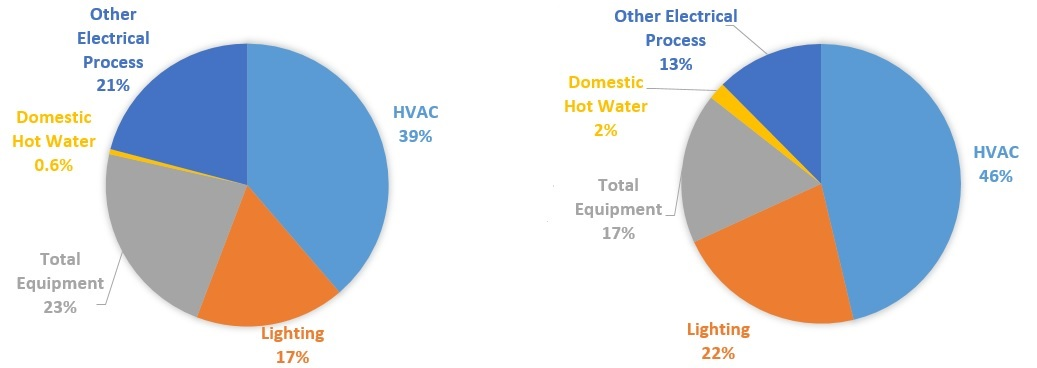
\includegraphics[width=5in,keepaspectratio]{figs/intro_end_use_split.jpg}
%\end{tabular}
\caption{Electricity consumptions of commercial offices and universities by end use in the United States (left) \& Australia (right).}
\label{intro:electricity_end_use_split}
\end{figure}
\noindent two countries, they epitomize the end-use split of electricity consumption in most commercial offices and universities worldwide.

With rising energy costs and increasingly stringent regulatory environments, improving the energy efficiency of HVAC operations in buildings has become an important issue. From a short-term economic point-of-view, with over 100 billion dollars in annual electricity expenditures even a small percentage improvement in the operation of HVAC systems can lead to significant savings. From a long-term point-of-view, the need of fostering a smart and sustainable built environment calls for the development of innovative HVAC control strategies in these buildings. 

%--------------------------------------------------------------------------------------

\section{Problem Addressed}
\label{sec:problemstatement}
%I believe A is better than B.
 
There are substantial opportunities to reduce the HVAC energy consumption in commercial offices and universities, given their significant energy consumption. %through optimisation. 
%Occupants’ HVAC usage is largely dependent on their activities.
%Appropriate scheduling of the occupants’ activities in commercial/educational buildings helps to proactively control HVAC operations.

In conventional building operations, HVAC systems run according to a pre-defined occupancy schedule. They maintain a minimum air flow rate to ensure prescribed indoor air quality standards, and keep the zone temperature within a pre-defined comfort range using real-time temperature measurements in a {\em reactive} manner. One weakness of this control logic is that it ignores occupancy dynamics: it treats unoccupied zones of the building in the same way as occupied ones, which results in substantial energy waste.

Recent studies have shown that energy consumption can be significantly improved by adopting more complex control strategies that exploit measured or predicted occupancy information \citep{agarwal2010occupancy, erickson2010occupancy, erickson2009energy, goyal2013energy, goyal2013occupancy, west2014trial}. For instance, model {\em predictive} control strategies determine supply air flow rate and temperature over longer time horizons in such a way as to optimise energy consumption, whilst remaining within air flow and temperature bounds that reflect the predicted occupancy of various building zones \citep{goyal2013occupancy}. These strategies are naturally capable of pre-cooling zones if this reduces consumption or if it is necessary to meet the comfort bounds. %However, these approaches do not perform occupancy scheduling, and ignore the fact that some schedules may lead to more energy savings. 

Another body of recent research has investigated the {\em proactive} control of {\em occupancy} in order to minimise HVAC consumption \citep{chai2014minimizing,klein2012coordinating,kwak2013tesla,majumdar2012energy,pan2012thermal}. Many office and university buildings offer some scope for occupancy control via their room booking and scheduling systems. For instance meetings, lectures, exams, use of special purpose rooms, and other short-term activities can be scheduled to occur at times and in rooms that are beneficial from an energy standpoint.
Unfortunately, existing occupancy scheduling approaches assume conventional HVAC control strategies \citep{kwak2013tesla}. Moreover, since working from first principles using models of the HVAC and the building is computationally expensive, they typically adopt suboptimal scheduling strategies guided by proxies for the optimisation criterion. One such proxy is the minimisation of the number of rooms used and of the time gap between successive meetings; it is used to guide the search towards solutions that take advantage of thermal inertia and schedule meetings to take place back-to-back in as few rooms as possible \citep{pan2012thermal,majumdar2012energy}.

In this thesis, we go an important step beyond existing work: we look at the potential for integrating building operations with room booking and occupancy scheduling, and combine the benefits of both research trends above. 
%Specifically, energy consumption in commercial offices and educational buildings is impacted by group activities such as meetings, workshops, classes and exams, and can be reduced by scheduling these activities to take place at times and locations that are favorable from an energy standpoint. 
More specifically, we explore a new way of reducing HVAC consumption in commercial buildings, by jointly optimising the occupancy scheduling decisions and the building's occupancy-based HVAC control. %, by allowing the occupancy scheduling decisions to rely on an explicit model of the building's occupancy-based HVAC control. 

As mentioned before, existing work considers either one or the other subproblem: either scheduling occupancy given conventional control policies, or HVAC control using a given occupancy schedule. 
From a computational standpoint, the joint problem is much more challenging than either, as HVAC models are traditionally non-linear and non-convex, and scheduling models additionally introduce discrete variables capturing the time slot and location at which each meeting is scheduled. This problem is regarded as a non-linear hybrid discrete-continuous problem, which is challenging to solve and optimise. A core aspect of this research will thus be to design models that are amenable to optimisation, while being sufficiently accurate. 

The key research question we tackle in this context poses a substantial challenge but can be expressed concisely:
\begin{quotation}
		\emph{Can we design optimisation methods that integrate occupancy scheduling with HVAC control, in such a way that the HVAC consumption is reduced, while the occupancy thermal comfort and scheduling requirements are addressed?}
\end{quotation}

In answering this question, we will provide a holistic approach that improves the energy efficiency of HVAC operations in buildings over state-of-the-art mechanisms. This will allow the HVAC systems to operate more efficiently and at lower cost. Building occupants will benefit through effective controls that assure their thermal comfort, while reducing their carbon footprint.

We identify four unique research challenges that should be simultaneously addressed in order to achieve our goal, which form the motivations for the work in this thesis:
\begin{enumerate}
  \item The integrated model should be computationally \emph{efficient} and achieve optimal energy reduction by fully exploiting the capability to coordinate HVAC control and occupancy scheduling. 
	\item Given sets of occupancy schedules with different constrainedness and sets of buildings with varying thermal response, the model should be sufficiently \emph{scalable} to provide instantaneous and near-optimal solutions to control and scheduling problems of realistic size.
	\item The model should be able to handle impromptu scheduling requests and respond in an \emph{online} manner.
	\item The model should enable \emph{flexible} and \emph{robust} control and scheduling, by considering the dynamics of external weather and occupants' thermal comfort preferences. 
\end{enumerate}

When combined, these parts deliver a novel mechanism that is efficient, scalable, flexible and robust for \emph{energy-aware occupancy scheduling} in commercial buildings.


%--------------------------------------------------------------------------------------
\section{Contributions}
\label{sec:contributions}
%The main challenge is that the HVAC system is rather complex and an optimisation model should model them at the proper level of abstraction to obtain optimisation models that can be solved in reasonable time. 

\subsection{Integrating HVAC Control with Occupancy Scheduling}

The first key contribution of this thesis is an integrated model that solve a \emph{joint} HVAC control and occupancy scheduling problem \citep{lim2015hvac}. Existing approaches typically solve these subproblems in isolation. A na\"{\i}ve combination would be to schedule occupancy in a first phase using existing methods, and then control HVAC based on this occupancy schedule. In contrast, we model and solve the {\em joint} HVAC control and occupancy scheduling problem. This results in an integrated approach whose benefits exceed the na\"{\i}ve superposition of both of its parts, as the scheduling fully exploits the capabilities of the underlying occupancy-based HVAC control across available times and locations.

In more detail, the joint problem we consider is that of deciding the respective times and locations (rooms) of a set of meetings or similar
activities, as well as the HVAC supply air temperature and air flow rate for each zone and time, in such a way as to optimise the overall
HVAC consumption over a long time horizon. The schedule complies with the HVAC and building dynamics models, and with comfort and air flow
rate bounds that depend on the scheduled zone occupancy. It also satisfies typical meeting scheduling constraints, including constraints on meetings times, on meeting locations (e.g. room capacity, equipment availability), and on participant attendance conflicts. 

\begin{figure}[ht]
\centering
\begin{tabular}{c}
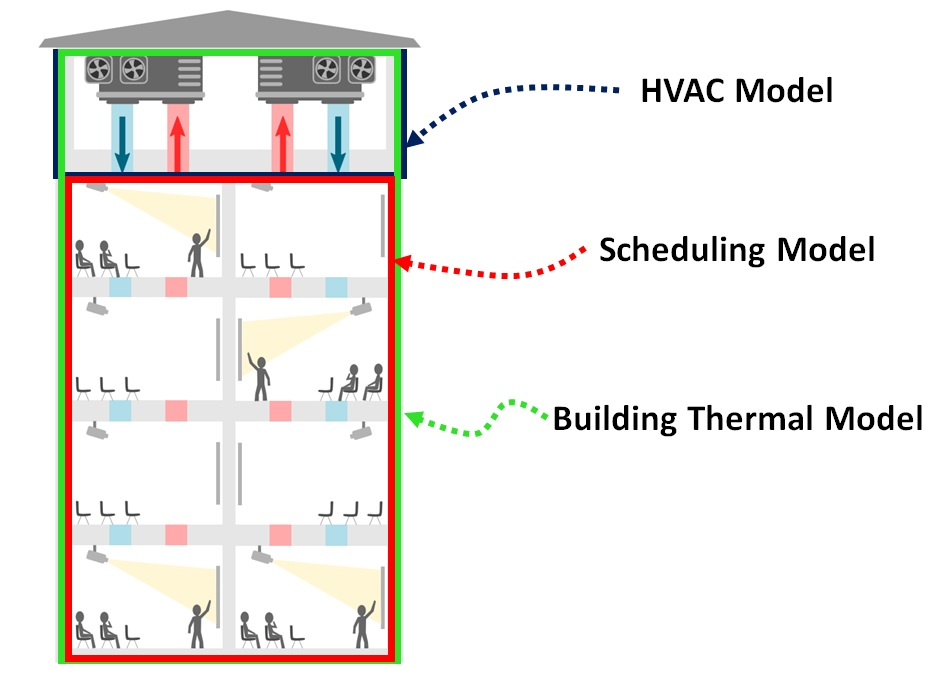
\includegraphics[width=5in,keepaspectratio]{figs/intro_three_models.jpg}
\end{tabular}
\caption{Integrated HVAC control and occupancy scheduling.}
\label{intro:three_models}
\end{figure}

Figure \ref{intro:three_models} illustrates the integration of HVAC control and occupancy scheduling in a building. To achieve this, the joint model we develop consists of three core-components: 
\begin{enumerate}
		\item A HVAC control model that simulates the physical HVAC system and allows controlling its operations, %a HVAC model that simulates the physical system of HVAC operations in buildings,
		\item a building thermal model that simulates the thermal dynamics based on internal and external heat gains, and
		\item an occupancy scheduling model that incorporates the occupancy activities, preferences and requirements.
	\end{enumerate}

Following Goyal et al. \citep{goyal2012method,goyal2013occupancy}, we focus on variable-air-volume (VAV) based HVAC systems, which serve over 30\% of the commercial building floor space in the United States \citep{eia2012cbecs}. The VAV-based HVAC systems allow us to model zone-based HVAC control, which is a crucial component for occupancy-based HVAC control. This model incorporates fan, air-conditioning and heating operations of each zone in the building, and estimates the energy consumption as a function of the HVAC control inputs (i.e. the conditioned air temperature, outdoor temperature, supply air temperature and flow rate). 

We adopt a lumped resistance-capacitance (RC)-network to model the building thermal dynamics. This model incorporates building thermal resistance, thermal capacitance, solar gain, internal heat gain and enthalpy into the estimation of zone temperature fluctuation. As buildings with different build-up (such as walls' materials, windows' facing etc.) possess different indoor climate conditions, we consider buildings with different thermal resistances and thermal capacitance. This allows us to demonstrate the energy-efficiency of different building types, and showcase the importance of picking the right rooms and times for energy savings.

Our scheduling model takes a list of meeting requests consisting of meeting time windows, duration of the meeting, list of attendees, and optionally a preferred room. We consider schedules with smaller size and constrainedness in the initial stage of our work, demonstrating the benefit of our model over existing approaches. We then introduce schedules with higher complexity and constrainedness to showcase the scalability of the model.

When combined, these three core components form an integrated model that determines the times and locations of a set of occupant activities, and a set of HVAC control inputs (i.e. the supply air temperature and air flow rate) for each zone, in such a way as to minimise HVAC consumption.

Our initial model consists of a mixed-integer non-linear programming (MINLP) model. What makes this especially challenging is the presence of bilinear terms in the HVAC control, which involves non-linear non-convex constraints. To address the challenges caused by the presence of non-linear HVAC control constraints, we relax them in a principled way using McCormick's relaxation to obtain a mixed-integer linear (MILP) model guaranteed to provide a lower bound on the objective function. Given the highly-constrained nature of meeting scheduling with HVAC control, solving the integrated problem as a MILP seems to be a reasonable choice. MILP easily manages the interaction between meeting scheduling and the impact it has on HVAC energy consumption.

%We then introduce the concept of outdoor air economy cycle into our integrated model. Economy cycle is a strategy of using 100\%of ourside air to provide ``free cooling'' when conditions permit.  %The presence of discrete variables in our HVAC model facilitates the introduction of a standby mode for operating out of business hours. 
As a further refinement, we then introduce a HVAC standby mode for operating out of business hours in our integrated model. In conventional operations, the HVAC is turned off outside of business hours (typically 6pm-6am) and restarts early in the morning to ensure that building temperature is comfortable by start of business. With our standby mode, the HVAC can decide to re-activate at night if this results in reduced consumption. Perhaps surprisingly, we show that in certain circumstances, anticipating an early morning meeting by activating the HVAC at night to cool the supply air whilst the outside temperature is still low, can reduce consumption over waiting for the pre-defined HVAC turn on time. This feature also greatly improves the \textsl{feasibility} of the solution by activating the HVAC over night to achieve targeted occupied room temperature on the next day.
%To ensure the existence of a feasible control (for adequately sized HVACs) and improve on current occupancy-based HVAC control   practices, we introduce a standby mode enabling the HVAC to re-activate at night if this is necessary to meet the temperature bounds of an early morning meeting or results in reduced consumption. 

Our results show that the integrated model achieves substantial reduction in energy consumption compared to the state of the art approaches using heuristic scheduling solutions and to more na\"{\i}ve integrations of meeting scheduling and occupancy-based HVAC
control. The MILP model developed is efficient enough for occupancy-based HVAC control, and can be used in a range of applications. Once built, such a schedule can be used in any building equipped with an occupancy-based HVAC controller by simply complementing the occupancy forecast \citep{mamidi2012adaptive} with the occupancy information captured in the schedule. Our approach can even be used with a conventional HVAC control system by constraining the bounds on supply air flow rate/temperature and the temperature setpoints to be those found in the optimal solution to the joint problem. 

\subsection{Scaling to Large Problems}

% say meetings arrival etc.
% say results show destroy room based in superior
%Large neighourhood search (LNS) model, which is approximate, and yet, precise enough to identify better quality solution within short time limit.
% Furthermore, we claim that our mechanism is \textsl{scalable} to solve control and scheduling problems with different size of complexity and constrainedness. Consequently, we will design and develop models that are capable of solving large-scale problems.

Statistics show that meeting frequency in commercial buildings is significant and continues to grow \citep{romano2001meeting,kim2014learning}. In the United States alone, fortune 500 companies are estimated to hold 11 million formal meetings daily and 3 billion meetings annually \citep{romano2001meeting}. Amongst that, 83\% of the meetings last up to 2 hours \citep{kim2014learning}. From another survey collected from the University of Southern California \citep{kwak2013tesla}, there are daily 300 unique meetings per regular day across 35 group study rooms in their university's library.

This motivates our next step where we expand our integrated model to solve large-scale problems. Our second contribution in this thesis is a Large Neighbourhood Search (LNS) approach that is capable of handling hundreds of incoming meeting requests across a large number of offices/rooms \citep{lim2015large}. The scale of control and scheduling problems grow exponentially with the number of meetings and locations. The exact method using MILP is typically too expensive for such large scale instances. Hence, to tame the problem complexity further and scale to large problems, we combine the MILP model with LNS. 

LNS is a technique for finding good or near-optimal solutions via iterative optimisation through multiple destroy and repair steps in smaller neighbourhoods. LNS is used in the destroy step to remove all meetings in a small number of randomly selected zones. MILP is used in the repair step to solve the resulting subproblem and repair the schedule to near-optimality within a limited runtime. %to form a subproblem that is capable of repairing schedule to near-optimal within a limited runtime. 
This hybrid model allows us to easily navigate through the solution space and escape local minima.

One crucial criteria of this approach is the need of identifying optimal LNS parameters that govern the behavior of the LNS heuristics. There are two key parameters to tune: (a) the number of rooms to destroy, and (b) the MIP runtime limit for the repair step. One important decision when implementing the destroy step is determining the amount of destruction. If too little is destroyed the effect of a large neighbourhood is lost and if too much is destroyed then the approach turns into repeated re-optimisation. Another important decision is whether the repair step should be optimal or not. An optimal repair will be slower than a heuristic, but may potentially lead to high quality solutions in a few iterations. 

There are numerous values that these parameters can take on. As a result, some parameter tuning will be essential in achieving good performance overall. We use the sequential model-based algorithm configuration (SMAC) methodology \citep{hutter2011sequential} on an independent set of problems to optimise the parameters of the number of rooms to destroy and the MILP run time. Specifically, we generate problem instances with different degrees of constrainedness and train the parameters to achieve the best quality for all input scenarios.

What we find in our experiments is that this approach is reasonably responsive and fast in providing near-optimal solutions. Given benchmark sets of different complexity and constrainedness, the model outperforms the MILP model in terms of (a) solution optimality given a time limit, and (b) solution feasibility of the HVAC control and occupancy scheduling.


\subsection{Handling Online Requests}
%to cope with online meeting requests while regulating optimal HVAC control. 

Our third contribution is an \emph{online} approach that models and solves the joint HVAC control and occupancy scheduling problem \citep{lim2016online}. The previous two approaches are offline methods: they assume that all activities to schedule and other parameters such as the weather forecast and the solar gain are known in advance. Although both settings generate energy-efficient schedules, they nevertheless limit the practicability of the models in the real world. A recent survey shows that 56\% of meeting requests were made within 1 day before the actual meeting day \citep{kwak2013tesla}. Thus, the ability to handle impromptu requests is crucial. Moreover, the ability to update HVAC controls following a change in forecast is also essential.

Our online algorithm greedily optimises and commits to the times and locations for the latest requests, leaving the rest of the current meeting schedule fixed but revising the entire future HVAC control strategy. This ensures that whilst participants are instantly notified of the scheduled time and location for their requested activity, the HVAC control is constantly re-optimised and adjusted to the full schedule and weather updates. 

As in the offline case, we formulate the online model using mixed-integer programming (MIP), and combine MIP with large neighbourhood search (LNS) so as to scale to problem with large number of online requests and building zones. Given the relatively smaller number of meetings in online scheduling compared to offline scheduling (while the search space remains large in terms of the number of building zones), this hybrid model is highly efficient in finding near-optimal solutions. Our experiments demonstrate that the quality of the online solution is, on average, within 1\% of that of the solution returned by the clairvoyant offline HVAC-aware algorithm \citep{lim2015large}.

\subsection{Enabling Adaptive Temperature Control}

The final contribution of this thesis explores adaptive temperature control in our joint HVAC control and scheduling model \citep{lim2016online}. Existing approaches typically assume fixed comfort bounds on the occupied zone temperature. In the fixed comfort bounds model, when a zone is occupied, the zone temperature must lie within standard cooling and heating setpoints (e.g. 21$^\circ$C-23$^\circ$C). We introduce the notion of \textsl{thermal comfort flexibility} by departing from these fixed comfort bounds. Instead of keeping the room temperature within standard setpoints, the occupants are encouraged to conserve energy by accepting some temperature deviation from the default setpoints. %They are allowed to indicate their level of tolerance to temperature fluctuation.
To achieve this, we formulate adaptive temperature models that leverage occupants' thermal comfort flexibility and outdoor temperature, and use them in a principled way to decide occupants' schedules and optimise HVAC control. 

Specifically, we explore two adaptive temperature control schemes: (a) the maximum temperature deviation aware approach (MTDA), and (b) the outdoor temperature aware approach (OATA). The first scheme limits the maximum temperature deviation allowed at any time throughout the activity period, whilst the second scheme considers the outdoor temperature. We first define a deterministic model that calculates a \textsl{cumulative temperature violation} threshold based on the selected scheme. This threshold bounds the total temperature deviation throughout the activity period, enabling adaptive temperature control whilst assuring that the thermal comfort is kept within the occupants' tolerance level. 
Whilst the deterministic model is simplistic and effective, it is hard to cope with the uncertainties on the thermal flexibility of every occupant in a meeting. To cope with these uncertainties, we resort to a robust optimisation approach. In particular, we adopt the ellipsoidal uncertainty sets approach, and provide a probabilistic guarantee to the thermal comfort satisfaction level indicated by the occupants. 
Our experiments show that, when occupants are reasonably flexible, the integration of adaptive temperature control generates higher energy savings than the fixed temperature control approach.
%These configurations are carefully chosen to be realistic enough to demonstrate the advantage of adaptive temperature control, whilst assure that the thermal comfort standard defined by the ASHRAE Standard \citet{ashrae2013thermal} is observed.  

As an additional advantage, adaptive temperature control reduces the constrainedness of our online scheduling and control problem. This can make the problem solvable when fixed temperature bounds cannot be met, which often occurs for instance when a late request needs to be scheduled in the immediate future in a room whose current temperature is far away from the comfort band. In our experiments, adaptive temperature control solves a large number of instances that are unsolvable under the fixed temperature control model.

%The final contribution of this thesis explores adaptive temperature control in our joint HVAC control and scheduling model \citep{lim2016online}. According to \cite{de1998developing}, the occupants' thermal sensations are influenced by outdoor climate conditions. They proposed an adaptive comfort temperature scheme, which shifts away from fixed indoor comfort bands towards wider temperature operating bands based on outdoor temperature. Recent work \citep{egan2010the} shows that even a narrow variation of comfort temperatures can achieve significant energy savings. 

%We introduce the concept of robust optimisation into the online model in chapter \ref{cha:online}. Unlike the online approach with fixed temperature bound, in this robust formulation, the comfort constraints are relaxed in a way that allows the thermal comfort conditions to be violated for a limited amount of time. We implement both adaptive temperature control methods with three flexible comfort levels  defined: low, medium and high settings. Each setting has different input configurations that reflect the occupants' level of thermal comfort flexibility. These configurations are carefully chosen to be realistic enough to demonstrate the advantage of adaptive temperature control, whilst assure that the thermal comfort standard defined by the ASHRAE Standard \citet{ashrae2013thermal} is observed. 

%\textcolor[rgb]{1,0,0}{Need rewrite clearer!!!  Inspired by these works, we introduce the notion of thermal comfort flexibility in our model by allowing occupants to indicate their level of tolerance to temperature fluctuation. We explore two different schemes. The first scheme sets the maximum temperature deviation allowed any time, whilst the second scheme uses outdoor temperature to derive a threshold limiting the temperature violation. Both schemes are formulated into low, medium and high flexibility level, which simplify the occupant's choices for different tolerance ranges. We then solve a robust optimisation model which provides a probabilistic guarantees to the temperature violation threshold. Our experiments show that, when occupants are reasonably flexible, the integration of adaptive temperature control generates higher energy savings than the fixed temperature control approach.}


\section{Potential Integration with Building Management Systems}

We have developed a working prototype for the mathematical models discussed in Section \ref{sec:contributions}. In this section, we explore the potential of integrating this prototype with building management systems (BMS). 

%While it is possible to reduce energy consumption by retrofitting buildings with more efficient HVAC systems, it is far more cost effective to improve their control algorithms. A building management system (BMS) predominantly operates on a pre-designed schedule that incorporates a nighttime setback strategy, which relaxes the comfort constraints during the night. Bloomfield and Fisk \citep{bloomfield1977optimisation} show that such a strategy leads to significant energy savings. Building management systems, however, could be far more dynamic by adopting strategies that consider occupancy information. Occupants impact the thermal behavior of buildings. For example, a BMS may relax the comfort constraints for those rooms in the building that are not planned on being used.
%While some buildings use occupancy sensor measurements to adjust lighting and in some cases adjust both lighting and ventilation, the question we address in this paper is whether proactive planning and room management via \textsl{meeting scheduling} can have an increased impact on energy savings.

This is motivated by the fact that today's BMS tend to look at the building subsystems such as HVAC control, lighting control, blind control, plug load control in isolation, not exploiting the complementary functions of the various subsystems to minimise energy consumption. BMSs also tend to be rigid, not exploiting the wealth of information on existing and future building occupancy and the forecast energy load of the building. A significant opportunity lies in integrating room and occupancy scheduling into the BMS. Research has been conducted to develop integrated and intelligent BMS systems in smart buildings \citep{honeywell2016hvac,biq2014moving,biq2014managing,lu2012integrated,smith2011energy,klee2011seven}, however none of these systems consider integrating occupancy scheduling with building operations. Indeed, the BMS at reservation times should be capable of determining which rooms are most adequate from an energy-efficiency standpoint given the expected room occupancy, the predicted temperature profile of the building's zones and the forecast outdoor weather. 

\begin{figure}[ht]
\centering
\begin{tabular}{c}
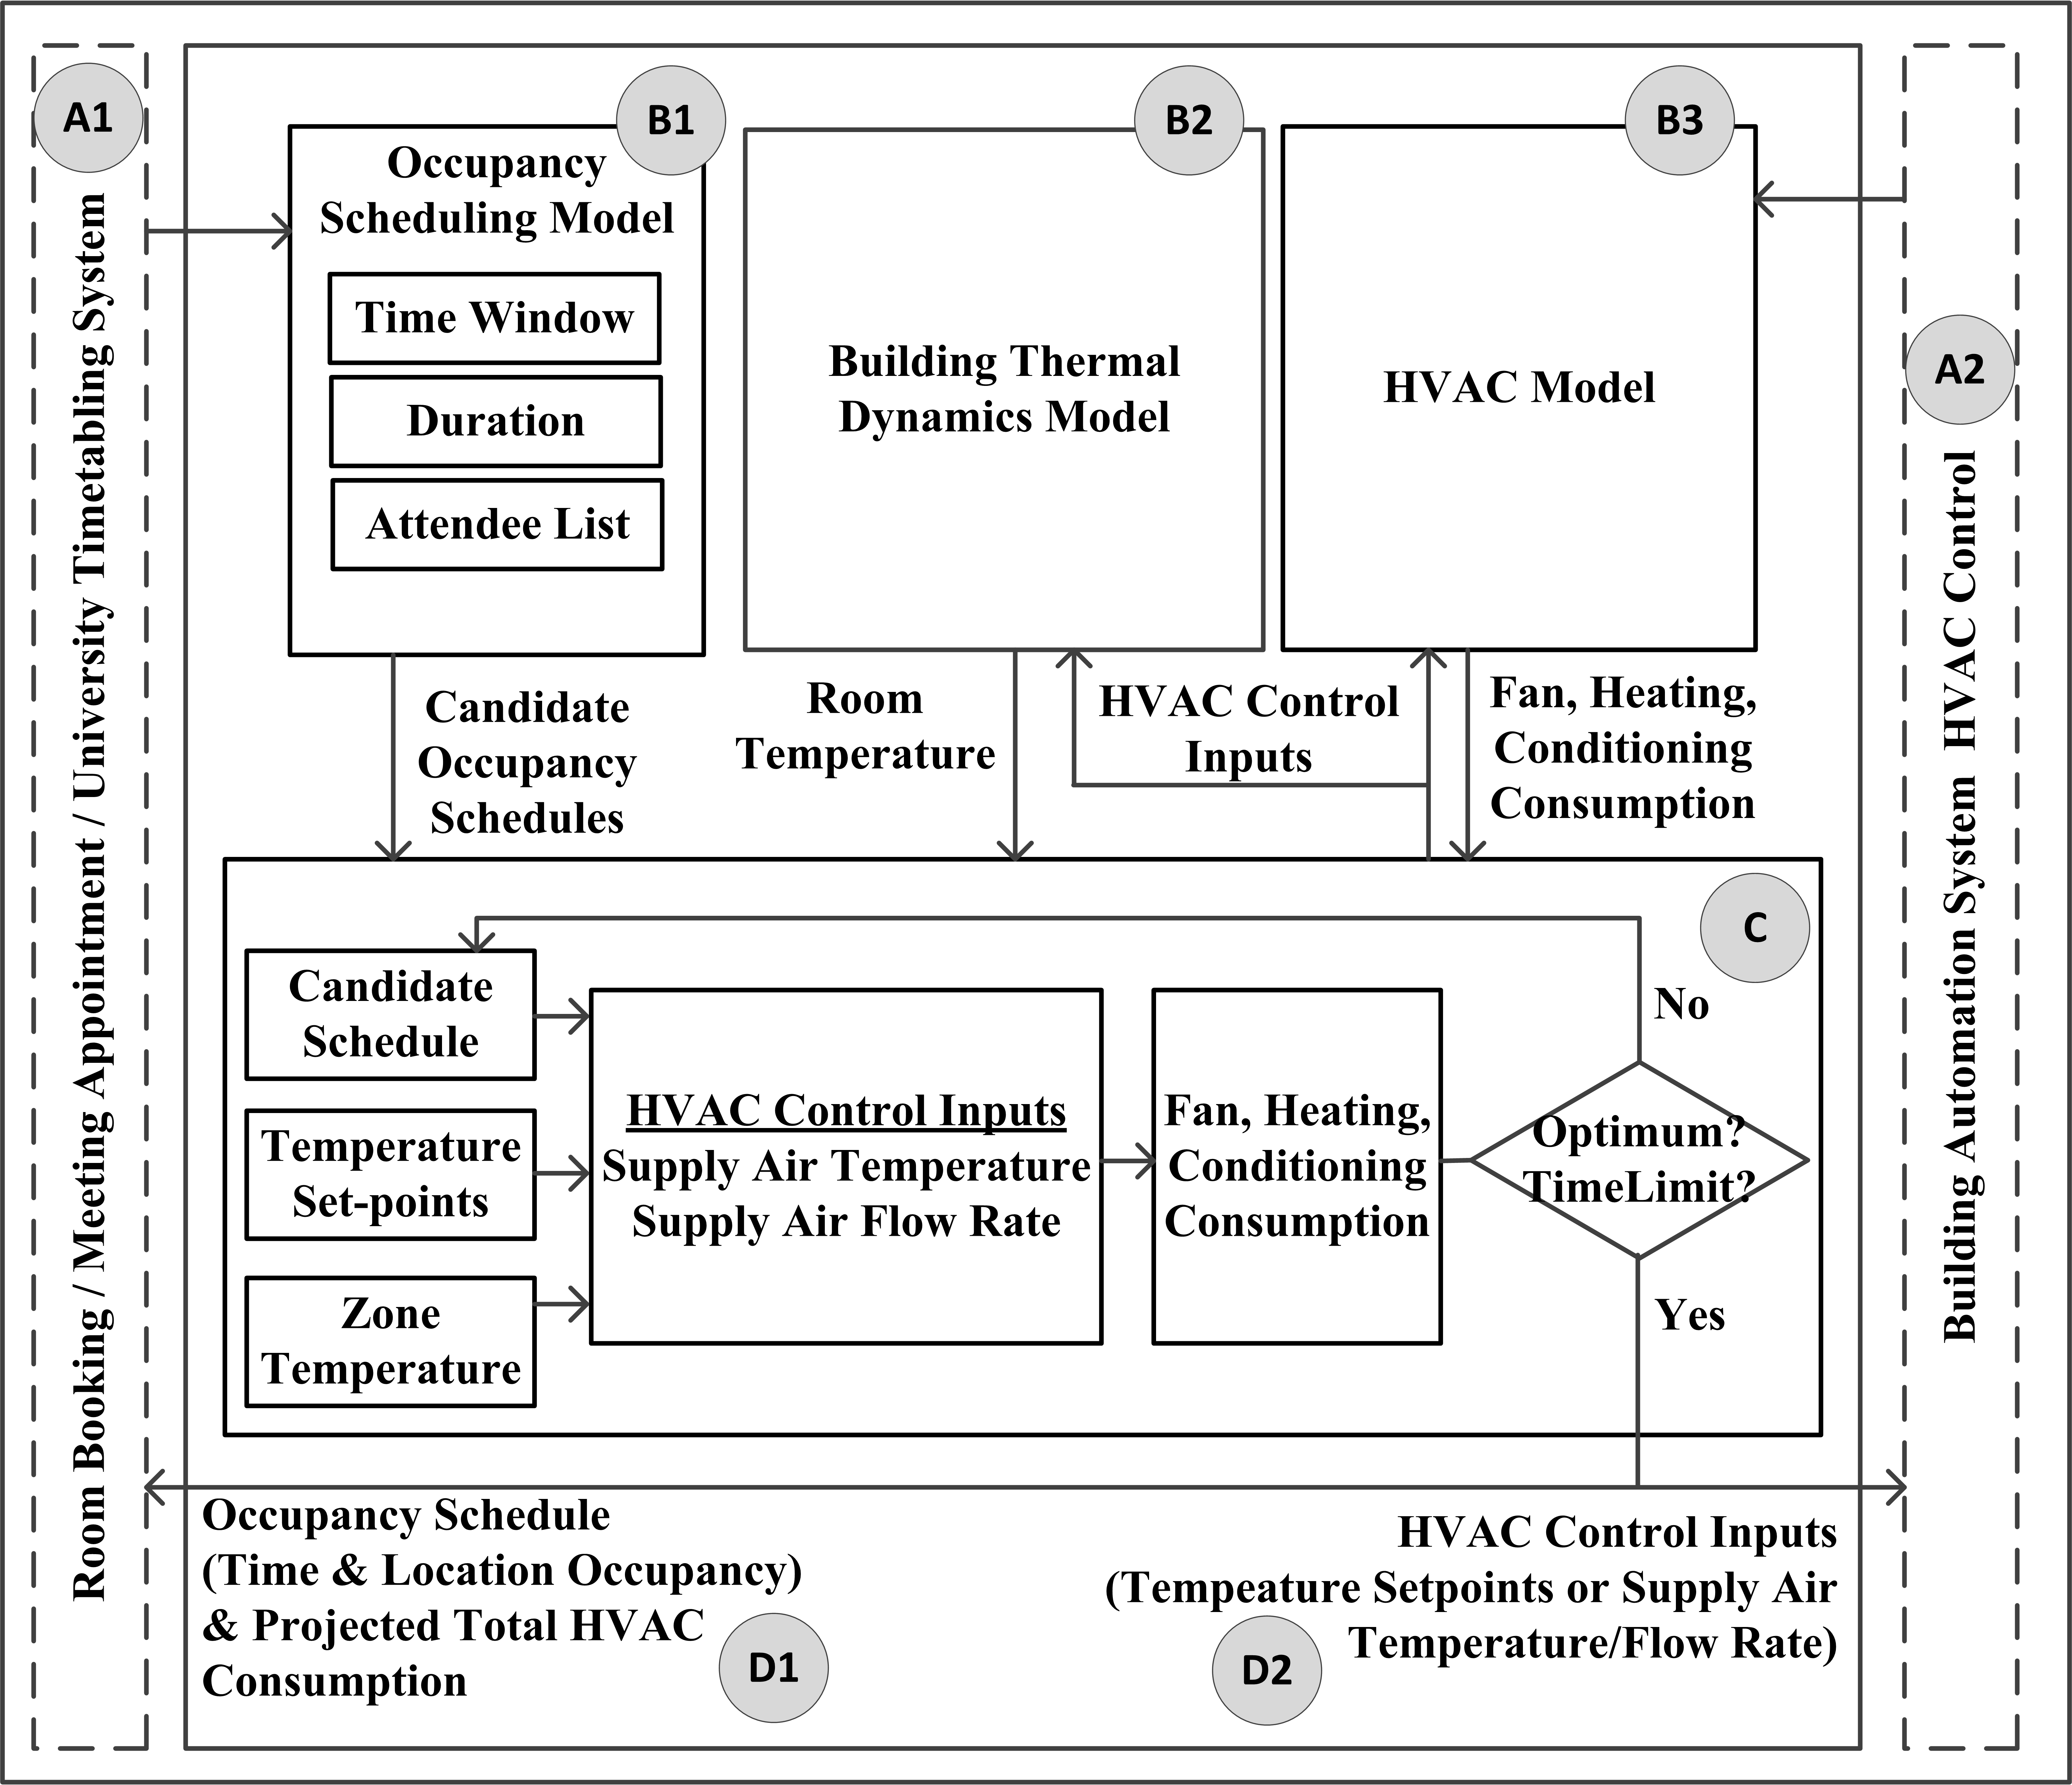
\includegraphics[width=4in,keepaspectratio]{figs/intro_eams.jpg}
\end{tabular}
\caption{Potential integration with building management system \& room booking systems}
\label{intro:eams}
\end{figure}

Figure \ref{intro:eams} illustrates how our software prototype can be integrated to the existing BMS system. This figure shows the input (label A), process (labels B \& C) and output (label D) of the integrated system. Our system receives the following as inputs:  
\begin{enumerate}
	\item a set of occupancy requests including time windows, duration, attendee list, and optionally their temperature flexibility, preferred locations and facilities required from the occupancy management system (A1). These system can be either a room booking system, a meeting appointment system or a timetabling system, and
	\item the buildings physical model, the components settings and the components limitations of the building's HVAC control from the Building Automation System (A2).
\end{enumerate}

These inputs allow us to calculate and configure appropriate constant values and constraints for the scheduling model (B1), the building thermal dynamic model (B2) and the HVAC model (B3). We then run our integrated model (C) to identify the optimal HVAC control and the best occupancy schedule that maximise energy efficiency while meeting occupant comfort needs. 

The outputs consist of
\begin{enumerate}
	\item An occupancy schedule (D1), given time and location of each request, and the projected total HVAC consumption,
	\item the HVAC control settings (D2), given the zones temperature setpoints, the zone's supply air flow rate and temperature over the scheduling horizon.
\end{enumerate}

The occupancy schedule and the projected total HVAC consumption can be delivered to the occupancy management system. This information allows building occupants to track their schedule and the overall HVAC consumption of the buildings. Currently, building occupants do not usually pay attention to \textsl{when} and \textsl{where} they use HVAC. Due to the lack of informed decision about energy savings, the selections of venue and time for an activity are often determined by their preferential choice. Now, with the energy consumption information provided, they are given an option to make an environmental friendly decision according to their schedule. 

The HVAC control scheme consists of the temperature setpoints, the supply air flow rate and temperature of each zone. This information can be selectively fed into the HVAC control system, depending on the granularity of control allowed. Currently, the temperature setpoint of each zone can be configured easily via the application programming interface of the BMS, thus this information can be used directly by constraining the comfort temperature of each zone based on our occupancy schedule. On the other hand, if the HVAC control allows a more fine-grained control, the  optimal supply air flow rate/temperature generated by our model can be used as setpoints.


\section{Summary}
\label{sec:intro_summary}

To summarise, the core research question we tackle is that how to design optimisation methods that integrate occupancy scheduling
with HVAC control, in a way that maximises energy savings whilst ensuring the comfort level necessary for occupants. We address this question in four parts that come together to form a complete solution: the formulation of a joint HVAC control and occupancy scheduling model, the development of a scalable joint model to solve large problems, the introduction of an online joint model that is capable of coping with impromptu meeting requests, and the integration of adaptive temperature control that further improves on the energy savings.

We contribute to knowledge in the area of energy-aware occupancy scheduling:
\begin{itemize}
	\item We formulate an integrated HVAC control and occupancy scheduling model using MILP, which produces efficient solutions compared to  existing approaches, and can be used in a range of applications,
	\item We develop a scalable model that combines MILP and LNS, and demonstrate that this hybrid model can effectively tackle large-scale HVAC control and meeting scheduling problems,
	\item We determine an online control and scheduling strategy based on a greedy algorithm that commits to the best schedule for the latest activity requests and notifies the occupants immediately, whilst simultaneously optimising the HVAC control parameters,
	\item We establish a robust optimisation model which enables adaptive temperature control and provides a probabilistic guarantee to the level of comfort tolerance indicated by the occupants.	
\end{itemize}

The key insight underlying this thesis is that integrating occupancy scheduling with HVAC control can lead to significant savings in energy consumption. By exploiting the synergy between HVAC control and occupancy scheduling, this approach achieves a much higher rate of energy savings than works that are based on (data-driven) black-box models of the HVAC control \citep{kwak2013tesla,chai2014minimizing} or that minimise energy consumption proxies (e.g. number of rooms used) \citep{majumdar2012energy,pan2012thermal}. Our work sets a baseline for the integration of HVAC control and occupancy scheduling in the space of energy aware scheduling in smart buildings.


\section{Thesis Outline}
\label{sec:outline}
%How many chapters you have? You may have Chapter~\ref{cha:background},
%Chapter~\ref{cha:design}, Chapter~\ref{cha:methodology},
%Chapter~\ref{cha:result}, and Chapter~\ref{cha:conc}.

This thesis is structured as follows:

Chapter 2 provides a non-technical introduction to occupancy-based HVAC control. It dedicates sections to discussing all related background: the concept of zone-based HVAC systems, building thermal model, occupancy-based control strategies, occupancy modeling and adaptive temperature control.
% the HVAC system and the building thermal model that we adopt. It also dedicates sections to discussing occupancy-based HVAC control and adaptive temperature control strategies that have been used in the HVAC domain.

Chapter 3 provides necessary background for the optimisation techniques that have been used to formulate our model. These include mixed integer programming (MIP), large neighbourhood search (LNS), online optimisation, and robust optimisation.

Chapter 4 introduces the joint HVAC control and occupancy scheduling problem, and develops an integrated model using MIP. We compare this model with the state-of-the-art occupancy-based HVAC control and heuristic-based occupancy aware scheduling, and show the corresponding experimental results.

Chapter 5 describes the LNS formulation, which integrates the MIP model with the LNS heuristics. We also discuss the automatic parameter tuning and our key observations.

Chapter 6 extends the integrated model to support online scheduling and control, and compares its effectiveness with the clairvoyant offline model.

Chapter 7 investigates the potential of adopting adaptive temperature control. We formalise the adaptive temperature control model based on robust optimisation method, experiment with different flexible setpoints control settings and demonstrate a further reduction of energy consumption compared to existing fixed temperature model.

Chapter 8 concludes our findings and combined approach, and discusses possibilities for future research.

\chapter{Background - Occupancy-based HVAC Control}
\label{cha:background}

% 1 - Talk the overall picture of occupancy-based HVAC control based on the 5 top things of first figure. Add section to first figure
% 2 - Why the reviewer need to read ur background, why is it important for your thesis... tell them how does the section links to your thesis.. ppl need to understand ur plot. "`This is important because we use it in chapter"' ... 'In chapter 1 we are considering the VAV"', "`In our thesis we adopt this RC thermal model."'
% 3 - Overall too much word, not enough equation... Add equation for R/C 

% --- add alex roger paper in RC

% Todo - 
% 	Link each section to chapters ....
% 	Revise revise revise

% xxxxxxxxxxxxxxxxxxxxxx

% HVAC control - VAV-based system
	% occupancy-based HVAC control
		% conventional control
		% model predictive control
	% adaptive thermal control
	%Link to occupancy-based hvac control, demand control ventilation, basically we focus on demand side building load instead of supply side load.
	% Building thermal dynamics - Wall R/C, occupant heat gain, solar heat gain

% Energy-aware scheduling
	% Meeting scheduling

% xxxxxxxxxxxxxxxxxxxxxx


This chapter provides a comprehensive review on occupancy-based HVAC control, which is the state-of-the-art HVAC control mechanism that optimises energy savings based on occupancy presence in buildings. This control mechanism essentially sets the context and motivation for our problem. Figure \ref{fig:background:config} provides a detailed breakdown of different aspects in occupancy-based HVAC control. These include zone-based HVAC system, occupancy-based control strategy, building thermal network modeling, occupancy modeling and thermal comfort control.

In the following sections, we describe in turn the \emph{zone-based HVAC system} that allows zone-based control, including the HVAC zoning concept, the Variable Air Volume (VAV)-based HVAC system and its operations. Next, we introduce different types of \emph{occupancy-based control strategies}, from traditional strategies, such as On/Off control, proportional–integral–derivative (PID) control, rules-based control that provide coarse-grained control based on static occupancy schedules, to advanced control strategies, such as model predictive  

\begin{figure}[hb]
\centering

\includegraphics[height=2.5in,keepaspectratio]{figs/background_configurations.jpg}	
\caption{Occupancy-based HVAC control}
\label{fig:background:config}
\end{figure}

\noindent control that perform finer-grained control based on the prediction and control of occupancy dynamics in future horizon. We then discuss various \emph{building thermal network modeling techniques} that are used to model building thermal dynamics. These techniques are important to calculate temperature dynamics in each zone and provide as an input to the feedback control system. Following that, we devote a section on \emph{occupancy modeling} and discuss how occupancy dynamics are being gathered, modeled and even proactively controlled to benefit the occupancy HVAC control system. These include using fixed schedule, sensor-based occupancy detection, occupancy prediction and energy-aware occupancy scheduling. Lastly, we talk about \emph{thermal comfort} control using fixed setpoints and adaptive setpoints.


%In Section \ref{cha:bg:hvac}, we describe in turn the HVAC system that allows zone-based control, including the HVAC zoning concept, the Variable Air Volume (VAV)-based HVAC system and its operations. Next in Section \ref{cha:bg:ctrl}, we introduce different types of zone-based control strategies, from traditional strategy that provides coarse-grained control based on static occupancy schedule, to advanced control strategy that performs finer-grained control based on the prediction and control of occupancy dynamics in future horizon. Then we discuss various thermal network modeling techniques that are used to model building thermal dynamics in section \ref{cha:bg:rc}. These techniques are important to calculate temperature dynamics in each zone and provide as an input to the feedback control system. We discuss how occupancy dynamics is being gathered, modeled and even proactively controlled to benefit the occupancy HVAC control system in Section \ref{cha:bg:occ}. Lastly, we talk about thermal comfort setpoint configurations and adaptive temperature control in section \ref{cha:bg:atc}


\section{Zone-based HVAC Systems} \label{cha:bg:hvac}

A zone-based HVAC system provides heating, ventilation and air-conditioning to different parts of a building based on pre-defined building zones. Thermostats are installed at all building zones to measure and feedback zone temperature to the HVAC system. Such zoning systems enable precise control of zone temperature based on occupancy and lead to large savings on energy bills. 

There are essentially two types of zone-based HVAC systems: Constant Air Volume (CAV)-based systems and Variable Air Volume (VAV)-based systems. CAV-based systems provide a constant air flow rate to all building zones but vary the air flow temperature to meet the thermal loads of each zone. VAV-based systems, on the other hand, vary the air flow at a constant temperature (around 13$^{\circ}\mathrm{C}$) and heat up this cold air to a designated temperature based on the heat gains or losses within the thermal zone served. Due to its greater energy savings potential, the VAV-based system is commonly preferred to the CAV-based system in mid-to-large size buildings \citep{sekhar1997critical,yao2007evaluation}.

In our work we focus on VAV-based HVAC systems, which serve over 30\% of the commercial and institutional building floor space in the United States \citep{eia2012cbecs}. These buildings are generally large buildings with a lot of rooms and open spaces with different heating and cooling needs. With VAV-based systems, we demonstrate how energy savings can be achieved by scheduling occupant activities and regulating air flow rate and air flow temperature in advance, in such a way that the VAV-based system is optimised to provide thermal comfort while conserving energy. In the following, we provide an overview of the HVAC zoning system and explain how a VAV-based system operates.% effectively to provide thermal comfort while conserving energy.

\subsection{HVAC Zoning System}

In large buildings, such as commercial offices and university lecture halls, the HVAC system must meet the varying thermal comfort needs of different spaces. The HVAC zoning system is commonly deployed to satisfy these different needs. A building is divided into different areas or ''zones``. A zone can be a single room or cluster of rooms with the same heat gain and heat loss characteristics. The division into zones enables individual control of zones' temperatures. Specifically, the building zones are designed by subdividing each floor into core and perimeter thermal zones. 

\begin{figure}[t]
\centering
\includegraphics[height=3.8in,keepaspectratio]{figs/background_layout.jpg}	
\caption{Typical office floor layout}
\label{fig:background:typical_hvac_zone}
\end{figure}

Figure \ref{fig:background:typical_hvac_zone} shows a layout of office space consisting of multiple perimeter and core thermal zones. %Consider the needs of different zones in a typical office building which have different heat loss and heat gain characteristics. 
The cubicles area and offices are arranged around the outer walls (a.k.a the perimeter zones) of the building, and a number of meeting and utilities rooms are co-located at the inner part of the building (a.k.a the core zone) with no outside exposure. %an inner core of rooms that have no outside exposure. 
% Zoning of HVAC systems typicaly separates perimeter zones that are about 5m deep from those that are in the interior. 

The perimeter zones have at least one wall or window exposed to the outside temperatures. These zones experience different heating or cooling loads based on outdoor conditions. Heat is lost from the heated spaces of the building when the outside air is colder, whilst heat is transferred to the cooler spaces of the building when the outside air is warmer. On top of that, these areas gain or lose heat at a varying rate. For example, the side of a building that is exposed to the sun has more heat gain than the sides that are shaded. The sun position, wall insulation, window build-up and blind shading all effect the heat gain and heat loss of the perimeter zones. Hence, apart from ventilation, these perimeter spaces require either heating or cooling. On the other hand, interior or core zones are unaffected by outdoor conditions and experience more or less constant loads. These zones gain heat from the interior load resulting from the presence of occupants, lights, and equipment. These spaces generally require less heating load but more cooling load. 

The cooling and heating load for both core spaces and perimeter spaces depends on many factors such as occupant density, activity level of occupants (active or passive work tasks), heat produced by equipment, type and level of lighting, and external solar gains. Since different spaces have varying rates of heat gain and heat loss, it is impossible for a HVAC system that delivers a constant volume of air at the same temperature to each corner of a building to provide similar comfort conditions. Therefore, heating and cooling must be supplied at varying rates to different zones of the building. To cater for such complex scenarios, VAV-based HVAC systems capable of providing zone-based control have become a de-facto solution. 


% http://www.achrnews.com/articles/98592-variable-air-volume-systems
%The perimeter zones have at least one wall or window exposed to the outside temperatures. \textcolor[rgb]{1,0,0}{This means that these spaces have more heat loss and heat gain than the interior rooms. On cold days, heat transfers from the heated spaces of the building to the colder outside air (heat loss). On warm days, heat transfers from the warm outside air to the cooler spaces of the building (heat gain). On top of that, these areas gain or lose heat at a varying rate. For example, when the sun strikes one side of a building, that side has more heat gain than the sides that are shaded. The position of the sun, insulation of the wall, amount of window/glass, and blind shading all affect the heat gain/loss of the perimeter zones. These perimeter spaces along the outer walls require either heating or cooling as well as ventilation. On the other hand, the core zones of the building gains heat from the interior load resulting from the presence of people, lights, and equipment. Therefore, these spaces generally require less heating except for a top floor where heat is lost through the roof. The normal condition is that they gain too much heat and therefore require cooling when occupied.} % need to say ventilation?

%The cooling load for both core spaces and perimeter spaces depends on many factors such as occupant density, activity level of occupants (active or passive work tasks), heat produced by equipment, type and level of lighting, and external solar gains. Since different spaces have different rates of heat gain and heat loss, it is impossible for a HVAC system that delivers the same temperature of air at a fixed volume to every space to provide comfort conditions for all of them. Therefore, heating and cooling must be supplied at varying rates to different zones of the building. %A zone is a space or group of spaces in a building with similar requirements for heating and cooling. All rooms in a zone can be supplied with the same temperature supply air at the same flow rate. 
%To cater for such complex scenarios, VAV-based HVAC systems capable of providing zone-based control have become a de-facto solution. 

\subsection{Variable Air Volume (VAV)-based HVAC Systems}

VAV-based HVAC systems \citep{ashrae2016sys} control air from a supply duct and vary the supply air flow and air temperature to each zone based upon the temperature in the building zone. This system is frequently associated to ''zone control`` due to its capability to maintain precise temperature control based on multiple setpoints in individual zones. %A zone can be a single room or cluster of rooms with the same heat gain and heat loss characteristics. 
This system is adopted in our model and the physical model is explained in detailed in Chapter \ref{cha:milp}.
Figure \ref{fig:background:vav} shows a schematic of a VAV-based HVAC system connected to two building zones. 


\begin{figure}[ht]
\centering
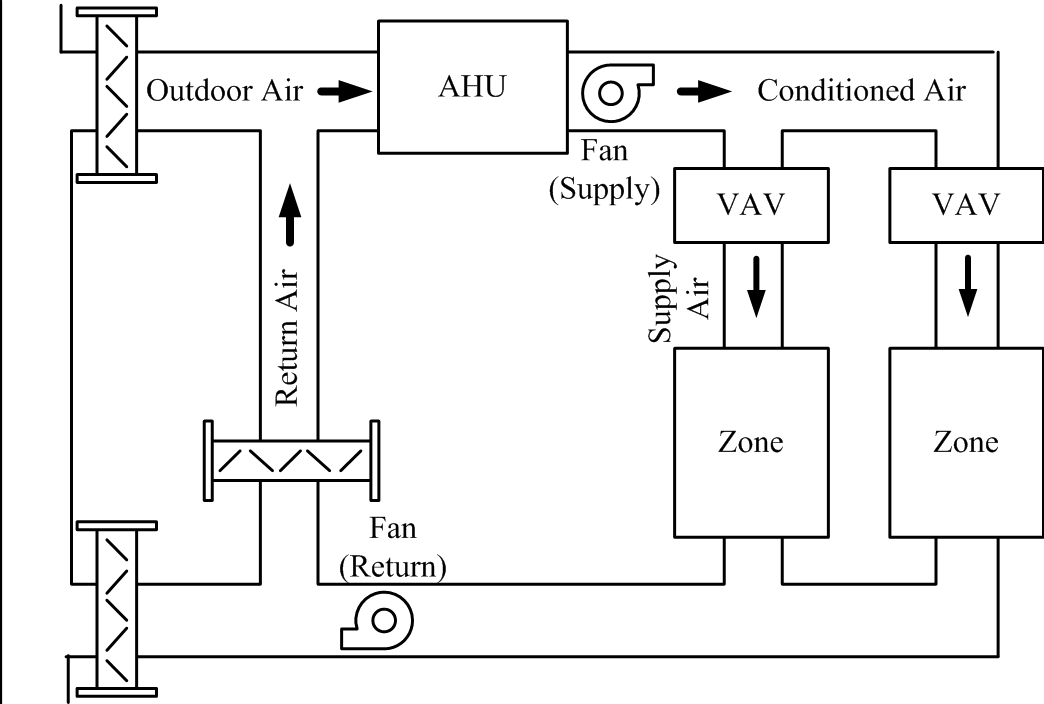
\includegraphics[height=2.3in,keepaspectratio]{figs/background_vav.png}	
\caption{VAV-based HVAC system} 
%  \textcolor[rgb]{1,0,0}{(add controller, air damper, temperature sensor, air flow sensor, actuator)}
% https://necc-controls.com/images/category/vav/johnson-controls-pneumatic_vav.jpg ,  http://www.simplyvav.com/discover/about-vav/
\label{fig:background:vav}  
\end{figure}

The main components are the central air handling unit (AHU), supply fan and VAV units. The AHU admits a mixture of outside air and return air and conditions it to a pre-set conditioned air temperature, usually $12.8^{\circ}\mathrm{C}$. The \emph{\textsl{conditioned air}}\footnote{The \emph{\textsl{conditioned air}} is sometimes referred to ''supply air`` in other literature. However, following \cite{goyal2013occupancy}, we denote as \emph{\textsl{conditioned air}} the cold air distributed by the air handling unit to the supply duct prior to reaching the VAV unit, and as \emph{\textsl{supply air}} the cold air or re-heated air that flows through VAV unit into each zones.} is then distributed through the supply air duct to a network of VAV units in the building. %Each zone has a VAV unit connected to the supply duct. 
A VAV unit is a small metal box located in the supply air duct just before the outlet of each zone. This terminal unit is also called a VAV terminal, VAV box or outlet box. 
The VAV unit is equipped with a few essential components:

\begin {enumerate} [label=\alph*\upshape)] %[label=\itshape\alph*\upshape)]
\item a temperature sensor that monitors each zone temperature,
\item an air flow sensor that monitors the volume of supply air into the zone,
\item an air damper that modulates between open and closed positions to regulate the volume of supply air into the zone,
\item an actuator that adjusts the air damper,
\item the reheat coils that heat up cold conditioned air passing through the air damper into the zone, and 
\item a VAV controller that controls and coordinates all the above operations amongst the VAV components and the AHU.
\end {enumerate} 

\begin{figure}[h]
\centering
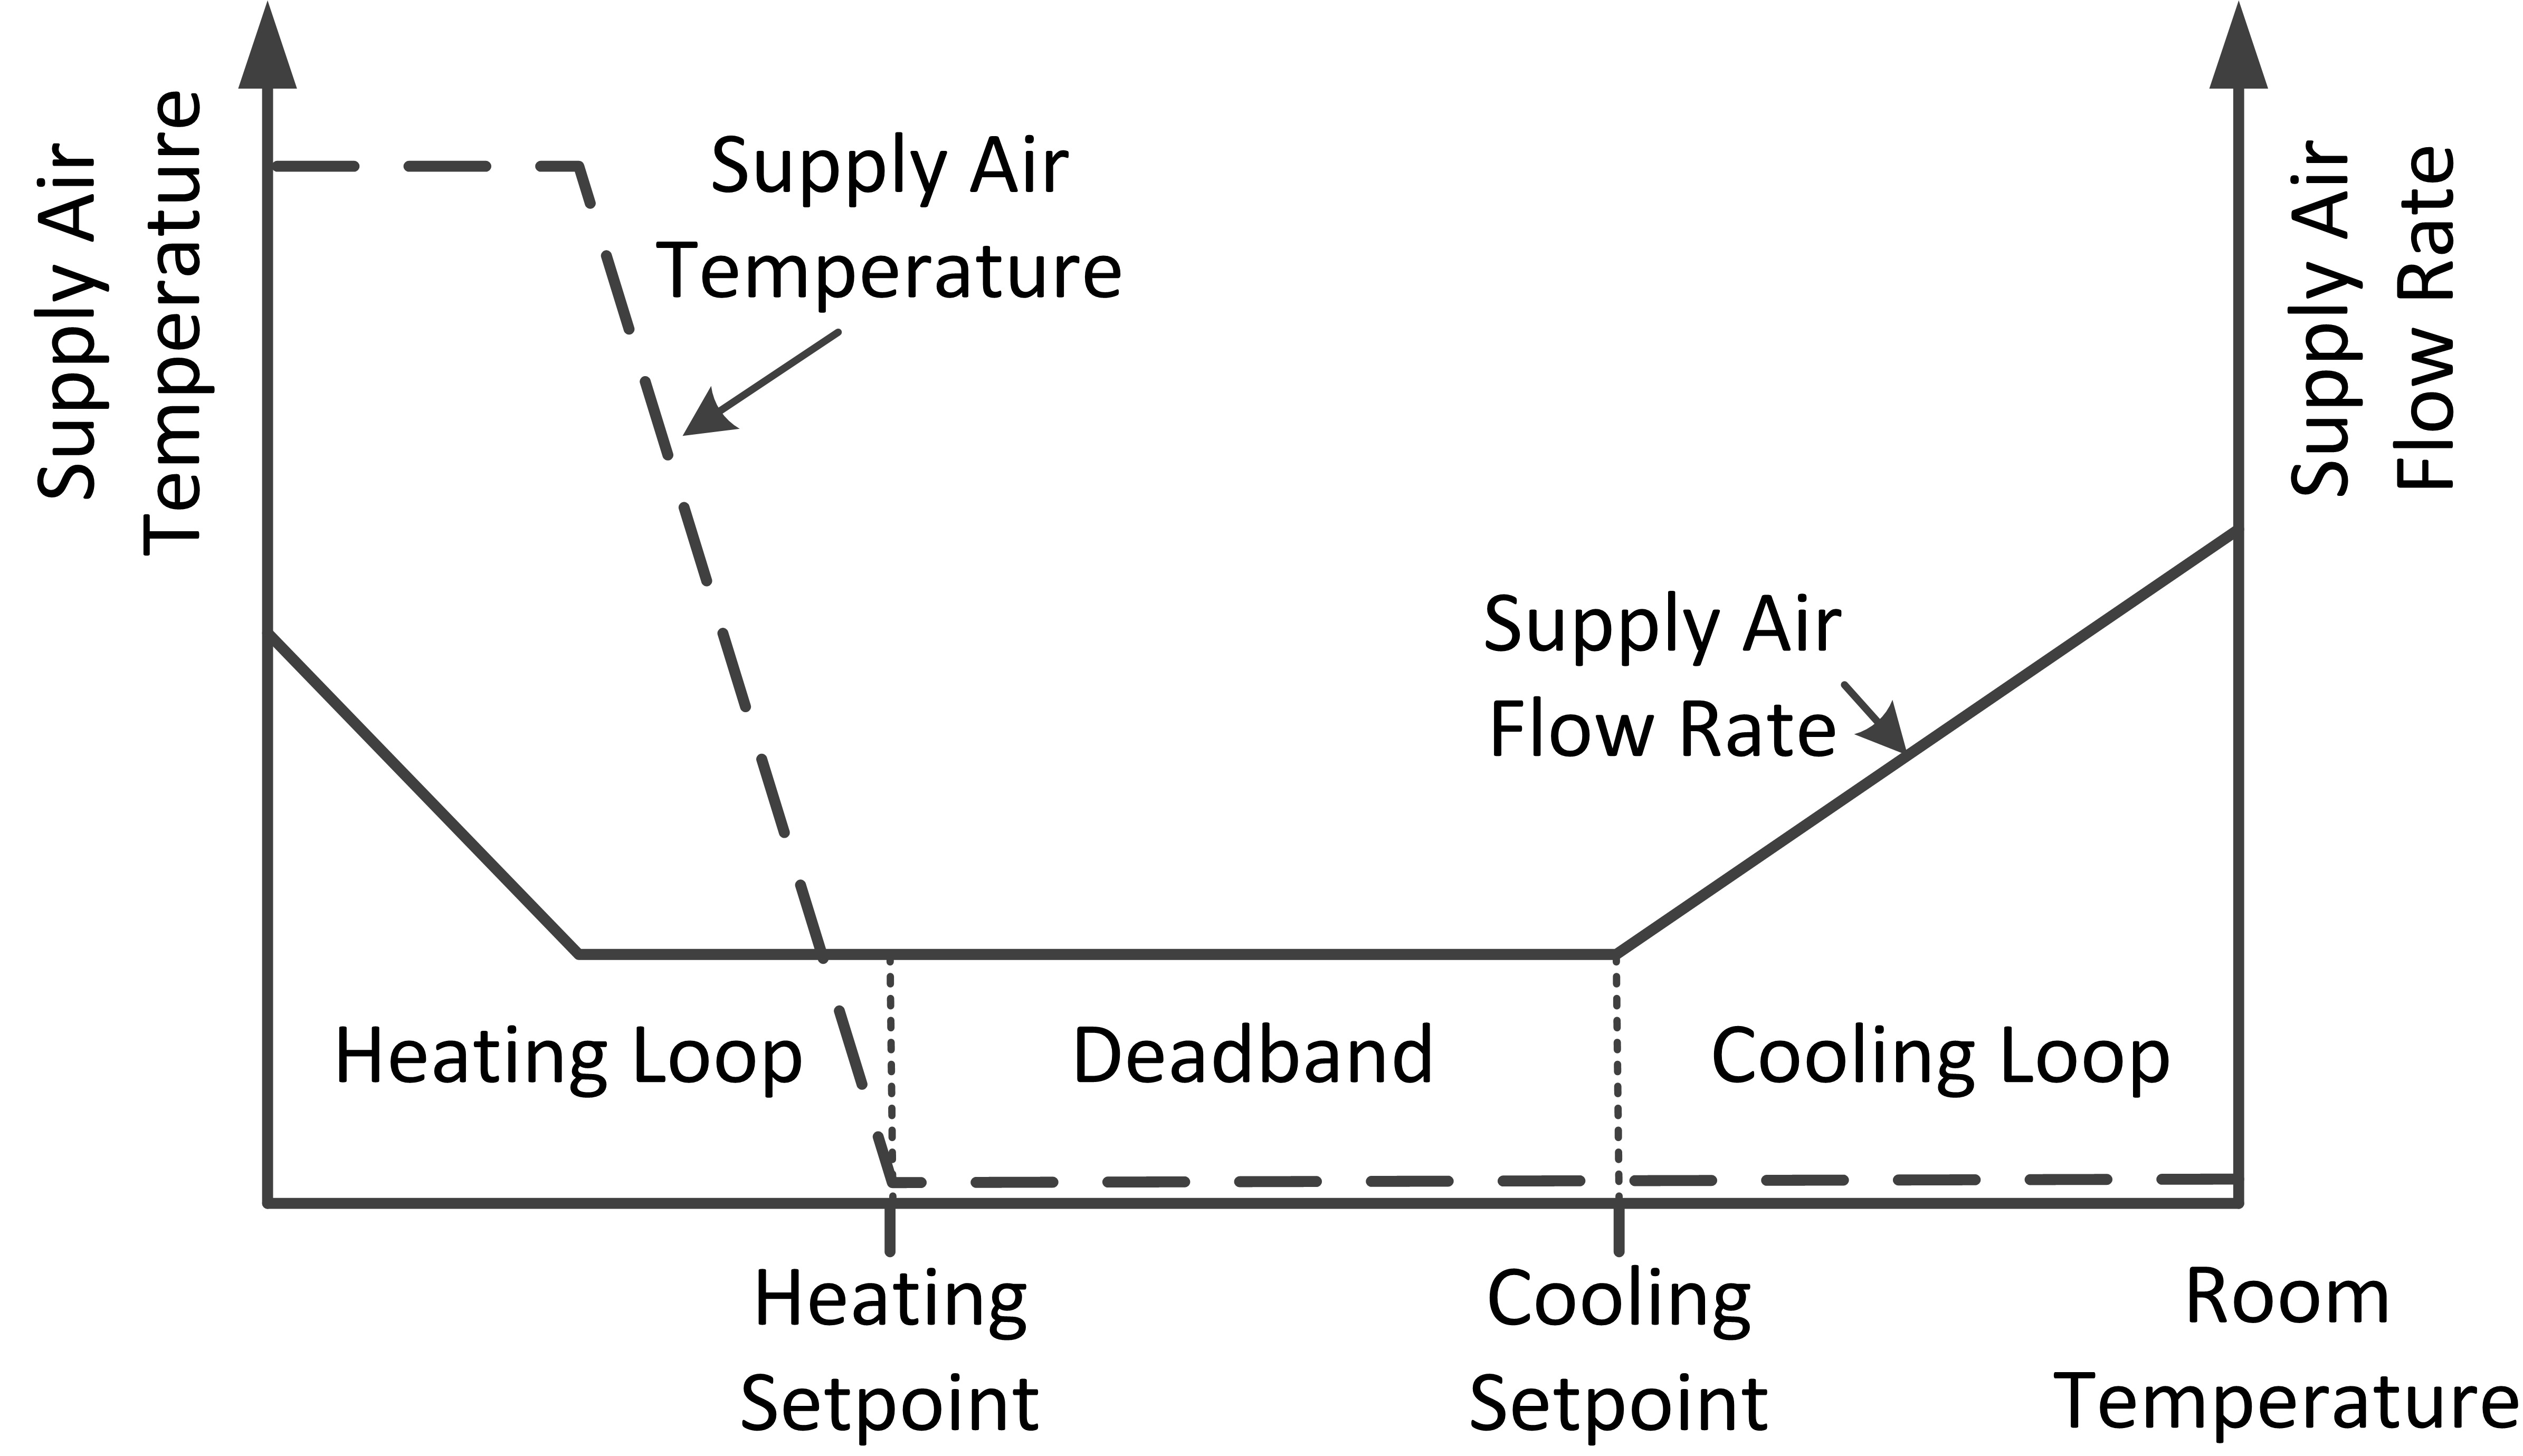
\includegraphics[height=2.5in,keepaspectratio]{figs/background_dualband.jpg}	
\caption{Dual maximum VAV setpoints control logic}
\label{fig:background:dualband}
\end{figure}

Each VAV unit receives conditioned air from the central AHU at the same temperature. As the conditioned air temperature is constant, the \emph{\textsl{supply air}} flow rate and supply air temperature into each zone must vary to meet the rising and falling heat gains or losses within the thermal zone served. Figure \ref{fig:background:dualband} shows a schematic representation of a ''dual maximum`` setpoints control logic used at the VAV units. Each zone has a pre-defined heating setpoint and a pre-defined cooling setpoint. 
In this control sequence, at peak cooling the VAV controller opens the air damper until the supply air flow reaches a pre-defined upper limit. This allows the VAV unit to discharge the maximum amount of cold air\footnote{Ideally the air temperature is similar to the temperature of the conditioned air, or the outdoor air if the temperature outside is cooler than the conditioned air.} into the zone and bring down the zone temperature. As the cooling requirement decreases, the controller modulates the air damper position to decrease the air flow into the zone. When the zone temperature falls between the cooling and heating setpoints, the system enters a deadband mode and is neither heating nor cooling. During this time, the air damper is set to open at a minimum controllable level to allow the minimum amount of air flow into the zone. In the case when a zone temperature falls below the heating setpoint, the system moves into heating mode. The control sequence is broken into two phases. In the initial phase of heating, the air flow will remain at the minimum air flow rate and the reheat coils in the VAV are turned on to add heat to the cold conditioned air up to a designated supply air temperature. If additional heating is required, the air flow rate will increase until it reaches a maximum supply air flow rate. Reheat is typically added to a few perimeter rooms or zones. Although it may seem that heating air that may have been previously cooled is wasteful, using reheat in a few locations may be more economical when both heating and cooling is required from a centralised air supply. %The reheat component is typically an electric resistance element, but hot water coils are also used for reheat.

% When the temperature sensor determines that the zone temperature is within the pre-defined comfort setpoint range, the controller closes the damper in the VAV until the supply air flow reaches a pre-defined lower limit. As the room temperature moves out of the comfort setpoint range, the controller opens the damper until the air flow reaches a pre-defined upper limit, which returns the zone temperature to the setpoint range. The exact position of the air damper varies between minimum air flow and maximum air flow as the requirements for cooling and heating in the room change. In the case when a zone requires heating, the reheat coils in the VAV are turned on to add heat to the cold conditioned air up to a designated supply air temperature. 

%In this control sequence, at peak cooling the air flow setpoint is the maximum amount of air the VAV box is set to deliver. As cooling requirements decrease, air flow decreases until it reaches its minimum setpoint. This setpoint will be based on the minimum controllable level of the VAV box or the required ventilation rate, whichever is higher. When it reaches this minimum, the system is in its deadband and is neither heating or cooling. Up to this point (cooling and deadband) the sequence looks the same as in “single maximum” logic, although the minimum air flow rate is lower. As the system moves into heating mode, the sequence is broken in the two phases. In the initial phase of heating, the air flow will remain at the minimum air flow rate and the reheat valve will modulate to full open. If additional heating is required, the air flow rate will increase until it reaches a maximum heating air flow setpoint. This maximum heating air flow is the same as the minimum air flow rate that is allowed in the “single maximum” strategy. During both of these phases, the VAV box works to maintain a constant supply air discharge temperature to the room. This requires a sensor that monitors the temperature of the supply air discharge. In the heating phases, the supply air discharge temperature should be approximately 90°F; air temperature should not be allowed to get too hot to prevent stratification and short circuiting of the hot air to the return plenum.

As each VAV unit regulates its air flow rate independently, the volume of conditioned air delivered by the central AHU varies according to the demands of the VAV units in the system. This means that the supply fan in the central AHU must vary its output in order to meet the needs of all the VAV units. If the air dampers of most VAV units are fully opened, the conditioned air required for the entire system is high. If most VAV unit dampers are closed, the conditioned air required for the system is much less. Hence the speed of supply fan is regulated to meet the changing demands of the system and to maintain a constant static pressure in the supply duct. 

%The AHU must be able to respond to the fluctuations in duct pressure caused by the individual VAV dampers constantly opening and closing. In addition, it must meet the various demands of individual VAVs. A VAV controller interacts with the AHU through 
%A particular VAV controller does not actually ''force`` the AHU to do anything. Rather it sends requests such as ''send cooler air``. Through its own controller, the AHU determines how to respond to the numerous and varied demands of the VAV units it is serving.

% Instead of just VAV, says  Today, a BAS controls and coordinates VAV, AHU, chiller, boiler etc.
%   https://en.wikipedia.org/wiki/Building_automation
Most VAV systems and the AHU are coordinated and controlled through a centralized building automation system (BAS). Each VAV unit can send information and receive instructions from the BAS, allowing more complex control and optimisation of the HVAC operations. Alternately, the BAS can continually poll each individual VAV controllers, looking for information such as damper position, room temperature, supply air flow rate, and supply air temperature. It can also send remote control instructions to each individual VAV units, such as controlling the damper position, supply air flow rate and supply air temperature into each zone. 

Overall, the main advantage of a VAV-based HVAC system is its capability to ensure occupant comfort and avoid energy waste. Indeed, a building with many VAV zones raises the chances of thermal comfort satisfaction with zone-specific temperature setpoints control. Having many VAV zones also reduces the chance of over-cooling or overheating which lowers fan speeds and lowers the central conditioning requirement, both of which result in lower energy use. 

However, the main issue is that configuring a truly ``high performance'' VAV system, including determining the optimal start/stop of the system, detecting zone occupancy, varying air flow of each zone, optimising fan-pressure optimisation, resetting conditioned-air temperature, optimising zone ventilation etc., is an extremely challenging problem \citep{murphy2011high}. The research and development of these zone-based optimal control strategies has been an ongoing concern in the fields of \emph{\textsl{occupancy-based control}} (OBC) and \emph{\textsl{demand-controlled ventilation}} (DCV), which we describe next %, considering that the zone-based control strategies are essentially depending on the occupancy and the ventilation demands of each zone 
\citep{xu2009model,erickson2010occupancy,liu2012review,balaji2013zonepac,oldewurtel2013importance,goyal2013energy,goyal2013occupancy,zhang2013energy}.

%In the following sections we describe various aspects of occupancy-based HVAC control. We discuss their mechanism, the pros and cons of the system. They range from .... to ....
%Several design and control strategies that can significantly reduce energy use in multiple-zone VAV systems have been proposed. However, implementation of them in buildings seems to be surprisingly infrequent.
%\textcolor[rgb]{1,0,0}{vs .CAV-system, say VAV/CAV are demand side system, there are other supply side system too...}


\section{Occupancy-based Control Strategies} \label{cha:bg:ctrl}

The need for comfort control arises because buildings are occupied.
%The primary reason for building comfort control is because it is occupied.
In practice, however, in the majority of buildings the indoor conditions are either pre-defined or reactive based on temperature sensors. A standard practice is to preset building temperature at a comfortable range, for instance between 20$^\circ$C to 24$^\circ$C during standard operating hours regardless of its occupancy. This practice incurs high energy cost and causes a waste of energy used to heat up or cool down vacant zones. 

The goal of occupancy-based HVAC control is to use occupancy information to reduce energy use -- over conventional control algorithms -- while maintaining thermal comfort and indoor air quality. This control strategy regulates the indoor climate of a building based on either pre-defined, measured or predicted occupancy information. In this section, we discuss various control strategies used to perform occupancy-based control, ranging from conventional control strategies using pre-defined occupancy schedules to advanced control strategies that predict occupancy flow over a control horizon. Conventional controls such as on/off control, PID control and rule-based control are the most commonly used control mechanisms in existing commercial buildings, whilst model predictive control (MPC) is becoming the de facto control strategy in new buildings due to its advanced features that yield higher energy savings.
%Various control mechanisms have been developed to perform occupancy-based control, ranging from basic control strategies that use conventional on/off control, PID control and rule-based control methods, to advanced control strategies that use model predictive control (MPC) approaches. % to optimise HVAC over a control horizon using occupancy information.

Based on the occupancy information, these control mechanisms are used for the dynamic control of the demand-side of the HVAC system, including VAV dampers position control, heating coil control, supply air temperature control, supply air flow rate control and room temperature control. They are also used at the supply side of the HVAC system for controlling the conditioned air temperature set point of an AHU, the chilled water temperature setpoint, the outdoor air ventilation rate and setpoint, the outdoor air damper control, the return air damper control and the supply duct pressure control. As the basic principle of these mechanisms are different, they can accept different level of occupancy details, thereby leading to different granularity of control.

%Conventional controls are the most commonly used control mechanisms in existing commercial buildings. These control mechanisms use classical controllers such as on/off controllers, PID controllers and rule-based controllers to operate HVAC systems. 
\subsection{ON/OFF Control}

The on/off controllers are the most intuitive and easiest to implement. It regulates processes using upper and lower thresholds, and ensures that the control parameters fall within the given bounds \citep{kolokotsa2001advanced,balaji2013zonepac}. Such controllers do not use occupancy measurements. However, they may use pre-defined occupancy schedules. Occupants are usually provided with two types of control flexibilities. They are allowed to change the HVAC occupancy status and the temperature setpoint. For the HVAC occupancy status, there are normally three types of occupancy modes: ``occupied'', ``standby'', ``unoccupied'' \citep{balaji2013zonepac}. By default, the HVAC is always set to ``occupied'' during standard operating hours. During the standard hours in the weekdays, as the zone status is likely to change once it is occupied again, the controller automatically sets itself to ``standby'' mode when the HVAC is off. During the weekends, when the HVAC is turned on, the zone status is changed to ``occupied'' mode for a few hours (for eg. 2 hours or 5 hours). For the rest of the days, the occupancy mode is always set to ``unoccupied''. Although the on/off controller is simple to implement, it fails to react quickly to dynamic processes with time lags, such as HVAC control. The HVAC processes controlled using an on/off controller display large swings from the temperature setpoints.

%The on/off controllers use an upper and lower threshold to regulate the process within the given bounds \citep{kolokotsa2001advanced,balaji2013zonepac}. These types of controllers are the most intuitive and easiest to implement. Such controllers do not use occupancy measurements; though it may use pre-defined occupancy schedules. There are usually two types of control provided to the occupants - changes in temperature setpoint and changes in HVAC occupancy status. For each of the zones, a common temperature setpoint is set. This setpoint is allowed to be changed within a bound from the preset setpoint. There are normally three types of occupancy modes: ``occupied'', ``standby'', ``unoccupied'' \citep{balaji2013zonepac}. The HVAC is always set to ``occupied'' during standard operating hours of the weekdays. When the HVAC is off during the operating hours, the controller automatically sets itself to ``standby'' mode as the zone status is likely to be changed again if occupants come into the zone again. During the weekends, when the HVAC zone is turned on, the zone status is changed to ``occupied'' mode for a few hours (for eg. 2 hours or 5 hours). Although the on/off controller is the most intuitive and easiest to implement, it is unable to control dynamic processes featuring time lags. Because of the high thermal inertia of many HVAC processes, a process that is controlled using an on/off controller displays large swings from the temperature setpoints.

\subsection{PID Control}

The PID controllers modulate controlled variables based on error dynamics to achieve accurate control of a HVAC process \citep{xu2009model,gruber2015energy}. They calculate an error rate based on the difference between a desired setpoint and a measured control variable, and apply a correction to the control variable based on the following proportional, integral, and derivative terms:

\begingroup
\begin{align*}
u_t = K^P e_t + K^I \int_0^t{e_{\tau}} d\tau + K^D \frac{de_t}{dt}.
\end{align*}
\endgroup

\noindent $u_t$ is the control variable at step $t$, $K^P$, $K^I$ and $K^D$ are non-negative coefficients for the proportional (P), integral (I) and derivative (D) terms. $P$ accounts for the present value of the error rate. Based on the model, the control output is directly proportional to the current error rate. $I$ accounts for the past values of the error rate. The integral of the error rate will accumulate over time and impact the control output. $D$ accounts for the future trend of the error rate based on its current rate of change. Using this formulation, the value of the control variable is being adjusted, with an objective to minimise the error rate over time. Note that some systems require only one or two terms to provide appropriate control. This can be achieved by setting the other term(s) to zero. In the absence of the respective terms, a PID controller is called a PI, PD, P or I controller.

PID controllers are effective to develop a supervisory control strategy for HVAC control, such as controlling the position of a damper, or the air temperature setpoint \citep{xu2009model}. For occupancy-based control, the occupancy of each zone and the total occupancy can be given as an input to the control model. This occupancy information can be retrieved from a pre-defined schedule, or measured using occupancy sensors. Generally, the PID controllers return promising results. The drawback of this model is that $K^P$, $K^I$ and $K^D$ require tunings. Thus, they are not resilient to disturbance and the performance of the controllers degrade when the operating conditions vary from the tuning conditions.
%\textcolor[rgb]{1,0,0}{The PID controllers use error dynamics and modulate the controlled variables to achieve accurate control of the process \citep{xu2009model,gruber2015energy}. These mechanisms are effective to develop a supervisory control strategy for HVAC control, such as optimising the conditioned air temperature set point of an AHU, the chilled water temperature setpoint and the outdoor air ventilation rate \citep{xu2009model}. Occupancy information can be pre-defined in a schedule, or measured using occupancy sensors. The occupancy of each zone and the total occupancy are given as an input to the control model. These controllers produce promising results, but tuning the controller parameters, such as the parameters of the cooling coil and fans, the building cooling load, pollutant load etc, is cumbersome. They are also not resilient to disturbance and the performance of the controllers degrade if the operating conditions vary from the tuning conditions. }

\subsection{Rule-based Control}

The rule-based controllers determine all control inputs based on a series of rules of the form ``if \textsl{condition}, then \textsl{action}'' \citep{dhummi2011robust,agarwal2011duty,goyal2012zone,goyal2013occupancy}. The rule-based controller in \cite{agarwal2011duty} uses occupancy measurements to turn off the HVAC system, while the controller in \cite{dhummi2011robust} modulates the supply air flow rate and the zone temperature setpoints in each zone based on measured occupancy. \cite{goyal2013occupancy} defines a set of rules to control zone temperature setpoints during occupied and unoccupied periods. Their controller is designed such that the temperature setpoints are allowed to fluctuate within a larger range when the measured occupancy is zero, and are tightened when the measured occupancy is more than one. Furthermore the controller calculates the minimum supply air flow rate based on the number of occupants in the zone. The decision of temperature setpoints is crucial as a wider range will reduce energy consumption in general, since the controller may be able to reduce reheating during low thermal load conditions and reduce the air flow during high thermal load conditions. Too wide a range, however, will lead to discomfort of the occupants. Therefore, for these types of controllers, the conditions and actions are usually associated with numerical parameters (e.g. threshold values) that need to be chosen. A good performance of the rule-based controllers critically depends on a good choice of rules and associated parameters. 

\subsection{Model Predictive Control}

Unlike conventional control mechanisms, MPC is an advanced method which uses a system model to predict the future states of the system and generates a control vector that minimises a certain cost function over the prediction horizon in the presence of disturbance and constraints. 
The optimisation model can be formulated in general form as follows:

\begingroup
\begin{align*}
\min \quad &f\left(x_{t\rightarrow t+N|t}, u_{t\rightarrow t+N|t}\right) \\
\mbox{subject to} \quad &x_{t+k+1|t} = g\left(x_{t+k|t}, u_{t+k|t}\right) \quad k=\left[0, 1,\ldots, N-1\right] \\
&x_{t+k|t} \in X \\
&u_{t+k|t} \in U \\
%\mbox{min} \quad &c^Tz	\\
%\mbox{subject to} \quad &Az = u	\quad \mbox{(linear constraints)} \\
%&\undersl{z} \leq z \leq \oversl{z}	\quad \mbox{(bound constraints)}\\
%\mbox{\emph{some or all }} &z_i \mbox{\emph{ must take integer values} \quad (integrality constraints)}
\end{align*}
\endgroup

\noindent where $x_{t+k|t}$ denotes $(t+k)$th predicted state of the system at step $t$. $u_{t+k|t}$ represents the exogenous input to the system, calculated at step $t$. The HVAC system's state trajectories are explored based on initial states and predicted disturbances (i.e. inputs) to the system, and a cost-minimising control strategy is identified until time $t+N$. 
%Only the results at step $t$ is introduced to the system as optimal inputs. 
Only the decision for time step $t$ is executed.
The prediction horizon is then shifted forward and the process is repeated all over again to calculate the optimal control signal.

Using MPC, constraints can be placed on the rate and range limits of the controlled variables (e.g. the upper and lower limits of the zone temperature, supply air flow rate limits, and range and speed limits for damper positioning). External and internal disturbances such as weather, occupant activities and equipment can also be modeled, and their predicted effects on the system are used during control vector computation. This effort results in a controller that regulates the process tightly within the given bounds, and is robust to both time-varying disturbances and system parameters. 

The main advantage of MPC is the fact that it allows the current time step to be optimised, while taking future time steps into account. This is achieved by optimising a finite time-horizon, but only implementing the control variables of the current time step. In contrast to the conventional controllers that do not have this predictive ability, MPC has the ability to anticipate future events and can take control actions accordingly. 

When applied to occupancy-based HVAC control, MPC employs a discretized model of the HVAC system, the building thermal dynamics, and exogenous inputs such as outdoor weather, solar gain, zone heat load (occupancy and equipment). It solves an optimisation problem to determine the optimal HVAC control while meeting the occupants' comfort requirement \citep{sun2010integrated,oldewurtel2010energy,nghiem2011receding,ma2011distributed,mady2011stochastic,oldewurtel2012use,goyal2012effect,oldewurtel2013importance,goyal2013occupancy,parisio2013randomized,zhang2013scenario,west2014trial,brooks2015energy}. 

Specifically, in the MPC model, the occupancy information is provided as an exogenous input. This information can be obtained from a pre-defined schedule, or predicted based on occupancy models generated using methods in Section \ref{cha:bg:occ}. The number of occupants are used to project occupancy heat gain based on the occupant activity level. For example, \cite{ashrae2013thermal} states that each occupant generates about 60W-120W based on their activity level in the office. Based on this occupancy information, the MPC model optimises the HVAC control by pre-cooling or pre-heating the room temperature to a certain comfort level prior to the projected occupied hours, while otherwise the room would stay at its setback temperature.

Conventional control methods such as PID control and rule-based control are easy to implement since they are pure feedback strategies based on measured temperature and occupancy. MPC, in contrast, requires additional information of the HVAC model, the building dynamics and the predictions of exogenous inputs such as occupancy information. Despite its computational complexity and the need for a good building thermal dynamic model, however, the MPC models reduce energy use significantly compared to conventional control schemes that are currently used to operate buildings \citep{oldewurtel2010energy,mady2011stochastic,goyal2013energy,goyal2013occupancy,brooks2015energy}. These models consistently incorporate occupancy information into the control and yield an optimal control of the building for a given occupancy prediction over sufficiently long prediction horizon; independently of any parameters and threshold values that are required to be tuned for PID control or rule-based control. In spite of high degree of uncertainty in building dynamics and exogenous inputs, \cite{goyal2012effect} and \cite{zhang2013scenario} show that MPC controller performance is robust to uncertainties, making it a good candidate for building control. 
We refer readers to \citep{afram2014theory,mirakhorli2016occupancy} for comprehensive reviews of MPC-based HVAC control methods.

% Refer to \citep{cigler2013beyond} talk more details about challenge in MPC.
MPC is adopted in our model and the details are explained in Chapter \ref{cha:milp} Section \ref{sec:mip:control}. 
The challenge of MPC is that it requires an appropriate model that adequately captures the thermal dynamics of the building, which is then used for the computation of the optimal control inputs to the zone temperatures \citep{cigler2013beyond}. This model must be sufficiently precise, in order to yield valid predictions of the relevant variables (e.g. room temperatures), but at the same time, the model must be as simple as possible for the optimisation task to be computationally tractable. %and numerically stable. 
%In Section \ref{sec:mip:control}, we show how model predictive control is adopted in our joint occupancy scheduling and HVAC control model, and how the challenge is being tackled. 
In the next section, we discuss various building thermal models, specifically the lumped RC model that is used to simulate the transient thermal dynamics of a building in our work.

%\textcolor[rgb]{1,0,0}{Say we use MPC and thermal model is an important component for MPC}In the next section, we discuss various building thermal models, specifically those that are used to simulate the transient thermal dynamics of a building in our work. % that relates the control signals to the space temperature.


\section{Building Thermal Network Modeling} \label{cha:bg:rc}

The dynamics of temperature evolution in a building is one of the most complex aspects of the overall building dynamics. The complexity lies in modeling the thermal interactions amongst rooms, occupants, equipments, outdoor climate conditions and HVAC system. The thermal interactions in a multi-zone building can be thought of as an interconnected system of many subsystems. Each subsystem corresponds to a zone, and the interconnections correspond to dynamic interactions between pairs of zones. These interactions can be either 
\begin{itemize}
	\item through conduction through the walls, 
	\item through convective air exchange among rooms or,
	\item through radiation from various material interfaces (e.g. walls, equipments and occupants). 
\end{itemize}
\noindent Incorporating these interactions in a building thermal model is a challenging task since it requires modeling heat exchange through convection, conduction and radiation among all adjacent rooms. A first-principles based model constructed from energy and mass balance equations that model all these behaviors will lead to a highly complex model \citep{goyal2012method}. 

Alternately, simpler building thermal models are sought of to simulate the thermal dynamics without losing its practicability \citep{kramer2012simplified,cigler2013beyond}. A lot of efforts have been devoted to modeling simplified building thermal network model that are applicable to computationally intensive HVAC control model, such as MPC. 
%Much effort has been devoted to modeling simplified building thermal response that are applicable for computational intensive model-based HVAC control, such as MPC. 
These simplified models include response factor methods \citep{mitalas1967room}, conduction transfer functions \citep{stephenson1971calculation}, finite difference methods \citep{clarke1985energy} and lumped resistance-capacitance (RC) methods \citep{crabb1987simplified}.

\subsection{RC Model}

%\textcolor[rgb]{1,0,0}{First explain equation of R and C, refer Gouda
%Second, put black box before grey box. Say we use white box, and say we adopt black box in EP chapter}

In our work, we focus on the lumped resistance-capacitance (RC) method.
%An extensive literature exists on modeling the conductive interaction between two spaces though the wall separating them. The most popular modeling framework consists of using resistors and capacitors to model this interaction \citep{}. 
The model is built analogously to the electrical network analogy: a thermal resistance is represented by \textsl{R} (analogously to electrical resistance) and a thermal capacitance is represented by \textsl{C} (analogously to electrical capacitance). The connecting edges represent heat flow, characterised by a temperature.
This method models building thermal response by breaking up construction elements into a number of temperature-uniform elements, about which the transient heat flow through a solid surface, such as a wall or a window, can be expressed. 
Figure \ref{fig:background:walls} depicts a construction element consisting of multiple layers of different building materials. Depending on the materials used, each layer has different thickness, thermal conductivity, specific heat capacity and density. With the lumped RC method, such construction element consisting of \textsl{n} layers of materials can be combined to form $n$ ``lumped'' thermal resistances (R) and $n-1$ ``lumped'' thermal capacitance (C). Figure \ref{fig:background:rc} illustrates an example with three ``lumped'' thermal resistances ($R^z_l$, $R^{mid,z}_l$, $R^l_z$) and two ``lumped'' thermal capacitance ($C^z_l$, $C^l_z$).

\begin{figure}[h]
\centering

\includegraphics[width=2.3in,keepaspectratio]{./figs/background_walls.jpg}
\caption{Construction element layers}
\label{fig:background:walls}
\end{figure}

\begin{figure}[h]
\centering
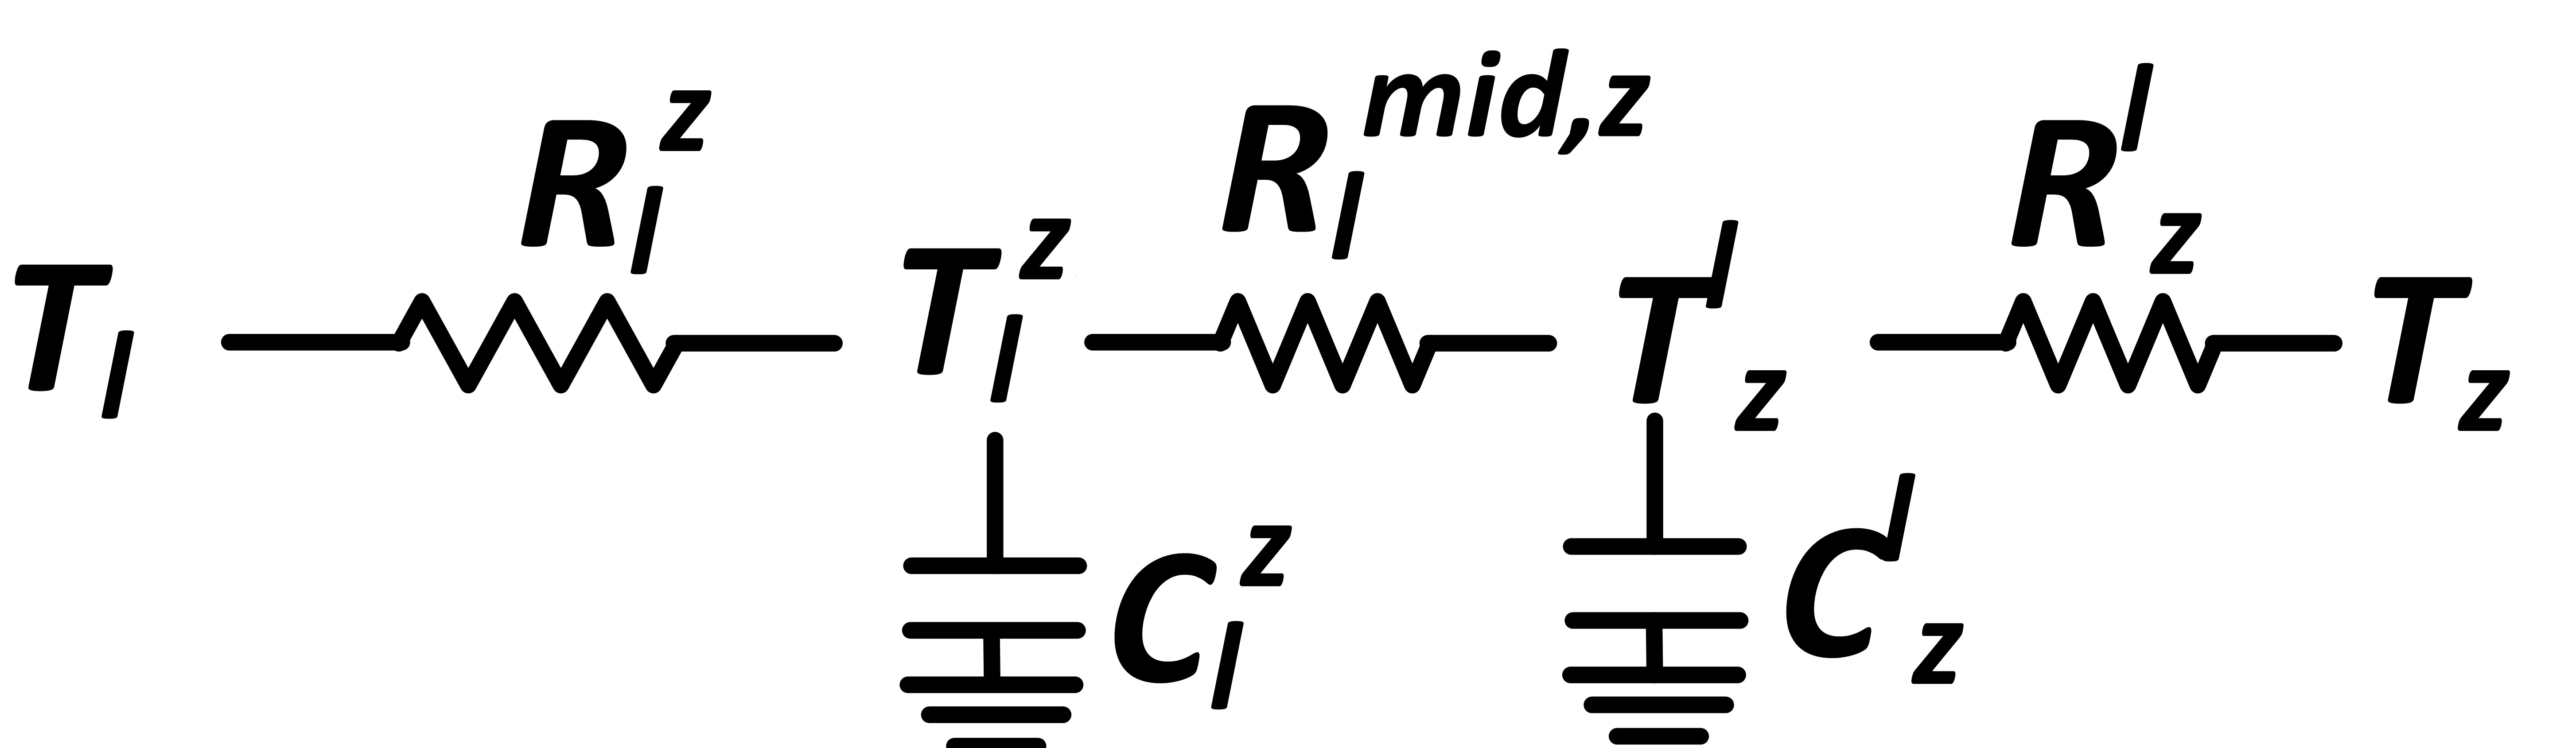
\includegraphics[width=2.3in,keepaspectratio]{./figs/background_rc.jpg}
\caption{Lumped parameter construction element}
\label{fig:background:rc}
\end{figure}

$T_l^z$ and $T_z^l$ represent the temperatures within the construction element. $T_l$ and $T_z$ represent the room temperatures at two adjacent zones. The total thermal resistance $R_{total}$ and the total thermal capacitance $C_{total}$ of each construction element can be calculated by the following equations:
\begingroup
\begin{align*}
R_{total} &= \left(\sum_{l=1}^{l=n} \frac{x_l}{k_l} \right) / A \\
C_{total} &= A \times \left( \sum_{l=1}^{l=n} x_l \times \rho_l \times c_l \right)
\end{align*}
\endgroup

\noindent where $R_{total}$ is the sum of $R^z_l$, $R^{mid,z}_l$ and $R^l_z$, and $C_{total}$ is the sum of $C^z_l$ and $C^l_z$. $A$ is the area size of a wall, $x_l$ is the length of the layer $l$ measured on a path parallel to the heat flow, $k_l$ is the thermal conductivity, $\rho_l$ is the density and $c_l$ is the specific heat capacity of the material at layer $l$.
The state equations for the thermal behaviour of each construction element can be written as follows:
\begingroup
\begin{align*}
C_l^z \dot{T}_l^z &= \frac{1}{R_l^z}\left(T_l-T_l^z\right) + \frac{1}{R_l^{mid,z}}\left(T_z^l-T_l^z\right) \\
C_z^l \dot{T}_z^l &= \frac{1}{R_l^{mid,z}}\left(T_l^z-T_z^l\right) + \frac{1}{R_z^l}\left(T_z-T_z^l\right) \\
C_l \dot{T}_l &= \frac{1}{R_l^z}\left(T_l^z-T_l\right) + Q^p_l + Q^s_l
\end{align*}
\endgroup

Note that $C_l$ denotes the thermal capacitance in room $l$, $Q^p_l$ denotes the internal heat gain from occupants and $Q^s_l$ denotes the solar heat gain.

The model order is equal to the number of capacitors used (i.e. number of \textsl{C}'s used) and for every \textsl{C}, the governing equation includes a linear differential equation. 
The resulting linear differential equation for each element can be solved analytically, making the method very computationally efficient. However, note that the model complexity increases along with the number of capacitors used. 
Thus, the capacitance and its corresponding resistances have to be carefully chosen to model the combined effect of conduction between the air masses separated by the surface, as well as radiation and convection between the surface and the air mass in contact with it \citep{goyal2012method}. 

\cite{gouda2002building} showed that a second-order lumped RC-network model with 3 resistors (\textsl{R}) and 2 capacitors (\textsl{C}) is sufficient to capture the thermal dynamic interaction between two spaces connected through a single wall. 
They showed that a reduced model based on second-order building element gives minimal loss of accuracy but significant improvements in computational effort compared to a baseline model of twenty-order lumped RC parameters benchmark. 
Thus it is possible to model the thermal interactions in a multi-zone building by using such simpler 3R2C-networks as building blocks. 

%%In this formulation, the building is represented by a network graph with nodes and edges, as in Figure \ref{fig:background:rc_network}. 
%%A node may represent a physical zone (e.g. a room, a hallway, an outdoor space) or some point inside a wall. 
%%Edges represent pathways for conductive heat flow. 
%%The air in a zone is assumed to be well-mixed so that each zone is characterised by a single temperature. 
%
%%Using these R's and C's, the network can be represented graphically as shown in Figure \ref{fig:background:zones} and Figure \ref{fig:background:rc_network}. 
%%For a zone with four adjacent walls, a window, a ceiling and a floor as depicted in Figure \ref{fig:background:zones}, the RC-network models are represented in Figure \ref{fig:background:rc_network}. 

The configurations of thermal capacitance and thermal resistances for each building elements modeled are essential. To identify the value of these parameters, three different methods can be employed:

\emph{White-box model}: This approach has a strong physical basis. The RC network's topology as well as its R and C elements (the model parameters) are derived directly from detailed geometry and construction data. For each construction element making up the building space, the layering materials, thickness, thermal conductivity, specific heat capacity and density are identified. The values of the total resistance and capacitance for each element are first calculated, and further divided into three resistance fractions and two capacitance fractions \citep{gouda2000low,gouda2002building,deng2010building,dobbs2012automatic,goyal2012method,sturzenegger2012semi,sturzenegger2014brcm}.

\emph{Black-box model}: Due to the complexity of underlying physics, a data driven approach that identifies building thermal dynamics  interactions from observed behavior is widely explored \citep{goyal2011identification,cigler2013beyond,zhou2016quantitative}. These data-driven models use techniques such as Kalman Filtering and semiparametric regression to learn the parameters of the RC network. This approach is conceptually simple but depends crucially on the availability of appropriate input data sets that encompass sufficient long sequences of all relevant feedback-response signal pairs. These are very hard to obtain from a real building during normal operation.

\emph{Grey-box model}: This first specifies a plausible RC network model using the white-box approach \citep{cigler2013beyond,ghosh2015modeling}. The model parameters are then further fitted to the building thermal dynamics using the measurements data. The advantage of this approach is that basic knowledge about possible thermal interactions can be easily introduced, and the model parameters are fitted further to a specific buildings. 


%\begin{figure}[h]
%\centering
%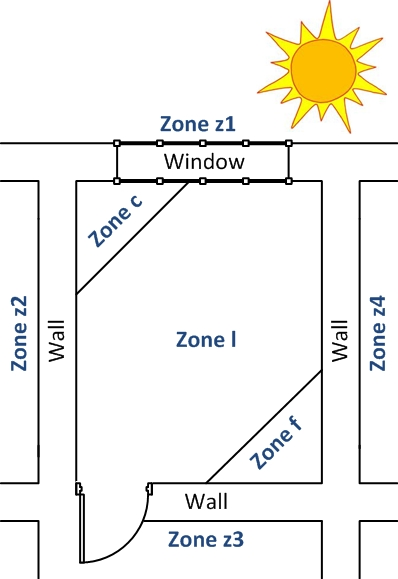
\includegraphics[width=2.3in,keepaspectratio]{./figs/zone1.jpg}
%\caption{Building with 4 zones}
%\label{fig:background:zones}
%\end{figure}
%
%\begin{figure}[h]
%\centering
%\includegraphics[height=2.3in,keepaspectratio]{./figs/background_3r2c.jpg}
%\caption{Lumped-RC network for 4 zones}
%\label{fig:background:rc_network}
%\end{figure}
%
%Figures \ref{fig:background:zones} and \ref{fig:background:rc_network} show a scenario example using lumped RC network to model the building thermal dynamics. In this formulation, a zone with four adjacent walls, a window, a ceiling and a floor ($z \in Z = {z1, z2, z3, z4, f, c}$), as depicted in Figure \ref{fig:background:zones}, is represented by a network graph with nodes and edges, as in Figure \ref{fig:background:rc_network}. A node may represent a physical zone (e.g. a room, a hallway, an outdoor space) or some point inside a wall. Edges represent pathways for conductive heat flow. The air in a zone is assumed to be well-mixed so that each zone is characterised by a single temperature.

In Chapter \ref{cha:milp} Section \ref{mip:thermal}, we adopt this lumped RC method and present a complete state-space formulation of the thermal dynamics of a building. Specifically, we use a white-box model in the settings of R's and C's. In Section \ref{cha:ep} of the Appendix, we compare our model with building energy simulation software using a grey-box model.  

The lumped RC methods have been well-explored in the recent years as they are more accurate and computationally efficient \citep{gouda2000low,gouda2002building,goyal2012method,goyal2011identification,deng2010building,ghosh2015modeling,sturzenegger2014brcm,dobbs2012automatic,ma2012demand,eisenhower2012uncertainty,radecki2012online}. Due to its practicality, this model has been widely employed by various MPC-based HVAC control mechanisms \citep{goyal2012method,goyal2011identification,ma2012demand,sturzenegger2012semi,cigler2013beyond}. We refer the readers to \citep{kramer2012simplified} for a comprehensive review of building thermal models. %the lumped RC methods as a simplified model that is near-accurate and reduces computational time is practical for MPC-based HVAC control. 

\subsection{Building Energy Software Simulation}

It is worth noting that in the HVAC community, building energy simulation software such as EnergyPlus \citep{crawley2000energyplus}, TRNSYS \citep{university2010trnsys} and DOE-2\/eQuest \citep{hirsch2010equest} are typically used for modeling building thermal behaviors. These tools contain numerous complex calculations that are useful for load calculations, equipment sizing, and predicting energy use of a building over long time intervals. However, their utility is limited as tools to model or simulate the dynamics of the thermal processes inside a building that can be used by a control system \citep{goyal2011identification}. Due to the software complexity, it is hard to seamlessly integrate optimisation algorithms with these simulation software.

Several works have also been done to compare the lumped RC model with EnergyPlus \citep{sturzenegger2012semi,dobbs2012automatic,eisenhower2012uncertainty}. \citep{sturzenegger2012semi} concludes that the understanding of wall materials and their built-up is essential to build an accurate RC model. Nonetheless, \citep{eisenhower2012uncertainty} further states that the reduced lumped RC network is robust to the uncertainty in the RC parameters of the model, and \citep{dobbs2012automatic} demonstrates that the use of model aggregation reduces computational time without significant loss of accuracy.

% Refer \citep{dobbs2012automatic} to improve on writing RC

\section{Occupancy Modeling} \label{cha:bg:occ} 

%Building occupancy varies dynamically. 
Building occupancy changes over time. 
Conference rooms, cafeterias, auditoriums, and other assembly spaces are often unoccupied for significant periods of time. Office occupancy varies during the course of a work day, from day to day, and over longer terms because of attendance of meetings elsewhere, business travel, changing room functions, and variations in staffing. The resulting over-ventilation,
during times when the space has less than maximum occupancy or is unoccupied, wastes significant HVAC energy and causes discomfort for occupants in some spaces (e.g., conference rooms) from over-cooling or overheating. In a dynamic environment where the zone settings and occupancy keeps changing, knowing occupancy information, including whether a zone is occupied or vacant, the number and identities of the occupants, is essential for occupancy-based HVAC control \citep{erickson2010occupancy,nguyen2013energy}. Thus, various mechanisms have been developed to detect, monitor, model and predict occupancy in each zone. 

\subsection{Fixed Schedule}

The most basic technique for indicating occupancy in the building involves a programmable schedule that is customizable and takes into account the occupant's activity/business hours, special events such as business trips, leaves and holidays. The HVAC system is turned on and off based on these fixed system schedules. 

\subsection{Sensor-based Occupancy Detection}

An improvement of this technique uses motion detection or Passive infrared (PIR) sensors \citep{agarwal2010occupancy} to verify whether or not occupants really are in office spaces during the scheduled times. If no motion is detected within a set time, action is taken such as changing the setpoints, or reducing minimum air flow rates into the zone \citep{zhang2013energy}. %The setback of using motion sensors is that these sensors are limited to movement and does not detect actual occupancy in a given area. 
Motion detectors provide an efficient way to detect occupancy, but they provide no information about the number of people using the space. This finer-grained information is essential to perform demand-driven temperature control and $CO_2$ ventilation. More comprehensive sensors-based and vision-based systems have been developed to achieve this goal. These systems use temperature sensors, humidity sensors, $CO_{2}$ sensors, acoustic sensors, ambient light \citep{chang2013statistical}, wireless cameras \citep{erickson2009energy}, door state sensing \citep{agarwal2010occupancy,hutchins2007modeling}, RFID \citep{li2012measuring}, communication network infrastructures \citep{melfi2011measuring,zeiler2012wireless} or combinations of various sensors \citep{yun2012building,mamidi2012adaptive,lam2009occupancy,dong2009sensor,meyn2009sensor,barakat2016agent,pedersen2017method} to provide better measures of actual occupancy. Detailed surveys of these occupancy detection systems can be found in \citep{labeodan2015occupancy,liu2012review}.

% However these sensing systems have strong dependencies on body heat accumulation and $CO_2$ concentration, which take time to build up and are a cumulative effect of various factors other than occupancy such as outdoor air quality and ventilation rate. While these systems are suitable for understanding general trends at longer time scales, they fail to respond quickly to ever changing occupancy.

%More advanced systems have been deployed, such as using cameras and vision algorithms. Extensive research has been conducted on developing occupancy detection system tat is accurate, inexpensive and easily deployable within existing buildings. 

\subsection{Occupancy Prediction}

While real time occupancy monitoring is important, occupancy prediction is also helpful for HVAC control especially with MPC. Time is required for rooms to be brought to appropriate temperatures, therefore the conditioning of the room must begin prior to when the room is actually utilised. This cannot be achieved solely by depending on real time occupancy detection. The capability of predicting occupant movement or room usage patterns is crucial to trigger HVAC control at a timely manner. %based on the estimated occupancy of a zone. 
For example if a lobby has a large number of people, then the HVAC system might predict that an adjacent conference room will be used with high probability and begin conditioning before people actually enter the room.

Various methods have been developed to understand the dynamics of occupancy patterns. The spatiotemporal dynamics of occupancy has high variability that makes this a challenging task. Determining the number of people that occupy a particular space and the corresponding duration are difficult to characterise because human behavior is considered stochastic in nature. For example, occupants do not arrive and leave at the same time of the day, their locations within the building also vary throughout the day. As a result, different zones have different hourly occupancy rates on different days. To model these occupancy behaviors and movement patterns in buildings, different approaches have been investigated and explored. These include 
\begin{itemize}
	\item statistical techniques \citep{clevenger2006impact,page2008generalised,erickson2009energy,nassar2010model,goldstein2011space,liao2011novel,duarte2013revealing,chang2013statistical}, 
	\item machine learning techniques \citep{lam2009occupancy,yu2010modeling,yang2016building} and
	\item graphical model approaches \citep{hutchins2007modeling,dong2009sensor,meyn2009sensor,erickson2010occupancy,liao2010integrated,kamthe2011enabling}.
\end{itemize}
These mechanisms learn behavioral patterns from occupancy data collected from sensors and vision cameras. Based on the occupancy data, different occupant diversity profiles describing the occupancy distribution of each zone are created. Specifically, the occupancy profiles reflect the time-series information for each zone, for example 
\begin{enumerate*}[label=(\roman*)]
	\item first arrival and last departure times of the occupants,
	\item estimated number of occupants per hour for each day, %cumulative presence per hour for each work day
	\item periods of intermediate presence and absence, and	
	\item occupant mobility patterns in buildings.
\end{enumerate*}

These occupancy profiles contain valuable information when deciding demand control strategies: they enable occupancy-based control to forecast the density of people at each zone. Predicted occupancy (number of people) can be converted to the zone thermal loads, thereby enabling the HVAC system to operate dynamically, such as using different temperature setpoints and ventilation rates on a zone by zone basis at each day and time. %Specifically, how such occupancy information are utilised in the HVAC system varies amongst different HVAC control systems. 

\subsection{Meeting/Timetable Scheduling}

\begin{table*}[t]
\centering
\begin{tabular}{p{0.3\linewidth} p{0.1\linewidth} p{0.08\linewidth}  p{0.08\linewidth} p{0.08\linewidth} p{0.08\linewidth} p{0.08\linewidth}}
\hline\centering{ } & \centering{\cite{majumdar2012energy}} & \centering{\cite{kwak2013tesla}} & \centering{\cite{pan2012thermal}} & \centering{\cite{klein2012coordinating}}  & \centering{\cite{chai2014minimizing}} & \centering{\cite{balaji2013zonepac}}\tabularnewline
\hline  \emph{Ad-hoc/Fixed Schedule} &  &  &  &  &  &  \tabularnewline
\hline  Brute force & \centering{x} &  &  &  &  &  \tabularnewline
\hline  Random room & \centering{x} &  &  & \centering{x} & \centering{x} & \centering{x} \tabularnewline
%\hline  Maximum room & \centering{x} &  &  &  &  &  \tabularnewline
%\hline  Minimum room & \centering{x} &  &  &  &  & \tabularnewline
%\hline   &  &  &  &  &  &  \tabularnewline
%\hline  \emph{Greedy Approach} &  &  &  &  &  &  \tabularnewline
%\hline  Time gap & \centering{x} &  & \centering{x} &  &  &  \tabularnewline
%\hline  Capacity gap & \centering{x} &  & \centering{x} &  &  &  \tabularnewline
%\hline  Time gap + capacity gap & \centering{x} &  &  &  &  &  \tabularnewline
\hline   &  &  &  &  &  &  \tabularnewline
\hline  \emph{Optimisation Approach} &  &  &  &  &  &  \tabularnewline
\hline  Search Techniques &  &  &  &  &  &  \tabularnewline
\hline  \hspace{5pt} Greedy &  &  & \centering{x} &  &  &  \tabularnewline
\hline  \hspace{5pt} Hybrid greedy & \centering{x} &  &  &  &  &  \tabularnewline
\hline  A* search & \centering{x} &  &  &  &  &  \tabularnewline
\hline  Mixed integer programming &  & \centering{x} &  &  & \centering{x} &  \tabularnewline
\hline  Markov decision problems &  &  &  & \centering{x} &  &  \tabularnewline
\hline   &  &  &  &  &  &  \tabularnewline
\hline  \emph{Heuristics} &  &  &  &  &  &  \tabularnewline
\hline  Room occupied duration & \centering{x} &  &  &  &  &  \tabularnewline
\hline  Number of room used & \centering{x} &  &  & \centering{x} &  &  \tabularnewline
\hline  Time gap & \centering{x} &  & \centering{x} &  & \centering{x} &  \tabularnewline
\hline  Capacity gap & \centering{x} & \centering{x} & \centering{x} &  & \centering{x} &  \tabularnewline
\hline  Key meeting &  & \centering{x} &  &  &  &  \tabularnewline
\hline  Non-peak time &  & \centering{x} &  &  & &  \tabularnewline
\hline  Real-time pricing &  &  & \centering{x} &  & \centering{x} &  \tabularnewline
\hline   &  &  &  &  &  &  \tabularnewline
\end{tabular}
	\caption{Existing energy-aware meeting/timetable scheduling approaches}
	\label{tab:sche_appr}
\end{table*}

While building occupancy flows are naturally stochastic, some studies try to schedule activities such as meetings and lectures in order to deterministically control occupancy flow in an energy optimum fashion. Such energy aware occupancy scheduling approaches have gotten more attention in recent years due to the significant cost saving opportunities. Even simple rules like consolidating meetings in fewer buildings have proven to be very effective. For example, Portland State University consolidated night and weekend classes that were held across 21 buildings into 5 energy efficient buildings. By doing so, they reported a reduction of 18.5\% in electricity consumption over the fall season compared to the previous three-year average \citep{portland:2012}. Significant savings have also been reported by several other universities \citep{msu:2009,ncu:2015,iowa:2015} which deployed the same strategy during their summer school term by compacting schedules and consolidating the use of classroom space strategically.

\cite{balaji2013zonepac} and \cite{capehart2007web} optimise HVAC control based on user input schedule from meeting appointment systems such as Microsoft Outlook. This approach assumes exact meeting schedules and therefore it is equivalent to the fixed schedule approach. The drawback of this approach is that it basically ignores that some schedules might lead to more energy savings.

Another work focuses on optimising meeting scheduling and timetabling based on a heuristic approach. Table \ref{tab:sche_appr} presents a summary of the existing work on energy-aware occupancy scheduling. These works look into the aspect of occupancy scheduling, and focus on generating energy-efficient schedule based on heuristics. They examine various configurations of meeting schedules using different approaches to identify the best schedule that minimise energy used while observing the meeting constraints.

\cite{majumdar2012energy} evaluate the performance of a number of scheduling algorithms that they run through the building energy simulation software EnergyPlus \citep{crawley2000energyplus}. They first adopt a brute force method to explore all possible room choices for a small set of meetings using depth-first search. To identify an energy-efficient schedule, they then calculate the energy consumption of each solution found using EnergyPlus. This makes the brute-force method computationally impractical. To generate a practical baseline benchmark, they resort to a random room assignment approach. Their algorithm performs depth first search to randomly assign each meeting to a room, until all the meetings are scheduled. At any stage, it backtracks to the previous solution in case no feasible room option is available. Amongst all of the existing work, random room assignment appears to be a commonly adopted approach to generate benchmark performance, which we also observe in the work by \cite{klein2012coordinating} and \cite{chai2014minimizing}.

To generate an energy-efficient schedule, \cite{majumdar2012energy} introduce a set of heuristics in their energy cost model. 
%They use various factors to approximate the energy-optimality of a meeting schedule, such as room occupied duration, number of room used, time gap between successive meetings in the same room, capacity gap between the room size and the meeting size. 
Such heuristics include room occupied duration, number of rooms used, time gap between successive meetings in the same room, capacity gap between the room size and the meeting size are used to approximate the energy-optimality of a meeting schedule. 
Guided by this set of heuristics, they use hybrid greedy search to greedily commit to the minimum cost schedule. They also adopt such heuristics to guide A* search by pruning suboptimal search trees. The former performed best when considering only one criterion, but a more involved A* search with successive calls to EnergyPlus performed best overall.

\cite{pan2012thermal} consider a similar approach. Some criteria considered in their algorithms include minimising the number of rooms, minimising time between meetings in the same room, and minimising room size. By adopting a greedy-based approach guided by such heuristics, they show that by scheduling meetings back-to-back in the same room, a 20\% energy savings is observed when comparing results to existing schedules. They also consider another approach of minimising energy cost based on real-time pricing in \cite{pan2013minimizing}.

The work by \cite{kwak2014building} and \cite{chai2014minimizing} are the closest to our work. Unlike \cite{majumdar2012energy} and \cite{pan2012thermal}, they adopt a mixed integer programming approach to schedule meetings in an optimal manner. However, they consider similar heuristics criteria such as minimising time gap between successive meetings in the same room, minimising capacity gap between the room size and the meeting size. It is important to note that these works minimise energy use without directly modeling the HVAC system. In our work we integrate occupancy scheduling with HVAC control, because it is of key importance to determine which rooms need to be heated or cooled and when. For example, sometimes it is more energy efficient to pre-cool a room rather than cool it at the time of a meeting. In order to determine the HVAC operation one needs to decide the HVAC control settings.

\cite{klein2012coordinating} look at a slightly different perspective on energy-aware scheduling. They develop a multi-objective Markov Decision problems to coordinate both HVAC system and building occupants through meeting relocations. In order to generate an energy-efficient schedule, their multi-agent system attempts to re-locate meetings into minimum number of rooms within similar zones through meeting agents. Similarly, \cite{kwak2014building} also develop an agent-based system to interact with the occupants to reschedule meetings and incentivise them based on their energy saving activities. While the human behavior aspect is out of the scope of this thesis, these existing works address an important problem and its solution that can be integrated with our work to form a complete solution.

In Chapter \ref{cha:milp} we combine meeting/timetabling scheduling with occupancy-based HVAC control, and show how the joint model can outperform these state-of-the-art approaches.

%subclassify : heuristics (minimising...), tree search algorithm (use heuristics to prune tree, read majumdar) + EP at the leaf of search to compare schedule, MIP + black box model (eg. energy data, not EP), 

%Cons: many meetings occur spontaneously with no pre-scheduling in Outlook 

%to formulate an en However, they use MIP to calculate an energy efficient schedule assuming black-box modeling of the HVAC control.   Similar criteria are considered in the work by

%HVAC control design and operation such as ventilation control based ont he results of detected number of occupants.
%calculate a zone thermal loads and thus correctly size and provision HVAC system.
%predict room usage thereby enabling us to control the HVAC systems in an adaptive manner
%predict occupancy (number of people) in a building (or zone) as a function of time given some initial condition. Such predictions can serve as inputs to HVAC control.

%Diversity factor are hourly fraction for a 24-h day \citep{duarte2013revealing}. A profile for each of the week can be created and combined to make up a representative week of general occupancy or specific equipment operation profiles in a building. The diversity factor for each workweek, generally Monday though Friday, are often treated identically with weekend days having a different profile. Alternatively, each day of the week can be differentiated in order to represent intricacies in occupancy or equipment operation profiles in an office building. In the same way each zone type will often have different profiles in order to represent the intended use of the space with regards to energy factors. The profiles have a range from zero to one where zero represents no usage of the equipment or no people in the zone and one represents peak equipment usage or the maximum design level of people in the building or zone. In the case of HVAC equipment, the occupancy diversity factor is used to multiply the design cooling/heating load in an energy simulation because occupancy will not always be at the maximum design level and it is a way to account for the variable heat gains throughout the day. Diversity factors are lower during hours when people are not present and ramp to a maximum value during hours when people are most present or when weather is at or beyond an extreme design condition.

%Due to the random nature of individual's behavior and challenges accessing accurate data, current studies include the creation of deterministic schedules where a standard workday profile is the same or the whole workweek and both weekend days have the same profile. Depending on the available data,, this method assumes no change in occupancy schedules throughout the year. These are referred as deterministic models. In more complex and sophisticated stochastic occupancy models, schedules for one week are not the same as the next. Stochastic models use various probabilistic methods to create the dynamic schedules. 

% Temperature control has a long response time to power state changes and demands a predictive approach.
% Sensor measurements alone are not enough for accurate estimation since they suffer from large measurement error.
% Fusing sensor data with model prediction is essential.
% Due to the highly uncertain nature of occupancy dynamics, modeling and estimation of occupancy is a challenging problem.
% Filtering techniques can be used to compensate for measurement error by fusing noisy sensor measurement with prediction from a model. This requires a model of occupancy dynamics. 
% a model of occupancy dynamics 
%Several stochastic models have been developed to model occupant presence and interactions with space appliances and equipments such as lighting, random opening of windows,



\section{Thermal Comfort} \label{cha:bg:atc} 

Thermal comfort is the condition of mind that expresses satisfaction with the thermal environment and is assessed by subjective evaluation \citep{ashrae2013thermal}. Individuals vary greatly in their physiological reaction to their thermal environment. Perception of thermal comfort is affected by many factors, including air temperature, air speed, humidity, clothing, the amount of physical exertion and outdoor temperature \citep{bradshaw2010human}. Under the same thermal conditions, some individuals may feel too hot, while others wearing identical clothing feel too cold. Because there are large variations, both physiologically and psychologically, from person to person, it is difficult to satisfy everyone in a space. Consequently, standards are defined to specify the combinations of indoor thermal environmental factors and personal factors that will produce thermal conditions acceptable to a majority of the occupants within the space. 

\subsection{Fixed Comfort Setpoints}

\cite{ashrae2013thermal} defines a standard for thermal environmental conditions suitable for human occupancy. It addresses the interactions between temperature, thermal radiation, humidity, air speed, personal activity level, and clothing. The standard recommends conditions that have been found experimentally to be acceptable to at least 80 percent of the occupants within a space. The operative temperature range for building occupants in typical winter clothing %(0.8 to 1.2 clo)
 is specified as 20$^\circ$C to 23.5$^\circ$C. The preferred temperature range for occupants dressed in summer clothes %(0.35 to 0.6 clo)
 is 22.5$^\circ$C to 26$^\circ$C. These values are derived from the Predicted Mean Vote (PMV) method developed by \cite{fanger1970thermal}. PMV is an index that predicts the mean value of the thermal sensation votes (self-reported perceptions) of a large group of persons on a sensation scale expressed from -3 to +3 corresponding to the categories cold, cool, slightly cool, neutral, slightly warm, warm and hot.
This method treats all occupants the same and disregards location and adaptation to the thermal environment. It basically states that the indoor temperature should be a fixed configuration. This is taking the more passive stand that occupants do not have to adapt to different temperatures (since the temperature will always be constant). As a consequence, the PMV-based static thermal model incurs high HVAC operating cost as substantial energy is being consumed to ensure fixed thermal comfort range.

\subsection{Adaptive Comfort Setpoints}

As energy savings are becoming a priority in building operations, a number of studies started to investigate the potential of energy reductions that can be delivered by the use of adaptive comfort setpoints \citep{mui2003adaptive,egan2010the,schumann2010learning,ward2010automate,yang2013development,west2014trial,chew2015adaptive}. It is first shown in \cite{de1998developing} that occupant response to room temperature depends on outdoor temperature. According to them, people in warm climate zones prefer warmer indoor temperatures than people living in cold climates zones. Similarly, in hot summer the occupants can tolerate a lot more ambient heat than in winter, because human bodies become used to the higher range of temperatures. They suggest an adaptive comfort model that correlates the outdoor temperature with indoor comfort temperature. 

\begin{figure}[b]
\centering
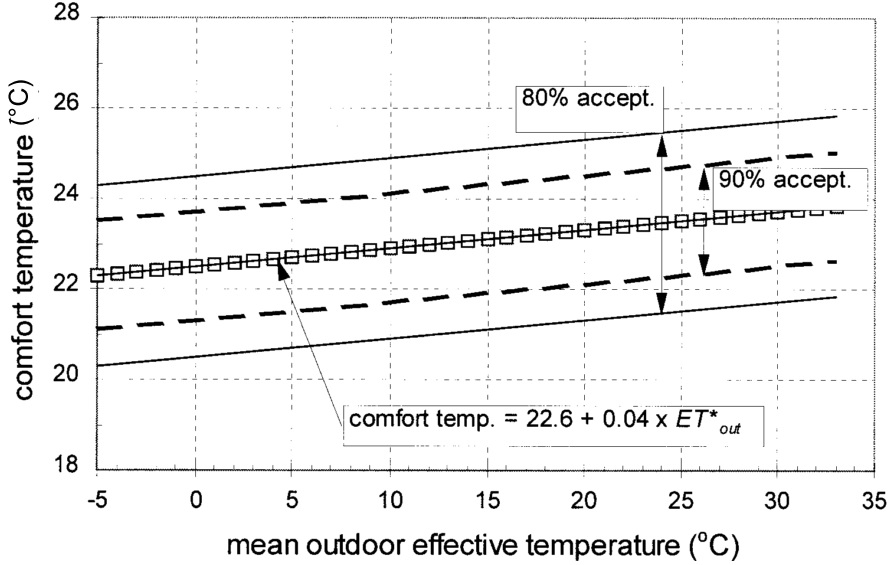
\includegraphics[width=3.2in,keepaspectratio]{./figs/dear_adaptive_thermal_model.jpg}
\caption{Adaptive comfort model for buildings with centralized HVAC and non-opening windows adapted from \cite{de1998developing}}
\label{fig:background:dear_adaptive_temp}
\end{figure}

The adaptive comfort model defines a variable temperature setpoint based on the effective temperature (ET), which is calculated based on the arithmetic average of outdoor temperature at 6 a.m. (assumed minimum daily temperature) and outdoor temperature at 3 p.m. (assumed maximum daily temperature) for a calendar month or particular days. Contrary to the static assumptions underlying the PMV method in \cite{fanger1970thermal}, their results show that occupants thermal comfort sensations are impacted by outdoor temperature, as shown in Figure \ref{fig:background:dear_adaptive_temp}. Based on this finding, numerous studies have been conducted and showed that the adaptive model leads to substantial energy reductions \citep{mui2003adaptive,egan2010the,ward2010automate,yang2013development,west2014trial,chew2015adaptive}. Adopting the adaptive model is a matter of actively managing occupant expectations influencing comfort perception and promoting thermal acceptability \citep{ward2010automate}. In Chapter \ref{cha:atc}, we present a model that allows the occupant to indicate their thermal comfort flexibility. Based on this input, we demonstrate substantial energy savings by dynamically adjusting the comfort setpoints, while providing probabilistic guarantees of thermal comfort satisfaction, considering the uncertainty in the thermal flexibility of occupants.


 
%Each countries define different standards that provide minimum requirements for acceptable indoor thermal environments \citep{vic2008workplace}.
%These standards establish the ranges of indoor environmental conditions that are acceptable to achieve thermal comfort for occupants. 
%In the US, 
%Alternately, in Australia, the optimum comfort temperature for sedentary work is defined between 20$^\circ$C and 26$^\circ$C, depending on the time of the year and clothing worn \citep{vic2008workplace}. 
%While different countries have different standards, each geographical location may account for a spread of a few degrees from the standard indoor temperatures defined above. 
%In commercial buildings, the indoor climate to be maintained is a compromise between those necessary to ensure the comfort of occupants and those necessary to avoid high operating cost due to the energy consumption. A comfort room temperature is essential to assure occupants' productivity. Studies show that productivity drops by 20\% when the employees feel either too hot or too cold in the office environment \citep{}. 



% Add step of MIP like LNS
%
% Give a picture of MIP procedure
%										LNS destroy and repair
%										Online receding horizon
%										Robust control and scheduling

\chapter{Background - Optimisation}
\label{cha:opt}

This chapter provides a brief background of the optimisation techniques applied in this thesis. These include mixed integer programming (MIP), large neighbourhood search (LNS), online optimisation and robust optimisation. We give a fundamental overview and introduce the basic idea of each technique. We explain these techniques in chronological order following their applications to our integrated HVAC control and occupancy scheduling model. Section \ref{sec:mip:concept} describes MIP. Section \ref{sec:lns:concept} introduces LNS,  followed by online optimisation in Section \ref{sec:online:concept}. Finally, Section \ref{sec:atc:robust_opt:concept} covers robust optimisation. 
%This chapter is intended to give a fundamental overview of each technique for readers that are not familiar with the topics. 
All of these approaches have been widely studied, and an exhaustive literature review is beyond the scope of this work. 
We refer readers who are interested for more detailed elaborations to the cited papers. 

\section{Mixed Integer Programming}\label{sec:mip:concept}
% http://www.gurobi.com/resources/getting-started/mip-basics
% http://www.mcs.anl.gov/papers/P3060-1112.pdf
% http://www.gamsworld.org/minlp/siagopt.pdf
%  https://resources.mpi-inf.mpg.de/conferences/adfocs-03/Slides/Rothberg_1.pdf

Our work is fundamentally formulated using mixed-integer programming (MIP) model. A MIP model is an optimisation problem of the form
\begingroup
\begin{align*}
\mbox{minimise:} \quad &c^Tx	\\
\mbox{subject to} \quad &Ax = u	\quad \mbox{(linear constraints)} \\
&\undersl{x} \leq x \leq \oversl{x}	\quad \mbox{(bound constraints)}\\
\mbox{\emph{some or all }} &x_i \mbox{\emph{ must take integer values} \quad (integrality constraints)}
\end{align*}
\endgroup

\noindent where $A$ is an $m \times n$ constraint matrix, $x$ is a vector of $n$ variables, $c$ is the objective function, $\undersl{x}$ and $\oversl{x}$ are vectors of bounds. Some of the variables in vector $x$ are constrained to be integers, while other variables are allowed to be non-integers. Thus, a MIP is a linear program with an integrality restriction on some or all of the variables \citep{bixby2000mip}. The integrality constraints allow MIP models to capture the discrete nature of some decisions. For example, a binary variable $x_{l}$ whose values are restricted to 0 or 1, can be used to decide whether or not an action is taken, such as scheduling an activity or activating the HVAC in location $l$. 

The above model is a mixed integer linear program as it has a linear objective and sets of linear constraints. The following shows a more complicated mixed integer non-linear program (MINLP) model that we tackle in Chapter \ref{cha:milp}:

%\begingroup
%\begin{align*}
%\mbox{minimise:} \quad &x^TQy + c^Tx + b^Ty	\\
%\mbox{subject to} \quad &Az = u	\quad \mbox{(linear constraints)} \\
%&x^TQy + c^Tx + b^Ty = v	\quad \mbox{(bilinear constraints)} \\
%&\undersl{x} \leq x \leq \oversl{x}	\quad \mbox{(bound constraints)}\\
%&\undersl{y} \leq y \leq \oversl{y}	\quad \mbox{(bound constraints)}\\
%&x \in \mathbb{R}^+, y \in \mathbb{R}^+, 	\\
%&z \in \left[0, 1\right] \quad \mbox{(integrality constraints)} \\
%\end{align*}
%\endgroup 

\begingroup
\begin{align*}
\mbox{minimise:} \quad &x^TQy + c^Tx	\\
\mbox{subject to} \quad &w = u + x^TQy\quad \mbox{(bilinear constraints)} \\
&\undersl{w}z \leq w \leq \oversl{w}z	\quad \mbox{(bound constraints)}\\
&\undersl{x} \leq x \leq \oversl{x}	\quad \mbox{(bound constraints)}\\
&\undersl{y} \leq y \leq \oversl{y}	\quad \mbox{(bound constraints)}\\
&w \in \mathbb{R}, x \in \mathbb{R}^+, y \in \mathbb{R}^+ \\
&z \in \left\{0, 1\right\} \quad \mbox{(integrality constraints)} \\
\end{align*}
\endgroup 
\noindent where $x$, $y$ and $z$ are the decision variables, $u$ and $w$ are auxiliary variables, $x$ and $c \in \mathbb{R}^n$, $y \in \mathbb{R}^m$, and $Q$ is a matrix of dimension $n \times m$. $z$ is a vector of binary variables, whereas $x$ and $y$ are sets of positive continuous variables. $\undersl{w}$, $\oversl{w}$, $\undersl{x}$, $\oversl{x}$, $\undersl{y}$, $\oversl{y}$, $\undersl{z}$ and $\oversl{z}$ are vectors of bounds. This model captures the nature of our problem, where $x$ and $y$ denote the interdependent continuous variables in HVAC control and $z$ denotes the discrete scheduling decisions. 

It is easy to see that this is a MINLP problem with a bilinear objective, sets of linear and bilinear constraints, and sets of discrete and continuous decision variables. The matrix $Q$ is not positive semidefinite, so this problem is nonconvex even when the integrality constraints are relaxed. Problems of this type are very difficult to solve, because they combine all the difficulties of both of their subclasses: the combinatorial nature of MIP and the difficulty in solving nonconvex non-linear programs (NLP) \citep{bussieck2003mixed}. Fortunately, innovative approaches and related techniques have been developed to exploit the structure of MIP and NLP within MINLP. 

One approach to solving nonconvex MINLP is to obtain convex relaxations by exploiting the structure of the problem, and solve the corresponding approximation by using mixed-integer linear programming solvers, such as \cite{gurobi}, that are guaranteed to return a lower bound on the globally optimal MINLP objective. To obtain a suitable MILP, we use the linear programming relaxation of bilinear terms introduced by \cite{mccormick1976computability}. This relaxation introduces a new variable $v$ for the bilinear term $xy$ together with four inequalities that define its convex envelope using the bounds $[\underline{x},\overline{x}]$ and $[\underline{y},\overline{y}]$ on each of the two variables involved:

\[\begin{array}{l}
v \geq \underline{x}y + \underline{y}x - \underline{x}\underline{y}\\
v \geq \overline{x}y + \overline{y}x - \overline{x}\overline{y}\\
v \leq \underline{x}y + \overline{y}x - \underline{x}\overline{y}\\
v \leq \overline{x}y + \underline{y}x - \overline{x}\underline{y}
\end{array}
\]
We refer to \cite{belotti2013mixed} for a comprehensive survey of the state-of-the-art methods for solving this challenging class of problems.

MILP problems are generally solved using LP-based branch-and-bound algorithm, or more specifically, \textsl{branch-and-cut}. This algorithm starts by solving the LP relaxation, obtained by simply removing all integrality restrictions. If the solution of this LP model satisfies all the integrality constraints, without them being explicitly imposed, then we can stop. We have found an optimal solution of the original MILP. Otherwise, some integrality restrictions are violated. We then pick an integral variable whose value in the LP relaxation is fractional. Suppose this variable is $x$ with a value of 0.7, we branch and create two new sub-MIP problems, one of which has the added restriction $x \geq 1$ and the other of which has the added restriction $x \leq 0$. If we can compute optimal solutions for each of these two sub-MIP problems then we can take the better of these two solutions and replace the original MIP. Upon identifying the optimal integral value for variable $x$, we have identified a cutting plane that cuts off the solution to the current LP, and we can now add the more restricted integral constraints to the original MIP. The procedure is repeated. If it happens that all of the integrality restrictions in the original MIP are satisfied in the solution, then we know that we have found a feasible solution to the original MIP. 

Two important values are generated during the branching process: an upper bound objective function that is obtained by finding feasible integral solutions, and a lower bound objective function that is obtained from the LP relaxation amongst all active branch-and-cut MIP sub-problems. The difference between the current upper and lower bounds is known as the gap. When the gap is zero, an optimal MIP solution is found. %we have demonstrated optimality. 
As a side note, presolve, cutting planes, heuristics and parallelism are four important procedures that improve on the efficiency of MIP algorithms. We refer to \cite{gurobi16mip} for an in-depth primer about MIP.


\section{Large Neighbourhood Search}\label{sec:lns:concept}

To scale our work to a larger problem size such as university timetabling, and meeting scheduling for commercial offices with huge number of rooms, we employ large neigbourhood search (LNS) in Chapter \ref{cha:lns}. LNS \citep{shaw1998using} is a hybrid optimisation technique that combines MIP or constraint programming (CP) \citep{rossi2006handbook,hentenryck2009constraint} with local search (LS). Traditionally, local search is a heuristic search paradigm that moves from one configuration to the next based on local moves without pruning the search space nor extending partial solutions. It attempts to solve optimisation problems within reasonable time constraints without offering any optimality guarantees. In contrast, MIP and CP are optimisation techniques that are very good at finding optimal solutions but they fail to scale when the model involves a lot of variables. LNS tries to get the best of both methods: exploring the solution space and escaping local minima using local search, and exploiting the power of tree pruning and finding optimal solutions for a smaller sub-problems using MIP/CP.

\newpage
LNS solves a global optimisation problem by dividing them into many smaller problems and solve them to its optimality. It consists of four steps:
\begin{enumerate}
	\item start with a feasible solution,
	\item select a neighbourhood,
	\item re-optimise the neighbourhood using MIP/CP,
	\item repeat the steps, or exit.
\end{enumerate}

The first step consists of finding a feasible solution to the global problem. This is usually obtained by using MIP or CP as they are very good at finding feasible solutions. The key ideas of LNS lie in the second and third steps. The first key idea is to define its neighbourhood by fixing a subset of variables to their values in the best solution found so far and releasing the rest of the variables. We call this the \textsl{destroy} step. As the number of variables released at a time are usually larger than typical local search moves, one cannot rely on enumeration or simple heuristics, the so-defined neighbourhoods require a powerful algorithm to be explored \citep{danna2003structured}. Hence, the second key idea is to create several sub-problems and optimise these using MIP or CP. These sub-problems are constrained by the fixed partial solutions, but are free to re-optimise the destroyed part. We call this the \textsl{repair} step. As CP and MIP are good at pruning the search space, these methods are capable of finding better solutions within a short period of time. The final step involves repeating the procedure or exiting the procedure when a stopping criterion, such as time limit or run limit is met. This hybrid model allows us to easily navigate through the solution space whilst solving difficult core sub-problems to near-optimality. 

One essential question of LNS is how to define a neighbourhood, that is which variables to free simultaneously in order to yield a better solution further away from the current solution. The basic intuition is to release variables which are correlated because they allow each other to change values and lead to a better solution. This can be achieved by exploiting the structure of the problem, or leveraging domain-specific knowledge. It is common for different problems to have different type of neighbourhoods. For example, in a job-shop scheduling problem, the neighbourhoods are formed by sets of machines, whereas for a vehicle routing problem, the neigbourhoods are formed by sets of vehicles. The neighbourhoods can be defined using the following schemes \citep{danna2003structured}:
\begin{itemize}
	\item a \textsl{random neighbourhood} that releases randomly chosen activities/jobs assigned to a room, a machine or a vehicle,
	\item a \textsl{resource-based neighbourhood} that releases all activities on given resources, eg. all activities assigned to a room, all jobs assigned to a machine or a vehicle,
	\item a \textsl{random time window neighbourhood} that releases activities scheduled within different time windows on different resources, eg. all activities assigned to room A on Monday and to room B on Friday, all jobs assigned to vehicle A and B on Tuesday and Thursday, all tasks assigned to machine A, B and C during morning shift.
	\item a \textsl{consecutive pair neighbourhood} that releases pairs of consecutive activities, eg. activities that are scheduled in the same room one after the other.	
\end{itemize}

Note that this is a non-exhaustive list of the possible neighbourhoods that can be built. More variety of neighbourhoods can be formed by taking advantage of different properties of the problem model. For example, in a job shop scheduling problem, it is also possible to construct a neighbourhood which releases a number of jobs that are not scheduled on time, with an aim to minimise its earliness/tardiness cost. % objective function.
Moreover, the abovementioned neighbourhood selection schemes rely heavily on randomization. There are some other schemes that combine LNS with tabu search \citep{abdullah2007tabu}, token-ring search \citep{di2002multi}, or stochastic roulette wheel search \citep{pisinger2007general} to decide on the selection of neighbourhoods.

%The essential question of LNS: how to define neighbourhood - example - to free related variables..
%What is the neighbourhood?
%fix a subset of variables to their values in the best solution found so far
%which subset
%	- problem specific
%	- exploit the problem structure
%leverage on structure of the problem, take advantage of different properties of the problem model
%leverage on the structure of MIP model

Another important criteria in LNS is deciding the size of neighbourhood. For efficiency, it is intuitive to construct a small neighbourhood so that maximum yield is obtained by destroying a small set of variables. This also increases the number of destroy and repair steps that can be executed within a certain time limit, with an aim to further improve the results using smaller sub-problems. On the other hand, it is also necessary to construct a larger neighbourhood to diversify the search, especially when LNS could not improve on the results in smaller neighbourhoods. Another crucial decision is whether the repair step should be optimal or not. When the sub-problems are too large, CP or MIP may take very long to solve them to optimality. In this case, it is possible to truncate the tree search using a fixed or adaptive time limit, node limit or discrepancy limit.

Parameter tuning on the LNS parameters such as (a) randomness of choice in neighbourhood selections, (b) variable of size in the destroy sets, and (c) runtime limit/node limit/discrepancy limit in the repair step are essential in achieving good LNS performance overall. There are numerous values that these parameters can take on. In order to identify the best configurations, a number of automated parameter tuning tools have been developed and used to tune these parameters \citep{hutter2011sequential,malitsky2013tuning}.


%a local search paradigm that makes moves like local search, but uses a tree-based search, such as constraint programming or mixed integer programming, to identify optimal feasible solution within smaller neighbourhoods \citep{shaw1998using}. 
%It involves multiple iterations of destroy and repair steps to identify good or near-optimal solutions. 

%destroy - fix variable, release other, because variables is alot, tree search algoritm is required
%repair - CP propagation and heuristics or MIP branch and cut
%Give example
% Local methods attempts to solve optimisation problems without offering any optimality guarantees. 
% When considering discrete variables, methods producing feasible solutions mainly rely on local search methods.

% http://www.ferc.gov/CalendarFiles/20120627085931-Wednesday_SessionA_Rothberg.pdf
% https://www-304.ibm.com/support/docview.wss?uid=swg21400016 - breaking symmetry

%Symmetry can occur when a model contains groups of integer variables that are all quite similar. When the CPLEX branch and cut algorithm encounters one such variable at a fractional value and branches on it, the algorithm can simply transfer the fractional value of the branching variable to another variable in the group. For example, suppose we have 5 trucks with identical capacities and costs in our model, and xij corresponds to a binary decision variable for assigning truck i to route j for i = 1,...,5. If x1j = .5 and xij = 0 for i = 2,...,5 in the initial LP relaxation of the CPLEX MIP algorithm, then branching down on x1j will probably result in a solution of x2j = .5 and xij = 0 for i = 1,3,4,5 in the next LP subproblem. No useful branching has happened; the fractional value has simply moved from one truck to another identical one, and the process could repeat itself 3 more times in this model. However, since the trucks are identical in terms of the characteristics being modelled, we really don't care which truck gets assigned first. So, we might as well add a constraint that orders the assignment of these trucks:
%x1j >= x2j >= x3j >= x4j >= x5j
%This constraint won't tighten the bound on the best possible integer solution, but it will make sure that truck i is always dispatched before truck i+1, thus preventing unnecessary branches that would arise by swapping identical trucks.
%Symmetry breaking constraints like the one described here are the easiest way to remove performance problems of this type. However, in some cases, you may need actually to reformulate the model to remove symmetry. For a discussion of model reformulation to avoid symmetry, read this file Rethinking Mixed Integer Model Formulations.doc
%Rethinking Mixed Integer Model Formulations.doc
%or click here for an article about this topic.
%Starting with version 8.0, CPLEX includes a symmetry detection parameter to automatically detect certain types of symmetry in MIP models, including the symmetry in the trucking example above. Additional symmetry detection capabilities, controlled by higher values of this parameter, were added with more recent versions. If you suspect symmetry is a source of slow performance for your MIP, try setting this parameter to its highest value. If that doesn't yield the desired performance improvements, then consider the addition of symmetry breaking constraints or alternate model formulation approaches described in this technote.


\section{Online Optimisation} \label{sec:online:concept}

% http://www.aaai.org/Papers/ICAPS/2006/ICAPS06-023.pdf
% http://www.nt.ntnu.no/users/skoge/prost/proceedings/ecc-2013/data/papers/0291.pdf

% By reducing the problem to its minimal structure, one can hope to attain the intrinsic difficulty of learning. 

%\textcolor[rgb]{1,0,0}{Say Solve complex problem by dividing into temporal problems? }
%\textcolor[rgb]{1,0,0}{Online scheduling - we do not predict future events, but with online MPC - we do take in considerations of future dynamics. Greedy with respect to future meeting request, but we predict future events such as changes in weather}

Online optimisation deals with the optimisation problems having no or incomplete knowledge of the future \citep{jaillet2012online}. In many situations, present decisions need to be made with only partial knowledge of the upcoming events. In such cases, online optimisation can be used. This is orthogonal from stochastic optimisation and Markov Decision Processes which rely on statistical distributions. The latter approaches observe a sequence of events, form probability distributions and make decisions taking into considerations the possible occurrence of future events. Whilst it is possible to use probability distributions to inform online decisions \citep{hentenryck2009online}, it is also possible to formulate an online optimisation model which makes no probabilistic assumption on the future \citep{bubeck2011introduction}. 

Online optimisation has been applied in a range of problem types, which include the scheduling of complex transportation and logistic systems \citep{golden2008vehicle}, optimising financial investment problems \citep{mulvey2004financial}, manufacturing production problems \citep{hatono1991modeling} and cyber-physical system control problems in near-real time \citep{wang2010fast,jost2013accelerating}. In our work, we introduce an online integrated HVAC control and occupancy scheduling approach in Chapter \ref{cha:online} to cope with dynamically arriving activity requests while continuously improve on the HVAC control. 

The following shows an online MILP model that we tackle in Chapter \ref{cha:online}. In the online model, the scheduler runs recurrently and each run is called an \emph{online session}. Each online session $i\in I$ starts at time $\tau_i$ and ends before the next session starts at time $\tau_{i+1}$. The following shows a formalisation of an online mixed integer linear programming model that we tackle in Chapter \ref{cha:online}. We adopt a discrete-time linear model, in which the model discretizes time into a set K of time steps. Each time step $k\in K$ starts at time $t_{k}$, and the next time step $k+1$ is separated by a fixed duration $t_{k+1}-t_{k} = \bm{\Delta_t} \in \mathbb{R}^+$. Each on-line session $i$ considers a horizon of $n$ time steps $K(i) = \{k(i), \ldots, k(i)+n-1\}$ where $k(i)$, the first time step in that horizon, is the least time step in $K$ such that $t_{k(i)} \geq \tau_i$. 
\begingroup
\begin{align*}
\mbox{minimise:} \quad &v_k + c^Tx_k	\\
\mbox{subject to} \quad &w_k = u_k + v_k \quad \forall k \in K(i) \\
&\undersl{w}z_k \leq w_k \leq \oversl{w}z_k	\quad \forall k \in K(i) \\
&\undersl{x} \leq x_k \leq \oversl{x}	\quad \forall k \in K(i) \\
&\undersl{y} \leq y_k \leq \oversl{y}	\quad \forall k \in K(i) \\
&v_k \geq \underline{x}y_k + \underline{y}x_k - \underline{x}\underline{y} \quad \forall k \in K(i) \\
&v_k \geq \overline{x}y_k + \overline{y}x_k - \overline{x}\overline{y} \quad \forall k \in K(i) \\
&v_k \leq \underline{x}y_k + \overline{y}x_k - \underline{x}\overline{y} \quad \forall k \in K(i) \\
&v_k \leq \overline{x}y_k + \underline{y}x_k - \overline{x}\underline{y} \quad \forall k \in K(i) \\
&w \in \mathbb{R}, x \in \mathbb{R}^+, y \in \mathbb{R}^+ \\
&z \in \left\{0, 1\right\} \\
\end{align*}
\endgroup 
Similarly to the model in Section \ref{sec:mip:concept}, $x$, $y$ and $z$ are the decision variables, $u$ and $w$ are auxiliary variables, $x \in \mathbb{R}^n$, $c \in \mathbb{R}^n$ and $y \in \mathbb{R}^m$. $z$ is a vector of binary variables, whereas $x$ and $y$ are a vector of positive continuous variables, respectively. $\undersl{w}$, $\oversl{w}$, $\undersl{x}$, $\oversl{x}$, $\undersl{y}$, $\oversl{y}$, $\undersl{z}$ and $\oversl{z}$ are vectors of bounds. $v$ is a new variable introduced for the bilinear term $xy$ together with four inequalities that define its convex envelope using the bounds $[\underline{x},\overline{x}]$ and $[\underline{y},\overline{y}]$ on each of the two variables involved.

In our joint model, we tackle both online scheduling and online MPC in parallel. 

%Online scheduling is a variant in the online optimisation paradigm we tackle. 
In online scheduling, schedules are incrementally updated upon receiving an event or a batch of events within a short interval of time. These schedules are evaluated as a function of the time and resources allocated (eg. number of activities assigned and energy used etc.) and the goal is to maximise the overall quality of actions executed over a finite-receding horizon \citep{gallagher2006incremental}. Online scheduling problems are generally constrained by deadlines and resource availability. Usually, the solution quality of an online schedule is worse than that of the full-knowledge offline solution. Thus, the solution algorithm is often evaluated by the ability to handle dynamically arriving requests with different level of constrainedness, such as deadline, time window, location and other resource flexibilities, whilst preserving the solution quality. 

%Online MPC is a online control mechanism we consider. 
As discussed in Chapter \ref{cha:background}, MPC is a receding-horizon control mechanism that optimises the current time slot while keeping future events in account. This is achieved by optimising over a finite time-horizon given inputs for future time steps, but only implementing the decisions relating to the current time slot. \textsl{Online} MPC solves an MPC control optimisation problem in every online session, usually due to perturbations from external factors such as system interruption or event triggered that require an update to the control problem. Since a constrained optimisation problem has to be solved in every time step, the online computational effort of MPC is high. Research has been conducted to accelerate online MPC by exploiting the structure of the problem \citep{wang2010fast,lim2016online}, or by warm-starting the problem with partial solutions \citep{jost2013accelerating}.

The issue of incomplete data is an essential aspect of online optimisation. How well an online algorithm can perform and how one can guarantee solution quality even without knowing all data in advance are the primary challenges of the online optimisation methodology \citep{jaillet2012online}. In our scheduling approach, we do not predict future events, but with online MPC, we do take the future dynamics into consideration. Our model is greedy with respect to scheduling future meeting requests, but we predict future events such as changes in weather. One advantage of this approach is that it can divide complex problem into multiple temporal problems, and solve them quickly given a relatively smaller problem size compared to the offline approach. In our case, this approach reduces the problem size of our integrated model and produces a solution in a timely manner.


\section{Robust Optimisation} \label{sec:atc:robust_opt:concept}

Robust optimisation is used in Chapter \ref{cha:atc} to enable adaptive temperature control. 
This optimisation paradigm deals with models featuring parameters taking values in a given uncertainty set \citep{bertsimas2011theory}. 
Instead of seeking to immunize the solution in some probabilistic sense to stochastic uncertainty, a robust model is constructed to provide some guarantee of solution quality or feasibility for any realization of the \textsl{uncertainty in a given set}. Under this approach, a certain measure of robustness is sought with respect to the uncertainty set, with an aim to derive feasible and near optimal solutions under some trade-off of constraint violations. Unlike stochastic optimisation, this paradigm can be computationally tractable and does not suffer from the curse of dimensionality. 

Given an objective function to optimise subject to constraints with uncertain parameters, the general robust optimisation formulation \citep{bertsimas2011theory} is 

\begingroup
\begin{align*}
\mbox{minimise:} \quad &c^Tx	\\
\mbox{subject to} \quad &Ax \leq b \quad \forall x \in \mathbb{R}^n, a_1 \in U_1, \ldots, a_m \in U_m.
\end{align*}
\endgroup

\noindent Here, $a_i$ represents the $i$th row of the uncertain matrix $A$ and elements in $a_i$ are assumed to take arbitrary values in the uncertainty set $U_i \subseteq \mathbb{R}^n$. The goal is to compute minimum cost solutions $x^\ast$ among all feasible solutions and for all realizations of the parameters $a_i$ within $U_i$. Note that $a^T_i x \leq b_i \quad \forall a_i \in U_i$ if and only if $max_{\left\{a_i \in U_i\right\}} a_i^Tx \leq b_i \quad \forall i$ (i.e. worst case protection). Intuitively, this approach offers some measure of feasibility guarantees for optimisation problems featuring parameters with unknown values. More specifically, this protection is achieved by enforcing \textsl{hard constraints} given a \textsl{prescribed} uncertainty set $U_i$. 

In our work, we focus on a specific class of robust optimisation problems that consider ellipsoidal uncertainty sets proposed by \cite{BenT99,ben2000robust}. This approach allows us to control the level of robustness by defining restrictions on the uncertainty set $U_i$, and to trade-off between feasibility and optimality. %robustness and performance. 

An uncertainty set $U_i$ is defined as
\begingroup
\begin{align*}
%U_i = \left\{\left(a_1,\ldots,a_m\right): a_{i,j} = \bar{a}_{i,j} + \hat{a}_{i,j} \xi_{i,j}, \quad \forall j \in \left\{1,\ldots,k\right\}, \quad \left\|\xi_i\right\|_\infty \leq 1, \left\|\xi_i\right\|_2 \leq \delta\right\}
U_i = \left\{a_i \in \mathbb{R}^n | a_{i,j} = \bar{a}_{i,j} + \hat{a}_{i,j} \xi_{i,j}, \quad \forall j \in \left\{1,\ldots,n\right\}, \left\|\xi_i\right\|_\infty \leq 1, \left\|\xi_i\right\|_2 \leq \delta\right\}
\end{align*}
\endgroup

\noindent where $\bar{a}_i$ denotes a vector of nominal values, $\hat{a}_i$ denotes a vector of deviation values and $\xi_i \in \mathbb{R}^n$ denotes a vector of independent and uniformly distributed random variables corresponding to the $i$th constraint, taking values in $\left[-1, 1\right]$. 

The advantage of considering uncertainty set $U_i$ lies in the constraint satisfaction guarantee. \cite{ben2000robust} shows that if the uncertainty sets are bounded by ellipsoids of radius $\delta$, the corresponding feasible solutions have a constraint satisfaction probability that is linked to $\delta$. 

\cite{babonneau2009robust} defines a robust counterpart of the above robust formulation by introducing variables $y, w \in \mathbb{R}$ and proves that the robust solution satisfies the constraint with probability at least $1-e^{-\delta^2/2}$:
\begingroup
\begin{align*}
\mbox{minimise:} \quad &c^Tx	\\
\mbox{subject to} \quad &\bar{a}_i^Tx + \left|\hat{a_i}\right|^Ty + \delta \sqrt{\left(\hat{a_i}^2\right)^T w^2}  \leq b_i  \quad \forall i = 1,\ldots,m. \\
&-y \leq x-w \leq y \\
&y \geq 0
\end{align*}
\endgroup

\cite{hijazi2013robust} considers a special case where the uncertain coefficients are independent from the model variables. They consider a vector $a_i$ of random variables that capture the uncertainties, where each vector element $a_{i,j}$ takes it value in the given range $\left[\bar{a}_{i,j} - \hat{a}_{i,j}, \bar{a}_{i,j} + \hat{a}_{i,j}\right]$. % and the sum of vector elements brings an uncertain parameter disturbing the constraint satisfaction. 
They prove that the model proposed by \cite{babonneau2009robust} can be simplified and adapted for this special case as follows:

\begingroup
\begin{align*}
\mbox{minimise:} \quad &c^Tx	\\
\mbox{subject to} \quad &h(x) + \bar{a}_i^T + \hat{a_i}^T \mathbb{1}^S + \sqrt{\left(\delta^2 - \left|S\right|\right) \left(\hat{a}_i^2\right)^T \mathbb{1}^{\bar{S}}}  \leq b_i  
\end{align*}
\endgroup

\noindent where $\mathcal{S}$ is a set of indices corresponding to the offset of elements in vector $a$, determined based on an algoritm described in \cite[Proposition 1.]{hijazi2013robust}. $\mathbb{1}^S$ is a vector of binary elements where each element equals 1 if the element is in the set $\mathcal{S}$, and $\mathbb{1}^{\bar{S}}$ is its complement. Their model is used in a network-based problem where given paths accumulate random delays at each network node. Their approach is applicable to our work where the room temperature bounds can be adjusted at each time slot, according to the unknown occupants' tolerance and outdoor temperature fluctuation, which represents our set of uncertain parameters.%, which\textcolor[rgb]{1,0,0}{ own set of uncertain parameters}.

We refer readers to \citep{Elgh97,BenT98,BenT99,babonneau2009robust,hijazi2013robust} for more detailed theorems and proofs of this approach and to \cite{bertsimas2011theory,gabrel2014recent} for comprehensive surveys of the state-of-the-art theory and applications of robust optimisation. 


%Robust optimisation constitutes a subsection of our work in Chapter \ref{cha:atc} to enable adaptive temperature control. 
%This optimisation paradigm deals with uncertainty in optimisation problems, in which the uncertainty model is not stochastic, but rather deterministic and set-based \citep{bertsimas2011theory}. Instead of seeking to immunize the solution in some probabilistic sense to stochastic uncertainty, a robust model is constructed to provide guarantee of solution quality or feasibility for any realization of the \textsl{uncertainty in a given set}. Under this approach, a certain measure of robustness is sought against the uncertainty set, with an aim to derive feasible and near optimal solution under some trade-off of constraint violations. Unlike stochastic optimisation, this optimisation paradigm is often computationally tractable and does not suffer from the curse of dimensionality. 
%
%Given an objective function to optimise subject to constraints with uncertain parameters, the general robust optimisation formulation \citep{bertsimas2011theory} is 
%
%\begingroup
%\begin{align*}
%\mbox{minimise:} \quad &c^Tx	\\
%\mbox{subject to} \quad &Ax \leq b \quad \forall a_1 \in U_1, \ldots, a_m \in U_m.
%\end{align*}
%\endgroup
%
%\noindent Here, $a_i$ represents the $i$th row of the uncertain matrix $A$ and are assumed to take arbitrary values in the uncertainty set $U_i \subseteq \mathbb{R}^n$. The goal is to compute minimum cost solutions $x^\ast$ among all those solutions which are feasible for all realizations of the disturbances $a_i$ within $U_i$. Note that $a^T_i x \leq b_i \quad \forall a_i \in U_i$ if and only if $max_{\left\{a_i \in U_i\right\}} a_i^Tx \leq b_i \quad \forall i$ (i.e. worst case protection). Intuitively, this problem offers some measure of feasibility protection for optimisation problems containing parameters which are not known exactly. More specifically, this protection is achieved by relaxing \textsl{hard constraints} with a \textsl{prescribed} uncertainty set $U$. 
%
%In our work we focus at specific class of robust optimisation that consider ellipsoidal uncertainty sets proposed by \cite{BenT99,ben2000robust}. This approach allows us to control the level of robustness by defining the restrictions on the uncertainty set $U$, and to trade-off between robustness and performance. 
%
%The uncertainty set $U$ is given as
%\begingroup
%\begin{align*}
%U = \left\{\left(a_1,\ldots,a_m\right): a_i = \bar{a}_i + \hat{a}_i \xi_i, \quad \forall i \in \left\{1,\ldots,m\right\}, \quad \left\|\xi\right\|_\infty \leq 1, \left\|\xi\right\|_2 \leq \delta\right\}
%\end{align*}
%\endgroup
%
%\noindent where $\bar{a}_i$ denotes a vector of nominal values, $\hat{a}_i$ denotes a vector of arbitrary values, that take their values independently and following no specific distribution, and $\xi_i$ denotes a vector of random variables corresponding to $i$th constraint and takes values in $\left[-1, 1\right]$. 
%
%The advantage of considering uncertainty set $U$ lies in the constraint satisfaction guarantee. \cite{ben2000robust} shows that if the uncertain sets are bounded by ellipsoids of radius $\delta$, the corresponding robust feasible solutions have a constraint satisfaction probability that is linked to $\delta$. 
%
%\cite{babonneau2009robust} defines a robust counterpart of the above robust formulation by introducing variables $y, w \in \mathbb{R}$ and proves that the robust solution satisfies the constraint with probability at least $1-e^{-\delta^2/2}$:
%\begingroup
%\begin{align*}
%\mbox{minimise:} \quad &c^Tx	\\
%\mbox{subject to} \quad &\bar{a}_i^Tx + \left|\hat{a_i}\right|^Ty + \delta \sqrt{\left(\hat{a_i}^2\right)^T w^2}  \leq b_i  \quad \forall i = 1,\ldots,m. \\
%&-y \leq x-w \leq y \\
%&y \geq 0
%\end{align*}
%\endgroup
%
%\cite{hijazi2013robust} considers a special case where the uncertain coefficients are independent from the model variables. They consider a vector $a_i$ of random variables that capture the uncertainties, where each vector element $a_{i,j}$ takes it value in the given range $\left[\bar{a}_{i,j} - \hat{a}_{i,j}, \bar{a}_{i,j} + \hat{a}_{i,j}\right]$ and the sum of vector elements brings an uncertain parameter disturbing the constraint satisfaction. They prove that the model proposed by \cite{babonneau2009robust} can be simplified and generalized for this special case as follows:
%
%\begingroup
%\begin{align*}
%\mbox{minimise:} \quad &c^Tx	\\
%\mbox{subject to} \quad &h(x) + \bar{a}_i^T + \hat{a_i}^T \mathbb{1}^S + \sqrt{\left(\delta^2 - \left|S\right|\right) \left(\hat{a}_i^2\right)^T \mathbb{1}^{\bar{S}}}  \leq b_i  
%\end{align*}
%\endgroup
%
%\noindent where $\mathcal{S}$ is a set of indices corresponding to the offset of elements in vector $a$, determined based on a rule-based algoritm described in \cite[Proposition 1.]{hijazi2013robust}. $\mathbb{1}^S$ is a vector of binary elements where each element equals 1 iff the element is in the set $\mathcal{S}$, and $\mathbb{1}^{\bar{S}}$ is its complement. Their model turns out to be applicable for real world problems such as network based problems where the path delay are obtained by summing the disturbance (a.k.a delay) at each network nodes. The same is applicable to our work where the room temperature bounds can be adjusted at each time slot, according to the occupants tolerance and outdoor temperature fluctuation.
%
%We refer readers to \citep{Elgh97,BenT98,BenT99,babonneau2009robust,hijazi2013robust} for more detailed theorem and proofs of this approach and to \cite{bertsimas2011theory,gabrel2014recent} for comprehensive surveys of the state-of-the-art theory and applications of robust optimisation. 

%--------------------
%They introduced a general framework for ellipsoidal uncertainty sets and defined the robust counterpart of corresponding optimisation problems. Based on theorem in \cite{BenT99}, let $U$ be %a set bounded by an ellipsoid of radius $\rho$, i.e.
%\begingroup
%\begin{align*}
%U \equiv U\left(\Pi,Q\right) = \left\{\Pi(u)|\left\|Qu\right\| \leq \delta \right\},
%\end{align*}
%\endgroup
%
%\noindent where $u\rightarrow\Pi(u)$ is an affine embedding of $\mathbb{R}^L$ into $\mathbb{R}^{m\times n}$ and $Q \in \mathbb{R}^{M\times L}$. We can then derive an equivalent second-order cone program (SOCP), 
%
%\begingroup
%\begin{align*}
%\mbox{minimise:} \quad &c^Tx	\\
%\mbox{subject to} \quad &a_ix \leq b_i \quad \forall a_i \in U_i, \forall i = 1,\ldots,m.
%\end{align*}
%\endgroup
%
%\noindent Here, the uncertainty set is given as
%\begingroup
%\begin{align*}
%U = \left\{\left(a_1,\ldots,a_m\right): a_i = \bar{a}_i + \hat{a}_i \xi_i, \quad i=1,\ldots,m, \quad \left\|\xi\right\|_2 \leq \delta\right\}
%%U = \left\{\left(a_1,\ldots,a_m\right): a_i = a^0_i + \Delta_i u_i, \quad i=1,\ldots,m, \quad \left\|u\right\|_2 \leq \rho\right\}
%\end{align*}
%\endgroup
%
%\noindent where $\bar{a}_i $ denotes the nominal value and $\hat{a}_i$ denotes an arbitrary value, independently and following no specific distribution. The robust counterpart is
%
%\begingroup
%\begin{align*}
%\mbox{minimise:} \quad &c^Tx	\\
%\mbox{subject to} \quad &\bar{a}_ix \leq b_i - \delta\left\|\hat{a}_ix\right\|_2   \quad \forall i = 1,\ldots,m.
%%\mbox{subject to} \quad &a^0_ix \leq b_i - \rho\left\|\Delta_ix\right\|_2   \quad \forall i = 1,\ldots,m.
%\end{align*}
%\endgroup
%
%%According to \citep{bertsimas2011theory},
%%The intuition is that, for the case of ellipsoidal uncertainty, the subproblem $\mbox{max}_{\left\{a_i \in U_i\right\}} a_i^T x \leq b_i \quad \forall i$ is an optimisation over a quadratic constraint. The dual, therefore involves quadratic functions which leads to the resulting SOCP. 
%In \cite{ben2000robust}, they further improvised the robust model to provide probability guarantees. Under this model, if the uncertain sets are bounded by the ellipsoids of radius $\delta$, they show that the corresponding robust feasible solutions have a constraint satisfaction probability that is linked to $\delta$. 
%%Specifically, consider a linear constraint $\sum \limits_{j} a_{ij}x_j \leq b_i$, where the coefficients $\tilde{a}_{ij} = (1 + \xi_{ij}) a_{ij}$, where $a_{ij}$ is a nominal value for the coefficient and $\left\{\xi_{ij}\right\}$ are 
%%zero mean, independent over $j$, and supported on $\left[-1, 1\right]$, 
%%independent and symmetrically distributed random variables in $\left[-1, 1\right]$,
%Specifically, consider a linear constraint $\sum_{j} \tilde{a}_{ij}x_j \leq b_i$, where the coefficients $\tilde{a}_{ij}$ are uncertain and given by $\tilde{a}_{ij} = \bar{a}_{ij} + \hat{a}_{ij}\xi_{ij}$, where $\bar{a}_{ij}$ is a nominal value for the coefficient, $\hat{a}_{ij}$ is an arbitrary value follows no distribution and $\left\{\xi_{ij}\right\}$ are independent and symmetrically distributed random variables in $\left[-1, 1\right]$,
%then a robust constraint of the form 
%
%\begingroup
%\begin{align*}
%\sum\limits_{j} \bar{a}_{ij}x_j + \delta \sqrt{\sum\limits_{j} \hat{a}^2_{ij} x^2_j} \leq b_i
%\end{align*}
%\endgroup
%
%\noindent implies the robust solution satisfied the constraint with probability at least $1-e^{-\delta^2/2}$.

%Essentially, the method that we apply enable robust control via robust optimisation technique. 














% TODO:
% 	explain the concept of MIP

%  Add temperature fluctuation at different room based on outdoor temperature..
%  Add full HVAC model and McCormick Model
%  Add example of back-to-back vs. joint model vs. random
%  Add building configuration - say consider building of different type
%  Add related work and non-linear. say hvac non-linear method can be linearised by bla bla hvac linearisation method. Also include related work on hvac using non-linear. Talk about pre-cooling based on meetings
% Future work: say incorporate humidity bla bla bla, refer hassan paper about multilinear term using sequential mccormick, all positive bounds maybe new way of relaxation is possible.

%  The integrated model should achieve higher efficiency in energy reduction by fully exploiting the capability to coordinate through both HVAC control and occupancy scheduling. 

\chapter{Integrating HVAC Control with Occupancy Scheduling}
%\chapter{HVAC-Aware Occupancy Scheduling}
\label{cha:milp}

\section{Introduction}

% TODO:
%  
%  there have been ppl working on occupancy-based HVAC control
% there have been ppl working on energy-aware scheduling
% crystal-cleared about our joint model >> contributions

% One of the main inefficiencies in building management systems is the widespread use of schedule-based control when operating heating, ventilation and air conditioning (HVAC) systems. HVAC systems typically operate on a pre-designed schedule that heats or cools rooms in the building to a set temperature even when rooms are not being used. Occupants, however, influence the thermal behavior of buildings. As a result, using occupancy information for scheduling meetings to occur at specific times and in specific rooms has significant energy savings potential. 

\begin{figure}[bt]
	\centering
		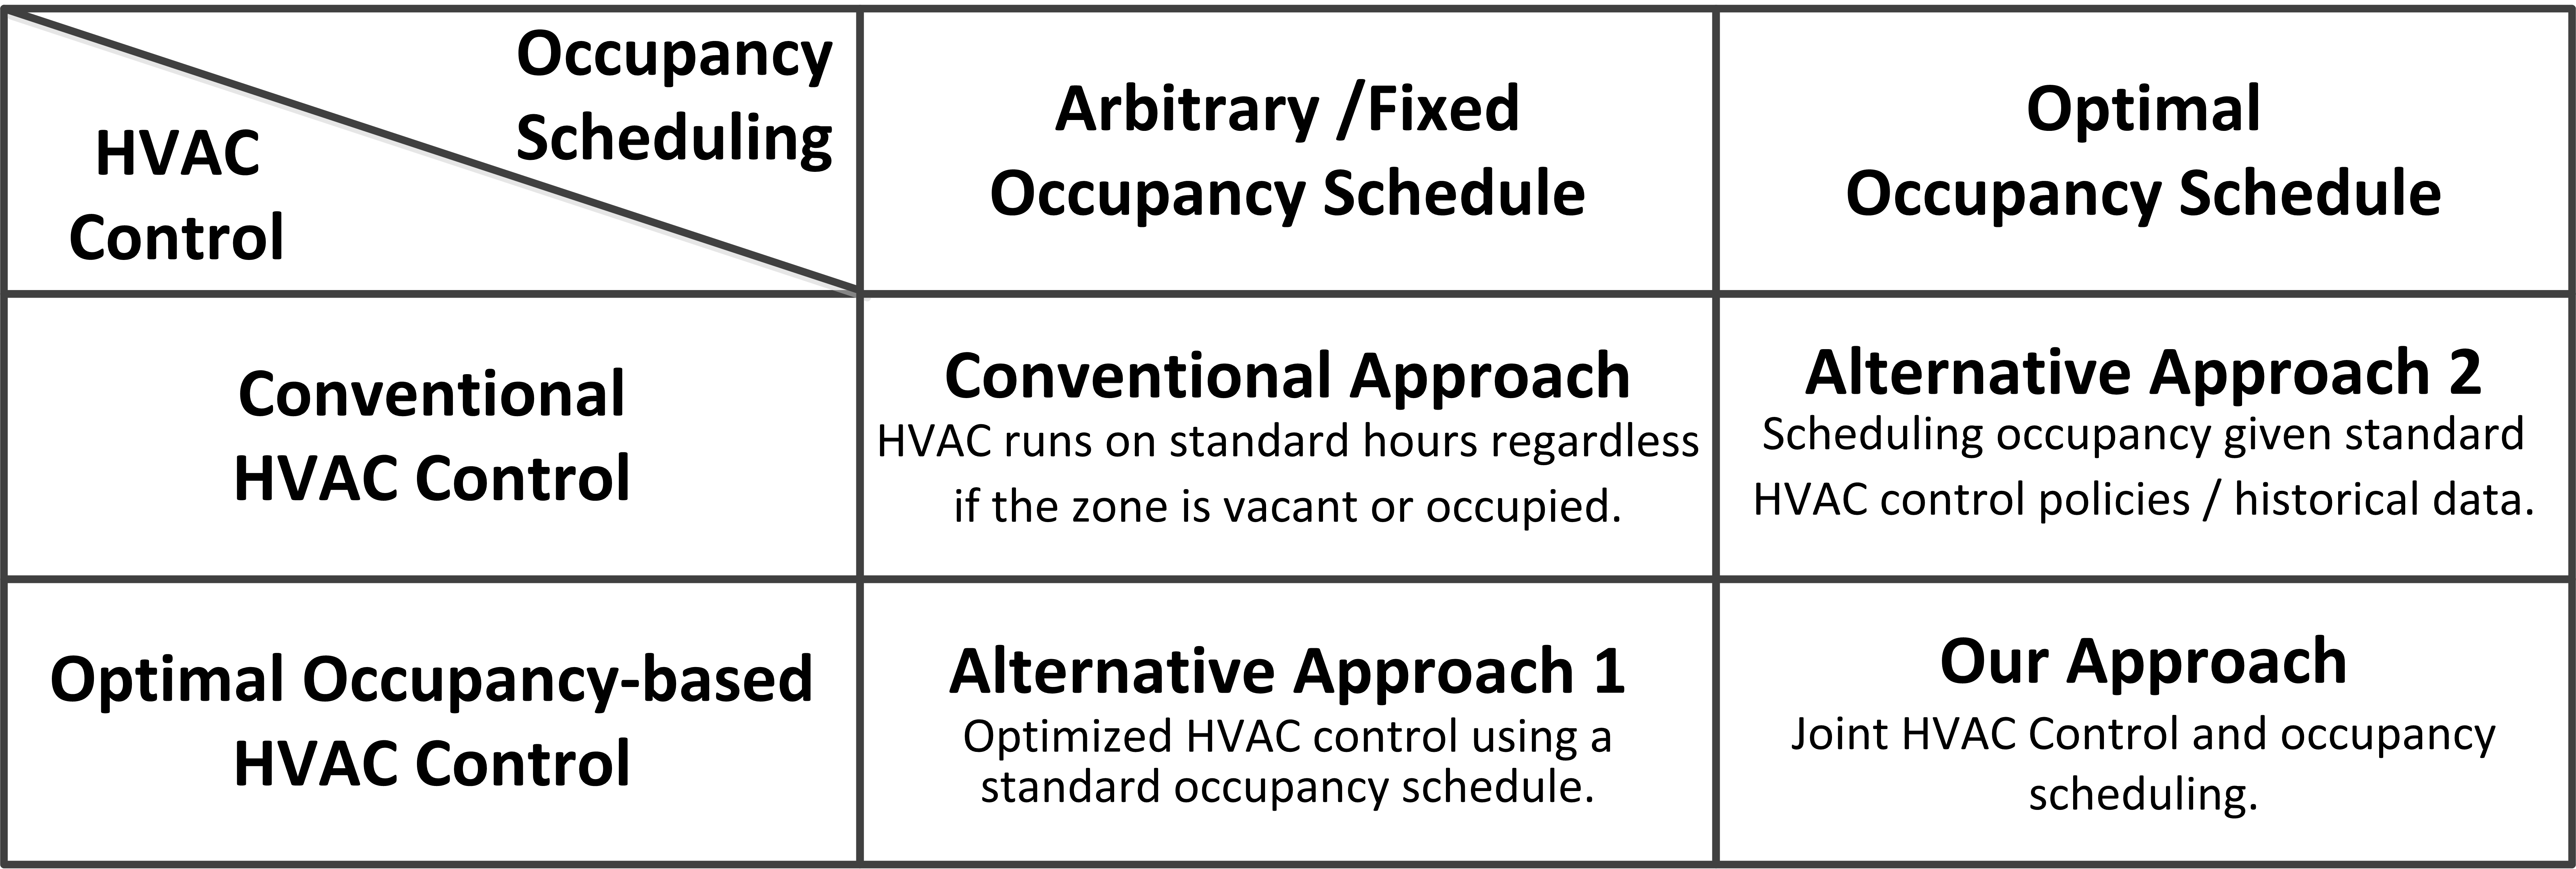
\includegraphics[width=0.74\linewidth,keepaspectratio]{./figs/mip_taxonomy.jpg}		
	\caption{HVAC control \& occupancy scheduling: existing approaches vs. our approach}
	\label{fig:mip_taxonomy}
\end{figure}

Energy consumption in commercial and educational buildings is impacted by group activities such as meetings, workshops, classes and exams.
%Group activities such as meetings, workshops, classes and exams impact the energy consumption in commercial and educational buildings.
Currently, most buildings adopt a conventional approach for managing HVAC systems. The building HVAC is turned on during business hours, typically 6am to 6pm, regardless whether a building zone is occupied or not. This widespread use of fixed schedule-based control constitutes to one of the main inefficiencies in building management system. We believe that energy consumption can be reduced by scheduling group activities to take place at times and locations that are favorable from an energy standpoint.

%As occupants influence the thermal behavior of buildings, 
Various optimisation approaches have been proposed to optimise HVAC utilisation using occupancy information. Figure \ref{fig:mip_taxonomy} shows a simple classification of the existing works on HVAC control and occupancy scheduling, and how our work differs from these state-of-the-art approaches. 

Moving away from the conventional approach, existing works consider only one of the solutions: 
\begin{itemize}
	\item Alternative Approach 1 (Optimal occupancy-based HVAC control-oriented) - The HVAC community focuses at optimising HVAC control using a standard occupancy schedule, or by ``detecting'' if a room is occupied based on sensors \citep{agarwal2010occupancy,goyal2013occupancy,brooks2015energy}. This approach does not perform any occupancy scheduling, and therefore it ignores the fact that there are better schedules that lead to higher energy savings.
	\item Alternative Approach 2 (Optimal occupancy scheduling-oriented) - The scheduling community focuses at optimising the occupancy schedule given standard HVAC control policies or historical data \citep{pan2012thermal,majumdar2012energy,kwak2013tesla,majumdar2016characterising}. They typically adopt suboptimal scheduling strategies guided by heuristics to search for solutions that take advantage of thermal inertia, and schedule activities by considering criteria include minimising the number of rooms used, minimising the time gap between activities in the same room, and minimising the gap between room capacity and the number of occupants.	An important limit of this line of research is that it adopts a black-box modeling approach to calculate HVAC energy consumption, and therefore it fails to exploit the advantage of occupancy HVAC control.
\end{itemize}


%You can do this and do that in sequence, but…. We can do more…. This is what we are doing…
%(after saying sequential step) ……  But (emphasize) we can do something better 

In this chapter, we show that combining HVAC control with occupancy scheduling can lead to substantial improvements in energy efficiency. 
We focus on improving the effectiveness of energy-aware room-booking and meeting scheduling approaches, by allowing the scheduling decisions to rely on an explicit model of the building's occupancy-based HVAC control. The core component of our approach is a mixed-integer linear programming (MILP) model which we use to optimally solve the joint occupancy scheduling and occupancy-based HVAC control problem. This joint problem consists in deciding the respective times and locations of a set of activities, as well as the HVAC supply air flow rate and air flow temperature for each zone and time, in such a way as to optimise the overall HVAC consumption over a receding horizon.

Our initial HVAC control model builds on well-accepted work by \cite{goyal2013occupancy}, but introduces a number of significant changes required to be suitable as a sub-component of our more complex joint scheduling and control model. Notably, the control model studied by \cite{goyal2013occupancy} is a purely continuous {\em non-linear} model which does not consider occupancy. Our experiments, which use the IPOPT solver \citep{Ipopt}, revealed that this model is impractical for our application, in terms of both memory and run-time requirements. In contrast, we formulate an efficient linear model that incorporates discrete variables to capture occupancy. % and after-hour standby mode.
The linear model is formulated by relaxing the non-linear HVAC control constraints in a principled way using McCormick Relaxation \citep{mccormick1976computability}. 

To enable joint optimisation between HVAC control and occupancy scheduling, we introduce a discrete variable that indicates if a location is being occupied by a scheduled activity, which then triggers a HVAC control constraint that ensures the room temperature is between the occupied thermal comfort bound. To ensure the existence of a feasible control for adequately sized HVACs and improve on the current occupancy-based HVAC control practices, we introduce a \textsl{standby mode} enabling the HVAC to re-activate at night if this is necessary to meet the temperature bounds of an early morning meeting or results in reduced consumption. Our experiments illustrate the circumstances under which the standby mode is beneficial, and show the superiority (over 50\% consumption reduction) of our joint MILP model compared to heuristic scheduling solutions and to more na\"{\i}ve integrations of meeting scheduling and occupancy-based HVAC control. 

In the following, we start by introducing the occupancy-based HVAC control aspects of our MILP model in Section \ref{sec:mip:control}. We describe in turn the type of HVAC system we focus on along with the objective function we consider, the bounds the control must comply with, the effect of the control on the building thermal dynamics, and the linear relaxation of the non-linear constraints. In Section \ref{sec:mip:scheduling} we will cover the scheduling aspects and demonstrate how the scheduling model can be integrated to the HVAC control. We provide experimental comparisons of our integrated model with the state-of-the-art in Section \ref{sec:mip:experiments}, followed by a discussion of the related work in Section \ref{sec:mip:related} and finally draw a conclusion in Section \ref{sec:mip:conclusion}. 

%To summarise, the main contributions of the paper are: a) an efficient MILP model for occupancy-based HVAC control which can be used in a range of applications, b) a scalable and effective approach to occupancy scheduling which exploits the capabilities of HVAC control and c) experiments showing a substantial reduction in energy consumption over the state of the art.

\section{Occupancy-Based HVAC Control}
\label{sec:mip:control}

%Following \citep{goyal2013occupancy}, 
We adopt a model predictive control (MPC) approach and consider variable-air-volume (VAV) based HVAC systems, which are widely
deployed in commercial buildings. With such systems, the building is divided into a number of zones (or locations) $L\subseteq\mathbb{N}$,
each of which can be an individual room or a group of rooms. Figure~\ref{fig:hvac} shows a schematic of a VAV system connected to two building zones.  To simplify notation, we assume that each zone corresponds to a
single room. %In the description of the model, values of constants are given between square brackets. 

\subsection{VAV System and Objective Function}
\begin{figure}
	\centering
		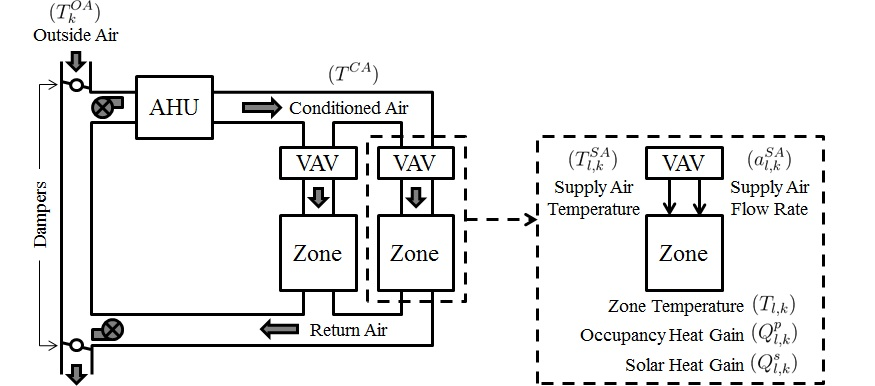
\includegraphics[width=0.74\linewidth,keepaspectratio]{./figs/vav_new.jpg}		
	\caption{VAV-based HVAC system with two zones}
	\label{fig:hvac}
\end{figure}

Let $K = \{1 \ldots n\}$ be a finite set of discrete time steps considered over the optimisation horizon. For simplicity, we assume
that successive time steps are separated by a fixed duration $\bm{\Delta t} \in \mathbb{R}^+$; that is, $\forall k\in K$, we have $t_k \in
\mathbb{R}^+$ and $t_{k} - t_{k-1} = \bm{\Delta t}$. The objective is to minimise the total energy consumed over the optimisation horizon:

\begin{equation} \label{eq:objective}
\mbox{minimise: } \sum_{k\in K} e_{k}
\end{equation}

\noindent where $e_k$ is the energy consumed at time step $k$: 
\begin{equation} \label{eq:e_total} 
e_{k} = p_{k} \times \bm{\Delta t} \hspace{20pt} \forall k \in K 
\end{equation}

\noindent The power $p_{k}$ is consumed by the three main operations shown in Figure~\ref{fig:hvac} and detailed below: the
  air conditioning operation performed centrally by the air handling unit (AHU) consumes $p_{k}^{Cond}$; the fan operation, also
  performed centrally, consumes $p_{k}^{Fan}$; and the reheating operation performed locally at each zone $l\in L$ by the zone's VAV
  unit consumes $p_{l,k}^{Heat}$:
	
\begin{equation} \label{eq:p_total} 
p_{k} = \left( p_{k}^{Cond} + p_{k}^{Fan} + \sum\limits_{l \in L} p_{l,k}^{Heat}\right) \hspace{10pt} \forall k \in K 
\end{equation}

We now provide the details of the power consumed by these 3 operations:

\noindent\emph{Air Conditioning Operation.} The AHU admits a mixture of outside air at temperature $\bm{T^{OA}}_k$ and
return air, and conditions it to a pre-set conditioned air temperature $\bm{T^{CA}}$ [usually $12.8\,^{\circ}\mathrm{C}$]. The conditioned air is then distributed through the supply duct to the VAV unit at each zone. The AHU consumption $p_{k}^{Cond}$ is the power consumed in cooling the total air flow required.  Let $a^{SA}_{l,k}$ denote the air flow rate required by location $l$ at time step $k$ and $\bm{C^{pa}}$ the heat capacity of air at constant pressure [1.005 kJ/kg$\cdot$K]: 

\begin{equation} \label{eq:p_cond}
p_{k}^{Cond} = \bm{C^{pa}}\left(\bm{T^{OA}_{k}} - \bm{T^{CA}}\right) \sum\limits_{l \in L} a_{l,k}^{SA} \hspace{10pt} \forall k \in K 
\end{equation}

\noindent\emph{Fan Operation.} The supply fan, driven by a variable frequency drive, maintains a constant static pressure in the supply
duct. When the opening of the VAV dampers increases to pull in more air flow into the conditioned space (resp. decreases to pull less air
flow), the fan speeds up (resp. slows down). The fan consumption is the power consumed to push the total air flow required through the
supply duct, which is proportional to the sum of the air flow rates $a^{SA}_{l,k}$ required over all locations. Let $\bm \beta$ be the fan
coefficient [0.65]: 

\begin{equation} \label{eq:p_fan}
p_{k}^{Fan} = \bm{\beta} \sum\limits_{l \in L} a_{l,k}^{SA} \hspace{20pt}  \forall k \in K
\end{equation}

\noindent\emph{Reheating Operation.} Each zone $l$ has a VAV unit connected to the supply duct. The unit is equipped with
continuously adjustable valves and reheat coils. These enable regulating the air flow rate $a^{SA}_{l,k}$ into the zone and
modulating the supply air temperature $T^{SA}_{l,k}$ to maintain the zone temperature within given bounds, if necessary by reheating the
supply air. Here we consider the power $p_{l,k}^{Heat}$ consumed by the reheating process to heat the supply air from the conditioned
temperature $\bm{T^{CA}}$ to an appropriate location supply air temperature $T_{l,k}^{SA}$.  

\begin{equation} \label{eq:p_heat} 
p_{l,k}^{Heat} = \bm{C^{pa}} (T_{l,k}^{SA}- \bm{T^{CA}}) a_{l,k}^{SA} \hspace{10pt} \forall l \in L,k \in K 
\end{equation}

\noindent\emph{Decision Variables.} The two key HVAC decision variables are the supply air flow rate $a_{l,k}^{SA}$ and
temperature $T_{l,k}^{SA}$ at each location $l \in L$ and time step $k\in K$. We determine an optimal control for these variables, given
occupancy information and bounds on supply air temperature, supply air flow rate, and room temperature during vacant and occupied
periods. Below we will introduce a third decision variable $w_{l,k}$ to decide when the HVAC should activate at night, which in turn will influence the bounds described below. When taking the HVAC control model in isolation, the building occupancy is an {\em input} to the model. When we integrate scheduling into the model in Section~\ref{sec:mip:scheduling}, occupancy will become a {\em decision variable}.

\subsection{Temperature and Air Flow Bounds}
We now model the constraints on the temperature, supply air temperature and supply air flow rate in each location, as a function
of the location occupancy and the time of the day.  We introduce the auxiliary variable $T_{l,k} \in \mathbb{R}$ representing the {\em
  actual} temperature in location $l\in L$ at time step $k\in K$, and the Boolean input $z_{l,k}$ which is true if and only if $l$ is occupied at time step $k$. When a location is not occupied, its temperature can lie freely within a wide temperature range $[\bm{\underline{T}^{\emptyset}}, \bm{\overline{T}^{\emptyset}}]$, whilst the temperature is otherwise constrained to lie within a more restricted comfort range $[\bm{\underline{T}^{\emptyset}} + \bm{\underline{T}^g}, \bm{\overline{T}^{\emptyset}}-\bm{\overline{T}^g}]$, where $\bm{\underline{T}^g}$ and $\bm{\overline{T}^g}$ are appropriate constants. This constraint is expressed as follows:

\begin{equation} \label{eq:temp_cstr}
\bm{\underline{T}^{\emptyset}} + \bm{\underline{T}^g} z_{l,k} \leq T_{l,k} \leq \bm{\overline{T}^{\emptyset}} - \bm{\overline{T}^g} z_{l,k} \quad \forall l\in L , k \in K 
\end{equation}

Further, the supply air temperature and flow rate at each location are constrained in a way that depends on the HVAC operating mode at the
current time step. We have two operating modes: {\em active} and {\em standby}. Let $K^{s} \subseteq K$ be the set of time steps that fall
within standard operating hours (6am to 6pm).  During standard hours ($k\in K^s$) the HVAC is always in active mode. The supply air
temperature $T^{SA}_{l,k}$ at location $l$ must fall within $[\bm{T^{CA}}, \oversl{\bm{T}}^{SA}]$. The supply air flow rate $a_{l,k}^{SA}$ must fall within $[\bm{\underline{a}^{SA}}_{l}, \bm{\overline{a}^{SA}}]$. The upper bound $\bm{\overline{a}^{SA}}$ [$5.0$ kg/s] is the air flow rate obtained when the dampers are fully open. The lower bound $\bm{\underline{a}^{SA}_l}$ is a constant calculated as a function of the area of the location, the factor of indoor air quality and the return air ratio necessary to ensure that the minimal fresh outside air requirements specified in the ASHRAE ventilation standard are met \citep{ashrae2013thermal}. 

\begin{equation} \label{eq:asalb}
% self.EAMS.ALPHA_IAQ_FACTOR_OF_SAFETY*((self.EAMS.MASS_AIR_FLOW_OUTSIDE_AIR_PER_METER_SQUARE * width * length * height) /
%                                                    (1-self.EAMS.MASS_AIR_FLOW_RETURN_AIR_RATIO))
\bm{\underline{a}_{l}^{SA}} = \bm{\alpha} \times \frac{\bm{a^{OA}} \times \bm{l^{width}} \times \bm{l^{length}}}{1-\bm{a^{RAR}}} \quad \forall l\in L
\end{equation}

\noindent In Equations \eqref{eq:asalb}, $\bm \alpha [1.7]$ is a constant coefficient that represent the indoor air quality safety factor. $\bm{a^{OA}}$ [0.36 g/s] denotes the minimum outside air flow rate required per square meter to ensure fresh air is being circulated into the room. $\bm{a^{RAR}}$ [0.4] defines the ratio of return air to mixed air flow rate. $\bm{l^{width}}$ and $\bm{l^{length}}$ are the room size. 

With these bounds, we have the following constraints:

%  0.36 g/s comes from 0.0255 Kg/s * (1-0.4) / (25m^2 * 1.7) * 1000

\begin{equation} \label{eq:hvac_active_TSA}
\bm{T^{CA}} \leq T_{l,k}^{SA} \leq \bm{\overline{T}^{SA}}  \quad \forall l \in L, k\in K^s
\end{equation}

\begin{equation} \label{eq:hvac_active_ASA}
\bm{\underline{a}^{SA}}_{l} \leq a_{l,k}^{SA}  \leq \bm{\overline{a}^{SA}}   \quad \forall l \in L, k\in K^s
\end{equation}

Outside business hours ($k\in K\setminus K^s$), the HVAC is in stand-by mode and will only activate if this enables or lowers the
cost of satisfying a future constraint. For instance, it could activate at night and benefit from the low outside night temperature
to more cheaply cool the supply air to meet the temperature bounds in Constraints \eqref{eq:temp_cstr} for an early morning meeting. Note that this is different from conventional operations where HVACs are always off at outside hours; as our experiments will show, the standby mode enables model-predictive approaches to occupancy-based control to meet constraints and save energy. The decision of whether or not HVAC
activation is required by location $l$ is represented by the boolean decision variable $w_{l,k}$. The presence of these boolean variables
makes our model a mixed-integer model. When $w_{l,k}$ is true, the supply air temperature and air flow rate are constrained to lie within
$[\bm{T^{CA}}, \bm{\overline{T}^{SA}}]$ and $[\bm{\underline{a}^{SA}}_{l},\bm{\overline{a}^{SA}}]$, respectively, and when $w_{l,k}$ is false, $a_{l,k}^{SA}$ is set to zero and the value of $T_{l,k}^{SA}$ is irrelevant (and for simplicity may as well also be zero). This is captured by the following
constraints:

\begin{equation} \label{eq:hvac_standby_TSA}
\bm{T^{CA}} w_{l,k} \leq T_{l,k}^{SA} \leq \bm{\overline{T}^{SA}} w_{l,k}  \quad \forall l \in L, k \in K \setminus K^s
\end{equation}

\begin{equation} \label{eq:hvac_standby_ASA}
\bm{\underline{a}^{SA}}_{l} w_{l,k} \leq a_{l,k}^{SA} \leq \bm{\overline{a}^{SA}} w_{l,k}  \quad \forall l \in L, k \in K \setminus K^s
\end{equation}

\subsection{Building Thermal Dynamics} \label{mip:thermal}
Having defined the space of decisions as the supply air flow rate $a_{l,k}^{SA}$, the supply air temperature $T_{l,k}^{SA}$ and the HVAC
activation requirement $w_{l,k}$ at each location and time step, we now model the impact of these decisions on the building thermal
exchanges.  To model the thermal dynamics of the building, we adopt a computationally efficient lumped RC-network \citep{gouda2000low} which
incorporates the thermal resistance and capacitance of each zone and between adjacent zones, as well as the solar gain and the internal
heat gain in each zone -- in particular the heat gain arising from occupancy. For the sake of simplicity, we ignore humidity and
infiltration.

\begin{figure}[t]
\centering
	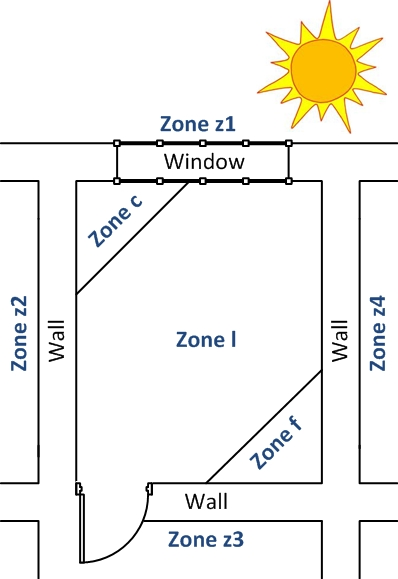
\includegraphics[width=2.5in,keepaspectratio]{./figs/zone1.jpg}
\caption{Zone}
\label{fig:zone}
\end{figure}

\begin{figure}[t]
\centering
	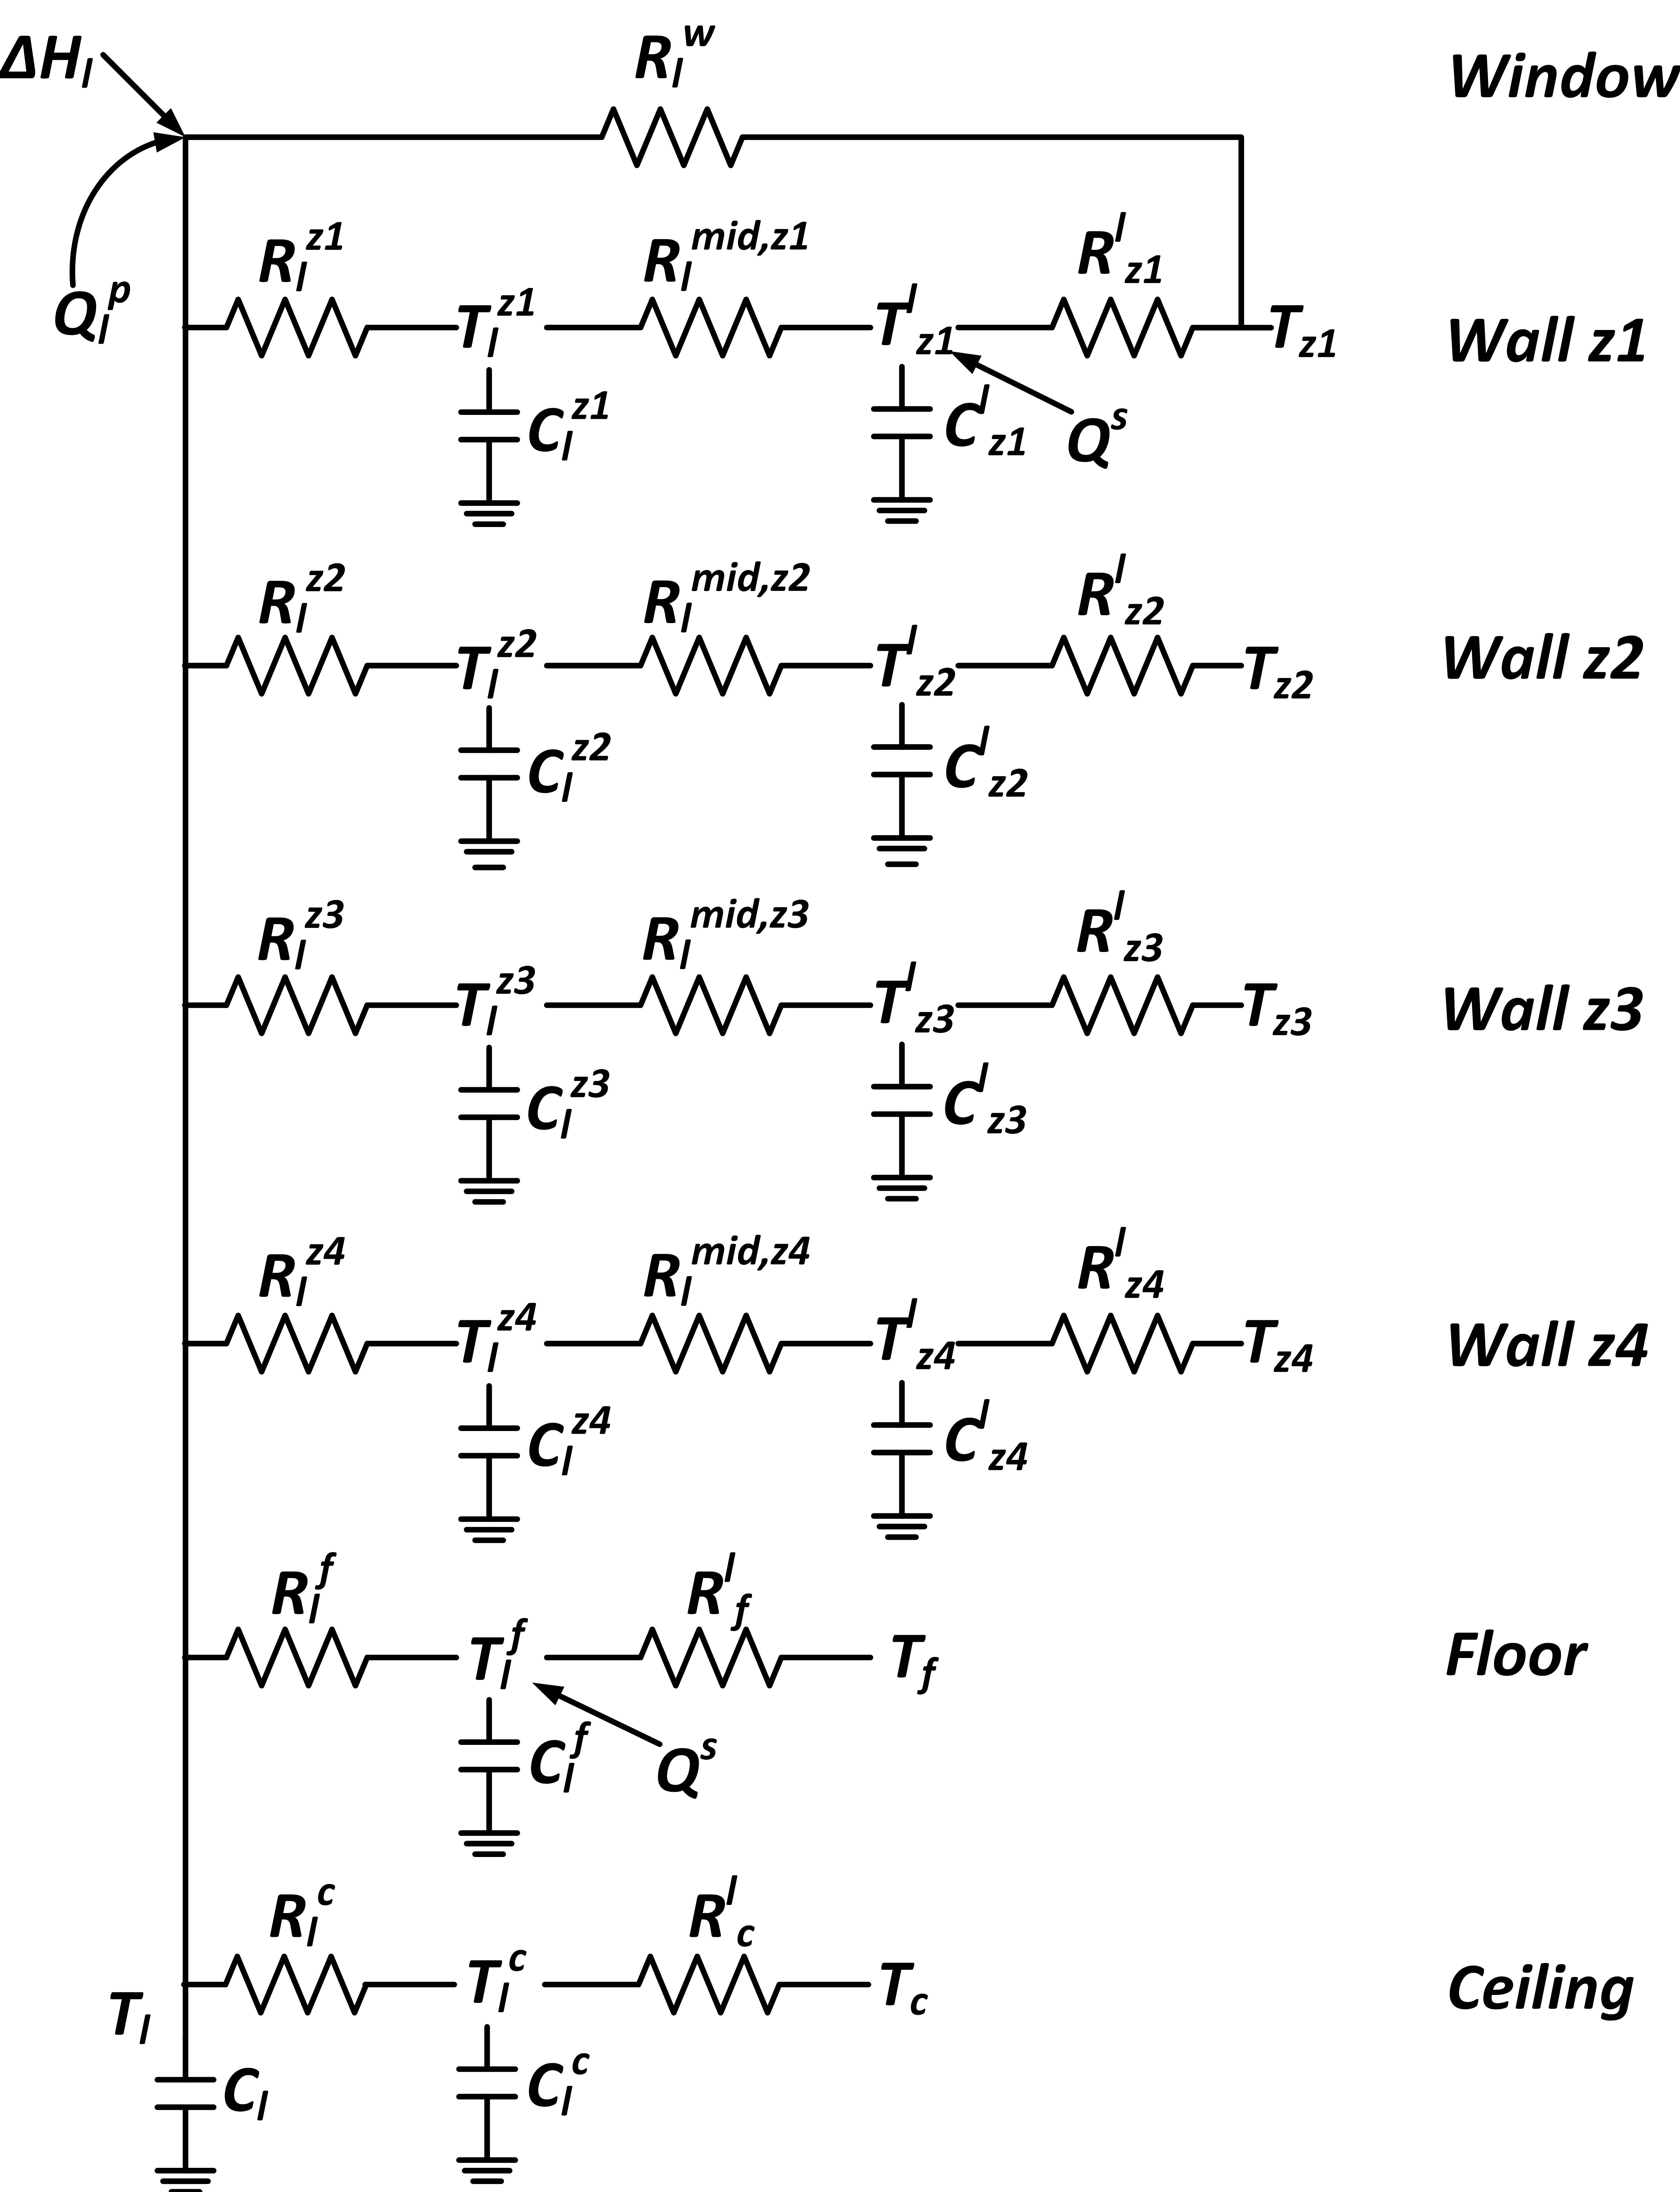
\includegraphics[width=4.0in,keepaspectratio]{./figs/3r2c.jpg}
\caption{Lumped-RC Network}
\label{fig:network}
\end{figure}

The principles behind the thermal model are represented in Figure \ref{fig:zone} and Figure \ref{fig:network}. Figure \ref{fig:zone} shows the zone structure that we adopt. Zone $l$ is separated by a wall and a window from zone $z1$ and by a wall from zones $z2$, $z3$, and $z4$, which could represent either indoor or outdoor zones. It is also separated by the ceiling and floor from zones $c$ and $f$ which are above and below zone $l$, respectively. Zone $l$ has a capacitance $\bm{C_l}$ that models the heat capacity of the air in the zone.  It also has a solar gain $Q^{s}_{l,k}$ and heat gain $Q^{p}_{l,k}$ at time step $k$. Moreover, the inner (resp. outer) wall separating $l$ from zone $z\in Z= \left\{z1,z2,z3,z4,f,c\right\}$ has a capacitance $\bm{C^z_l}$ (resp. $\bm{C^l_z}$), resistance $\bm{R^z_l}$ (resp. $\bm{R^l_z}$), and temperature $T^z_{l,k}$ (resp. $T^l_{z,k}$) at time step $k$. The window has a resistance $\bm{R^w_l}$. Finally, the internal node between the inner and outer walls separating $l$ from $z\in\{z1,z2,z3,z4\}$ has a constant resistance $\bm{R^{mid,z}_l}$. Capacitances, resistances, solar gain, and (in this section) occupant heat gain are inputs to the model whilst temperatures are auxiliary variables. The interaction between zones is modeled using a lumped RC-network. Specifically, we use 3R2C for walls separating two zones, 2R1C for the ceiling and floor and 1R for windows. The lumped network for Figure~\ref{fig:zone} is given in Figure~\ref{fig:network}.

The lumped network translates into a set of coupled difference equations which can be summarised as follows. The first difference equation defines the temperature $T_{l,k}$ in zone $l$ at time step $k$ as a function of the location, inner walls, ceiling, floor and outdoor temperatures at the previous time step, of the heat gain $Q^p_{l,k-1}$ at the previous time step and of the enthalpy $\Delta H_{l,k-1}$ of the location due to the supply air: 

\begin{equation}\label{eq:roomtemperature}
\begin{split}
{T}_{l,k} = 
\left[ 1 - \frac{\bm{\Delta t}}{\bm{C_l}} (\sum_{z\in Z} \frac{1}{\bm{R^z_l}} + \frac{1}{\bm{R^w_l}})  \right] T_{l,k-1} + 
\sum_{z\in Z} \frac{\bm{\Delta t}}{{\bm{C_l}}{\bm{R^z_l}}} T^{z}_{l,k-1} + 
\frac{\bm{\Delta t}}{{\bm{C_l}}\bm{{R^{w}_l}}} \bm{T^{OA}_{k-1}} 
& + \frac{\bm{\Delta t}}{\bm{C_l}} \Delta H_{l,k-1} \\
& + \frac{\bm{\Delta t}}{\bm{C_l}} Q^{p}_{l,k-1} 
\end{split}
\end{equation}

%
%\begin{equation} \label{eq:roomtemperature}
%\begin{split}
%\frac{{C}_l}{\Delta t}({T}_{l,k} -T_{l,k-1}) = 
%- \left[
%\sum_{z\in Z} \frac{1}{\bm{R^z_l}} +
%\frac{1}{\bm{R^w_l}}
%\right] T_{l,k-1} \\
%+ \sum_{z\in Z}\frac{T^{z}_{l,k-1}}{\bm{R^z_l}} +
%\frac{\bm{T^{OA}_{k-1}}}{\bm{R^w_l}}
%+ Q^{p}_{l,k-1} + \Delta H_{l,k-1}
%\end{split}
%\end{equation}

\noindent The heat gain $Q^p_{l,k}$ is simply the heat gain $q^p$ generated per person (75W), times the number of occupants $pp_{l,k}$:
\begin{equation} \label{eq:heatgain}
Q^{p}_{l,k} = \bm{q^{p}} \times pp_{l,k}
\end{equation}

\noindent Ignoring humidity, the enthalpy is defined as follows:
\begin{equation} \label{eq:enthalpy}
\Delta H_{l,k} = \bm{C^{pa}} a^{SA}_{l,k} (T^{SA}_{l,k} - T_{l,k})
\end{equation}
%\vspace*{-1px}
The remaining difference equations define the temperatures $T^z_{l,k}$ and $T^l_{z,k}$ of the inner and outer walls at time step $k$ as a
function of each other and of the location temperature $T_{l,k-1}$ at the previous time step. 

Taking $z=z1$ in the example of Figure~\ref{fig:zone}:

\begin{equation}\label{eq:temp:outer}
T^{z}_{l,k} = 
\left[ 1 - \frac{\bm{\Delta t}}{\bm{C_l^z}} (\frac{1}{\bm{R^z_l}} +  \frac{1}{\bm{R^{mid,z}_l}} )  \right] T^{z}_{l,k-1} + 
\frac{\bm{\Delta t}}{{\bm{C_l^z}}{\bm{R^z_l}}} T_{l,k-1} + 
\frac{\bm{\Delta t}}{{\bm{C_l^z}}{\bm{R^{mid,z}_l}}} T^{l}_{z,k-1} 
\end{equation}

\begin{equation}\label{eq:temp:inner}
T^{l}_{z,k} = 
\left[ 1 - \frac{\bm{\Delta t}}{\bm{C_z^l}} (\frac{1}{{R}^{l}_z} +  \frac{1}{\bm{R^{mid,z}_l}} )  \right] T^{l}_{z,k-1} + 
\frac{\bm{\Delta t}}{{\bm{C_z^l}}{\bm{R^l_z}}} \bm{T^{OA}_{k-1}} + 
\frac{\bm{\Delta t}}{{\bm{C_z^l}}{\bm{R^{mid,z}_l}}} T^{z}_{l,k-1} +
\frac{\bm{\Delta t}}{{\bm{C_z^l}}} \bm{Q^{s}_{l,k-1}}
\end{equation}

\noindent Observe that the definition of the inner wall temperature $T^{z}_{l,k}$ is symmetrical to that of the outer wall temperature $T^{l}_{z,k}$ except for the absence of solar gain $\bm{Q^s_{k-1}}$, and the replacement of the outdoor temperature $\bm{T^{OA}_{k-1}}$ with the room temperature $T^{z}_{l,k-1}$ of the neighbouring zone $z$.

%Note that if location $l$ has a wall separating it from room $z$, then $\bm{T^{OA}_{k-1}}$ is replaced by $T^{z}_{l,k-1}$
%Note that if location $l$ has a wall that separate between two rooms instead of the outdoor environment, $\frac{\Delta t}{{\bm{C_z^l}}{\bm{R^l_z}}} \bm{T^{OA}_{k-1}}$ is replaced with $\frac{\Delta t}{{\bm{C_z^l}}{\bm{R^l_z}}} T_{nl, k-1}$ where $nl$ is the neighbouring zone $l$. The equations for the other walls are similar, so we omit them here.

The temperatures of the floor and the ceiling at time step $k$ is calculated as a function of the location temperature $T_{l,k-1}$, the outdoor temperature $\bm{T^{OA}}$ and the solar gain $Q^{s}$ at the previous time step. 
\begin{equation}\label{eq:tlf}
T^{f}_{l,k} = 
\left[ 1 - \frac{\bm{\Delta t}}{\bm{C_l^f}} (\frac{1}{\bm{R^f_l}} +  \frac{1}{\bm{R^l_f}} )  \right] T^{f}_{l,k-1} + 
\frac{\bm{\Delta t}}{{\bm{C_l^f}}{\bm{R^f_l}}} T_{l,k-1} + 
\frac{\bm{\Delta t}}{{\bm{C_l^f}}{\bm{R^l_f}}} \bm{T^{OA}_{k-1}} +
\frac{\bm{\Delta t}}{{\bm{C_l^f}}} \bm{Q^{s}_{l,k-1}}
\end{equation}

\begin{equation}\label{eq:tlc}
T^{c}_{l,k} = 
\left[ 1 - \frac{\bm{\Delta t}}{\bm{C_l^c}} (\frac{1}{\bm{R^c_l}} +  \frac{1}{\bm{R^l_c}} )  \right] T^{c}_{l,k-1} + 
\frac{\bm{\Delta t}}{{\bm{C_l^c}}{\bm{R^c_l}}} T_{l,k-1} + 
\frac{\bm{\Delta t}}{{\bm{C_l^c}}{\bm{R^l_c}}} \bm{T^{OA}_{k-1}} 
\end{equation}

%\begin{equation} \label{eq:temp:outer}
	%\begin{split}
	%\frac{{C}^{l}_{z1}}{\Delta t} (T^{l}_{z1,k} \!-\! T^{l}_{z1,k-1}) =
		%- \left[
		%\frac{1}{{R}^{l}_{z1}} +
		%\frac{1}{{R}^{mid,z1}_l}
				%\right] T^{l}_{z1,k-1} 
		%+\frac{T_{z1,k-1}}{{R}^{l}_{z1}} +
                  %\frac{T^{z1}_{l,k-1}}{{R}^{mid,z1}_l} +
		%Q^s_{k-1}
	%\end{split}
%\end{equation}


\subsection{MILP Relaxation}
\label{subsec:relaxation}
Observe that the model as presented so far is a mixed-integer {\em non-linear} (MINLP) model. This is because of the bilinear terms $a_{l,k}^{SA}T_{l,k}^{SA}$ and $a_{l,k}^{SA}T_{l,k}$ in Equations~\eqref{eq:p_heat} and~\eqref{eq:enthalpy}. From a computational standpoint, it is better to relax these equations so as to obtain a MILP for which effective solvers exist that are guaranteed to return a lower bound on the globally optimal MINLP objective.  To obtain a suitable MILP, we use the linear programming relaxation of bilinear terms introduced by \cite{mccormick1976computability}. This relaxation introduces a new variable $v$ for the bilinear term $xy$ together with four
inequalities that define its convex envelope using the bounds $[\underline{x},\overline{x}]$ and $[\underline{y},\overline{y}]$ on each of the two variables involved:

\[\begin{array}{l}
v \geq \underline{x}y + \underline{y}x - \underline{x}\underline{y}\\
v \geq \overline{x}y + \overline{y}x - \overline{x}\overline{y}\\
v \leq \underline{x}y + \overline{y}x - \underline{x}\overline{y}\\
v \leq \overline{x}y + \underline{y}x - \overline{x}\underline{y}
\end{array}
\]

Hence, our MILP model is obtained by replacing the bilinear terms $a_{l,k}^{SA}T_{l,k}^{SA}$ with new variable $aT_{l,k}^{SA,SA}$ and $a_{l,k}^{SA}T_{l,k}$ with new variable $aT_{l,k}^{SA,z}$ in Equations~\eqref{eq:p_heat} and~\eqref{eq:enthalpy} and adding the corresponding convex envelope definitions. 

The new variable $aT_{l,k}^{SA,SA}$ is constrained by:
\begin{equation}
aT_{l,k}^{SA,SA} \geq \bm{\underline{a}^{SA}_{l,k}} T_{l,k}^{SA} + \bm{\underline{T}^{SA}_{l,k}} a_{l,k}^{SA} - \bm{\underline{a}^{SA}_{l,k}} \bm{\underline{T}^{SA}_{l,k}}\hspace{10pt} \forall l \in L, k \in K 
\end{equation}
\begin{equation}
aT_{l,k}^{SA,SA} \geq \bm{\overline{a}^{SA}_{l,k}} T_{l,k}^{SA} + \bm{\overline{T}^{SA}_{l,k}} a_{l,k}^{SA} - \bm{\overline{a}^{SA}_{l,k}} \bm{\overline{T}^{SA}_{l,k}}\hspace{10pt} \forall l \in L, k \in K 
\end{equation}
\begin{equation}
aT_{l,k}^{SA,SA} \leq  \bm{\underline{a}^{SA}_{l,k}} T_{l,k}^{SA} + \bm{\overline{T}^{SA}_{l,k}} a_{l,k}^{SA} - \bm{\underline{a}^{SA}_{l,k}} \bm{\overline{T}^{SA}_{l,k}}\hspace{10pt} \forall l \in L, k \in K 
\end{equation}
\begin{equation}
aT_{l,k}^{SA,SA} \leq  \bm{\overline{a}^{SA}_{l,k}} T_{l,k}^{SA} + \bm{\underline{T}^{SA}_{l,k}} a_{l,k}^{SA} - \bm{\overline{a}^{SA}_{l,k}} \bm{\underline{T}^{SA}_{l,k}}\hspace{10pt} \forall l \in L, k \in K 
\end{equation}

The new variable $aT_{l,k}^{SA,z}$ is constrained by:
\begin{equation} \label{eq:aSAT1} 
aT_{l,k}^{SA,z} \geq \bm{\underline{a}^{SA}_{l,k}} T_{l,k} + \bm{\underline{T}_{l,k}} a_{l,k}^{SA} - \bm{\underline{a}^{SA}_{l,k}} \bm{\underline{T}_{l,k}}  \hspace{10pt} \forall l \in L, k \in K 
\end{equation}
\begin{equation} \label{eq:aSAT2} 
aT_{l,k}^{SA,z} \geq \bm{\overline{a}^{SA}_{l,k}} T_{l,k} + \bm{\overline{T}_{l,k}} a_{l,k}^{SA} - \bm{\overline{a}^{SA}_{l,k}} \bm{\overline{T}_{l,k}} \hspace{10pt} \forall l \in L, k \in K 
\end{equation}
\begin{equation} \label{eq:aSAT3} 
aT_{l,k}^{SA,z} \leq  \bm{\underline{a}^{SA}_{l,k}} T_{l,k} + \bm{\overline{T}_{l,k}} a_{l,k}^{SA} - \bm{\underline{a}^{SA}_{l,k}} \bm{\overline{T}_{l,k}} \hspace{10pt} \forall l \in L, k \in K 
\end{equation}
\begin{equation} \label{eq:aSAT4} 
aT_{l,k}^{SA,z} \leq  \bm{\overline{a}^{SA}_{l,k}} T_{l,k} + \bm{\underline{T}_{l,k}} a_{l,k}^{SA} - \bm{\overline{a}^{SA}_{l,k}} \bm{\underline{T}_{l,k}}  \hspace{10pt} \forall l \in L, k \in K 
\end{equation}

The relevant bounds are:

\begin{itemize}
\item $a_{l,k}^{SA} \in [\bm{\underline{a}^{SA}_{l,k}}, \bm{\overline{a}^{SA}_{l,k}}] = 
\left\{
\begin{array}{ll}
\![\bm{\underline{a}^{SA}},\bm{\overline{a}^{SA}}_l] & \mbox{for $k\in K^s$}\\
\![0,\bm{\overline{a}^{SA}}] & \mbox{for $k\in K\setminus K^s$}\\
\end{array}
\right.$

\item $T_{l,k}^{SA} \in [\bm{\underline{T}^{SA}_{l,k}}, \bm{\overline{T}^{SA}_{l,k}}] = 
\left\{
\begin{array}{ll}
\![\bm{T^{CA}},\bm{\overline{T}^{SA}}] & \mbox{for $k \in K^s$}\\
\![0,\bm{\overline{T}^{SA}}] & \mbox{for $k \in K \setminus K^s$}\\
\end{array}
\right.$

\item $T_{l,k}\in [\underline{T}_{l,k}, \overline{T}_{l,k}] = [\undersl{\bm T}^{\bm \emptyset} ,\oversl{\bm T}^{\bm \emptyset} ]$ for $k\in K$
\end{itemize}

This concludes the description of our MILP model for occupancy-based HVAC control. Given the occupancy $pp_{l,k}$ and $z_{l,k}$, and the
external temperature $\bm{T^{OA}_{k}}$, it controls the supply air flow rate $a^{SA}_{l,k}$ and temperature $T^{SA}_{l,k}$ and decides when a
location requires HVAC activation $w_{l,k}$ out of the standby mode, in such a way as to optimise the total energy consumption $\sum_{k\in
  K}e_k$. The strengths of this model are its integration of realism and computational efficiency, its adequacy as a component of occupancy
scheduling and other more complex models, and its optional ability to activate out of the standby mode when this improves consumption.

\vspace*{10ex}
\section{Occupancy Scheduling}
\label{sec:mip:scheduling}
%\vspace*{-1ex}
Until now, zone occupancy over time was a model input. We now present our joint HVAC control and meeting scheduling model, in which occupancy is a decision variable.

Let $M \subseteq \mathbb{N}$ be a set of meetings to be scheduled to take place at the locations in $L$ during the time horizon $K$. Each meeting $m\in M$ is characterised by the following inputs: its duration $d_{m} \in \mathbb{N}$ (number of time steps), the set of allowable time steps $K_m \subseteq K$ at which it can start, the set of allowable locations $L_m\subseteq M$ at which it can take place, and its set of attendees $P_m \subseteq A$, for some appropriate set of attendees $A$. In addition, let ${\cal C}(M) \subseteq 2^{M}$ be the set of meeting sets which have at least one attendee in common, that is ${\cal C}(M)=\{C\subseteq M \mid \forall m,m'\in C, P_m\cap P_{m'} \neq \emptyset \}$.  In practice, only pairs of incompatible meetings are needed. Note that the sets $K_m$ and $L_m$ can be used to encode a variety of situations, such as room capacity requirements and availability of special equipment such as video conferencing, as well as time deadlines for the meeting occurrence and attendee availability constraints.

The main scheduling variable is the boolean decision variable $x_{m,l,k}$ which is true if meeting $m\in M$ is scheduled to take place at location $l\in L_m$ starting at time step $k\in K_m$. The scheduling part of the model interacts with the HVAC control part via the auxiliary variables $z_{l,k}$, which, as before, is true if location $l$ is occupied at time step $k$, and $pp_{l,k} \in \mathbb{N}$, which, as before, represents the number of occupants at location $l$ at time step $k$. These terms are used in Equations~\eqref{eq:temp_cstr} and~\eqref{eq:heatgain}, respectively, but are now variables rather than inputs.

The set of MILP scheduling constraints are the following. The first constraints ensure that all meetings are scheduled to occur exactly once within the range of allowable locations and start times: 
\begin{equation} \label{eq:ms_every} 
\mathop{\sum \limits_{l\in L_m, k \in K_m}} x_{m,l,k}=1 \hspace{10pt} \forall m \in M 
\end{equation}

\noindent The second constraints ensure that if a location is occupied by a meeting then it is exclusively occupied by this meeting during
its entire duration: 
\begin{equation} \label{eq:ms_totalalloc} 
\mathop{\sum \limits_{\substack{m \in M, k' \in K_m\\ {\scriptsize \mbox{~such that~}}\\ l\in L_m {\scriptsize \mbox{~and~}} k-d_m+1 \leq k' \leq k}}} x_{m,l,k'} \leq z_{l,k} \hspace{10pt} \forall l \in L, k \in K
\end{equation}
						
\noindent As a result, no two meetings can occupy the same location at the same time step. Observe that Constraints \eqref{eq:ms_totalalloc} also determine the occupancy variable $z_{l,k}$ used in the occupancy-based HVAC control part of the joint model.

The following constraints establish the number of occupants $pp_{l,k}$ of each location $l$ at each time step $k$:
\begin{equation} \label{eq:ms_totalnum} 
\mathop{\sum \limits_{\substack{m
        \in M, k' \in K_m\\ {\scriptsize \mbox{~such that~}}\\ l\in
        L_m {\scriptsize \mbox{~and~}} k-d_m+1 \leq k' \leq
        k}}} x_{m,l,k'}\times \left| P_m\right| =
  {pp}_{l,k} \hspace{8pt} \forall l \in L, k \in K 
\end{equation}

\noindent This is used in Equations~\eqref{eq:heatgain} to establish the internal heat gain arising from occupancy.

Finally, the last constraints ensure that meetings with an intersecting attendee set cannot overlap in time:
\begin{equation} \label{eq:ms_meeting}
\mathop{\sum \limits_{\substack{m \in \nu, l \in L_m, k' \in K_m\\ 
{\scriptsize \mbox{~such that~}}\\
k-d_m+1 \leq k' \leq k}}}  x_{m,l,k'} \leq 1 \hspace{10pt} \forall k \in K, \nu \in {\cal C}(M)
\end{equation}

Our joint HVAC control and occupancy scheduling model is simply obtained by adding Equations~\eqref{eq:ms_every}-\eqref{eq:ms_meeting} to the HVAC control model given by Equations~\eqref{eq:objective}-\eqref{eq:aSAT4}. Equations~\eqref{eq:p_heat} and Equations~\eqref{eq:enthalpy} are linearised by replacing the bilinear term $a^{SA}_{l,k}T^{SA}_{l,k}$ with $aT^{SA,SA}_{l,k}$ and $a^{SA}_{l,k}T_{l,k}$ with $aT^{SA,z}_{l,k}$.  The model optimises the total energy consumed not only over the HVAC decision variables $a^{SA}_{l,k}$, $T^{SA}_{l,k}$ and $w_{l,k}$ as before, but also over the scheduling decision variables $x_{m,l,k}$. A building occupancy-based HVAC controller need only use the schedules $x_{m,l,k}$ produced. A conventional controller may instead use the bounds on room temperature and supply air flow rate/temperature determined by Equations~\eqref{eq:temp_cstr}, \eqref{eq:hvac_active_TSA} and~\eqref{eq:hvac_standby_ASA} as setpoints. 

This concludes the description of our joint HVAC control and occupancy scheduling model. The next section experimentally investigates its
benefits in terms of energy reduction, in comparison with more na\"{\i}ve integrations of scheduling and HVAC control. 


\section{Experiments}
\label{sec:mip:experiments}

Our experiments aim at assessing the impact of room and time slot selections to HVAC consumption, explaining the usefulness of the standby mode and demonstrating that our HVAC-aware scheduling model leads to significant consumption reduction (50\% to 70\% in our experiments) when compared to occupancy-based HVAC control using arbitrary schedules or energy-aware schedules generated by heuristic methods. 

Simulations are carried out for five different building types with similar geometry but with different thermal resistance and capacitance. They are referred to as building type 1--5 in Table \ref{tab:rc_wall_win}. Each building corresponds to a row of 4 co-located zones (or interchangeably, rooms), where all zones have the same geometric area of $6\times 10\times 3 \mbox{ m}^3$ with a window surface area of $4\times 2    \mbox{ m}^2$. The two middle zones have two external walls (the wall separates the zone to the outside), with an area size of $6\times 3 \mbox{ m}^2$ each. The corner zones have an additional $3\times 10 \mbox{ m}^2$ of external wall. All the other walls of the zone are called internal walls. Two adjacent zones are separated with an internal wall. The thermal capacitance and thermal resistance for each wall at each building types are empirically designed based on construction materials obtained from \cite{gouda2000low}, \cite{gouda2002building}, \cite{goyal2013occupancy} and \cite{ashrae2013fund}. The outdoor temperature is taken from the month of January in Canberra, Australia, which is a summer month in the Southern hemisphere. The solar gain ranges from 50 to 350 W/m$^2$ during the day. Each room has a capacity of 30 people. The duration between successive time steps is $\bm{\Delta t} = 30$min, giving more than enough time for thermal effects to occur.  The MILP models are solved using Gurobi 5.6 \citep{gurobi}. All experiments were conducted on a cluster consisting of $2\times$ AMD 6-Core Opteron 4184, 2.8 GHz with 64 GB of memory.

\begin{table*}[t]
\centering
\begin{tabular}{p{0.2\linewidth} p{0.1\linewidth} p{0.1\linewidth}  p{0.1\linewidth} p{0.1\linewidth} p{0.1\linewidth}}
\hline\centering{Building Types} & \multicolumn{2}{c}{External Wall} & \multicolumn{2}{c}{Internal Wall} & {Window} \tabularnewline
       & \centering{(TR)} & \centering{(TC)} & \centering{(TR)} & \centering{(TC)} & \centering{(TR)} \tabularnewline
\hline \centering{1 (LRLC)} & \centering{3} & \centering{120} & \centering{1.5} & \centering{120} & \centering{0.5} \tabularnewline
\hline \centering{2 (MRMC)} & \centering{3} & \centering{140} & \centering{1.5} & \centering{140} & \centering{0.5} \tabularnewline
\hline \centering{3 (LRHC)} & \centering{3} & \centering{240} & \centering{1.5} & \centering{240} & \centering{0.5} \tabularnewline
\hline \centering{4 (HRLC)} & \centering{6} & \centering{120} & \centering{3} & \centering{120} & \centering{0.5} \tabularnewline
\hline \centering{5 (HRHC)} & \centering{6} & \centering{240} & \centering{3} & \centering{240} & \centering{0.5} \tabularnewline
\end{tabular}
	\caption{Total thermal resistance (TR) $\left( m^2 K\over W\right)$ and thermal capacitance (TC) $\left( KJ \over m^2K \right)$ of the walls and the window for five types of zones. The zones differ by a high (H), medium (M) and low (L) value for their thermal resistance (R) and capacitance (C). R and C of each wall can be derived by dividing TR and multiplying TC with area size respectively.}
	\label{tab:rc_wall_win}
\end{table*}


\subsection{Impacts of Room Selections and Time Allocations}

We start by studying the impact of room selections and time allocations for meetings on the HVAC consumption, through three simple case studies. We strive to answer two questions:
\begin{enumerate}
	\item Does room selection impact HVAC consumption?
	\item Does time allocation impact HVAC consumption?
	%\item Does room selection and time allocation impact HVAC control?
\end{enumerate}
\noindent Our goal is to provide evidence that room and time selections are crucial to reduce HVAC consumption.

\vspace{10px}
\emph{Case Study 1} \quad \textsl{How do building materials impact room temperature?}
\vspace{10px}

\begin{figure}
	\centering
		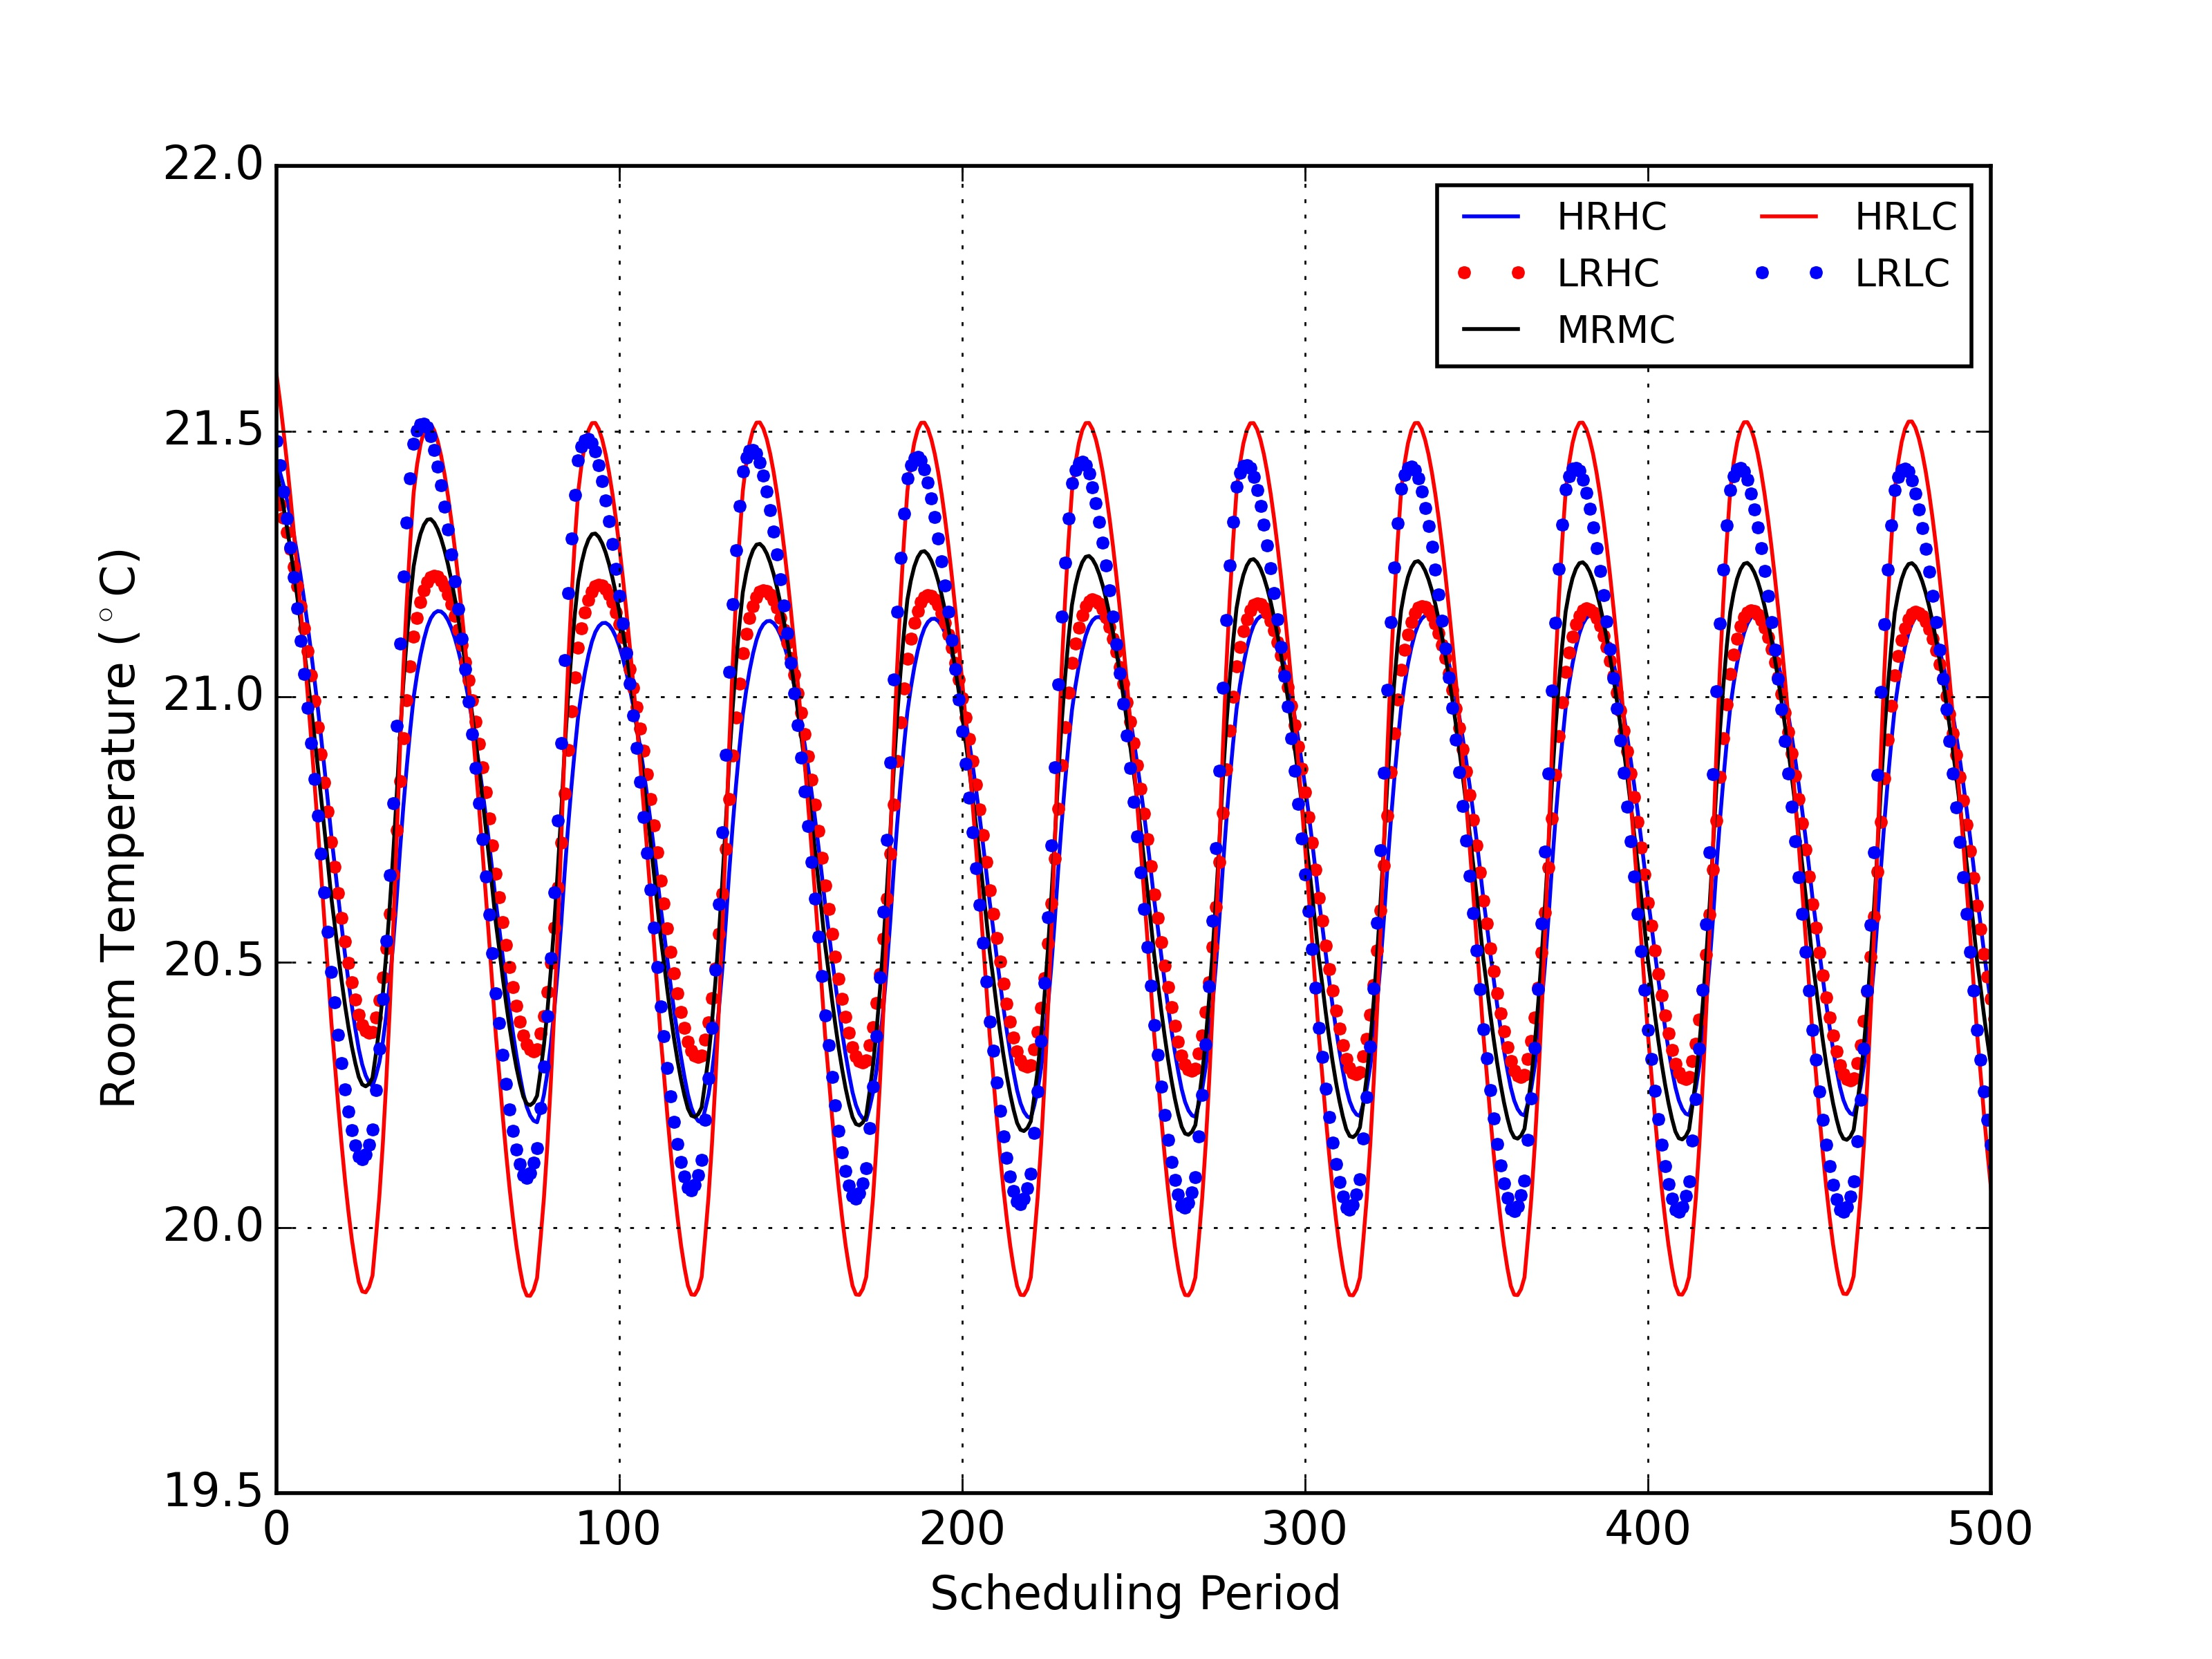
\includegraphics[width=0.74\linewidth,keepaspectratio]{./figs/mip_roomtemp.jpg}		
	\caption{Room temperature dynamics}
	\label{fig:mip_rt}
\end{figure}

Figure \ref{fig:mip_rt} illustrates the fluctuation of zone temperatures for 5 different building types, as defined in Table \ref{tab:rc_wall_win}. In this experiment, we assume that the HVAC is off and no meetings are scheduled. We simply calculate the zone temperature at each time step without optimizing any parameter. Thus, the zone temperatures are solely affected by the outdoor temperature and the solar gain. As the zones differ by a high (H), medium (M) and low (L) value for their thermal resistance (R) and capacitance (C), we observe that the temperatures at each zone fluctuate at a different scale. Some zones (eg. HRLC and LRLC) release and absorb heat at a faster rate, hence the zones' temperatures swing more drastically than other zones (eg. LRHC and HRHC). %At first, it may be seem that the latter zones are more energy efficient as the zones' temperature can be maintained at relatively smaller fluctuations, and be kept at a tighter comfort range. 
At first, it may seem that the latter zones are more energy efficient, as the zones' temperatures have relatively smaller fluctuations, and the room temperature can be kept within a tighter comfort range easily.
This is not necessarily true. The room temperatures are influenced by the diurnal temperature variation\footnote{Diurnal temperature variation is the variation between a high temperature and a low temperature that occurs during the same day.} of a location, and the energy consumption is impacted by the gap between outdoor temperature and the occupied comfort temperature range. Some building types require more energy for space heating or cooling at the beginning but they have better insulation to retain heat, whilst other building types have less insulation but are able to leverage the outdoor temperature to achieve comfort temperature for a short period of time. %require little energy  for space heating and cooling (passive house concept)
In the following, we look further into the HVAC consumption of each building types, with meetings being scheduled at different hours of a day.

\vspace{10px}
\emph{Case Study 2} \quad \textsl{How does meeting scheduling affect energy consumption at different rooms?}
\vspace{10px}

\begin{figure}
	\centering
		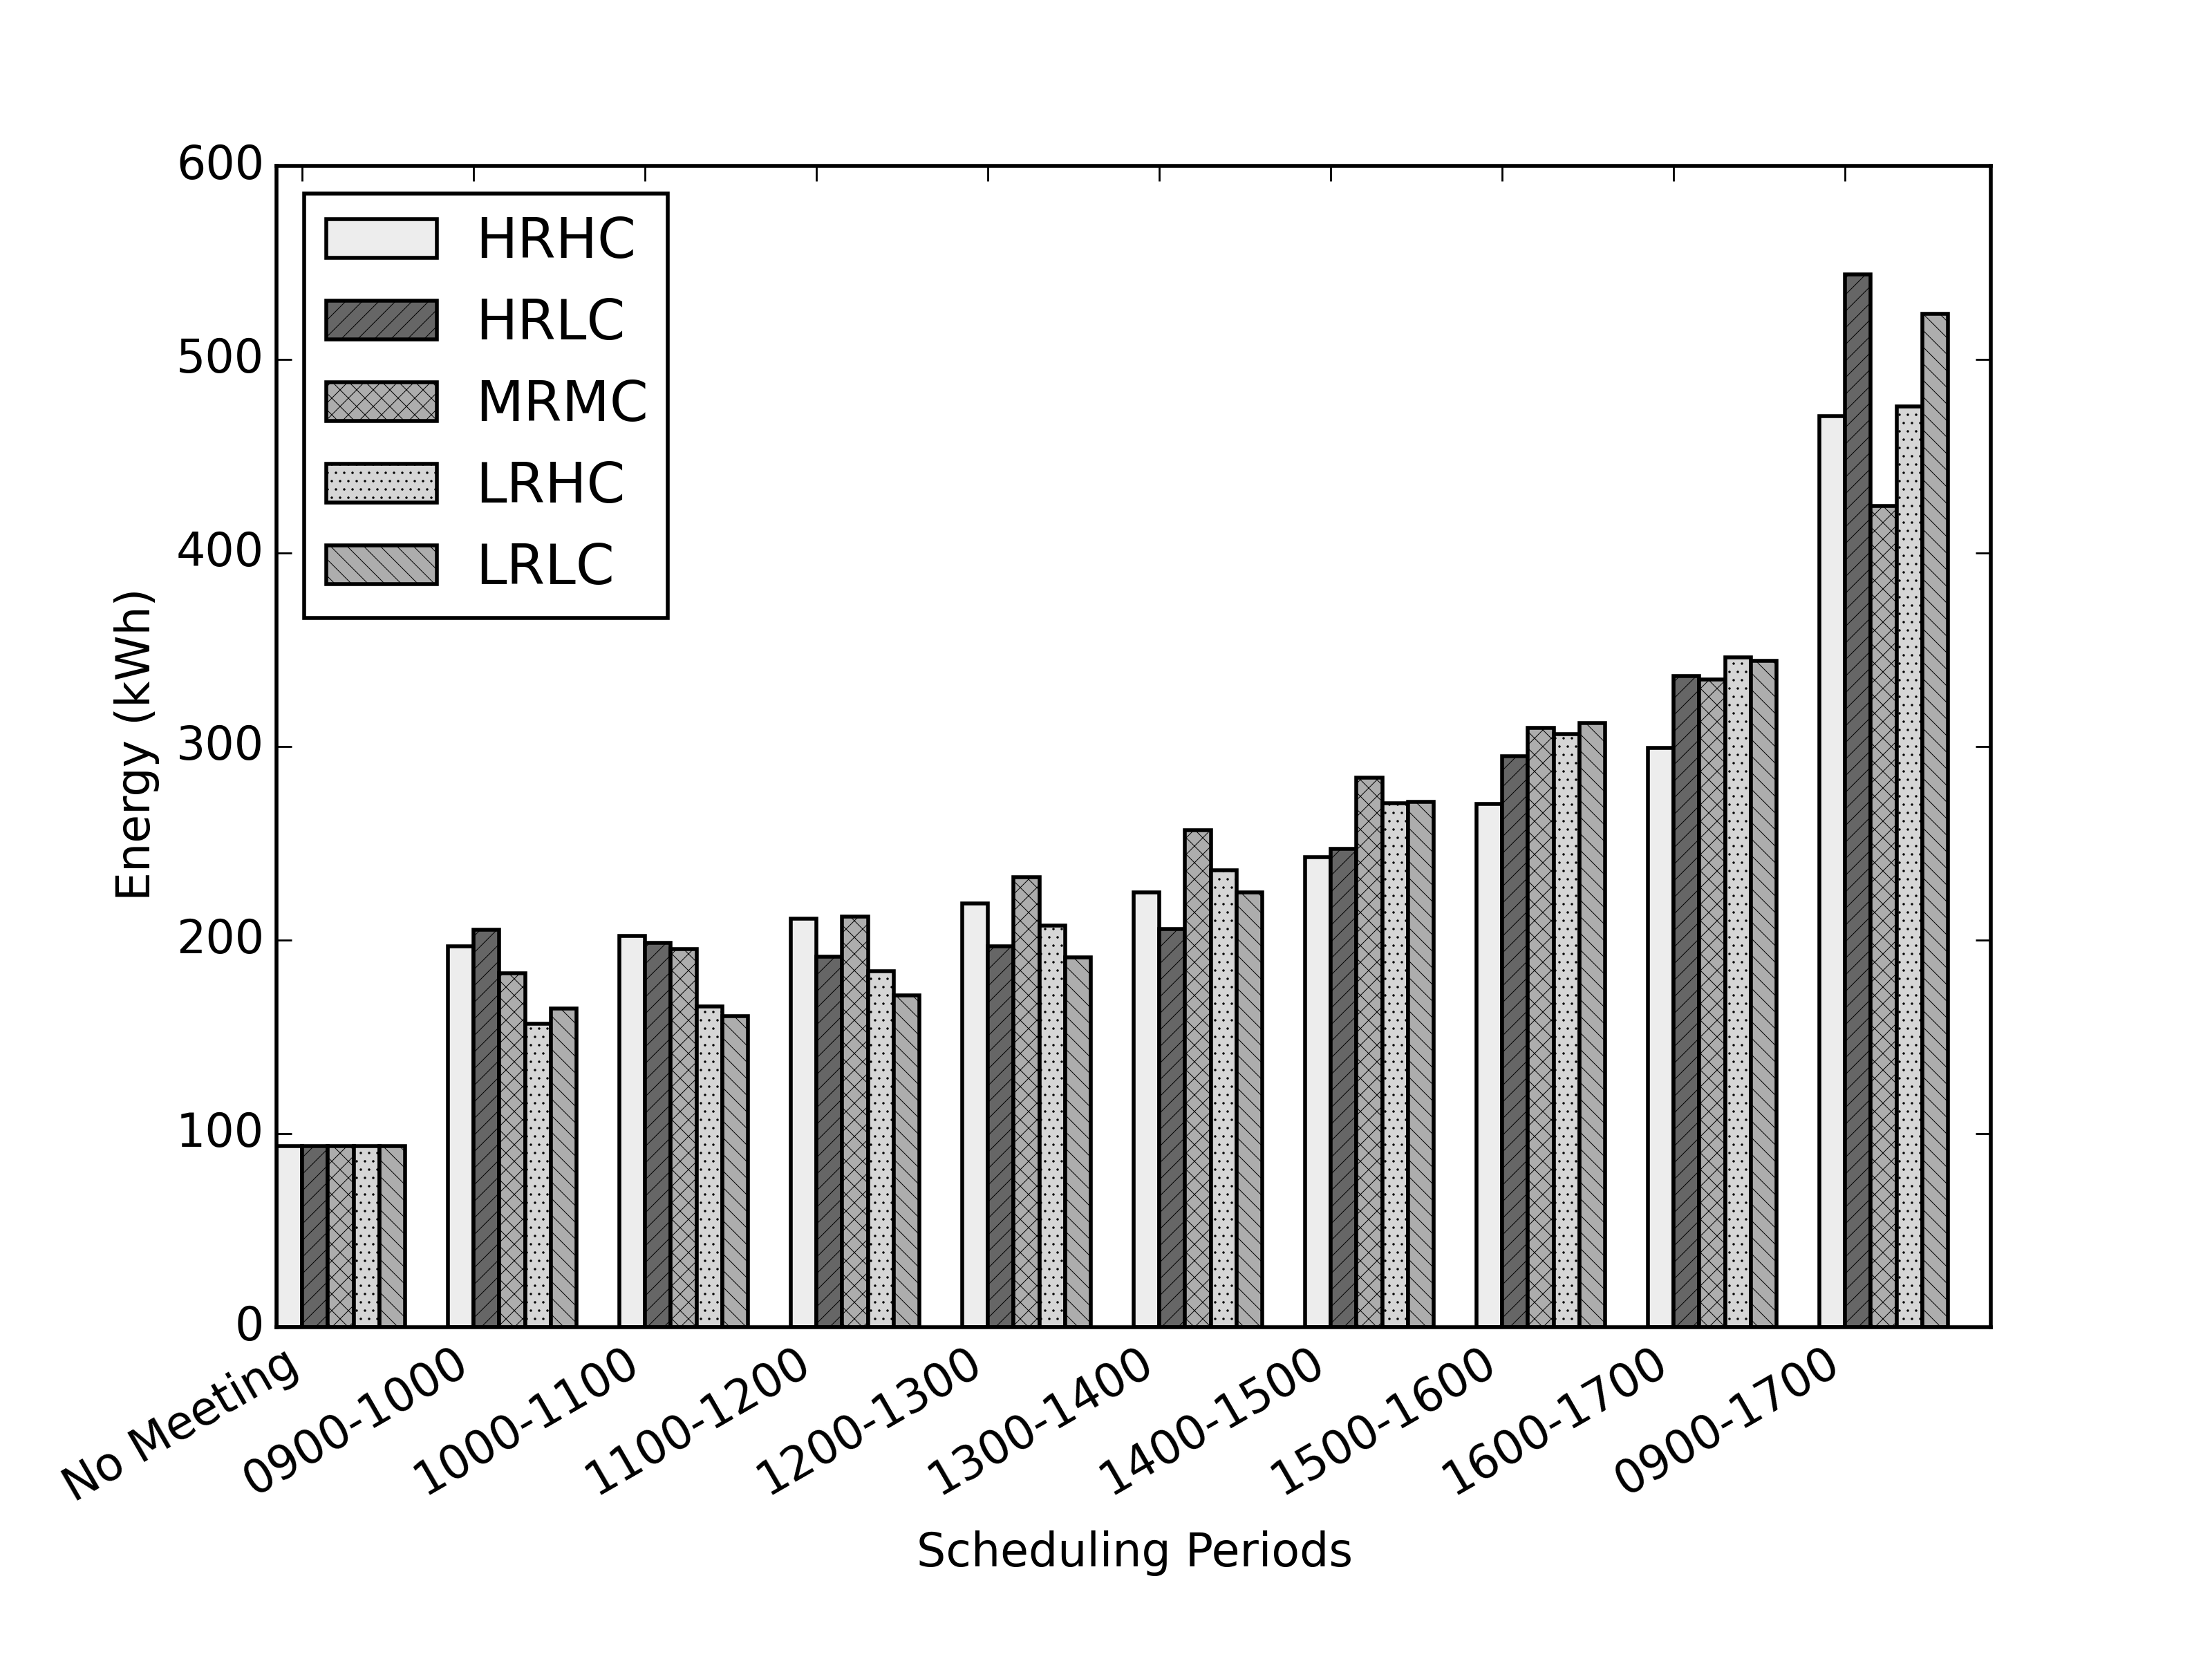
\includegraphics[width=0.74\linewidth,keepaspectratio]{./figs/mip_room_energy.png}		
	\caption{Energy consumption of different building types with meetings held at different time of the day}
	\label{fig:mip_re}
\end{figure}

Figure \ref{fig:mip_re} shows the energy consumption of 5 rooms located in different buildings, with meetings being held at different time of the day over 5 summer days. The meeting schedule is fixed, and the HVAC control is being optimized. The leftmost set of bars shows the energy consumption when no meeting is being held. The HVAC is turned on but running at a minimum load to maintain the basic ventilation standard required by \cite{ashrae2013thermal}. The rightmost set of bars shows the energy consumption when HVAC is turned on for an eight hour meeting held everyday. This setting can also be perceived as the conventional approach where HVAC is turned on throughout the day regardless of the occupancy of a zone. The rest of the graph shows the energy consumption for an hour meeting scheduled at the a given hour (e.g. 0900-1000) over 5 days. The HVAC is turned on to bring the zone temperature to 21$^\circ$C - 23$^\circ$C during occupied periods. We observe that the HVAC consumption increases when meetings are being scheduled in the evening compared to in the morning. This is due to the increase of cooling load required as the rooms get more heat gain from the sun during the afternoon and evening. However, the increase varies for different building types. The energy consumption patterns for each room type change with meetings being scheduled in the room at different hours of the day. Some consume less energy than other room types for a morning meeting, and vice versa for an evening meeting. Given various scheduling constraints, it is impossible to enumerate energy consumption patterns for all combinations of different schedules. Hence, automatic selection of room and time is crucial to identify optimal scheduling options and minimise HVAC expenses. 

\vspace{10px}
\emph{Case Study 3} \quad \textsl{Which room consumes the least amount of energy in a building?}
\vspace{10px}

\begin{figure}
	\centering
		\includegraphics[width=0.5\linewidth,keepaspectratio]{./figs/mip_roomsolar.jpg}		
	\caption{Energy consumption of 9 rooms with different facing and layout at LRHC building.}
	\label{fig:mip_rs}
\end{figure}

Next, we examine if room selection is crucial for rooms with similar thermal resistance and capacitance, and that are located in the same building. The meeting schedule is fixed, and the HVAC control is being optimized. Figure \ref{fig:mip_rs} shows the energy consumption of 9 rooms that are co-located in the same building, but with different facing and layout. With an 8-hours meeting scheduled in each room for a summer day, the results show that each room consumes a slightly different amount of energy. While a building consists of multiple rooms with similar build-up, each room has different layout and window size. They also acquire different amounts of solar gain over a day. These factors impact their HVAC consumption. Notice that the center room (C) is surrounded by four internal walls, hence it is the least impacted by the outdoor temperature and the solar gain. Its energy consumption is the highest as more HVAC intervention is required for space cooling. Meanwhile, four corner rooms (NE, SE, NW, SW) which have larger windows and larger area size of external walls consume relatively less energy compared to the two middle rooms (N,S). This result shows that selecting a room within the same building with different layout and exploiting external weather conditions can be effective to reduce energy consumption, while meeting the occupant thermal comfort requirement.

\subsection{Usefulness of Standby Mode}
\label{subsec:experiments:standby}

\begin{figure}
\begin{tabular}{c}
  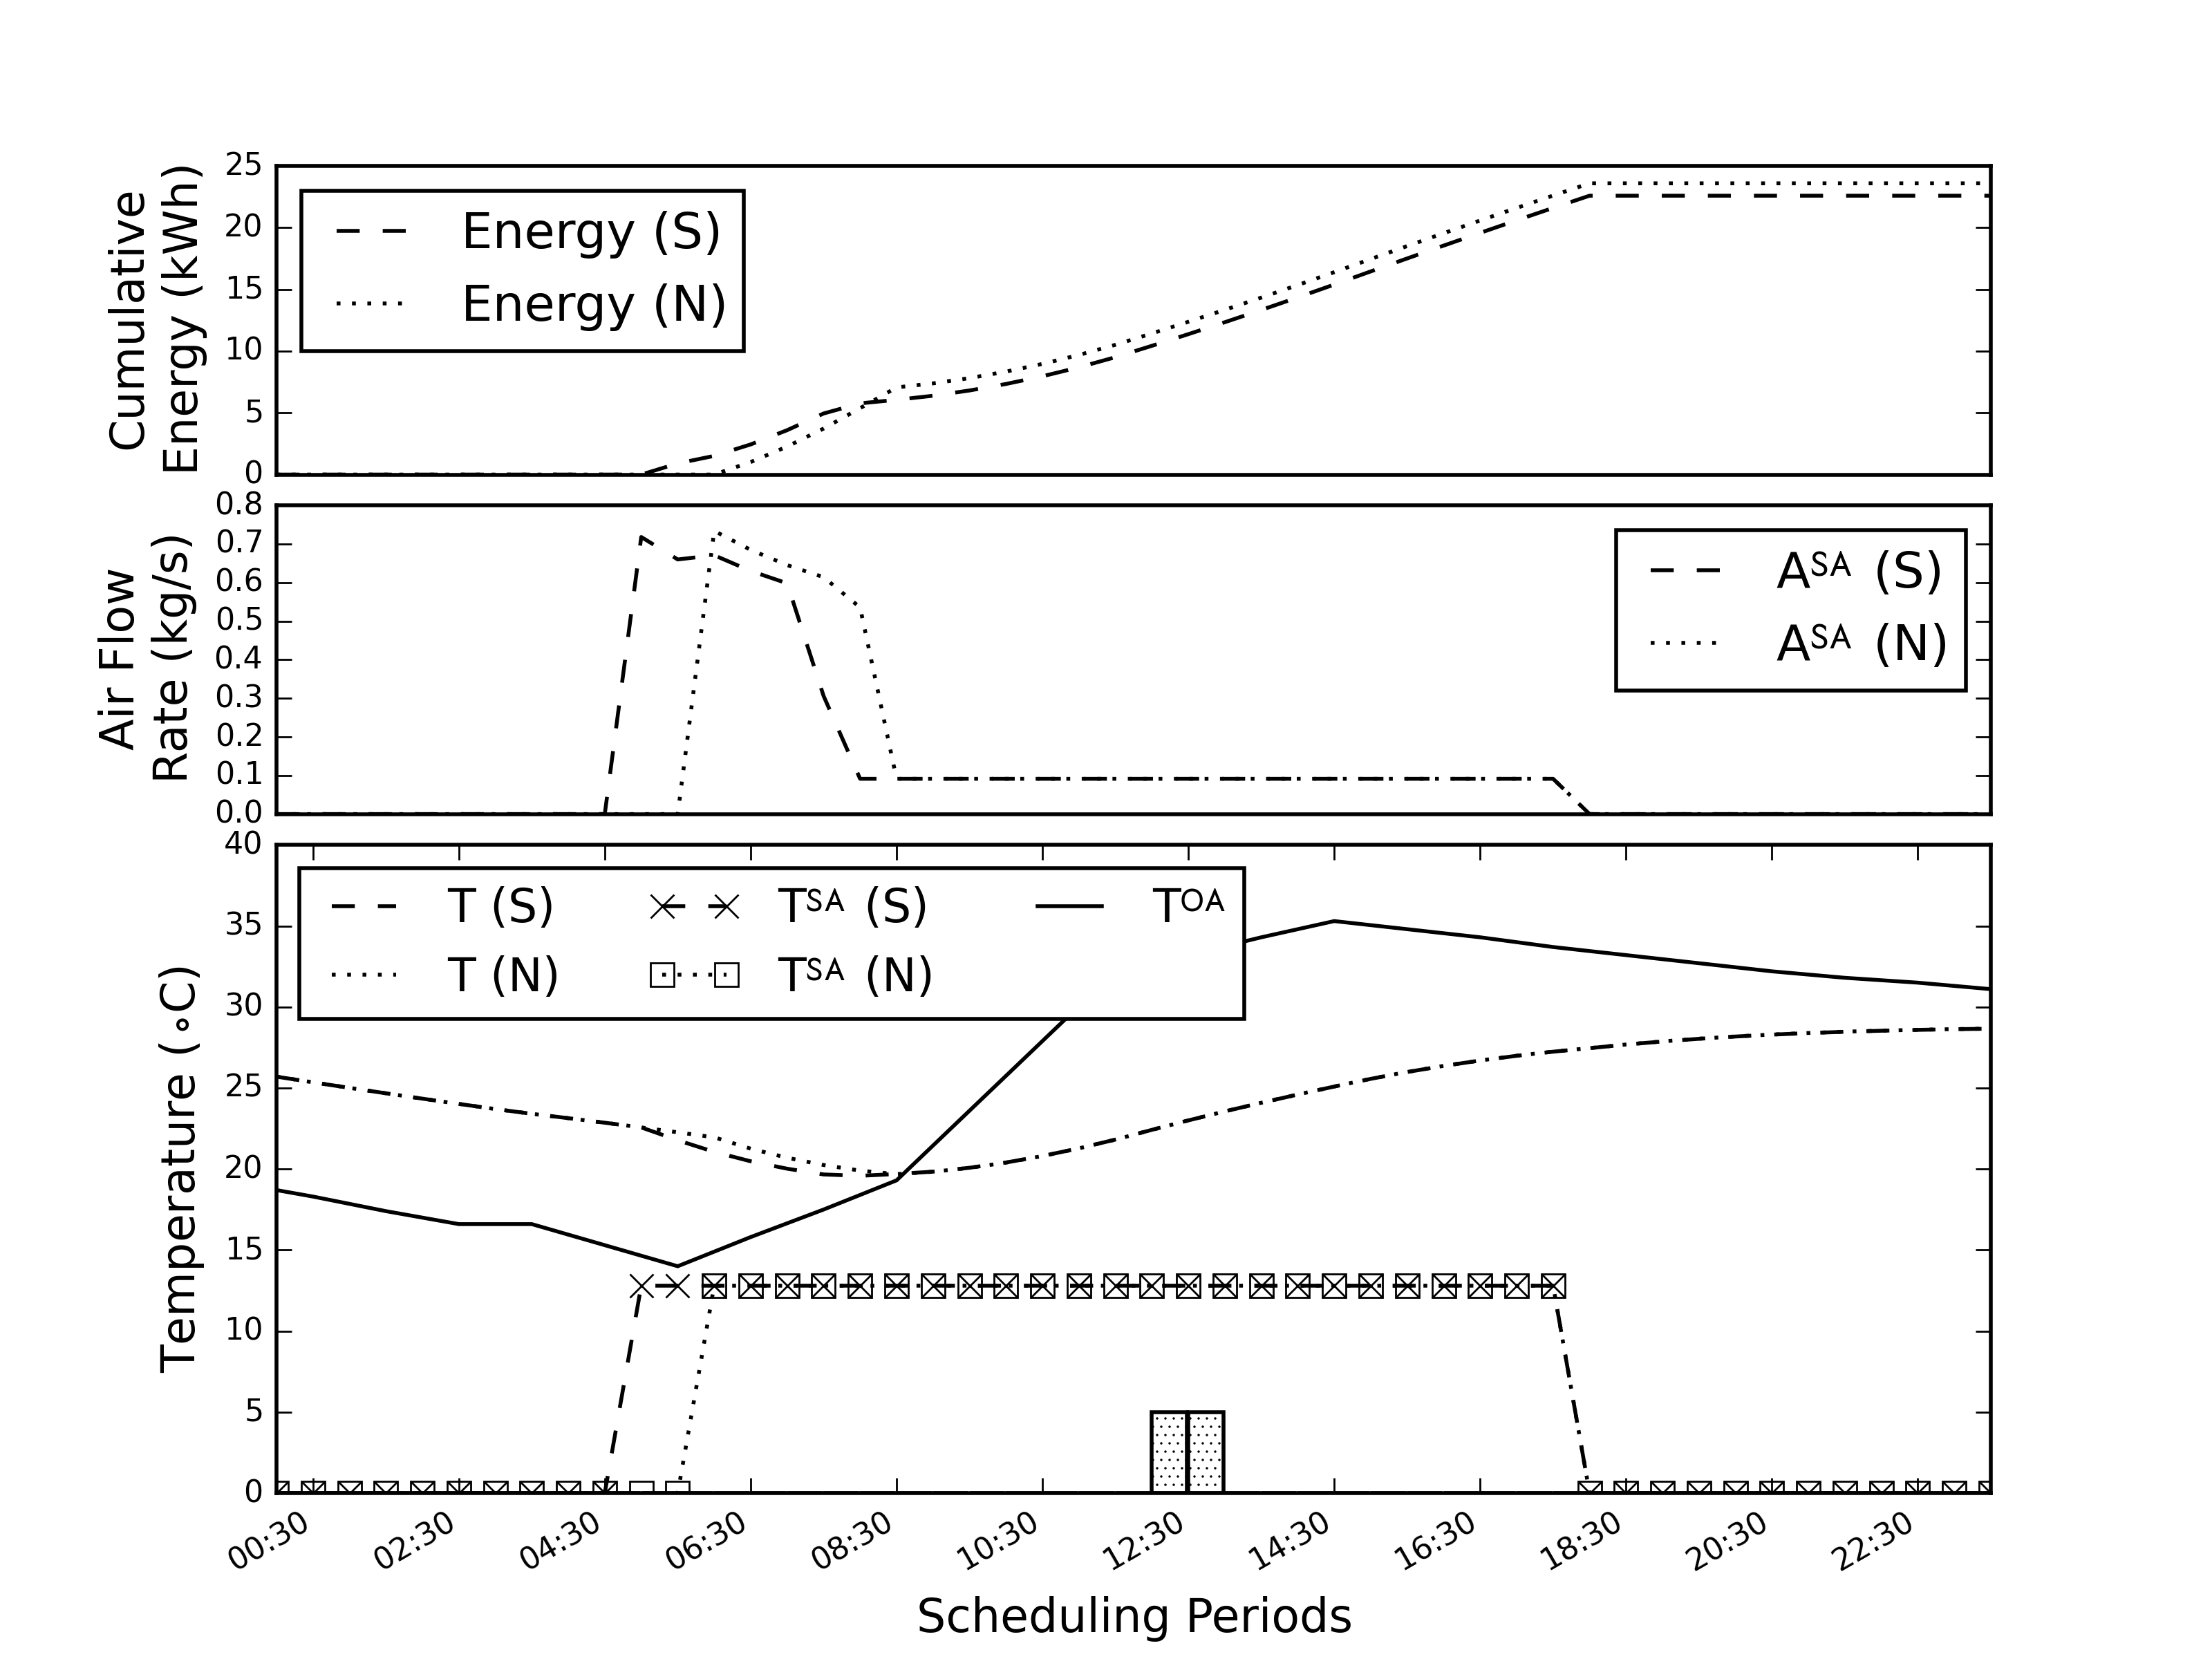
\includegraphics[width=0.9\linewidth]{figs/hrlc_opt_ws_ns_r0.png} \\
(a) HRLC \\[6pt]
  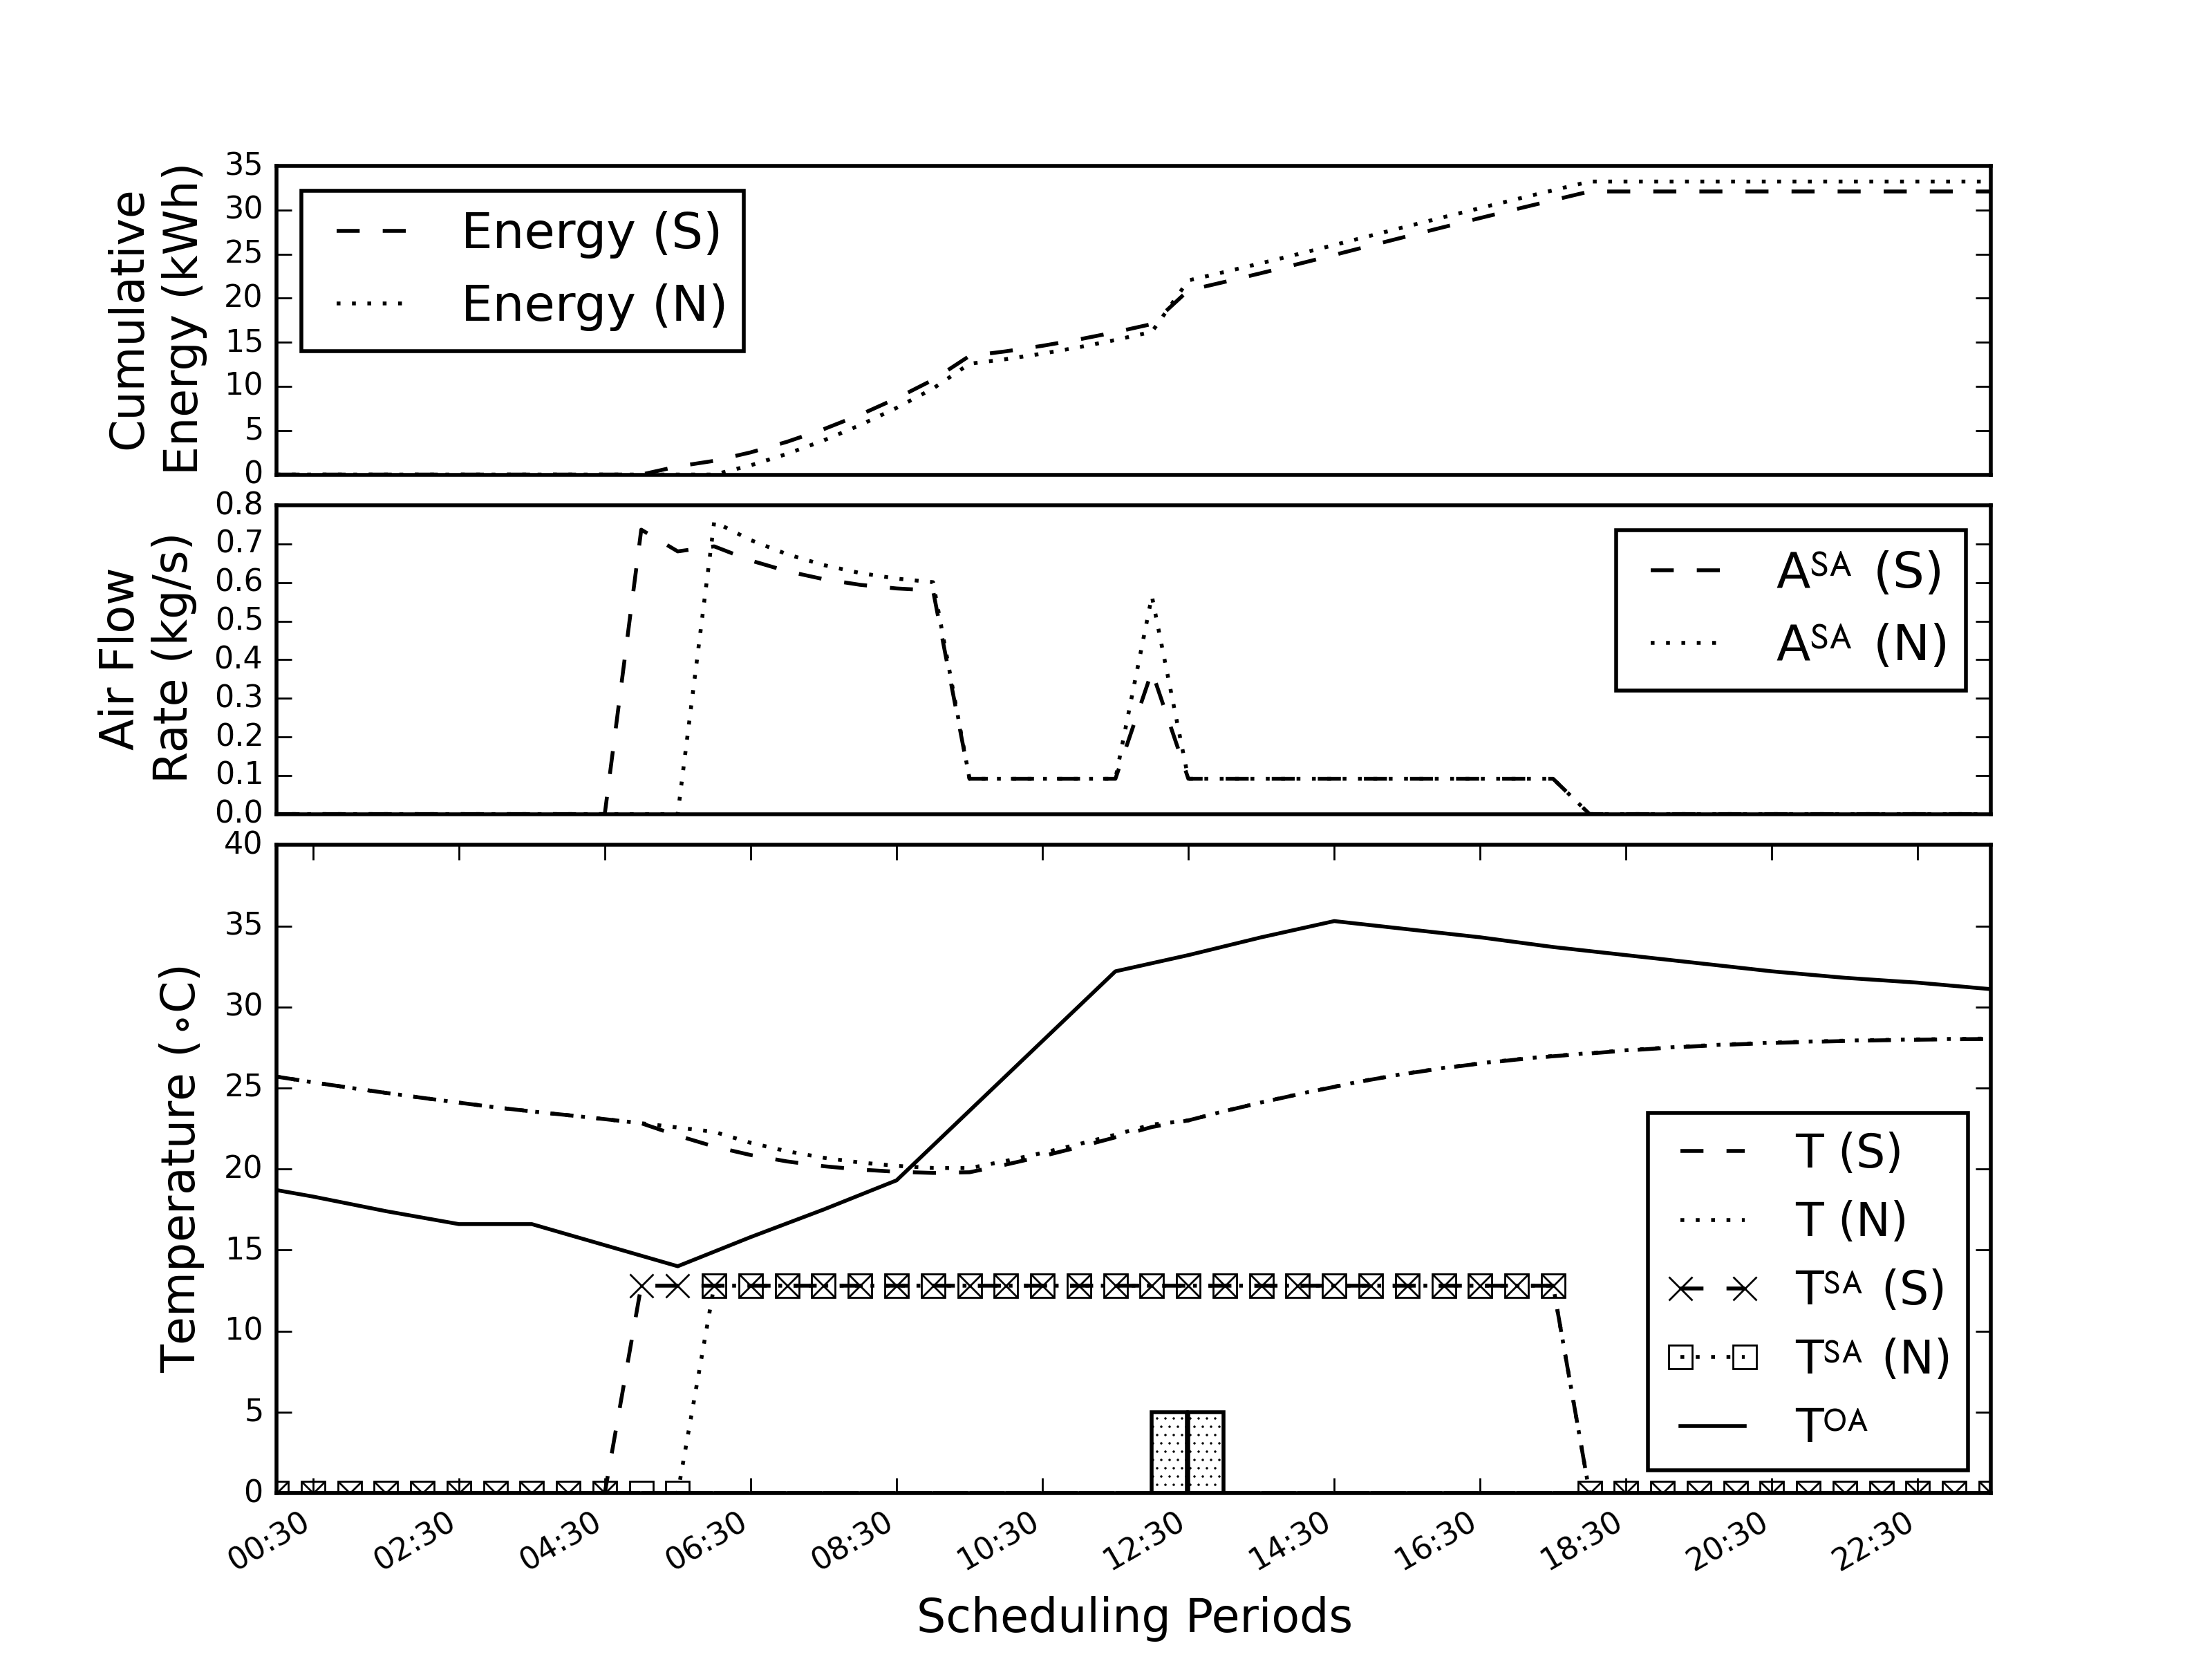
\includegraphics[width=0.9\linewidth]{figs/lrlc_opt_ws_ns_r0.png} \\
(b) LRLC \\[6pt]
\end{tabular}
\caption{HVAC control with (S) and without (N) standby mode. Our standby mode enables the HVAC to self activate outside business hours (eg. before 6 a.m.) for pre-cooling. This results in the reduction of energy consumption, compared to the HVAC control without standby mode.}
\label{fig:standby}
\end{figure}

Next we illustrate the usefulness of the standby mode. In conventional operations, HVACs are usually switched on a few hours prior to start of business (6am) and are turned off in the evening (6pm) and at night. Model predictive control strategies are capable of pre-cooling a zone, but only when the HVAC is switched on. Our standby mode enables the HVAC to self activate outside business hours to provide additional pre-cooling when this is beneficial. Because HVAC consumption is highly dependent on the temperature gap between the outdoor temperature and the conditioned air temperature, pre-cooling at night, when the outdoor air temperature is cooler, can reduce energy consumption. 
The following experiments show that such pre-cooling can be beneficial not only for early morning meetings, but also, more surprisingly, for afternoon meetings. 

Figure~\ref{fig:standby} compares the operations of the HVAC optimally controlled by the model in Section~\ref{sec:mip:control} with standby mode (S) and without standby mode (N). In this experiment, a single meeting is scheduled to occur between 12:00-13:00 in the HRLC zone and the LRLC zone of a given day. The occupied period is depicted as two vertical blocks (30 minutes each) in the third subgraph of Figure~\ref{fig:standby} (a) and (b). Observe that in the HRLC zone, when the HVAC is running with standby mode enabled, it activates as early as 05:00 and pushes between 0.72 and 0.3 kg/s of supply air at 12.8$^\circ$C to bring down the zone temperature to approximately 19$^\circ$C by 07:30. Between 04:30 and 06:00, the outdoor temperature lies between 14 and 15$^\circ$C, which is just about 1-2$^\circ$C higher than the 12.8$^\circ$C conditioned air temperature. In constrast, when the HVAC is running without the standby mode, the supply air is pushed into the room at a higher average rate between 0.73 and 0.53 kg/s right after the HVAC is turned on at 06:00, which, as the outdoor temperature is higher at that time (15-19$^\circ$C), requires a higher rate of energy consumption. During the day, the zone temperature increases slightly due to the daytime thermal gain, and at 12:00, the room temperature falls exactly within the comfort range of 21$^\circ$C - 23$^\circ$C. 

In the LRLC zone, a slightly different optimal control scheme is identified. With the standby mode enabled, the HVAC is activated at 05:00 and pushes between 0.73 and 0.58 kg/s of supply air at 12.8$^\circ$C until 09:00, where the room temperature reaches 20$^\circ$C. In contrast, with the standby mode disabled, the supply air is pushed into the room only from 06:00 to 09:00. Given that the outdoor temperature is rising, and the pre-cooling period is relatively short, it fails to bring down the room temperature further. At 12:00, when the meeting starts, the room is cooled down again. This time, the standby-mode enabled HVAC requires cooling about half the amount of supply air, which brings significant energy savings since the outside temperature is around 33$^\circ$C. 

Altogether, in both examples, the standby mode reduces consumption by 3.5-4.4\%. %(~1-2 kWh)
As shown above, a standby-mode-enabled HVAC can be effective in areas with high diurnal temperature variation.  In addition to decreasing energy consumption, it can provide pre-cooling at off-peak electricity cost. For organisations that are charged by electricity suppliers according to their peak consumption, another benefit of the standby mode is that it can help smooth the peak that is regularly observed at the start of the operating hours. We also notice that with standby mode, the scheduler is capable of generating more number of feasible solutions by reactivating the HVAC at off-peak hours in order to meet the occupied temperature bounds of an early morning meeting.


\subsection{Joint Model vs Simpler Models}
\label{subsec:experiments:integration}

Whilst the standby mode is beneficial, the much larger gains in our approach stem from the joint model: we now compare our joint model with simpler approaches representative of the existing literature on occupancy-based HVAC control and energy-aware meeting scheduling, and observe a significant energy consumption improvement.

Specifically, we consider a set of timetabling problems derived from the PATAT \cite{patat02} dataset 
%\footnote{\scriptsize{\url{http://www.or.ms.unimelb.edu.au/timetabling/}}}
and compare the optimal (O) solutions produced by the joint model in Section~\ref{sec:mip:scheduling}, with those produced by giving arbitrary (A) schedules and heuristic (H) energy-aware schedules as input to the HVAC control model in Section~\ref{sec:mip:control}. Several authors have argued that scheduling meetings back to back in as few rooms as possible is a suitable heuristic that takes advantage of thermal inertia to reduce energy consumption \citep{kwak2013tesla,majumdar2012energy,pan2012thermal}. In line with this, the heuristic we compare to, minimise the number of rooms used and the time gap between meetings in these rooms, subject to the scheduling constraints~\ref{eq:ms_every}-\ref{eq:ms_meeting}.\footnote{\cite{majumdar2012energy} observe that the single most important predictor of performance is good match between the room capacity and the size of the meetings. However this does not play a role in our experiments since all four rooms have the same capacity.} In all three cases (A,H,O), we run the HVAC control model with standby mode (S) and without it (N), resulting in six different methods labeled AN, AS, HN, HS, ON, OS, where for example, HS denotes HVAC control with standby mode using heuristic schedules. The conventional approach (CO), where HVAC is turned on from 6 a.m. to 6 p.m. daily, is used as the baseline.

\subsubsection{Insights to HVAC Controls: Joint Model vs. Heuristics-based Model}
Before presenting the results from a more comprehensive dataset, we first provide an insight into the HVAC controls produced by our joint model with standby mode (OS) versus the state-of-the-art energy-aware heuristic approach which schedules meetings back-to-back in the same room (HN). In this simple scenario, two one-hour meetings need to be scheduled between 12:00 to 14:30. Two rooms (R0, R1) are available. Both rooms are located at the LRLC zone but have different facing (room R0 is facing west and room R1 is facing east) thus they have different solar gain throughout a day. In the heuristic approach, both meetings are scheduled back-to-back in room R1.

\begin{figure}
\begin{tabular}{c}
  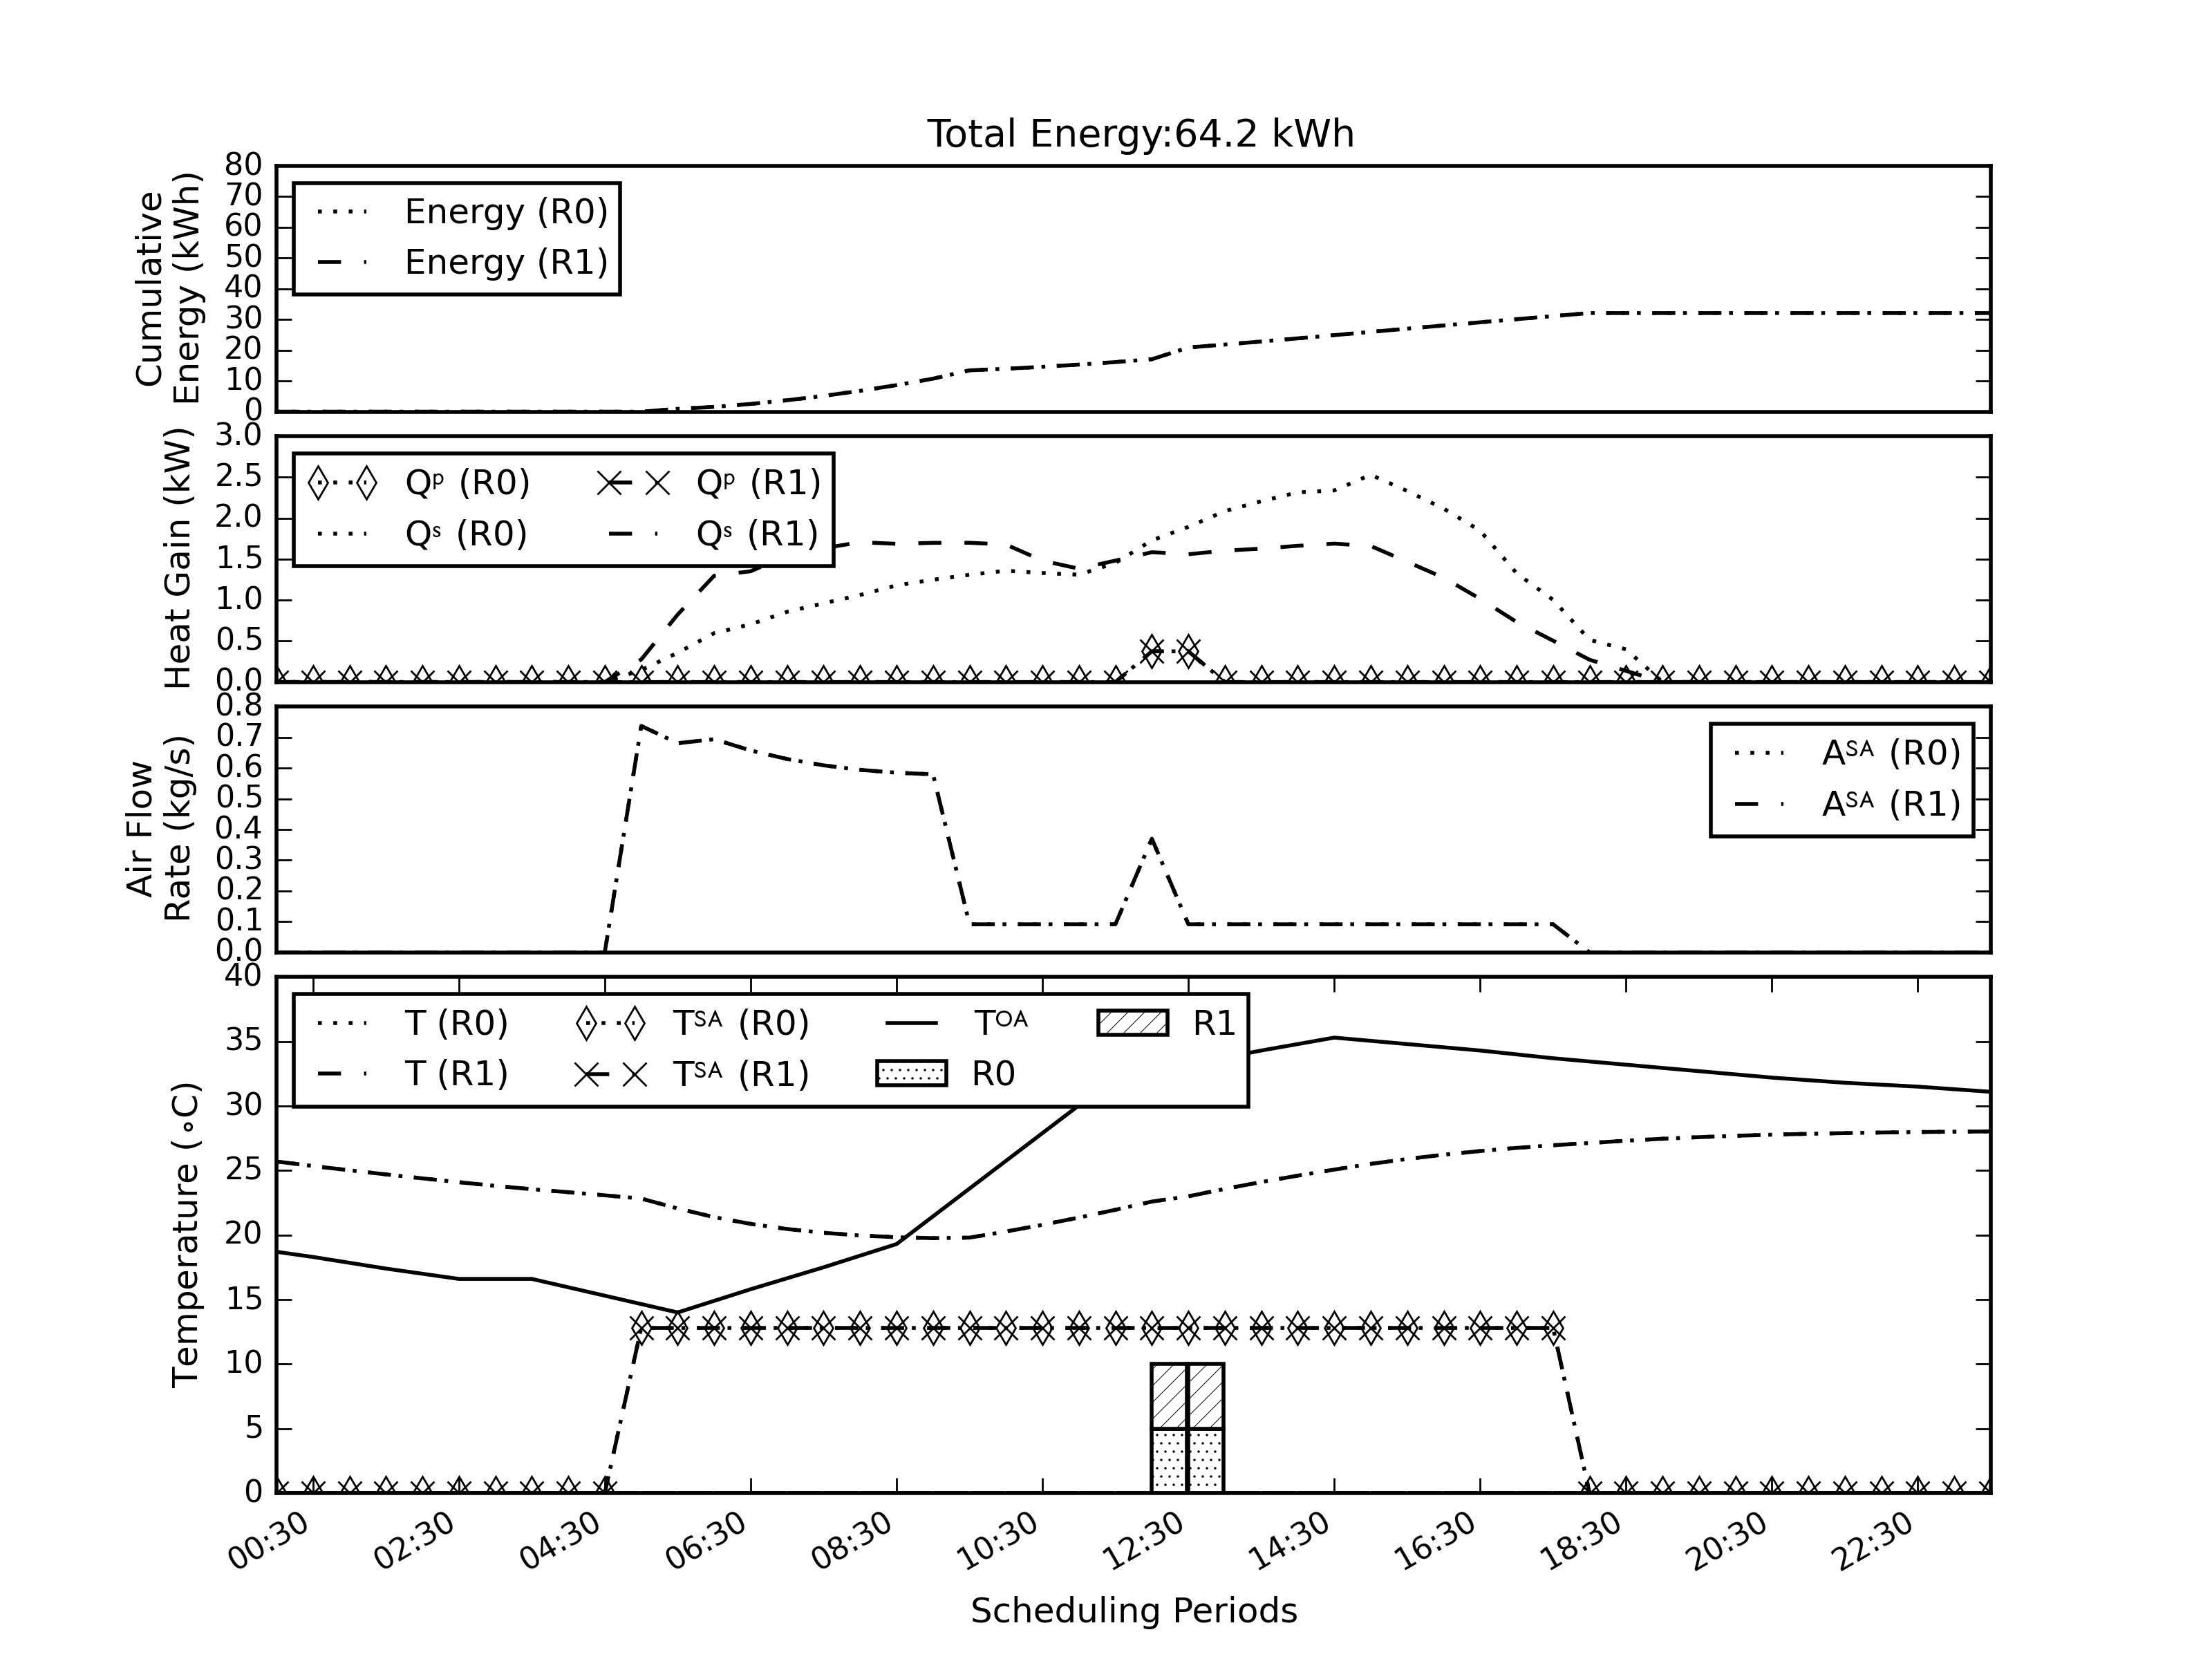
\includegraphics[width=0.9\linewidth]{figs/lrlc_opt_ws.png} \\
(a) Optimal Solution (OS) \\[6pt]
  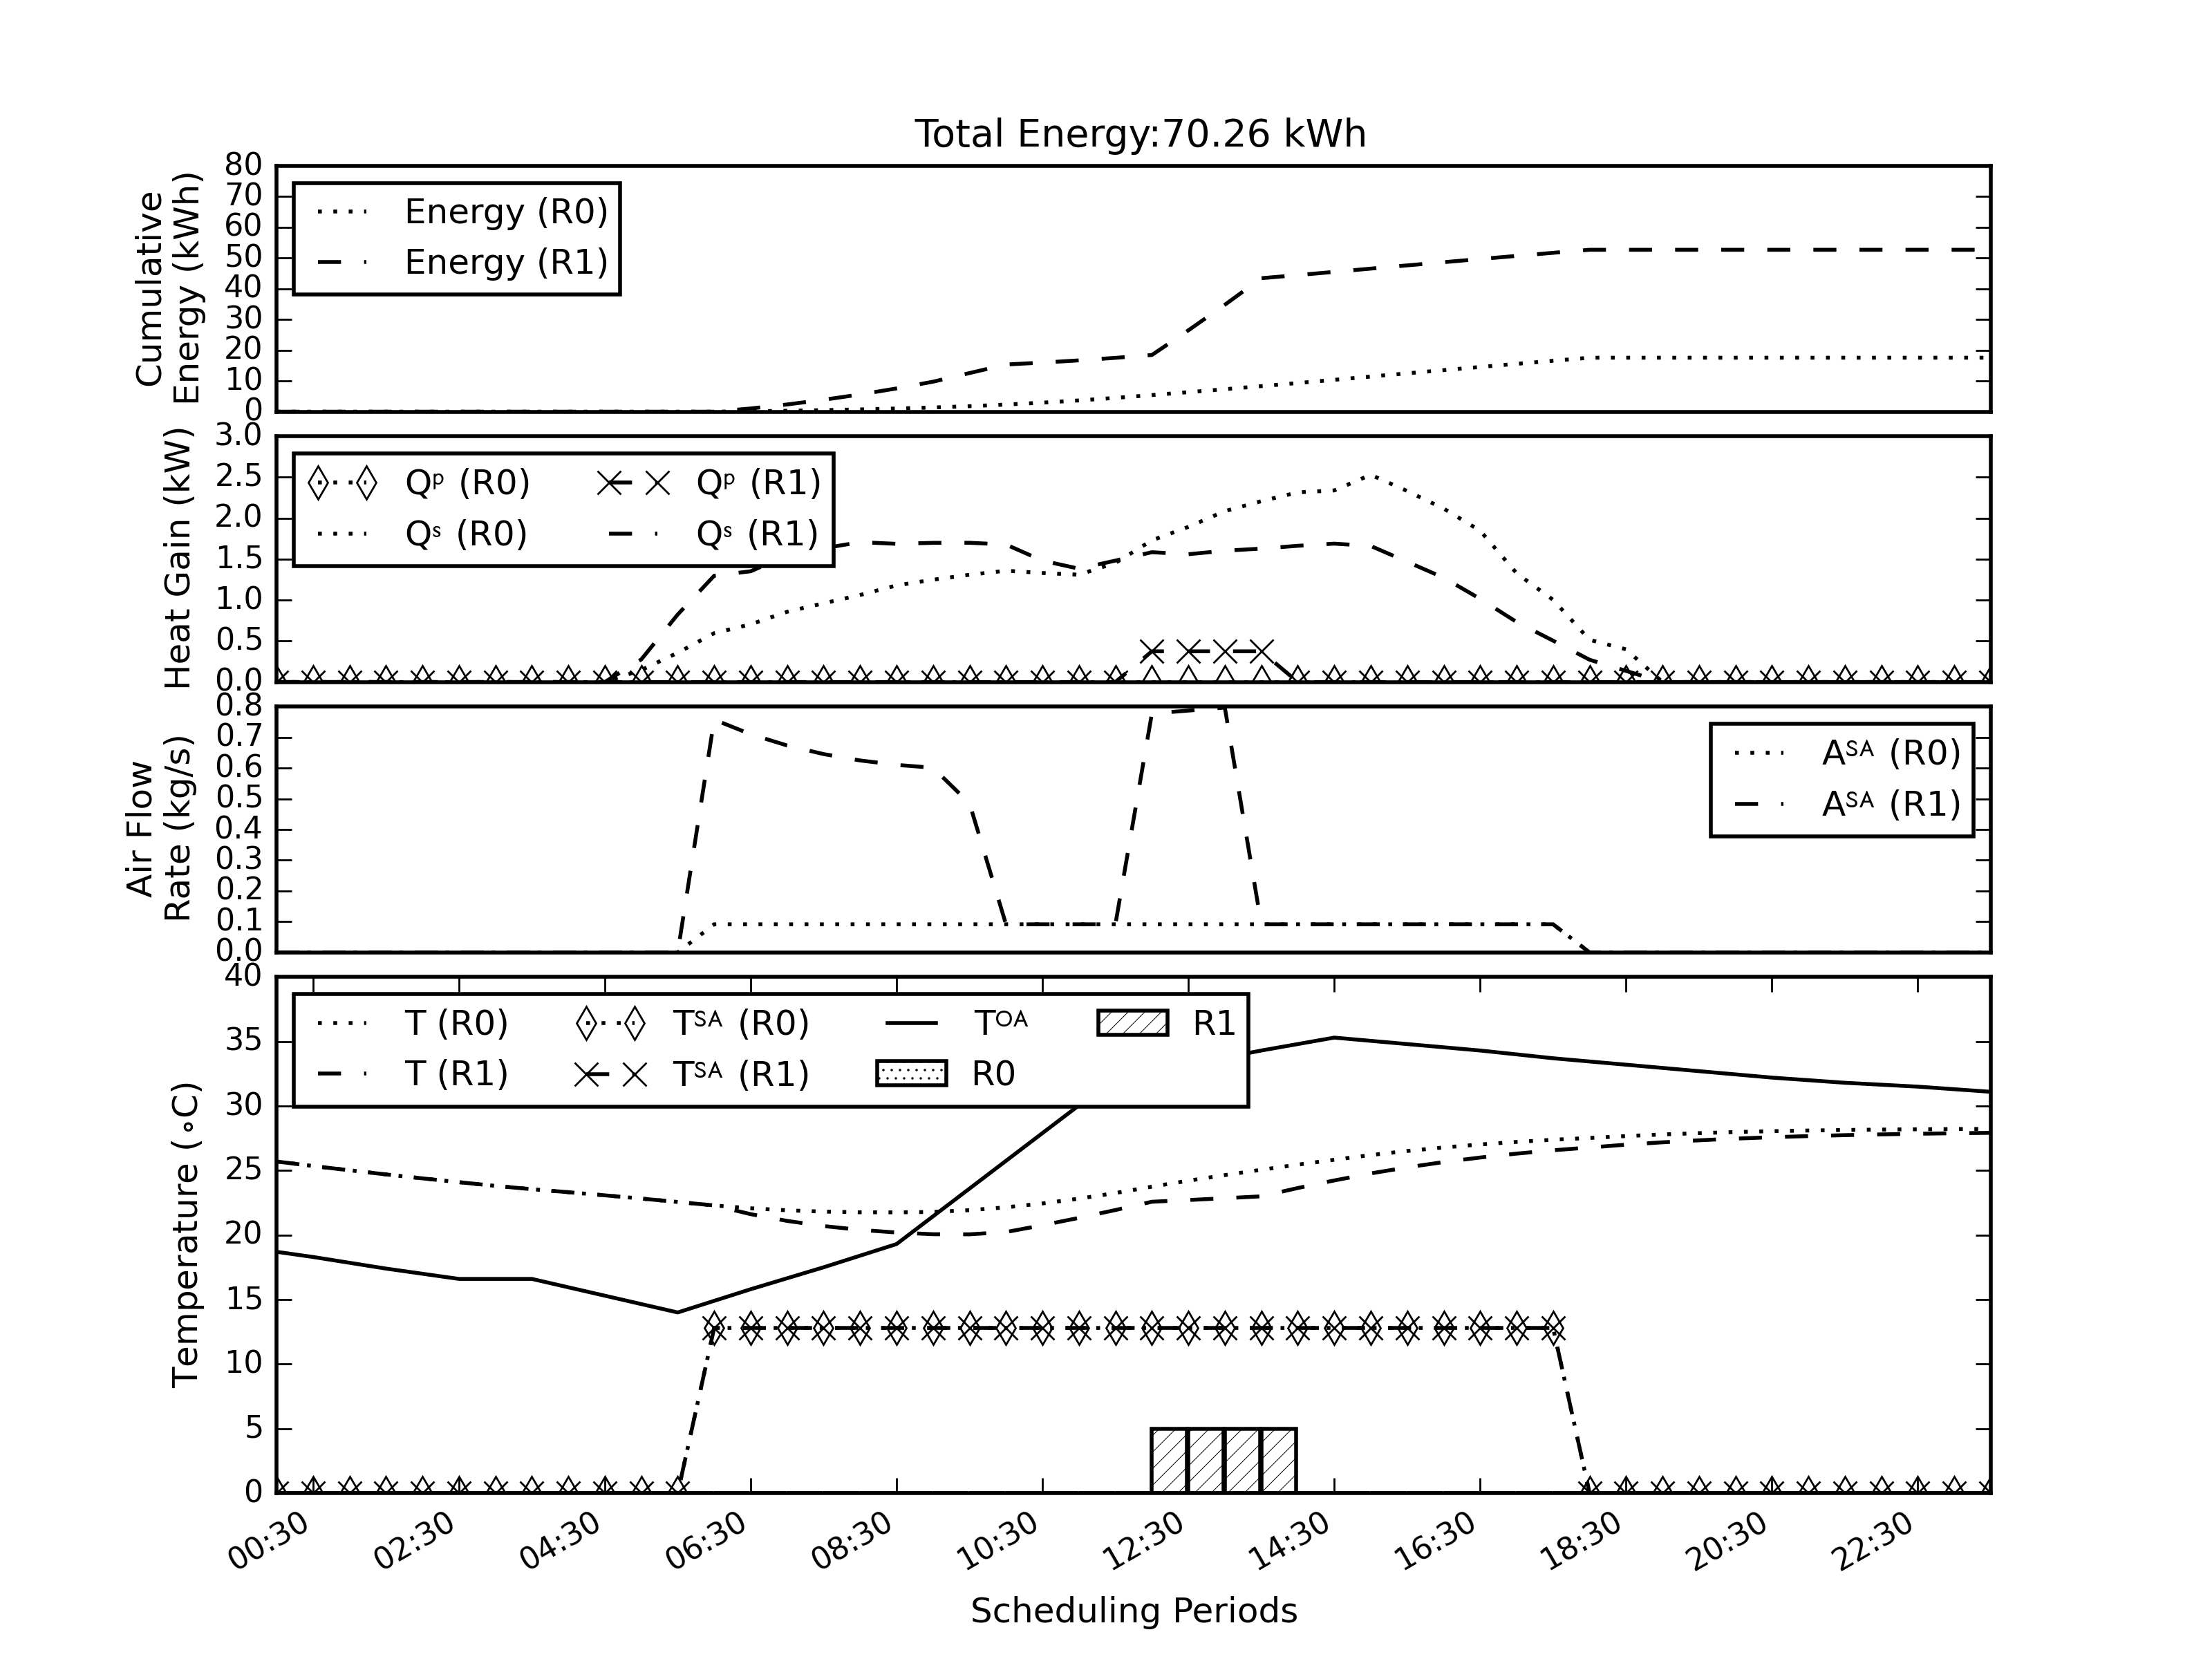
\includegraphics[width=0.9\linewidth]{figs/lrlc_b2b_ns.png} \\
(b) Back-to-back Heuristic-based Solution (HN) \\[6pt]
\end{tabular}
\caption{HVAC control with different scheduling approaches}
\label{fig:mip_scheap}
\end{figure}

Figure \ref{fig:mip_scheap} shows the results using both schemes. With our OS approach, the HVAC is turned on at 05:00 in the morning to cool down the room using the outdoor cold air. The meetings are scheduled in parallel at 12:00-13:00 as the cost of energy consumption is identified as optimal with such setting. Given both rooms being pre-cooled, the amount of outdoor air required to maintain the zones' temperature are approximately 0.36 kg/s between 12:00 to 12:30. On the other hand, using the HN approach, the HVAC is only activated at 06:00 and the meetings are forced to be scheduled in the same room. Although room R1 has been pre-cooled prior to the meetings (from 06:00 to 10:00), approximately 0.7 kg/s outdoor air are still required to be pushed into the room between 12:00 to 13:30 to maintain the zone temperature. In this simple scenario, our joint model achieves 6 kWh savings compared to the heuristic approach. We show that the heuristics of scheduling activities back-to-back in the same room in order to leverage thermal inertia does not necessary lead to energy savings.

% say thermal inertia not necessary effective
% HN: to 12.8$^\circ$C at 12:00 to 13:30 when the external temperatures are between 32$^\circ$C-34$^\circ$C.

\subsubsection{Experiment Results} 

To examine problems with different degree of constrainedness, we extracted 70 problem instances from the PATAT dataset, consisting of 
40 instances of 10 meetings each, 20 instances of 20 meetings each, and 10 instances of 50 meetings each. All meetings have up to 30 attendees, a 1.5h duration and an allowable time range of one or two random days (09:00-17:00) within the 5 days of the experiment.

The AN/AS results are obtained by selecting, for each instance, an arbitrary schedule consistent with the scheduling Constraints \eqref{eq:ms_every}-\eqref{eq:ms_meeting} in Section~\ref{sec:mip:scheduling} and using it as input to the occupancy-based HVAC control model in Section~\ref{sec:mip:control}. Similarly, the HN/HS results are obtained by selecting the schedule optimising the heuristic among those consistent with the scheduling constraints, and using it as input to the occupancy-based HVAC control model. The ON/OS results are obtained by solving the joint model for each instance.


%Conventional	522.86	Baseline	330.90
%AN	212.14	40.57	74.83
%AS	199.94	38.24	64.78
%HN	184.26	35.24	51.85
%HS	177.32	33.91	46.13
%ON	124.13	23.74	2.30
%OS	121.34	23.21	Baseline

\begin{table}[t]
\centering
\begin{tabular}{p{0.1\linewidth} p{0.25\linewidth} p{0.25\linewidth} p{0.25\linewidth}}
\hline \centering{Strategy}  & \centering{Avg. energy consumption (kWh)} &  \centering{\% Consumption vs. CO} &  \centering{\% Excess Consumption vs. OS} \tabularnewline
\hline \centering{CO}  & \centering{522.86} &  \centering{Baseline} & \centering{330.9\%} \tabularnewline
\hline \centering{AN}  & \centering{212.14} &  \centering{40.57\%} &  \centering{74.84\%}\tabularnewline
\hline \centering{AS}  & \centering{199.94} &  \centering{38.24\%} &  \centering{64.78\%}\tabularnewline
\hline \centering{HN}  & \centering{184.26} &  \centering{35.24\%} &  \centering{51.86\%}\tabularnewline
\hline \centering{HS}  & \centering{177.32} &  \centering{33.91\%} &  \centering{46.14\%}\tabularnewline
\hline \centering{ON}  & \centering{124.13} &  \centering{23.74\%} &  \centering{2.30\%}\tabularnewline
\hline \centering{OS}  & \centering{121.34} &  \centering{23.21\%} &  \centering{Baseline} \tabularnewline
\hline
\end{tabular}
	\caption{Comparison of conventional approach (CO) with arbitrary (A), heuristic (H), and optimal (O) scheduling strategies over HVAC with (S) and without (N) standby mode.}
	\label{tab:sche_e}
\end{table}

\begin{table}[t]
\centering
\begin{tabular}{p{0.1\linewidth} p{0.12\linewidth} p{0.12\linewidth} p{0.12\linewidth} p{0.12\linewidth} p{0.12\linewidth} p{0.12\linewidth}}
\hline \centering{Strategy}  & \multicolumn{3}{c}{Avg. energy consumption (kWh)} &  \multicolumn{3}{c}{\% Excess Consumption vs. OS} \tabularnewline
\hline \centering{Meetings}  & \centering{10} &  \centering{20} & \centering{50} &  \centering{10} & \centering{20} & \centering{50} \tabularnewline
\hline \centering{AN}  & \centering{163.8} & \centering{219.8} & \centering{380.0} & \centering{64\%}  & \centering{95\%} & \centering{70\%} \tabularnewline
\hline \centering{AS}  & \centering{154.2} & \centering{206.0} & \centering{361.4} & \centering{55\%}  & \centering{83\%} & \centering{62\%}\tabularnewline
\hline \centering{HN}  & \centering{142.5} & \centering{178.8} & \centering{355.6} & \centering{43\%}  & \centering{59\%} & \centering{59\%}\tabularnewline
\hline \centering{HS}  & \centering{137.8} & \centering{172.0} & \centering{340.1} & \centering{38\%}  & \centering{53\%} & \centering{52\%}\tabularnewline
\hline \centering{ON}  & \centering{100.4} & \centering{115.8} & \centering{232.8} & \centering{0.8\%} & \centering{3\%}  & \centering{4\%}\tabularnewline
\hline \centering{OS}  & \centering{99.7}  & \centering{112.5} & \centering{223.4} & \multicolumn{3}{c}{Baseline} \tabularnewline
\hline
\end{tabular}
	\caption{A detailed breakdown by meeting size using different strategies.}
	\label{tab:sche_e_breakdown}
\end{table}

Table~\ref{tab:sche_e} shows, for each of the 6 approaches, the average energy consumption per room over the 70 instances, and the percentage of consumption taking the conventional approach (CO) as the baseline. Table~\ref{tab:sche_e_breakdown} provides a detailed breakdown by meeting size. The results show a clear improvement as we move from arbitrary schedules (AN/AS), that are currently the norm with room booking systems, to energy aware schedules (HN/HS), and a much greater improvement when these  schedules take into account the capabilities of occupancy-based HVAC control (ON/OS). Specifically, the ON/OS approaches consume only 23\% of the conventional approach, and are 50\%-70\% better than the state-of-the-art approaches. The interactions between the various scheduling constraints, the thermal dynamics of the building and the HVAC control are so complex that heuristic methods can only achieve a fraction  of the performance of the global optimisation methods enabled by our MILP model.  As expected, the gain conferred by the standby mode  decreases as we move to schedules that make better time and location decisions. Similarly, we observed that for more constrained problems (e.g. with 50 meetings), the standby mode is more effective, because there is a greater likelihood that meetings need to be scheduled in rooms that require higher cooling load which the standby mode can mitigate by pre-cooling.


\section{Related Work}
\label{sec:mip:related}

Occupancy information, knowing whether or not there are people in a room and ideally also knowing how many people there are in a room, is at the basis of moving away from schedule-based control towards occupancy-based control. Schedule-based control is inefficient as it operates HVAC systems according to a fixed schedule that often assumes maximum zone occupancy. Occupancy-based control, on the other hand, uses MPC approach and optimises HVAC control based on the detected or forecast occupancy information. \cite{klein2012coordinating} and \cite{oldewurtel2012use} take into account occupancy forecasts and weather to estimate energy saving opportunities. \cite{goyal2013occupancy} also take into account occupancy forecasts and compare the performance of MPC strategies with feedback controllers using occupancy measurements. \cite{mady2011stochastic} build occupancy model and use MPC to improve on energy efficiency while maximising occupant comfort. \cite{mamidi2012adaptive}, \cite{li2012measuring}, \cite{erickson2009energy} and \cite{agarwal2010occupancy} deploy sensors to detect real-time occupancy and use this information to control HVAC system in an adaptive manner. These previous works on occupancy-based HVAC control, also including works by \cite{brooks2015energy,mady2011stochastic,parisio2013randomized,xu2009model}, treat occupancy information as an input parameter and not as a control variable. Our work is different as it incorporates both HVAC control and occupancy scheduling into a unified model. In addition, our standby mode improves the feasibility and solution quality of model-predictive HVAC control methods. It is worth noting that the work on sensor-based occupancy detection approach complements our work, in which the detected occupancy information can be taken as an additional input into our model to reflect the actual occupancy flow in the buildings. 

%Their conclusion is that occupancy predictions can lead to additional energy savings over occupancy measurements especially when ventilation standards change. Currently the ASHRAE ventilation standard \cite{ashrae} requires that a certain amount of outside air is mixed with return air from the zones regardless whether a zone is occupied or not.

Various methods have been used to solve the non-linear non-convex optimisation problem in HVAC control. In \cite{klein2012coordinating}, the HVAC control is simplified to a linear model by assuming the supply air temperature is constant, thus forming a linear function to calculate only the supply air flow rate. \cite{oldewurtel2013importance} consider rather complex HVAC actuation including the control of blind positions, lighting, chiller, cooling tower, radiators etc. They apply sequential linear programming using MAP (Method of Approximation) programming \citep{griffith1961nonlinear} to linearise their HVAC model. \cite{ma2011distributed} solve the non-linear HVAC control constraints using dual decomposition and \cite{sun2010integrated} adopt lagrangian relaxation and dynamic programming using surrogate subgradient method. Some works \citep{wang2000model, xu2009model, mossolly2009optimal} implement genetic algorithms to search for optimal value of the supply air temperature and flow rate. In our work, we use McCormick's relaxation that guarantees to return an optimal lower bound on the objective function. The need to reduce computational effort and scalability of the joint model are our motivating factor to develop a linearised model for HVAC control. 

Much of the existing literature on energy-aware scheduling methods typically take advantage of thermal inertia using heuristics such as minimising the number of rooms used and/or assigning lower costs to meetings scheduled back to back in the same room \citep{pan2012thermal,kwak2013tesla,majumdar2012energy,chai2014minimizing}. An important limit of these works is that they all share a black-box modeling approach for calculating HVAC energy consumption. This black-box approach confines the search to a rather limited space that does not exploit the HVAC's full capabilities. Another limitation is the assumption of an anonymous list of meeting participants, which ignores the existence of meeting conflicts and the fundamental need for resolving them. 

\cite{kwak2013tesla} analyse the impact of scheduling flexibility on energy savings, based on the historical data of a conventional HVAC control approach. Although we have not quantified explicitly, our experiments suggest that occupancy-based HVAC control helps to mitigate the impact of less flexible scheduling requests. However, in future, it would be interesting to study the tradeoff between scheduling flexibility versus HVAC control. For example, with occupancy-based control, what is the minimum scheduling flexibility required to achieve the same energy savings, compared to conventional HVAC control with some scheduling flexibility? Such study is interesting as it allows us to quantify the difference in terms of energy gain, given the ability to manipulate the HVAC operations, the flexibility to schedule meeting requests, or both.

There has been a significant amount of work that focuses on meeting scheduling \citep{modi2004multiagent,refanidis2010constraint,tran2016smart} and timetabling \citep{merlot2002hybrid,di2002multi,abdullah2007tabu}. Our work differs from these established field by adding an additional objective to conserve energy in the buildings where these activities are held. 

Energy-oriented scheduling has gained more attention in recent years due to the significant cost saving opportunities. 
\cite{ifrim2012properties} present a MIP-based energy-price savings scheduling model to reduce cost in production scheduling. \cite{dupont2012energy} use CP to develop an energy aware framework for virtual machine placement in cloud-based data centers. \cite{scott2013residential} describe an online stochastic MILP to schedule home appliances based on real-time pricing. \cite{ono2012risk} develop a HVAC control approach that integrates with occupant activities scheduling and blind control in a smart home.  Most works focus on energy-aware scheduling in production lines, data centers and residential buildings whilst our work specifically targets energy-efficient scheduling in commercial offices and university buildings, where HVAC consumption dominates the building's energy consumption. 



\section{Conclusion and Future Work}
\label{sec:mip:conclusion}

In this work we focus on meeting scheduling, as meeting scheduling is one practical approach to strategically control occupancy flows and optimise HVAC utilisation. However, our model is more broadly applicable to scheduling occupant activities within specified time windows, and ultimately, can be integrated into a range of room booking and scheduling systems. To bring awareness of the capabilities of the building's HVAC system to the scheduling process, we solve a joint HVAC control and occupancy scheduling problem. This problem involves determining the times and locations of a set of meetings, as well as the supply air temperature and air flow rate for  each building zone, so as to minimise HVAC consumption. Existing approaches solve the HVAC control problem and the occupancy scheduling problem in isolation. While the joint problem is more challenging, it does achieve a much higher rate of energy savings. 

Directions for future work include extending our model to include more HVAC parameters such as humidity, return air ratio, damper control and conditioned air temperature. This involves the modeling of chiller and boiler operations on the supply side of the HVAC system. A more comprehensive HVAC model helps to improve the accuracy of HVAC control and the prediction of energy consumption in buildings. In addition, further research is needed to learn and improve the building thermal dynamics model using real data. Specifically, the RC parameters can be calibrated based on temperature data collected from actual buildings using machine learning techniques. 

We are also interested in exploring the CP formulation of joint HVAC control and meeting scheduling. As the joint model consists of hybrid discrete-continuous variables, we will reformulate it by discretizing the HVAC control variables, and compare the solution quality generated by both MIP and CP models. 

%In the coming chapters, we show how our joint model can be scaled to solve larger problems and handle impromptu meeting requests in real-time.


% - Warm start NLP with LP model?


%These equations form a system of nonconvex non-linear constraints, which constitute a challenge when embedded in optimisation problems. convex quadratic relaxation of the HVAC control equations that is easily embedded in MIP.

%Adding humidity --> 
%Multilinear expressions have been extensively studied in
%the literature and corresponding convex envelopes are well-defined in some
%cases. For bilinear expressions, convex envelopes were introduced by McCormick
%in [37,4] (Figures 2(a) and 2(b)) Multilinear terms such as vivjvk are relaxed
%using a sequential bilinear approach. The trilinear envelopes introduced by [38,
%39] were also considered. Nevertheless, on all applications of interest, numerical
%experiments have shown that the sequential McCormick relaxation offers
%comparably tight bounds.






%TODO:  
%  (from data) say how many times destroy and reconstruct, average how many rooms were destroyed.
%	 Add dollar graphs

%  Add experimental results using different neighbourhoods
%  Add concept of LNS, symmetry
%     Say today solver such as cplex, gurobi can do symmetry detection, however it is more effective by leveraging on knowledge on problem structure
%  Add SMAC - how smac works and other parameter tuning software
%  Add different way of neighourhood...say pros and cons



%%%%

%%%%


\chapter{Scaling to Large Problems}
\label{cha:lns}

\section{Introduction}

In Chapter~\ref{cha:milp} we showed that combining HVAC control with occupancy scheduling can lead to substantial improvements in energy efficiency. Our MIP-based joint model achieves a significant energy reduction when compared to the existing state-of-the-art approaches \citep{goyal2013occupancy,kwak2013tesla,majumdar2012energy,chai2014minimizing}.
%those heuristic-based energy-aware scheduling approaches that assume a black-box model for HVAC control \citep{kwak2013tesla,majumdar2012energy,chai2014minimizing}. 
Given the highly-constrained nature of occupancy scheduling with HVAC control, solving the integrated problem as a MIP seems to be a reasonable choice. MIP easily manages the interaction between occupancy scheduling and the impact it has on HVAC energy consumption. The problem with the MIP-based approach, however, is that it does not scale. It only allows us to solve small problem instances in reasonable time. 

In Chapter \ref{cha:milp} Section \ref{sec:mip:experiments}, the largest instances we tackle consist of 4 rooms and 50 meetings over 5 days. When the problem size increases to a larger number of rooms and number of meetings, for example 20 rooms and 200 meetings, MIP's convergence becomes very slow and sometimes fails to occur after a day. This is a common problem in a MIP model involving symmetry. Symmetry exists in a MIP model when integer variables can be permuted without changing the structure of the problem \citep{margot2010symmetry}. This property greatly affects the branch-and-bound process in MIP. 
Technically, symmetries can be removed effectively by taking advantage of a problem structure. This includes grouping the variables with identical properties into one group or imposing an ordering to the variables by lexicographic constraints.
% or leveraging on the structure of the problem and introducing symmetry breaking constraints (eg. impose an ordering to the variables by introducing lexicograpic constraints). 
This is a technique regarded as \textsl{symmetry breaking}\footnote{Most of the existing optimisation solvers \citep{gurobi, cplex2009v12} also support problem-independent symmetry breaking technique, which solely depend on the MIP model. They provide a configurable parameter that activates automatic detection and removal of symmetries in MIP. However, it is stated at \cite{gurobisym} that changing the value of this parameter rarely produces a significant benefit.}. In our model, a large number of 
\vspace*{-2px}
\begin{enumerate}
	\item meetings with similar properties (eg. number of attendees, meeting time windows, room capacity, equipments required etc.),    \label{sym1} 
	\item rooms with similar temperature and temperature fluctuation rates, and  \label{sym2}
	\item scheduling periods with low diurnal temperature variation.  \label{sym3}
\end{enumerate}
\noindent form symmetries or near-symmetries that lead to slow convergence. 
The first type of symmetries \eqref{sym1} can be tackled using the grouping approach. These are common in scheduling problems, where many meetings (a.k.a jobs) have identical properties. To overcome this, we can reformulate the model so that these meetings with similar properties are grouped, thus exploiting the symmetries in \eqref{sym1}. Unfortunately, for symmetry types \eqref{sym2} and \eqref{sym3}, as the rooms temperatures fluctuate according to occupancy, two rooms with similar properties may have different temperatures depending on the scheduled meeting allocations, hence resulting in an asymmetrical state. Therefore it is impossible to group them into one room type. This leads to multiple symmetric optima with very small differences that renders branch-and-bound in MIP ineffective. The latter is in fact a ''near-symmetric`` problem that cannot be solved effectively via symmetry breaking, and has been an open problem in MIP for a long time \citep{ostrowski2010symmetry}. Fortunately, given the detailed understanding of the HVAC control and occupancy scheduling problem, it is possible to exploit the model structure to overcome these issues. 

In this chapter, we adopt a hybrid solution that combines MIP with large neighbourhood search (LNS) to solve our joint control and scheduling problem. The advantage is twofold. This strategy copes with symmetries and near-symmetries in a MIP-based system based on our understanding on the problem structure. It also scales our joint model to handle problem sizes that, for example, companies and universities may face when scheduling meetings and lectures. A commercial office or an university building typically consists of multiple floors with a lot of rooms. In order to consolidate energy-efficient schedules, a meeting appointment or an university timetabling application needs handle large number of activities across these rooms. For example, about 300 meetings have to be scheduled every weekday across 35 study rooms in the main library of University Southern California \citep{kwak2013tesla}. These bookings are handled by a centralized online room reservation system. Meanwhile, night and weekend classes were consolidated from 21 buildings to 5 buildings in \cite{portland:2012} to reduce energy consumption. Thus, it is crucial for our joint model to handle these large instances and produce near-optimal control and scheduling solutions, given sets of activity requests with different constrainedness and sets of buildings with varying thermal response.

We extend our work in Chapter \ref{cha:milp} and develop an approach that scales to larger problems by combining MIP with LNS. LNS is used to destroy part of the schedule and MIP is used to repair the schedule so as to minimise energy consumption. This approach is far more effective than solving the complete problem as a MIP problem. Our results show that solutions from the LNS-based approach are up to 36\% better than the MIP-based approach when both are given 15 minutes. 

The remainder of this chapter is organized as follows. 
Section \ref{sec:lns} describes the LNS model. We discuss in turn our LNS algorithm, the formulation of initial solution, the destroy and repair steps, and finally the LNS parameter tuning. 
Section \ref{sec:lns_mip} highlights the MIP model formulation for the LNS initialization stage and the MIP model reduction to remove symmetries and speed up our joint model. 
We present our experimental results in Section \ref{sec:results} and review the related work in Section \ref{sec:related_work}.
Finally, we conclude with key observations and opportunities for further work in Section \ref{sec:lns:conclusion}.

%---------------------------------
\section{Large Neighborhood Search}\label{sec:lns}

LNS is a local search metaheuristic, which was originally proposed by \cite{shaw1998using}. In LNS, an initial solution is improved iteratively by alternating between a destroy and a repair step. The main idea behind LNS is that a large neighbourhood allows the heuristic to easily navigate through the solution space even when the problem is highly-constrained. This is opposed to a small neighbourhood, which may make escaping a local minimum much harder. Algorithm \ref{alg:lns} outlines our LNS approach. 

\begin{algorithm}[ht!]
\small
%\SetAlgoLined
\SetKwFunction{Return}{return}
\SetKwInput{Input}{Input}
\SetKwInput{Output}{Output}
\SetKwInput{Initialize}{Initialization}
\SetKwInput{Algorithm}{Destroy \& Repair}
\SetKwIF{If}{ElseIf}{Else}{if}{then}{else if}{else}{endif}
 \Indm
 \Input{Meeting requests $M$, Rooms $L$, time steps $K$}
 \Output{Master Schedule $S$, Energy Consumption $J$ }
 \Initialize{}
 \Indp{$S \gets \emph{GenInitialMeetingSchedule}(M, L, K)$\\
$ J \gets \emph{GenHVACControl}(S)$
 }\\
 \Indm
 \Algorithm{}
 \Indp
 \While{not LnsTimeUp()}
 {
	$L' \gets \emph{SelectNeighborhood}\left(L\right)$ \\
	$\emph{DestroyNeighborhood}\left(S, M(L'), L' \right)$ \\
	$\langle S', J' \rangle \gets \emph{RepairNeighborhood}\left(S, M(L'), L' \right)$\\
	\If{$J' < J$}	
	{
		$J \gets J' $\\
		$\emph{UpdateSchedule}\left(S', S \right)$
	}
 }
 \Return $S$
 \caption{LNS approach}
 \label{alg:lns}
\end{algorithm}

\subsection{Initialization Phase}\label{sec:lns_init}

Our LNS approach starts with an initial feasible solution, which is generated using a greedy heuristic. First, this heuristic finds a feasible meeting schedule by minimising the number of rooms in which meetings are located. As we saw in Chapter \ref{cha:milp}, this is a commonly used heuristic in energy-aware meeting scheduling. Second, it determines the HVAC control settings of supply air temperature and supply air flow rate to minimise energy consumption given the fixed schedule. This two-stage approach allows us to come up with an initial solution in reasonable time.


\subsection{Destroy \& Repair}\label{sec:lns_dr}

Next, we run multiple iterations of destroy and repair steps to re-build and re-optimise the selected neighbourhoods. An important decision in the destroy step is determining the amount of destruction. If too little is destroyed the effect of a large neighbourhood is lost, but if too much is destroyed then the approach turns into repeated global re-optimisation. As for the repair step, an important decision is whether the repair should be optimal or not. An optimal repair will typically be slower than a heuristic, but may potentially lead to high quality solutions in a few iterations. As a result, a neighbourhood destroy and repair strategy is essential in achieving good performance overall.

Our LNS approach considers a room-based neighbourhood that contains a subset of the rooms or zones. In particular, we destroy the schedule in two to four randomly selected rooms. This forms a subproblem that can be solved effectively using MIP. When destroying meetings in more than four zones, MIP performance can degrade very quickly and even solving the linear programming relaxation can become quite time consuming. The repair consists in solving an energy aware meeting scheduling problem that is much smaller than the original problem. We do, however, limit MIP runtime to avoid excessive search during a repair step, and to avoid any convergence issues of the MIP problem. Setting a limit on runtime means that we do not necessarily solve the subproblem to optimality, but given that MIP solvers are anytime algorithms, we do improve solution quality in many of the LNS iterations. If we find an improved solution, then the new schedule and control settings are accepted. Otherwise, we maintain the solution that was just destroyed. Given that the LNS starts with a feasible solution and does not accept infeasible solutions, the solution remains feasible throughout the execution of the algorithm.

We should note that we have experimented with a variety of neighbourhoods. These include: destroying all meetings in randomly selected time steps, a combination of destroying all meetings in randomly selected rooms and time steps, and simply destroying a set of randomly selected meetings. Our observation was that none of these neighbourhoods performed as well as destroying all meetings in a number of randomly selected rooms. Destroying selected rooms means that meetings could be rescheduled at any time during the day. This allows the model to optimise supply air flow rate and supply air temperature over all the time steps. Destroying selected time steps means that meetings may switch rooms, but may need to be scheduled to the same time step due to time window restrictions. This limits the optimisation of supply air flow rate and supply air temperature due to the HVAC control constraints on neighboring time steps.

%There is a correlation between the time windows selected for HVAC control! Hence infeasible solution may happen... etc.


\subsection{LNS Parameter Tuning}\label{sec:lns_param}

In order to fine-tune the LNS heuristic we apply automatic parameter tuning, which is a useful step in producing better results on average.
The parameters that govern the behavior of the LNS heuristic are parameters determining the probability of destroying a number (2, 3, or 4) of rooms and the MIP runtime limit for the repair step. The probabilities on the number of rooms to destroy are defined as a 3-tuple with values ranging between [0,1] and the MIP runtime limit is a parameter with values ranging between 1 and 10 seconds. 

While it is possible to reason about certain parameters and their impact on overall performance, these parameters can take infinitely many values. Even though we consider only 4 parameters, it is impossible to try all possible configurations because of their continuous domains. Note, even with discretized domains with reasonable level of granularity it remains impractical to try out all configurations. As a result, we use the automated algorithm-configuration method called Sequential Model-based Algorithm Configuration (SMAC) \citep{hutter2011sequential} to optimise these parameters.

SMAC can be used to train parameters in order to minimise solution runtime, or to optimise solution quality. In our case, we fix the runtime and minimise energy consumption. We generate problem instances with different degrees of constrainedness and train the parameters to achieve the average best quality for all input scenarios.

Given a list of training instances and corresponding feature vectors, SMAC learns a joint model that predicts the solution quality for combinations of parameter configurations and instance features. This information is useful in selecting promising configurations in large configuration spaces. For each training instance we computed up to 17 features, including: 
\iffalse
(1) number of constraints, (2) number of variables, (3) number of non-zero coefficients, (4) number of meetings, (5) number of meeting types, (6) scheduling flexibility, (7) average duration of meetings, (8) number of meeting slots per day, (9) total number of meeting slots, (10)-(14) number of rooms in up to 5 building types, and (15)-(17) minimum, maximum, and average difference between outdoor temperature and temperature comfort bounds.
\fi
\begin{itemize}
\item number of constraints, 
\item number of variables, 
\item number of non-zero coefficients, 
\item number of meetings, 
\item number of meeting types, 
\item number of possible starting time slots (scheduling flexibility), 
\item average duration of meetings, 
\item number of meeting slots per day, 
\item total number of meeting slots, 
\item number of rooms in our 5 building types (defined in Chapter \ref{cha:milp}, Table \ref{tab:rc_wall_win}), and 
\item minimum, maximum, and average difference between outdoor temperature and temperature comfort bounds.
\end{itemize}
These features reflect problem characteristics and are used by SMAC to estimate performance across instances and generate a set of new configurations.

Given a list of promising parameter configurations, SMAC compares them to the current incumbent configuration until a time limit is reached. Each time a promising configuration is compared to the incumbent configuration, SMAC runs several problem instances until it decides that the promising configuration is empirically worse or at least as good as the incumbent configuration. In the latter case the incumbent is updated. In the end, the configuration selected by SMAC is generalized to all problem instances in the training set. For more details about SMAC, we refer readers to \cite{hutter2011sequential}.

%When the problem only involves a small number of rooms then IP can be quite effective. We exploit this observation be\varphi\varphi\varphi\varphi\varphi

% Talk about using probability to decide whether to destroy 2, 3, or 4 rooms, instead of an arbitrary input.



\section{MIP Model}\label{sec:lns_mip}

In this section, we present our MIP formulations that are used with LNS. We first describe the MIP model that generates an initial feasible solution.  Then we present a reduced model that removes symmetries in meeting requests and simplifies the thermal dynamics model. This reduced model is adopted in the initialization phase, as well as the destroy and repair steps. At the end, we recap the equations that is used in each phase.

% Rewrite this... not only apply to initial phase of the lNS, also destroy and repair
%In this section, we present our MIP formulations for the\textcolor[rgb]{1,0,0}{ initial phase of the LNS}. We first describe the model that generates an initial feasible solution. Then we present a reduced model that removes symmetries in meeting requests and simplifies the thermal dynamics model. At the end, we recap the joint model that is used in the destroy and repair steps.

\subsection{Initialization Phase}

%we present our MIP formulations for the\textcolor[rgb]{1,0,0}{ initial phase of the LNS}.
%Our goal is to generate an initial feasible solution as quickly as possible. This can be achieved by first generating a valid schedule, i.e. a schedule where all meetings are assigned and none of the scheduling constraints presented in Section \ref{sec:mip:scheduling} are violated. Instead of randomly assigning meetings to any room (while obeying all constraints), we adopt a heuristic by scheduling these meetings in minimum number of rooms at each day across the scheduling period. Thus, the objective function is defined as minimising the room used per day. Let $d = \left\{1,...,D\right\}$ be a set of day across the scheduling period with $D$ days. Let $K_d = k_{(d-1) \times N},...,k_{d \times N-1}$ be an ordered set of time steps belongs to day $d \in D$, $N$ is a constant denoting the total time slot per day (in our case, N=48) and $K_d \subseteq K$. The objective function is defined as 

Our goal is to generate an initial feasible solution as quickly as possible. This can be achieved by first generating a valid schedule, i.e. a schedule where all meetings are assigned and none of the scheduling constraints presented in Section \ref{sec:mip:scheduling} are violated. Instead of randomly assigning meetings to any room (while obeying all constraints), we adopt a heuristic that schedules these meetings in the minimum number of rooms each day across the scheduling period. Let D be the set of days across the scheduling period. Moreover, let $\func{day-of}: K \rightarrow D$ be the function giving the day in which time step $k$ starts, i.e. $\func{day-of}(k) = ((k-1) \div N) +1$, where $N$ is the number of time steps per day and $\div$ is the integer division. The objective function is defined as


%BAV_y_LD_0_1 + BAV_y_LD_0_2 + BAV_y_LD_0_3 + BAV_y_LD_0_4
   %+ BAV_y_LD_0_5 + BAV_y_LD_1_0 + BAV_y_LD_1_1 + BAV_y_LD_1_2
   %+ BAV_y_LD_1_3 + BAV_y_LD_1_4 + BAV_y_LD_1_5 + BAV_y_LD_2_0
   %+ BAV_y_LD_2_1 + BAV_y_LD_2_2 + BAV_y_LD_2_3 + BAV_y_LD_2_4
   %+ BAV_y_LD_2_5 + BAV_y_LD_3_0 + BAV_y_LD_3_1 + BAV_y_LD_3_2
   %+ BAV_y_LD_3_3 + BAV_y_LD_3_4 + BAV_y_LD_3_5
\begin{equation} \label{eq:objective_minr}
\mbox{minimise: } \sum_{l \in L, d \in D} y_{l,d}
\end{equation}

\noindent where,
% CSTR_MinRoom_MLK_0_0_210: BDV_x_MLK_0_0_210 - BAV_y_LD_0_4 <= 0
% CSTR_MinRoom_MLK_0_0_211: BDV_x_MLK_0_0_211 - BAV_y_LD_0_4 <= 0
% CSTR_MinRoom_MLK_0_1_210: BDV_x_MLK_0_1_210 - BAV_y_LD_1_4 <= 0
% CSTR_MinRoom_MLK_0_1_211: BDV_x_MLK_0_1_211 - BAV_y_LD_1_4 <= 0
% CSTR_MinRoom_MLK_1_1_162: BDV_x_MLK_1_1_162 - BAV_y_LD_1_3 <= 0
% CSTR_MinRoom_MLK_1_1_163: BDV_x_MLK_1_1_163 - BAV_y_LD_1_3 <= 0
\begin{equation} \label{eq:ms_minroomalloc} 
x_{m,l,k} \leq y_{l,d} \hspace{10pt} \forall m \in M, l \in L_m, k \in K_m, d = \func{day-of}(k)
\end{equation}

%\begin{equation} \label{eq:ms_minroomalloc} 
%x_{m,l,k} \leq y_{l,d} \hspace{10pt} \forall m \in M, l \in L_m, k \in K_m, d \in D_m
%\end{equation}

\noindent Recall that the variable $x_{m,l,k}$ equals to 1 if meeting $m$ is scheduled to start at time step $k$ in zone $l$ and equals to 0 otherwise. The binary variables $y_{l,d}$ determine if zone $l$ is being occupied in day $d$. Constraints \eqref{eq:ms_minroomalloc} set the value of $y_{l,d}$ to 1 when at least one meeting starts at zone $l$ at day $d$.

%\noindent Recall that the variable $x_{m,l,k}$ equals to 1 if meeting $m$ is scheduled to start at time step $k$ in zone $l$ and equals to 0 otherwise. The binary variables $y_{l,d}$ determine if zone $l$ is being occupied in day $d$. Constraints \eqref{eq:ms_minroomalloc} set the value of $y_{l,d}$ to 1 when at least one meeting starts at zone $l$ at day $d$. We let $D_m$ be the set of days that meeting $m$ can start, that is $D_m = \left\{D' \subseteq D | \forall k \in K_m, d \in D', k \in K_d\right\}$. 

With this, the initial schedule is generated by adding objective function \eqref{eq:objective_minr} and Constraints \eqref{eq:ms_minroomalloc} with Constraints \eqref{eq:ms_every}-\eqref{eq:ms_meeting} in Section \ref{sec:mip:scheduling}. Compared to randomly assigning meetings to any room, this approach packs as many meetings as possible in the same room at different day across the scheduling period. While scheduling meetings back-to-back does not necessary lead to an optimal solution, we recognize that it is a heuristic that generates a reasonably good initial solution for HVAC control. In the best case scenario, all meetings are assigned to the most energy-efficient room(s), and a good solution can be generated in the initial stage. To diversify the search space and avoid the worst case scenario where all meetings are assigned to a room that consumes a lot of energy, we bound these constraints in a daily basis so that meetings can be packed in different rooms at different days of the scheduling horizon. 

This initial schedule is then fed into our occupancy-based HVAC control model in Section \ref{sec:mip:control} to generate an optimal HVAC control setting. In this initialization phase, the first stage consists of an IP model where the decision variables are all integer variables. This model can be solved effectively using the state-of-the-art MIP solvers such as Gurobi \citep{gurobi}. 
Once the room and time allocations for all meetings have been identified, the second stage consists of a MIP model which need only optimise all continuous decision variables $a^{SA}_{l,k}$ and $T^{SA}_{l,k}$, and if standby mode is enabled, the binary variables $w_{l,k}$, for the HVAC control. As such, by decomposing the joint model into two-stages, our model can yield an initial solution quickly. 


\subsection{Model Reduction}

% Say Now we switch MIP formulation reduction, that apply to all MIP model in initial phase and destroy and repair steps...
In this section, we discuss two model reduction approaches that improve the performance of our MIP model. These approaches are applied to the MIP models in the initialization phase, as well as the destroy and repair steps. The resulting reduced model greatly improves the branch-and-bound of the MIP model, without compromising on the accuracy of the model.


\subsubsection{Removing Symmetries in Meetings}

\begin{figure}[b]
	\centering
		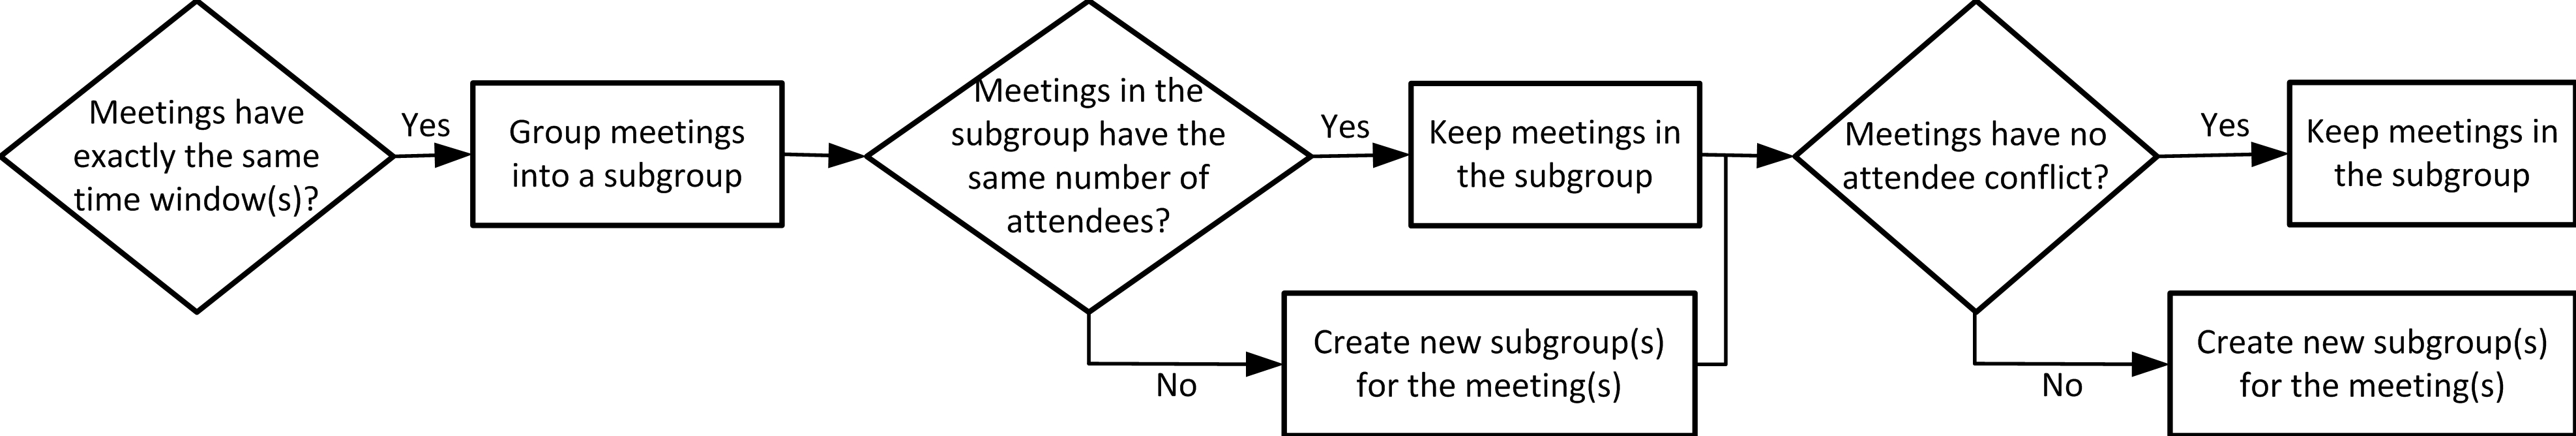
\includegraphics[width=1\linewidth]{figs/lns_mtype.jpg}
	\caption{The process flow of grouping identical meetings with similar properties.}
	%\vspace*{-2ex}
	\label{fig:mtype}
\end{figure}

One issue with the current model is that it can have a large number of equivalent solutions when two or more meetings are identical. In particular, let meetings 1 and 2 have the same time windows, same number of attendees, and no meeting conflicts. In this case, a solution in which $x_{1,l,k} = 1$ and $x_{2,l,k} = 0$ would be equivalent to one in which $x_{1,l,k} = 0$ and $x_{2,l,k} = 1$. In order to avoid the computational cost of generating both solutions we reduce the number of integer variables by defining meeting types. Meetings that are identical are considered to be of the same meeting type. Figure \ref{fig:mtype} illustrates the process flow of grouping meetings with similar properties into the same meeting type. Each subgroup represents a meeting type. Since the number of meeting types is smaller than the number of meetings, it allows for a simplified model that reduces symmetry. Without changing the model in its entirety we simply redefine $M$ to be the set of meeting requests and replace Constraint \eqref{eq:ms_every} with the one below to state that all meeting types must be scheduled $\psi_m$ times, where $\psi_m$ represents the number of meetings of type $m$.

\begin{equation} \label{eq:ms_everytype}
\mathop{\sum \limits_{l\in L_m, k \in K_m}} x_{m,l,k}= \psi_m \quad \forall m \in M
\end{equation}

%\noindent With constraints \eqref{eq:ms_everytype}, we remove the symmetries in meetings by grouping meetings of similar properties into single meeting type. 

\subsubsection{Simplifying The Building Thermal Dynamics Model}

The most involved constraints in the HVAC model come from modeling building thermal dynamics. In Section \ref{mip:thermal}, the temperature in a zone is affected by both internal and external walls. In our experiments, however, we observed that the temperature in a zone is mostly affected by the heat flow through external walls, the HVAC intervention and the occupants' heat load in the zone. The heat transfer from neighboring rooms through the internal walls is negligible based on our building settings. Hence, in our LNS model we only consider external walls, that is, those with that are outside facing. This approximation does not affect the HVAC control, hence it also does not impact the energy consumption, and therefore it does not impose any change to the schedule optimisation.
With this reduced model, the temperature constraints are simplified as follows:

\begin{equation}
\begin{split}
\begin{bmatrix}
\dot{T}_{l,k} \\
\dot{T}^{1}_{l,k} \\
. \\
. \\
\dot{T}^{N}_{l,k} \\
\end{bmatrix}
=
\begin{bmatrix}
-\frac{1}{\bm{C_l}} ( \sum_{n=1}^N \frac{1}{\bm{R_l^n}} + \frac{1}{\bm{R_l^w}}) & \frac{1}{\bm{C_l} \bm{R_l^1}} & . & . & \frac{1}{\bm{C_l} \bm{R_l^n}} \\
\frac{1}{\bm{C_l^1} \bm{R_l^1}} & -\frac{1}{\bm{C^1_l}} ( \frac{1}{\bm{R_l^1} + \bm{R_1^l}}) & 0 & 0 & 0 \\
. & . & . & . & .\\
. & . & . & . & .\\
\frac{1}{\bm{C_l^N} \bm{R_l^n}} & 0 & 0 & 0 & -\frac{1}{\bm{C^N_l}} ( \frac{1}{\bm{R_l^n} + \bm{R_N^l}})
\end{bmatrix}
\begin{bmatrix}
T_{l,k-1} \\
{T}^{1}_{l,k-1} \\
. \\
. \\
{T}^{N}_{l,k-1} \\
\end{bmatrix}
\\ +
\begin{bmatrix}
\frac{1}{\bm{C_l} \bm{R_l^w}} &
0 &
\frac{1}{\bm{C_l}}
\\
\frac{1}{\bm{C_l^1} \bm{R^l_1}} &
\frac{1}{\bm{C_l^1}} &
0 \\
. & . & . \\
. & . & . \\
\frac{1}{\bm{C_l^N} \bm{R^l_N}} &
\frac{1}{\bm{C_l^N}} &
0
\end{bmatrix}
\begin{bmatrix}
T^{OA}_{k-1} \\
Q^s_{l,k-1} \\
Q^p_{l,k-1}
\end{bmatrix}
+
\begin{bmatrix}
\frac{\Delta H^l_{k-1}}{\bm{C_l}} \\
0 \\
. \\
. \\
0
\end{bmatrix}
\end{split} \label{eq:roomtemperature_lns}
\end{equation}
%\begin{equation}
%Q^p_{l,k} = q^p pp_{l,k} \quad \forall l \in L, k \in K \label{eq:occupants}
%\end{equation}
%\begin{equation}
%\Delta H_{l,k} = C^{pa} a^{SA}_{l,k} (T^{SA}_{l,k} - T_{l,k}) \quad \forall l \in L, k \in K \label{eq:enthalpy}
%\end{equation}

Constraints \eqref{eq:roomtemperature_lns} model the temperature dynamics in zone $l$ when considering a room with $N$ external walls.  The expression $\dot{T}_{l,k} = \frac{T_{l,k} - T_{l,k-1}}{\bm{\Delta t}}$ is the rate of change in zone temperature and $\dot{T}^n_{l,k}$ is the rate of change in temperature of the external wall(s) $n = 1,..., N$. Recall that $\bm{C_l}$ and $\bm{C^N_l}$ respectively denote the thermal capacitance of zone $l$ and of the external wall $n$ in zone $l$. $\bm{R^n_l}$ and $\bm{R^w_l}$ respectively represent the thermal resistance of wall $n$ and the windows separating zone $l$ with the outdoors. $\bm{T^{OA}$} is the outdoor temperature, while $Q^s$ is the solar heat gain. With this, the building thermal dynamics model is obtained by adding equations \eqref{eq:roomtemperature_lns} with equations \eqref{eq:heatgain}, \eqref{eq:enthalpy}, \eqref{eq:tlf} and \eqref{eq:tlc}


\subsection{Summary of Model Equations}

\noindent \emph{GenInitialMeetingSchedule}. The initial schedule is generated by combining Equations \eqref{eq:objective_minr}, \eqref{eq:ms_minroomalloc}, \eqref{eq:ms_everytype}, and \eqref{eq:ms_totalalloc}-\eqref{eq:ms_meeting}.

\vspace{2pt}
\noindent \emph{GenHVACControl}.  The initial HVAC control is generated by adding Equations \eqref{eq:objective} - \eqref{eq:aSAT4}
with Equations~\eqref{eq:p_heat} and Equations~\eqref{eq:enthalpy} being linearised. Also, Equations \eqref{eq:roomtemperature}, \eqref{eq:temp:outer} and \eqref{eq:temp:inner} are replaced by \eqref{eq:roomtemperature_lns}. The result from the initial schedule, that is the values of $x_{m,l,k}$, is set as an input to this model. 

\vspace{2pt}
\noindent \emph{RepairNeighborhood}. The MIP model is formed by limiting $l$ to the selected neighbourood $L'$, and run the joint HVAC control and occupancy scheduling model by combining Equations \eqref{eq:objective}-\eqref{eq:hvac_standby_ASA}, \eqref{eq:roomtemperature_lns}, \eqref{eq:heatgain}-\eqref{eq:enthalpy}, \eqref{eq:tlf}-\eqref{eq:aSAT4}, \eqref{eq:ms_everytype}, \eqref{eq:ms_totalalloc}-\eqref{eq:ms_meeting}.


\section{Experiments}\label{sec:results}

\subsection{MIP vs. LNS}

\begin{figure}
	\centering
		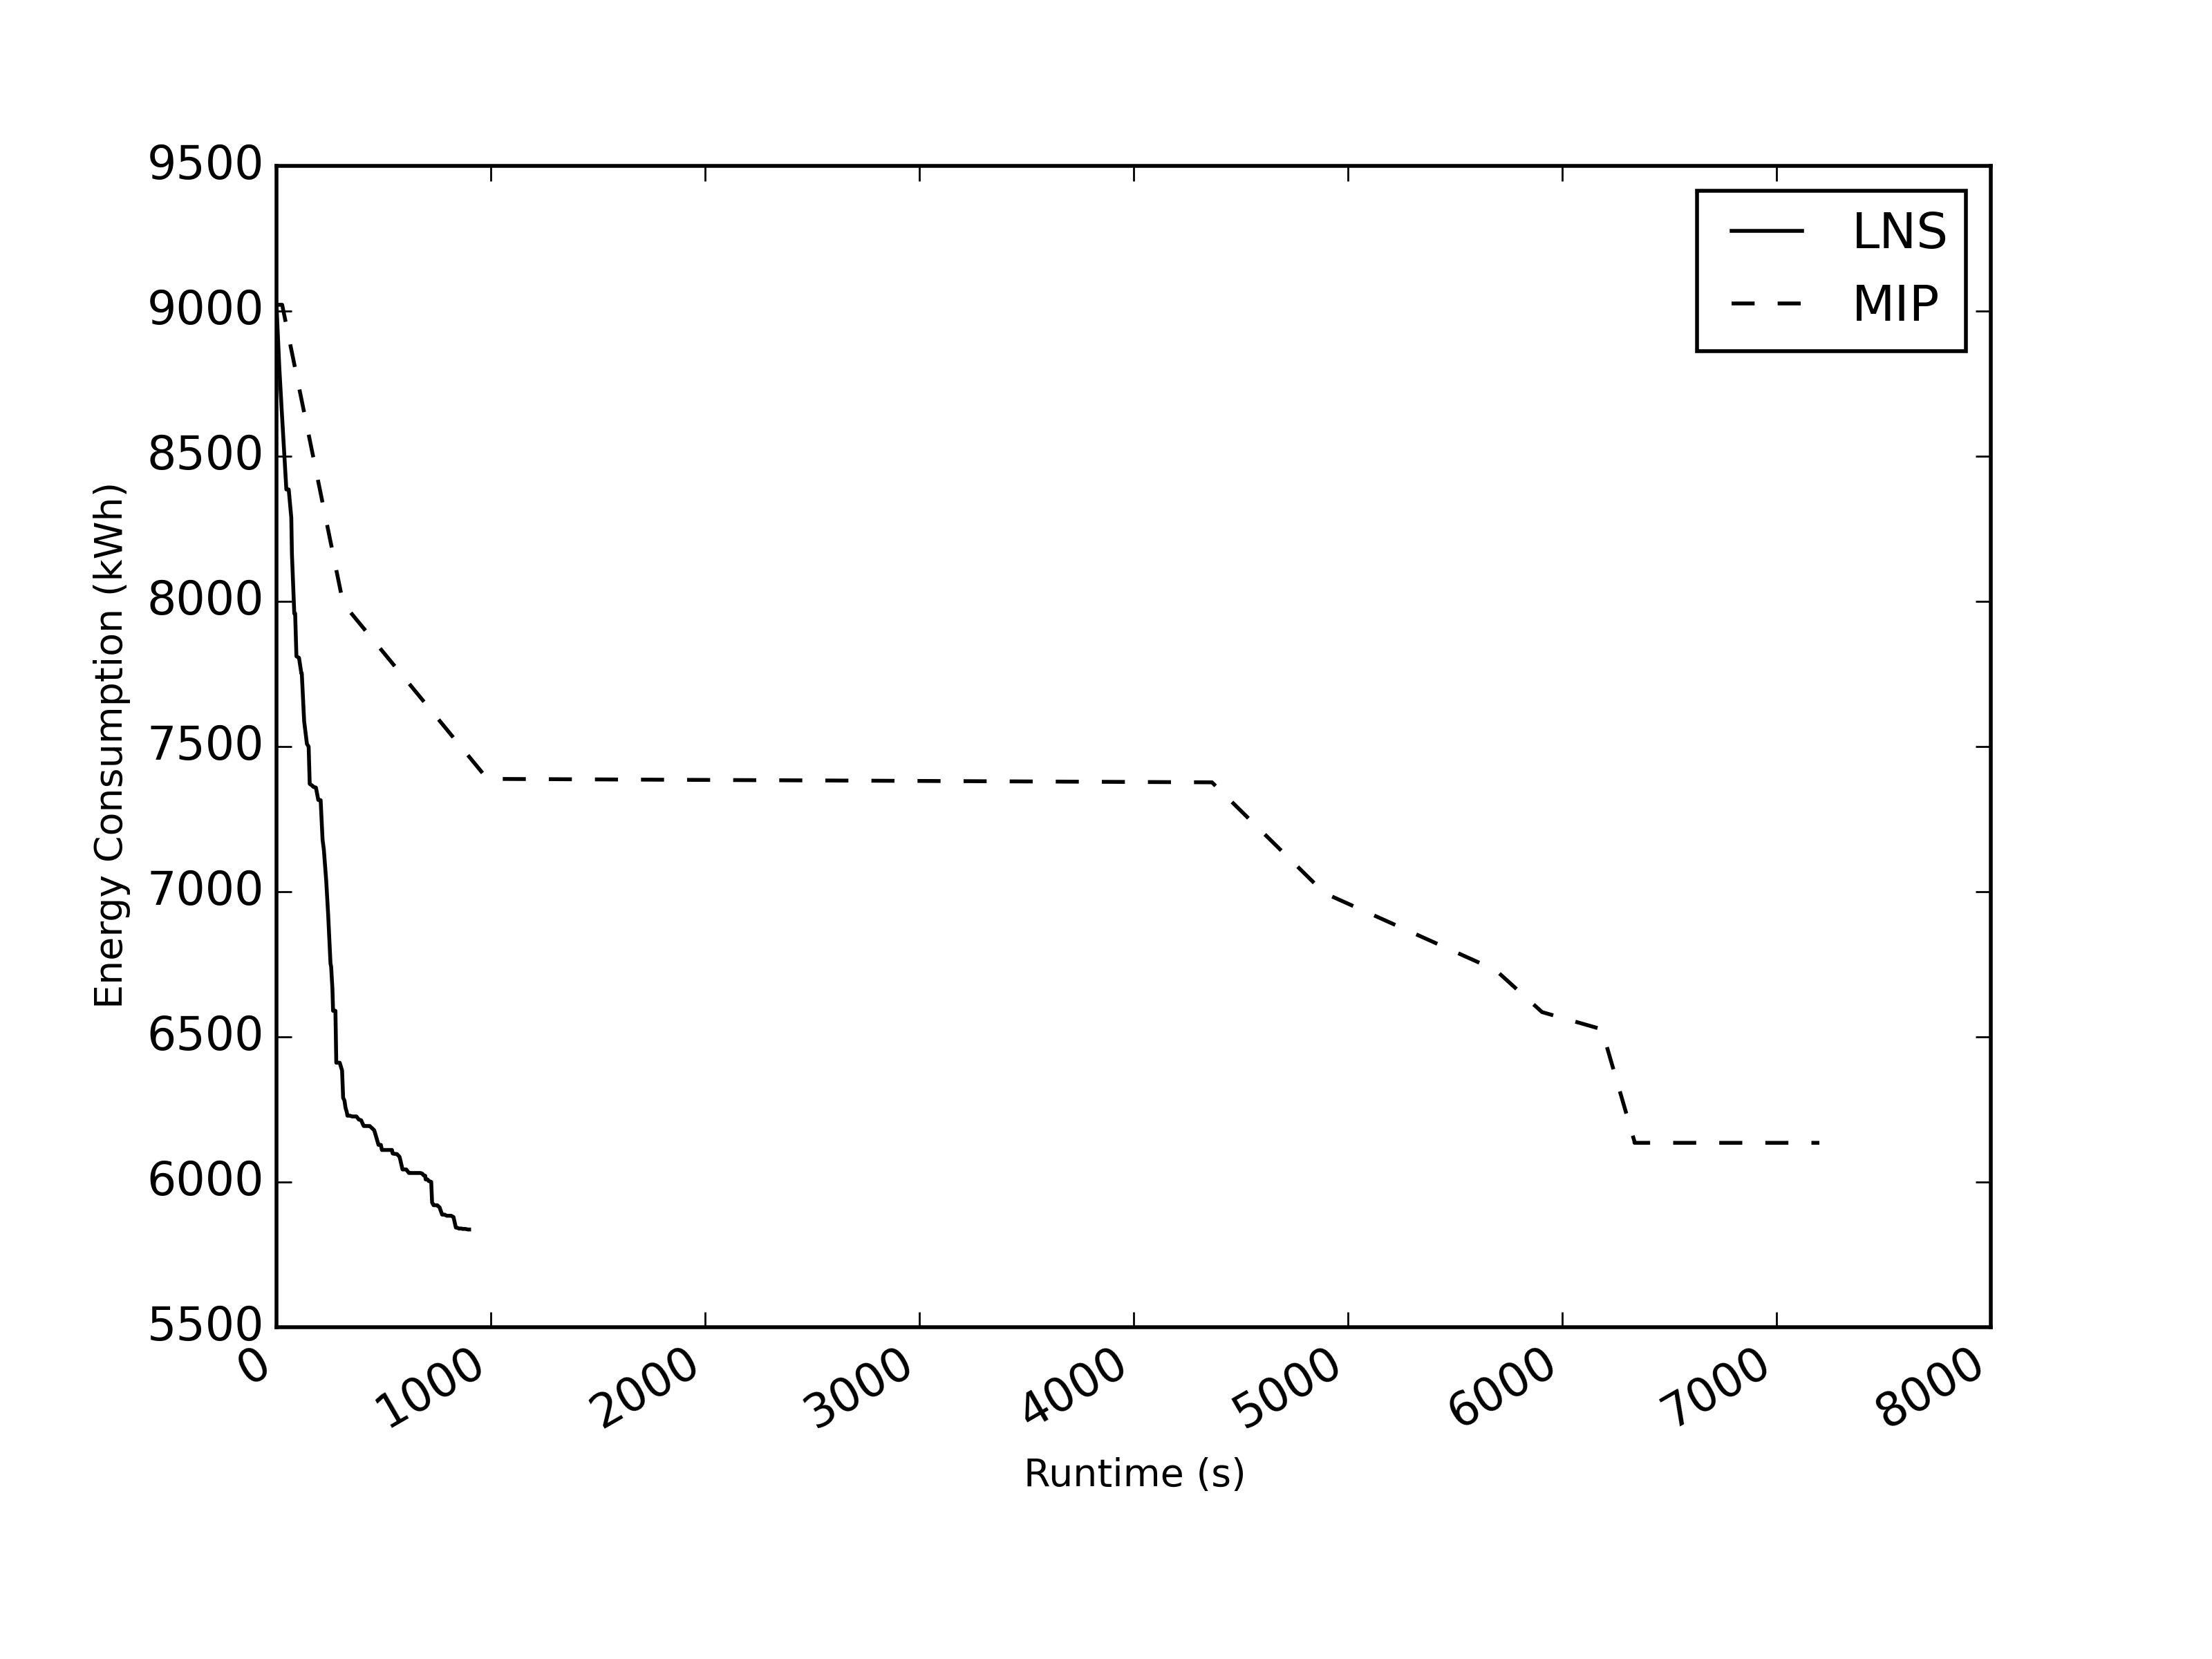
\includegraphics[width=0.9\linewidth]{figs/eams_meeting_m200_2.png} \\
(a) Instance 1  \\[6pt]
		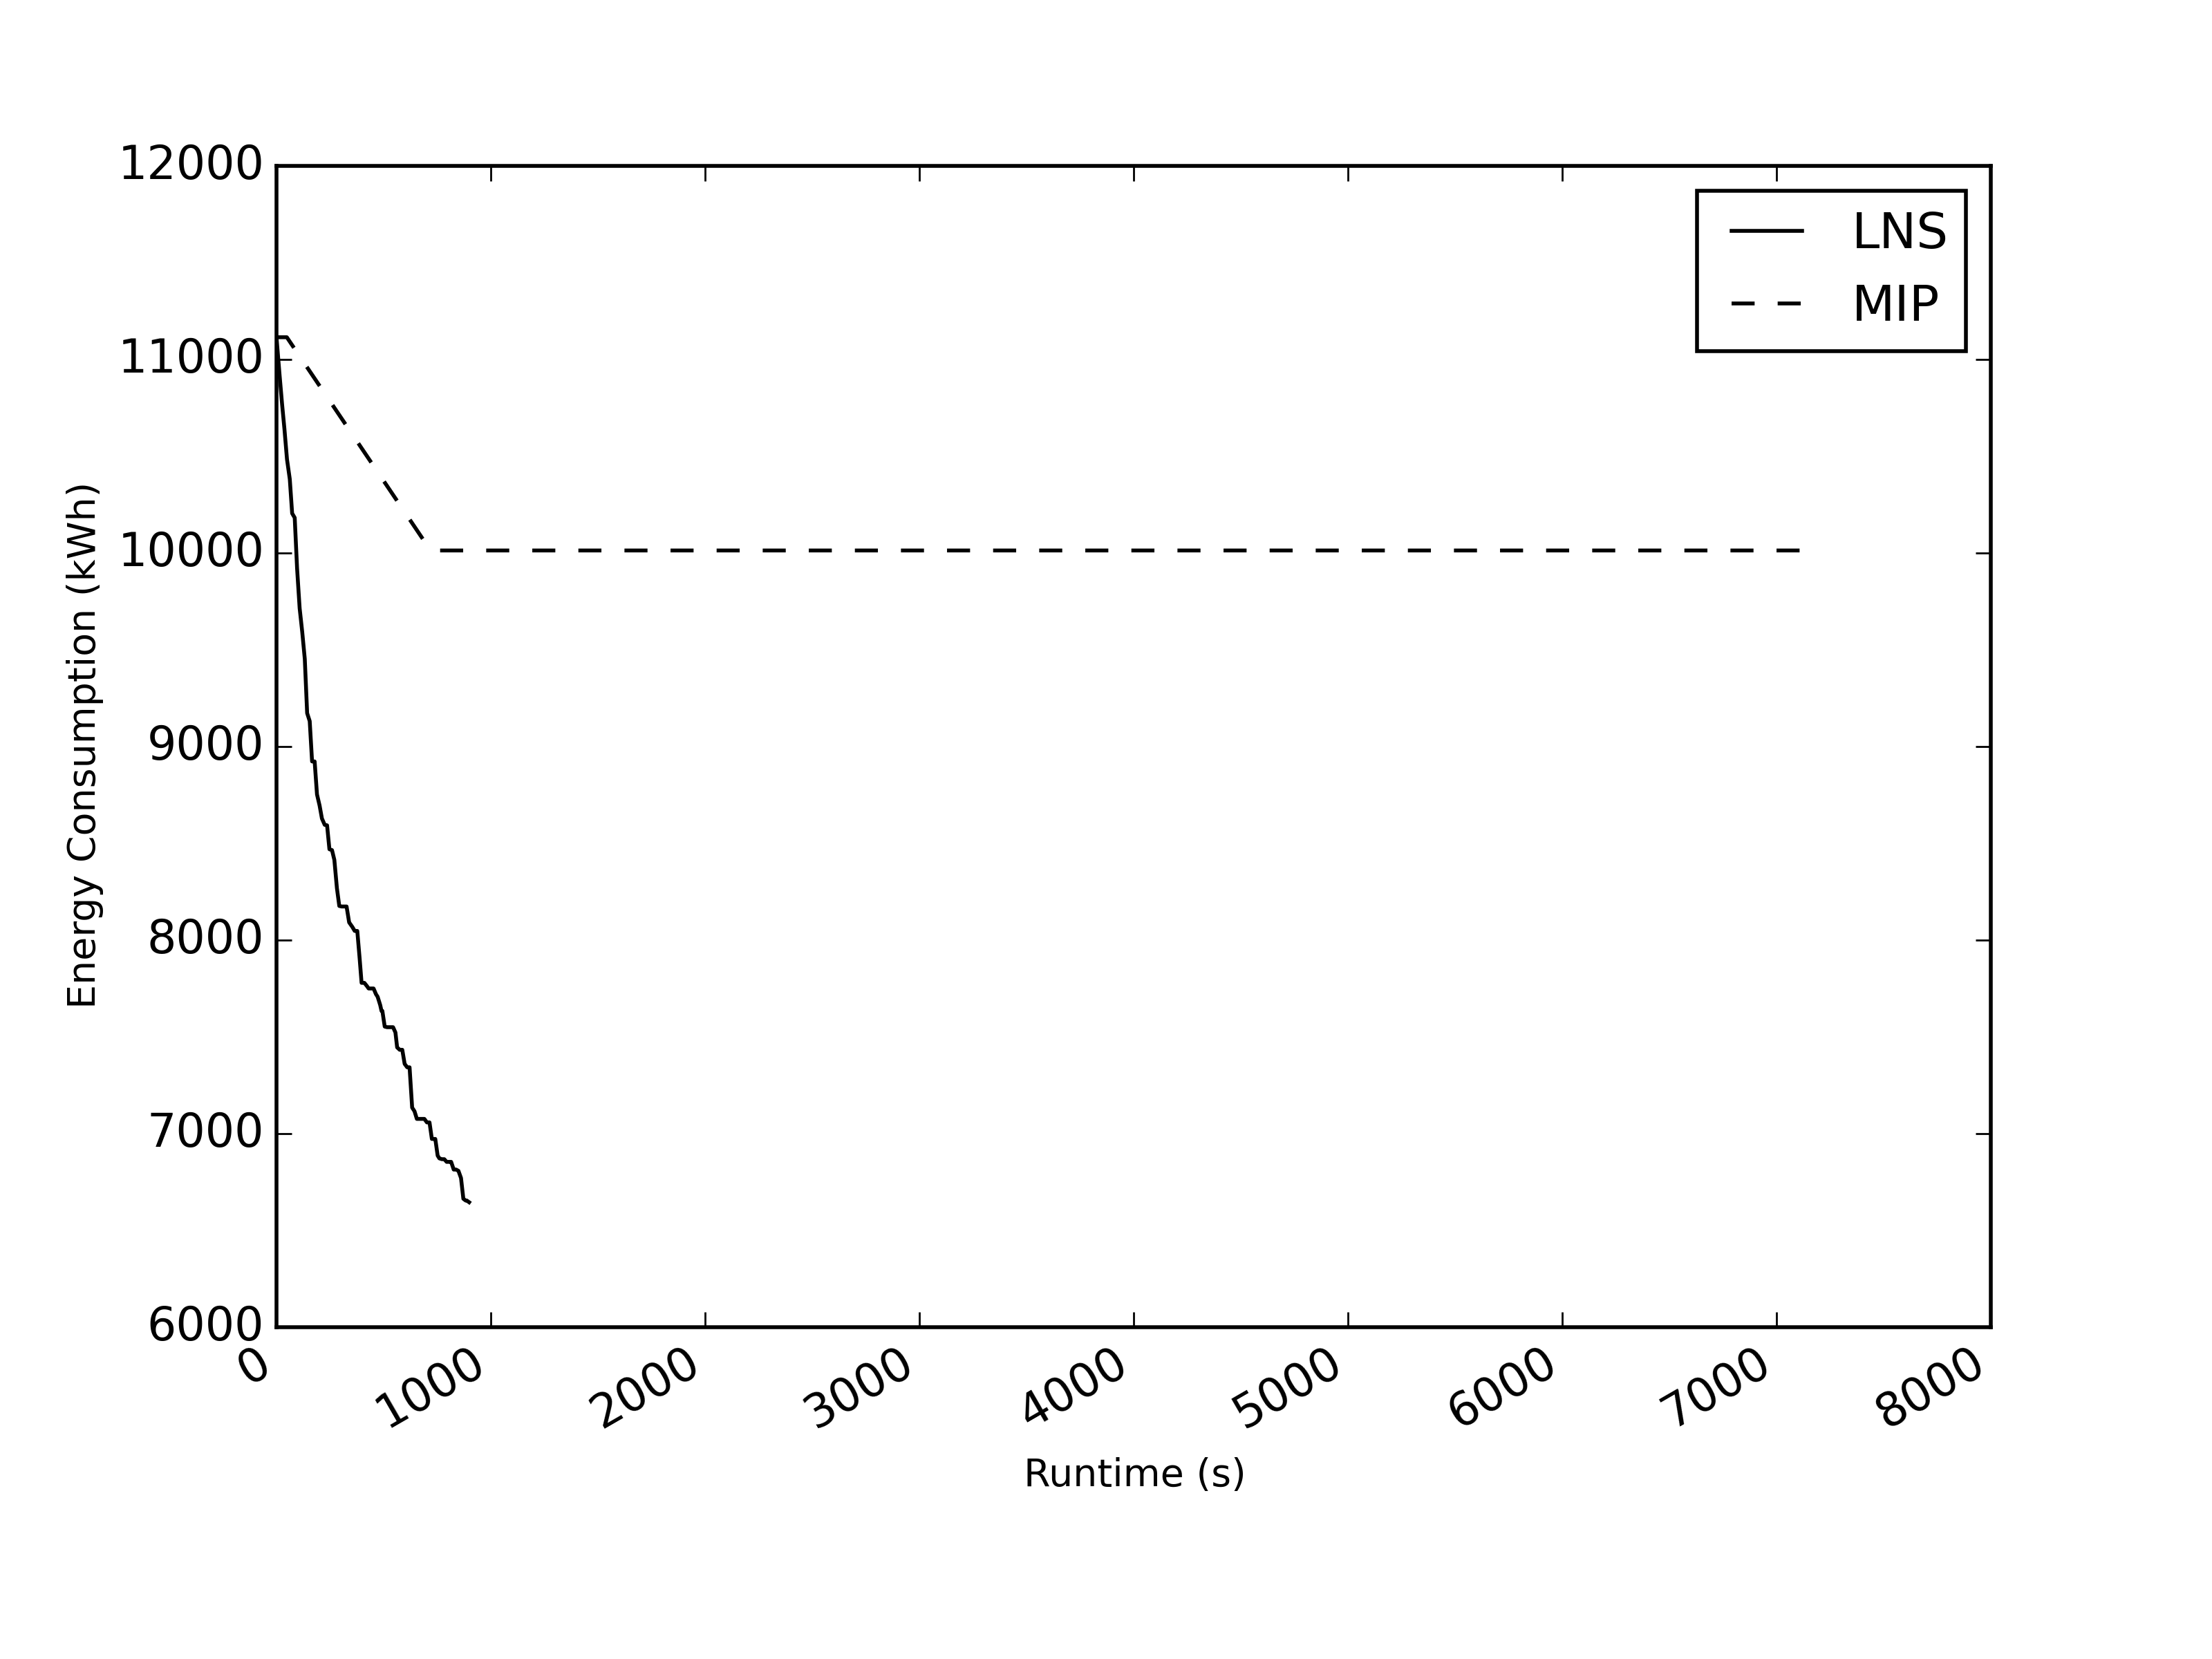
\includegraphics[width=0.9\linewidth]{figs/eams_meeting_m200_1.png}\\
(b) Instance 2  \\[6pt]
	\caption{Typical performance of MIP (2 hours) and LNS (15 minutes) on two benchmark instances.}
	\label{fig:compare}
\end{figure}

Before describing our main results, we first point out the typical behavior of solving energy aware meeting scheduling as a MIP. Figure \ref{fig:compare} shows the performance of the MIP approach on two typical problem instances when given 2 hours of runtime. In general, MIP's convergence on large problems is slow and sometimes MIP fails to converge even after 2 hours. This is exactly why we developed the LNS approach. The typical performance of the LNS approach is also given in Figure \ref{fig:compare}. In the figure, LNS was given only 15 minutes of runtime but it is capable of returning significantly better results when compared to MIP.



\subsection{Combining MIP with LNS}\label{sec:lns_eg}

\begin{figure}
	\centering
		\includegraphics[width=0.9\linewidth]{figs/lns_sche_init1.jpg} \\
(a) Initial schedule  \\[6pt]
		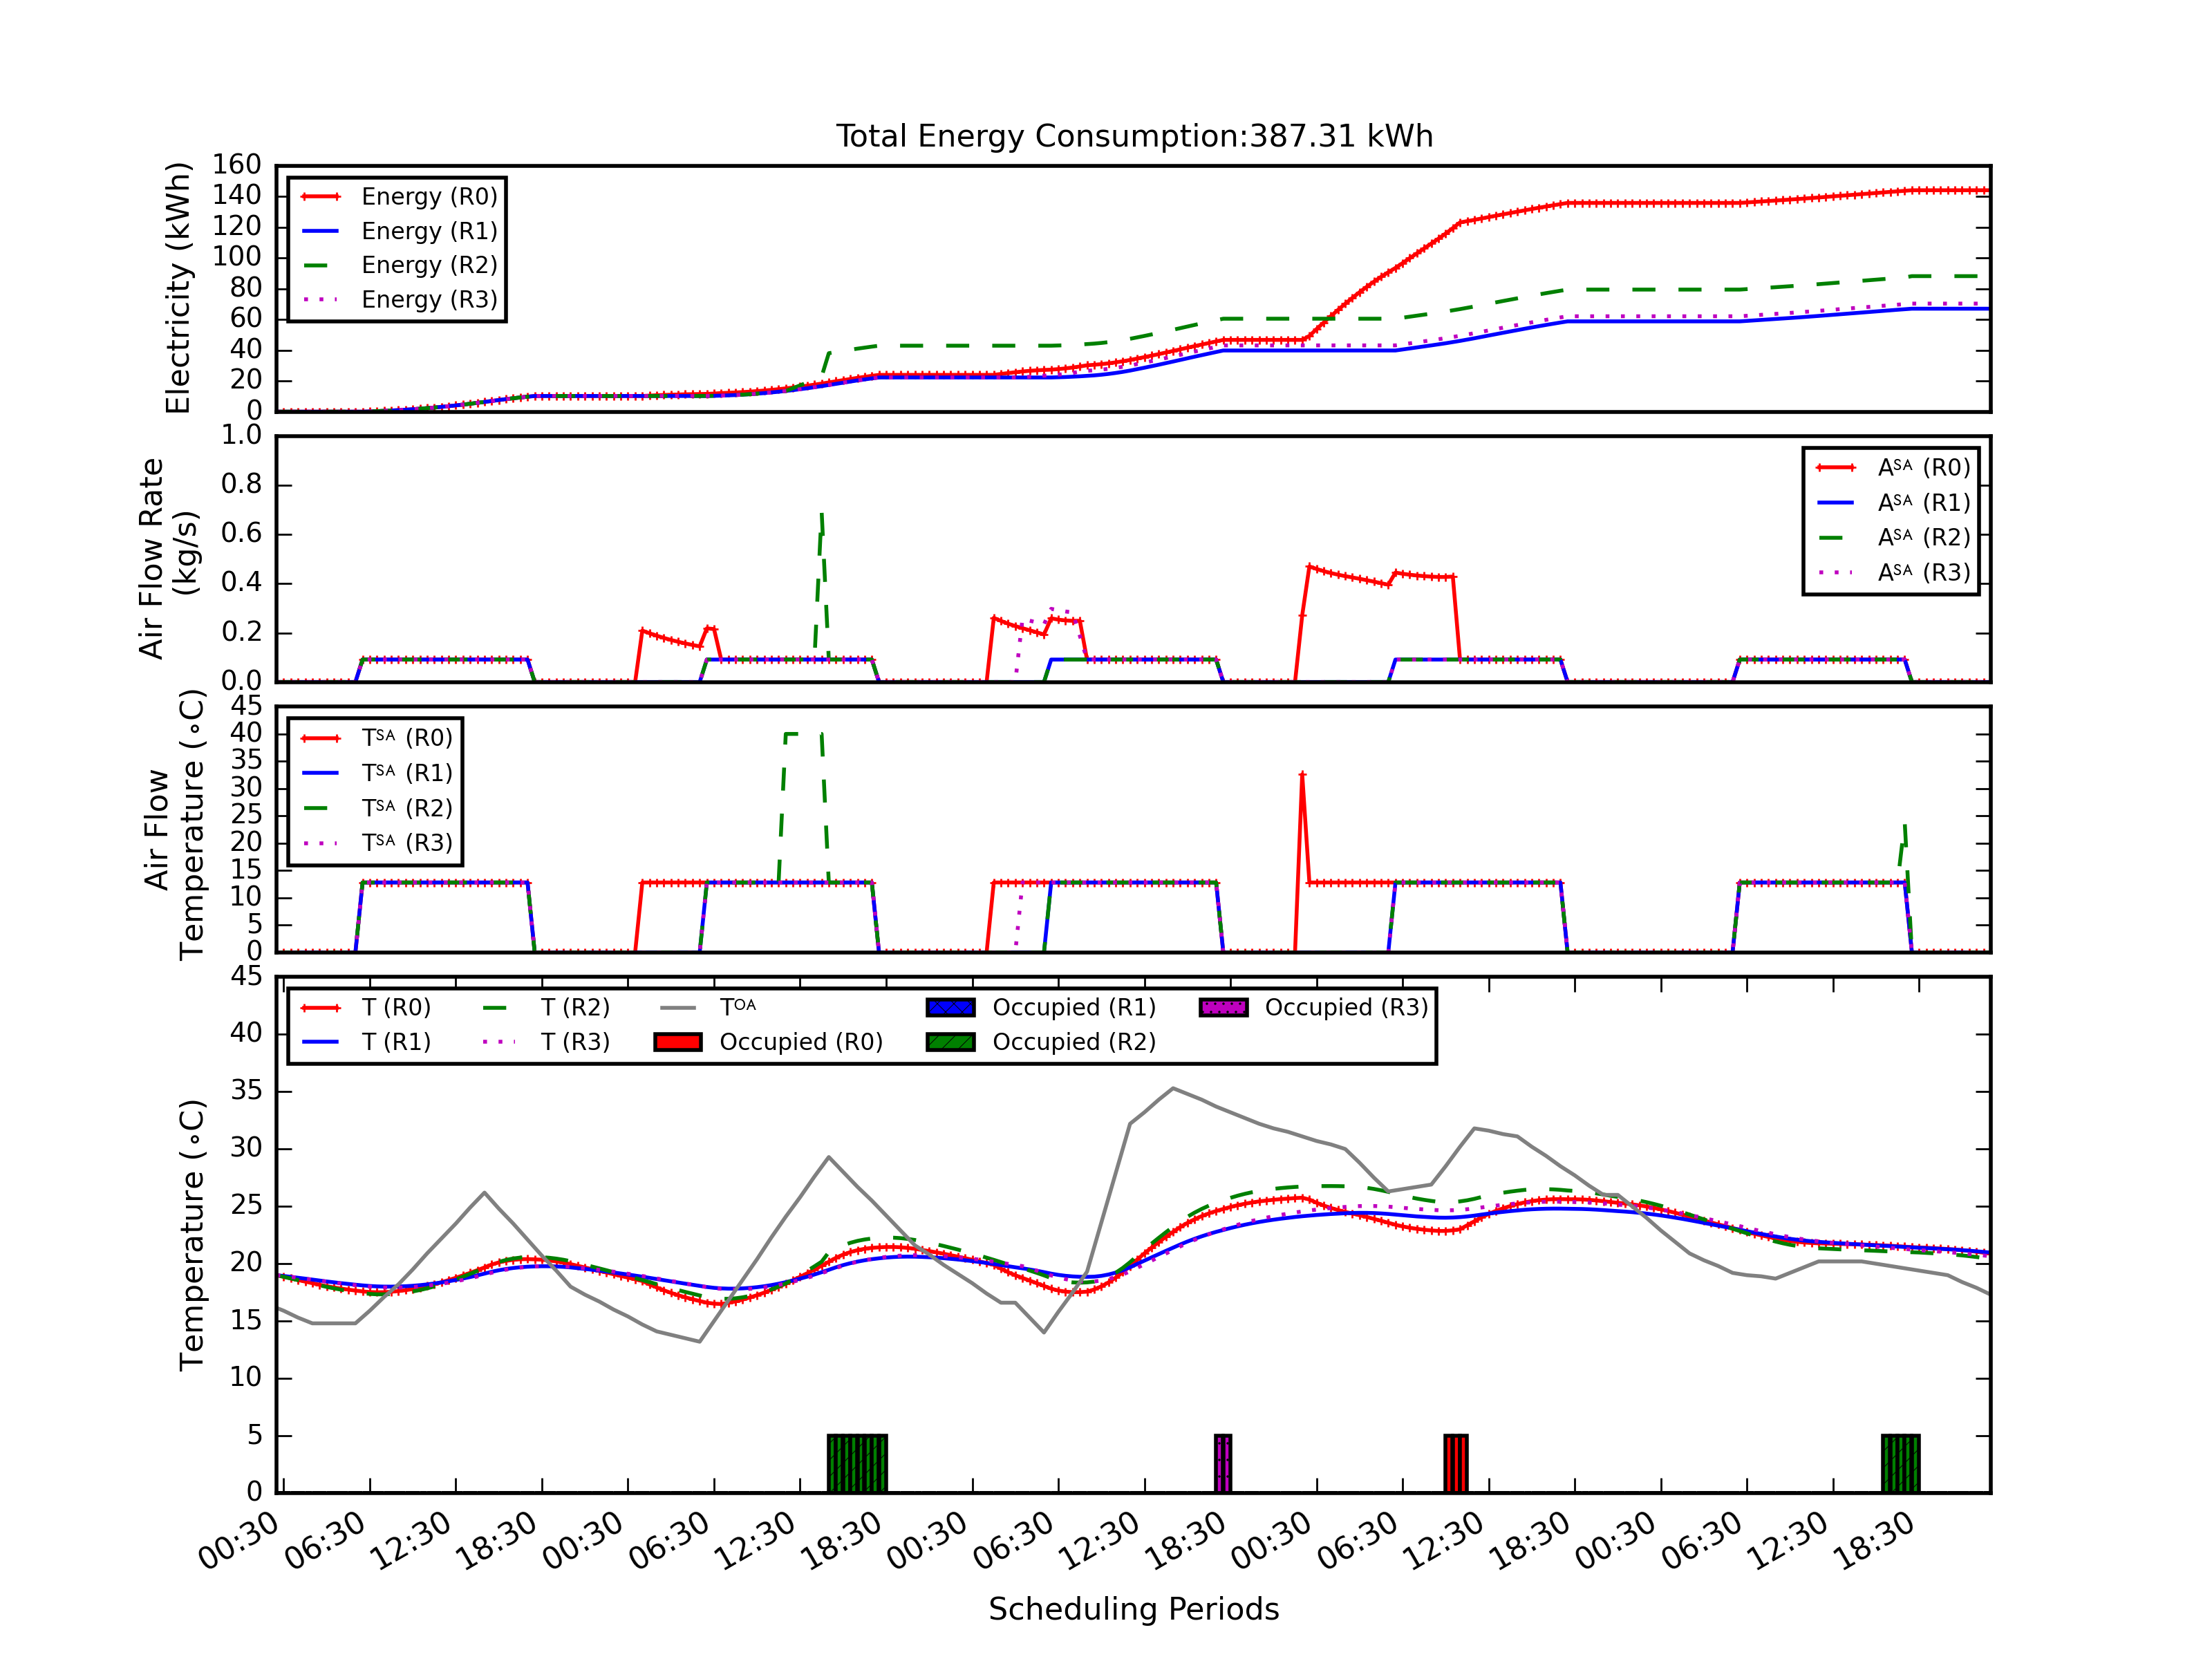
\includegraphics[width=1\linewidth]{figs/lns_init.png}\\
(b) HVAC control for Room R0-R3  \\[6pt]
	\caption{Large neighbourood search - initial schedule}
	\label{fig:lns_init}
\end{figure}

Figure \ref{fig:lns_init}--\ref{fig:lns_dr3} illustrate a high-level scenario example of our large neighbourhood search approach. These figures give an insight of how schedules are being initialized, destroyed and repaired over 5-days in 20 rooms using our LNS algorithm. In Figure \ref{fig:lns_init}(a), an initial schedule is generated by greedily scheduling all meetings in the minimum number of rooms each day. More rooms are used only if there are overlapping meetings that have to be scheduled in different locations. This schedule is then fed into our occupancy-based HVAC control model. Figure \ref{fig:lns_init}(b) shows the optimised HVAC control based on the given schedule. With this initialization approach, we can quickly generate an initial feasible schedule and an optimal HVAC control for large number of meetings and rooms. For simplicity, only the HVAC controls for room R0 to R3 are shown. Note that 1 slot in \ref{fig:lns_init}(a) is equivalent to 2 slots in \ref{fig:lns_init}(b), and the occupied slots are depicted as vertical blocks (30 minutes each) in the third subgraph of \ref{fig:lns_init}(b). 
% Standby mode is on, hence wwe see that the HVAc is activated in R0 and R3 during off peak hour to pre-cool the rooms.
% R2 is warmed up with high TSA.


\begin{figure}
	\centering
		\includegraphics[width=0.9\linewidth]{figs/lns_sche_ds1.jpg} \\
(a) Schedule: destroy \& repair room R0 and room R1 \\[6pt]		
		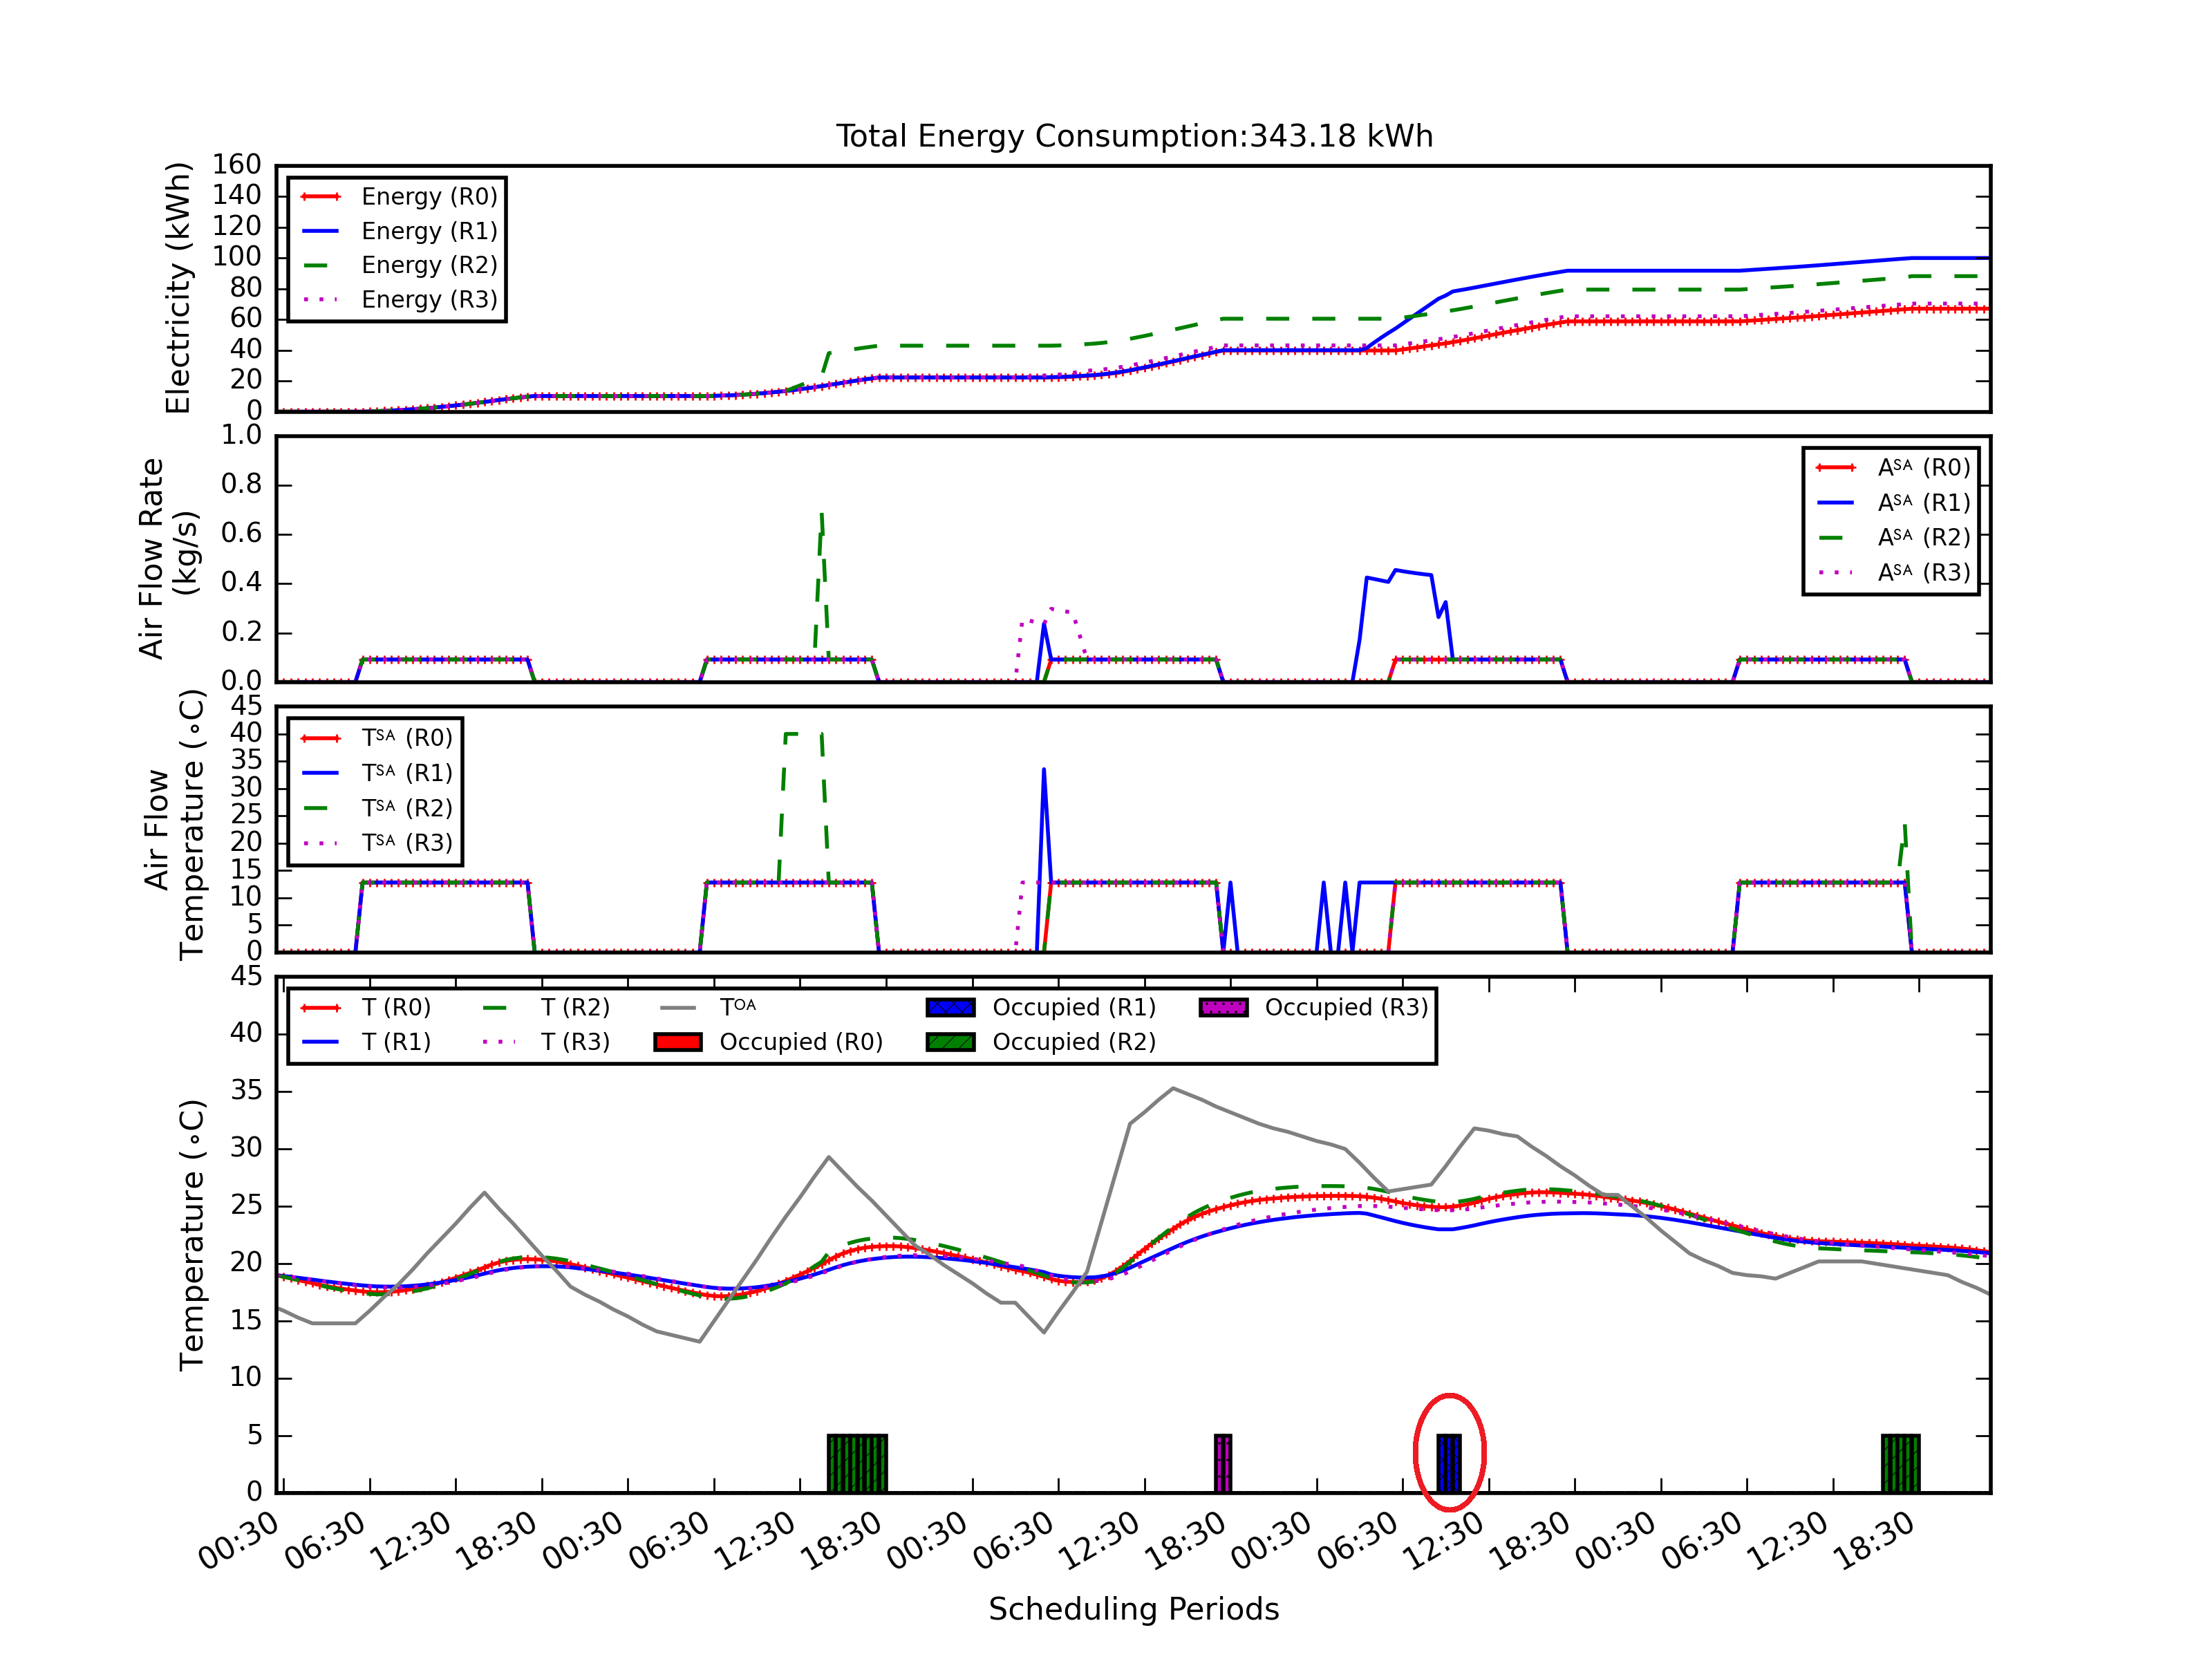
\includegraphics[width=1\linewidth]{figs/lns_dr1.png} \\
(b) HVAC control for Room R0-R3  \\[6pt]
	\caption{Large neighbourood search - iteration 1: destroy \& repair steps}
	\label{fig:lns_dr1}
\end{figure}

Figure \ref{fig:lns_dr1} depicts the first iteration of the destroy and repair step. In this iteration, Room R0 and Room R1 are randomly selected. All meetings scheduled in Room R0 and Room R1 are destroyed, and a schedule re-optimisation is executed. In this scenario, meetings in Room R0 are moved to Room R1, as shown in Figure \ref{fig:lns_dr1}(a). We observe from Figure \ref{fig:lns_dr1}(b) that this leads to a reduction of 44 kWh. %We observe from Figure \ref{fig:lns_dr1}(b) that this occurs as an energy reduction of 44 kWh can be achieved by simply swapping the meetings from room R0 to room R1.


\begin{figure}
	\centering
		\includegraphics[width=0.9\linewidth]{figs/lns_sche_ds2.jpg}\\
(a) Schedule: destroy \& repair room R0 and room R3  \\[6pt]
		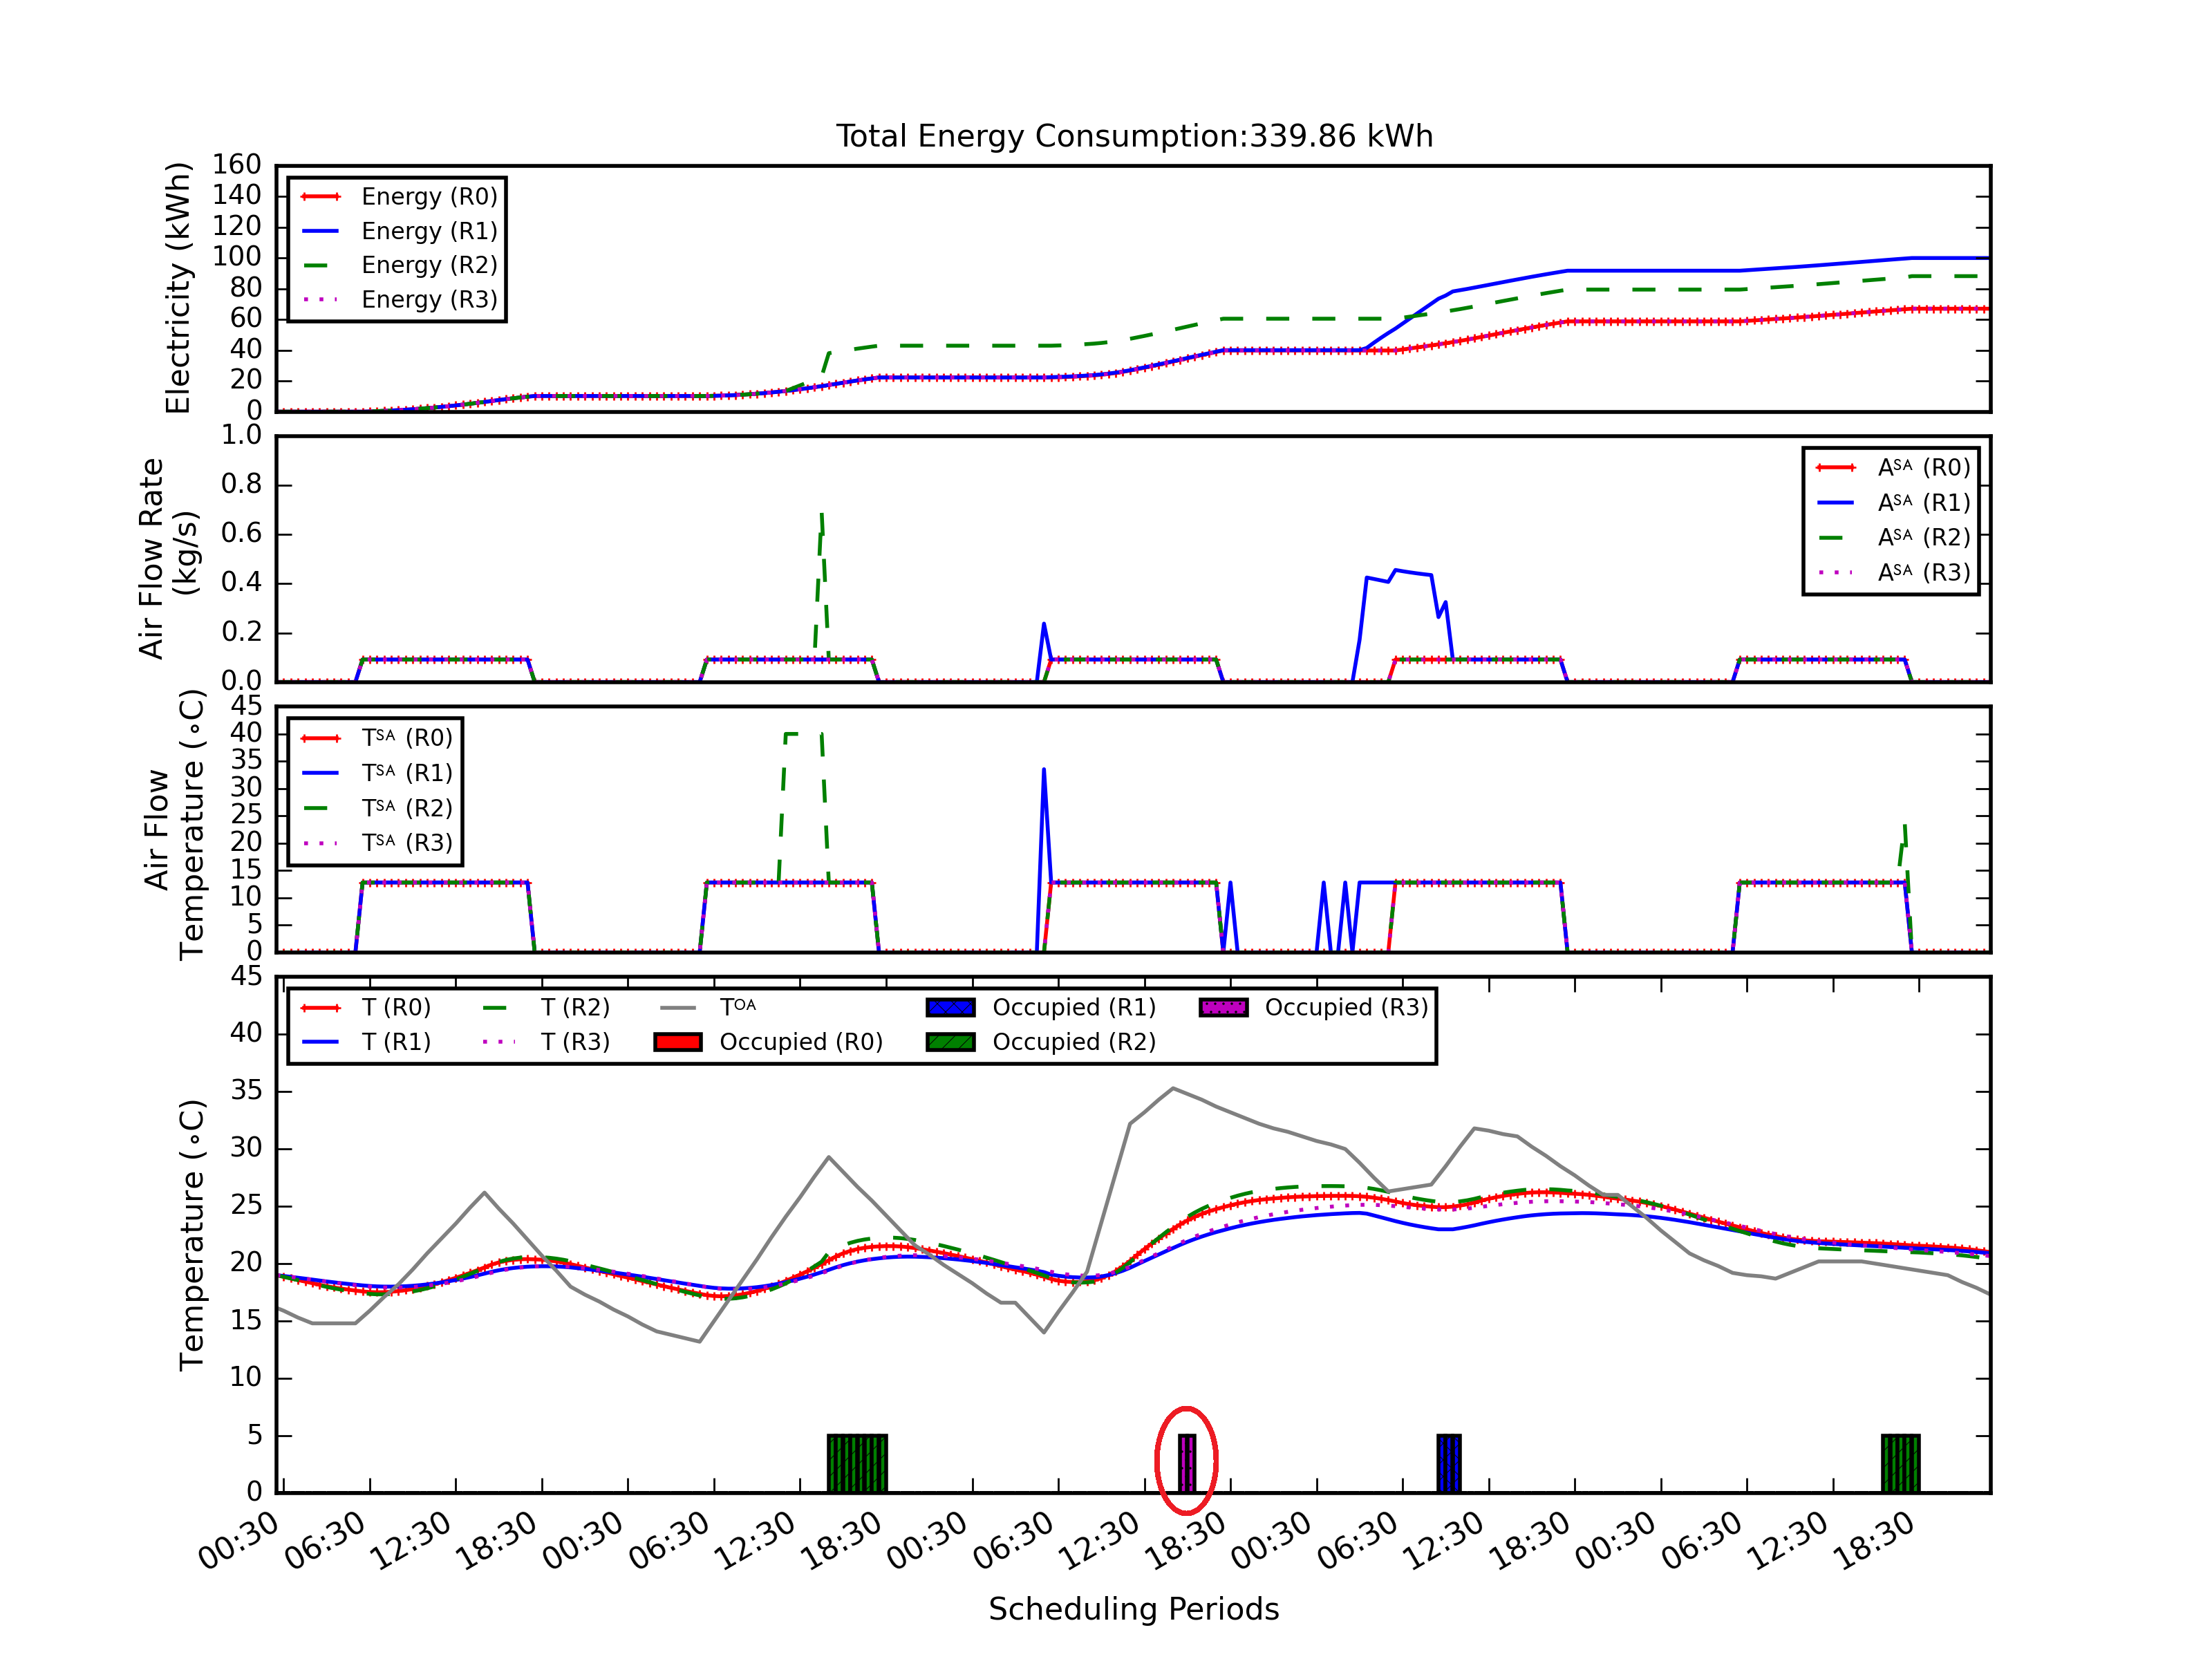
\includegraphics[width=1\linewidth]{figs/lns_dr2.png} \\
(b) HVAC control for Room R0-R3  \\[6pt]
	\caption{Large neighbourood search - iteration 2: destroy \& repair steps}
	\label{fig:lns_dr2}
\end{figure}

Figure \ref{fig:lns_dr2} presents the second iteration of destroy and repair step. In this round, Room R0 and Room R3 are selected. There is no meeting scheduled in R0 now. However, a better schedule is found by re-scheduling meetings in Room R3 to earlier time slots, as shown in Figure \ref{fig:lns_dr2}(a). Figure \ref{fig:lns_dr2}(b) reveals the reason behind this move. By moving the meetings 2.5 hours earlier, it helps to reduce the supply air flow rate required to maintain the room temperature at comfort bounds, as that day has relative high outdoor temperature. By doing this, a 3.32kWh of energy is saved.


\begin{figure}
	\centering
		\includegraphics[width=0.9\linewidth]{figs/lns_sche_ds3.jpg}\\
(a) Schedule: destroy \& repair room R0 and room R2  \\[6pt]
		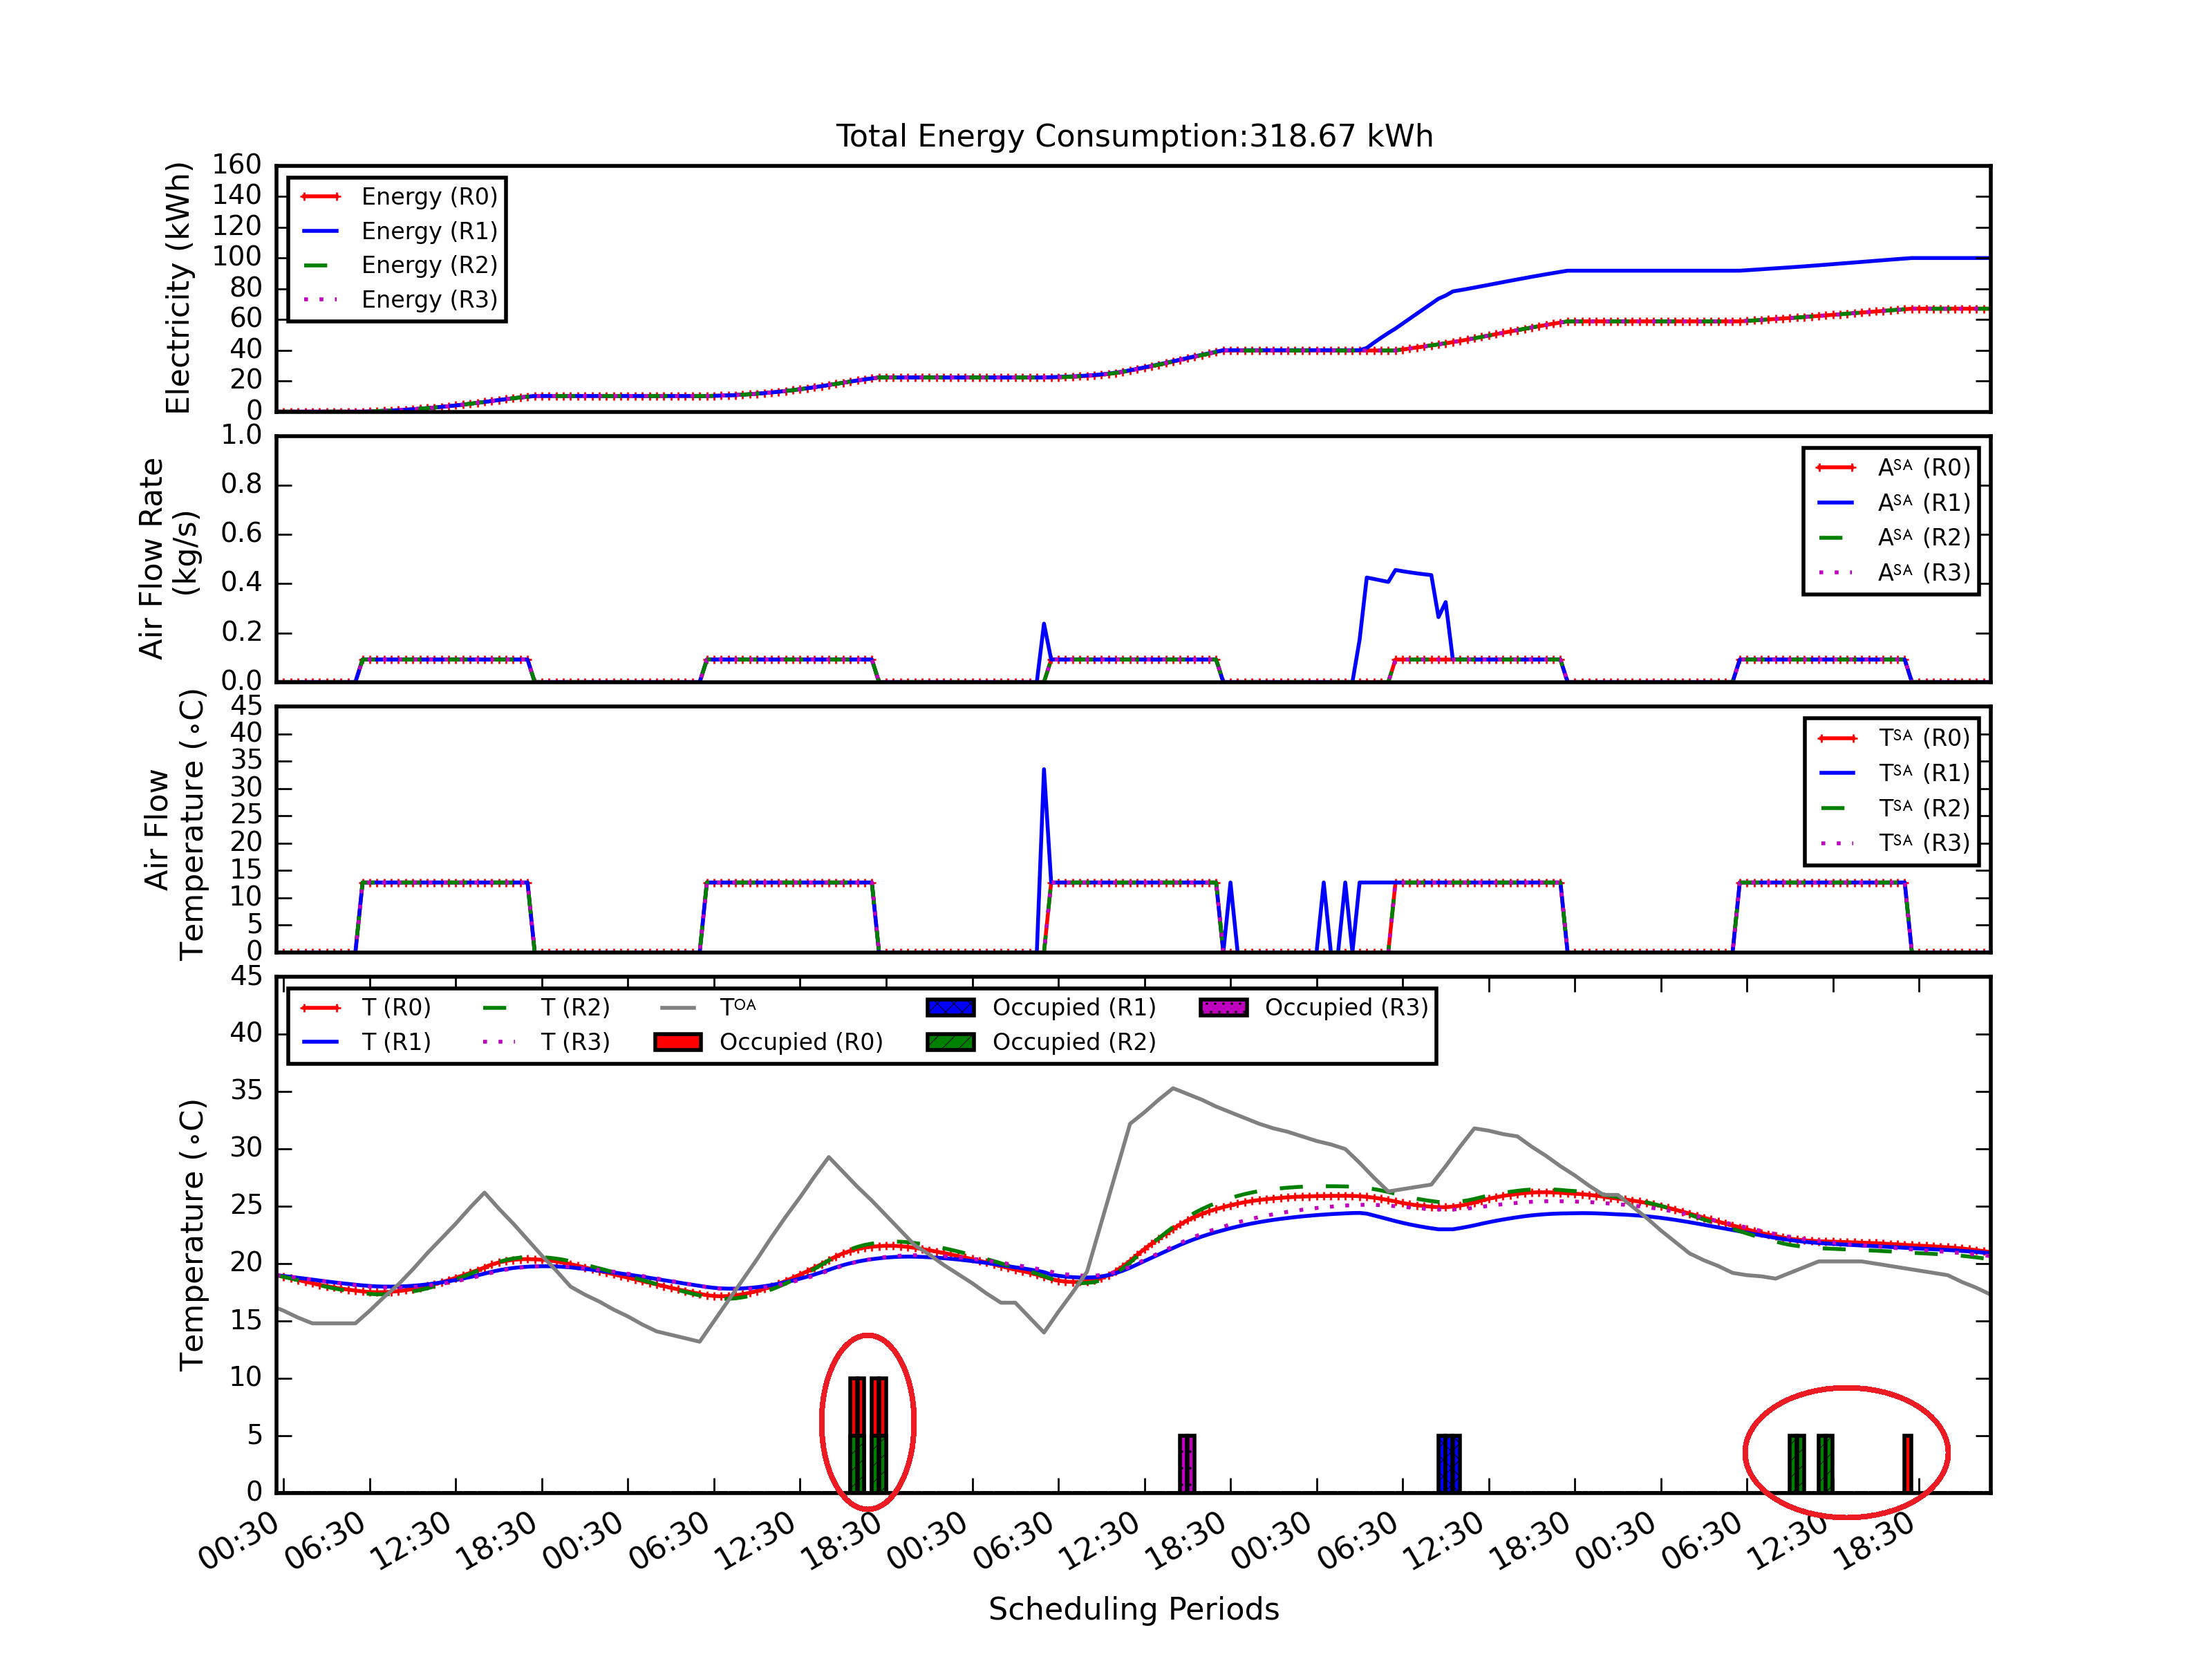
\includegraphics[width=1\linewidth]{figs/lns_dr3.png} \\
(b) HVAC control for Room R0-R3  \\[6pt]
	\caption{Large neighbourood search - iteration 3: destroy \& repair steps}
	\label{fig:lns_dr3}
\end{figure}

During the third iteration of the destroy and repair step, room R2 and R0 are selected. Figure \ref{fig:lns_dr3}(a) shows that an improvement is made on the schedule by moving some meetings in Room R2 to Room R0 and relocating another meeting to a different time slot in Room R2. As depicted in Figure \ref{fig:lns_dr3}(b), if meetings are held in parallel, minimum supply air flow rate is required to achieve the occupied thermal comfort temperature in both room R0 and R2. The same happens if meetings are moved to earlier time of the day in room R2 or re-located to room R0 on the fifth day of the scheduling period. With this improvisation, an additional 21.19kWh is conserved.

In conclusion, this example shows that by combining LNS and MIP, our joint model achieves a reduction of 68 kWh within 3 destroy and repair rounds. Each iteration of destroy and repair takes only 10 seconds.  Given a relative small number of rooms, our MIP model is capable of finding an optimal solution\footnote{a locally optimal solution within the sub-space specified by the destroy step}, within a short period of time. 


\subsection{Large-scale Experiments}

We analyze our LNS approach by considering 8 problem sets. Each problem set contains 10 problem instances that we built by adding energy related information to instances extracted from the PATAT timetabling dataset \citep{patat02}. The problem sets differ by the number of meetings (M) and the number of rooms (R). Specifically, our problem sets are referred to as 20M-20R, 50M-20R, 100M-20R, 200M-20R, 50M-50R, 100M-50R, 200M-50R, and 500M-50R, where 20M-20R represents the problem set with 20 meetings and 20 rooms. All our experiments were run on a cluster that consists of a 2 $\times$ AMD 6-Core Opteron 4334, 3.1GHz with 64GB memory.

In each problem set we must schedule up to 500 meetings whose durations are 1 or 1.5 hours. The meetings must be scheduled over a period of 5 summer days. All meetings have between 2 and 30 attendees and we vary the scheduling flexibility for each meeting with an allowable time range of one or two random days (between 09:00-17:00) within the 5 summer days. 
We adopt similar buildings' zone layout and configurations as defined in Section \ref{sec:mip:experiments}. 
The available rooms are located in 5 buildings, that differ by their thermal resistance and capacitance as specified in Table \ref{tab:rc_wall_win}. We use a $1\times4$ zone layout where each zone has the same thermal resistance and capacitance as its neighboring zones. Moreover, all rooms have the same geometric area of $6\times10\times3$ m$^3$ with a window surface area of $4\times2$ m$^2$ and a capacity of 30 people. The solar gain ranges from $50$ to $350$~W/m$^2$ during the day. 

\begin{figure}
	\centering
		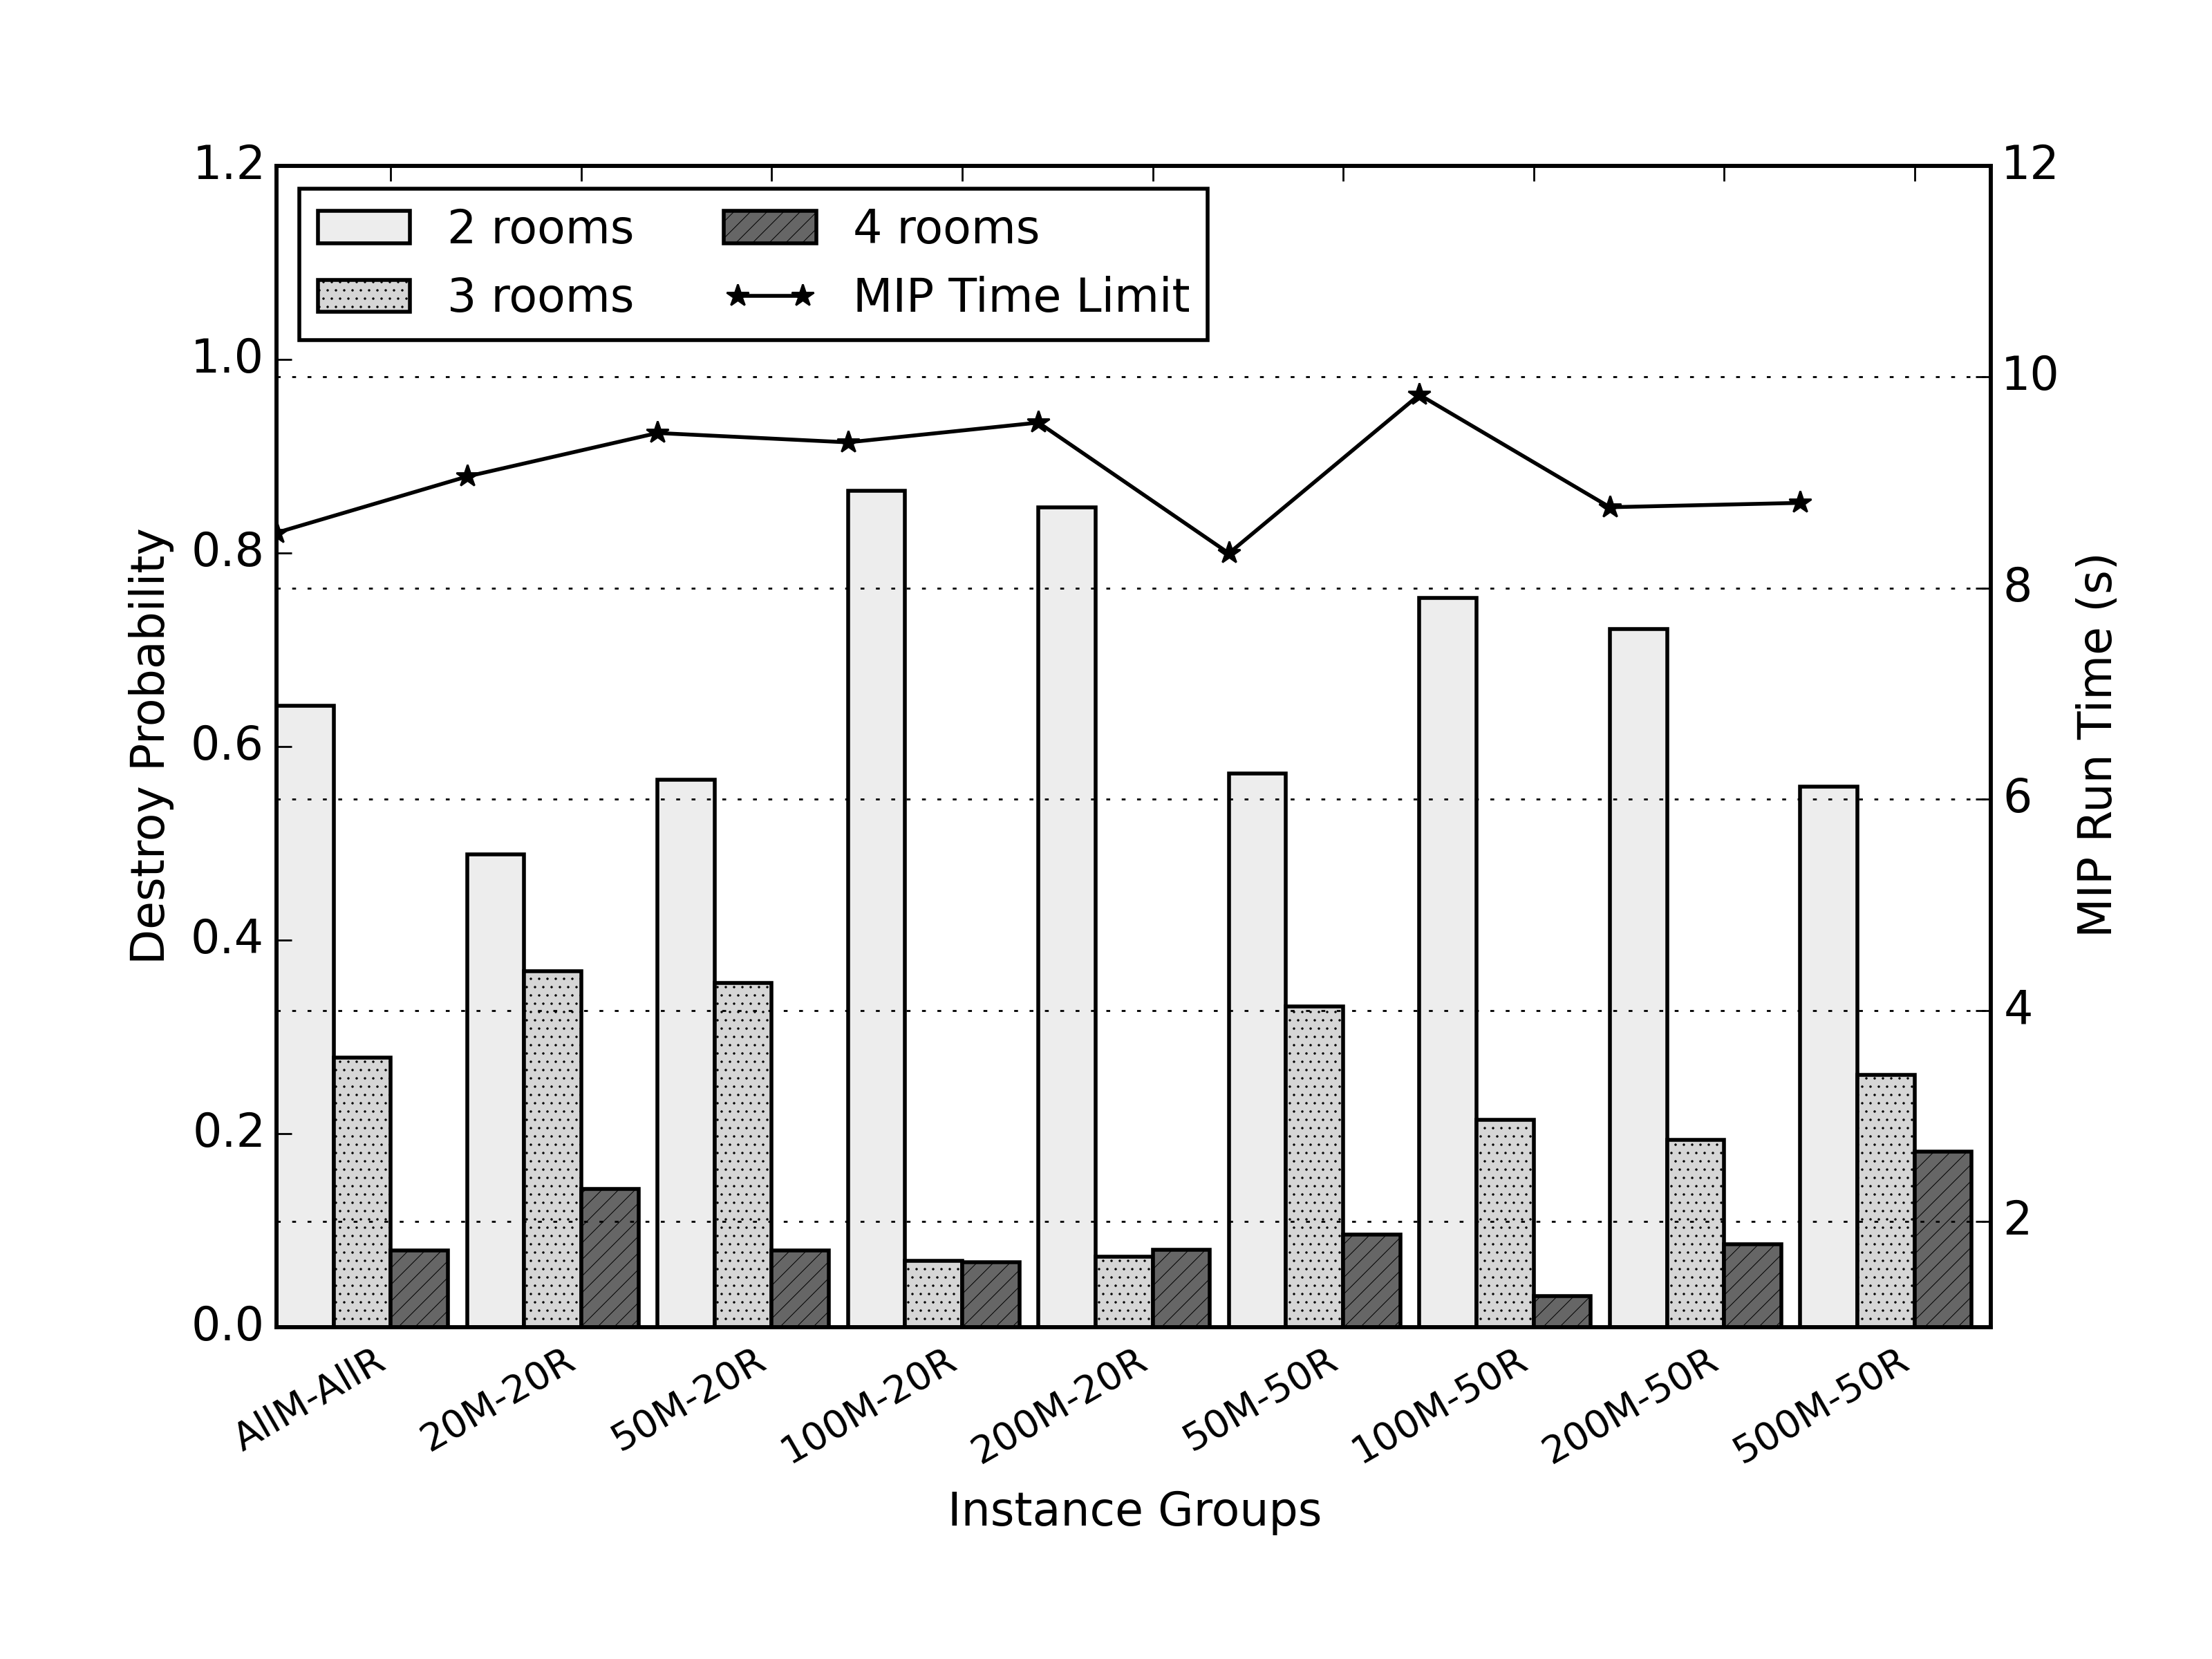
\includegraphics[width=0.9\linewidth]{figs/mipdestroy_1027.png}
	\caption{Parameter configurations as determined by SMAC.}
	\vspace*{-2ex}
	\label{fig:mipdestroy_0907}
\end{figure}

\begin{figure}
\centering	
	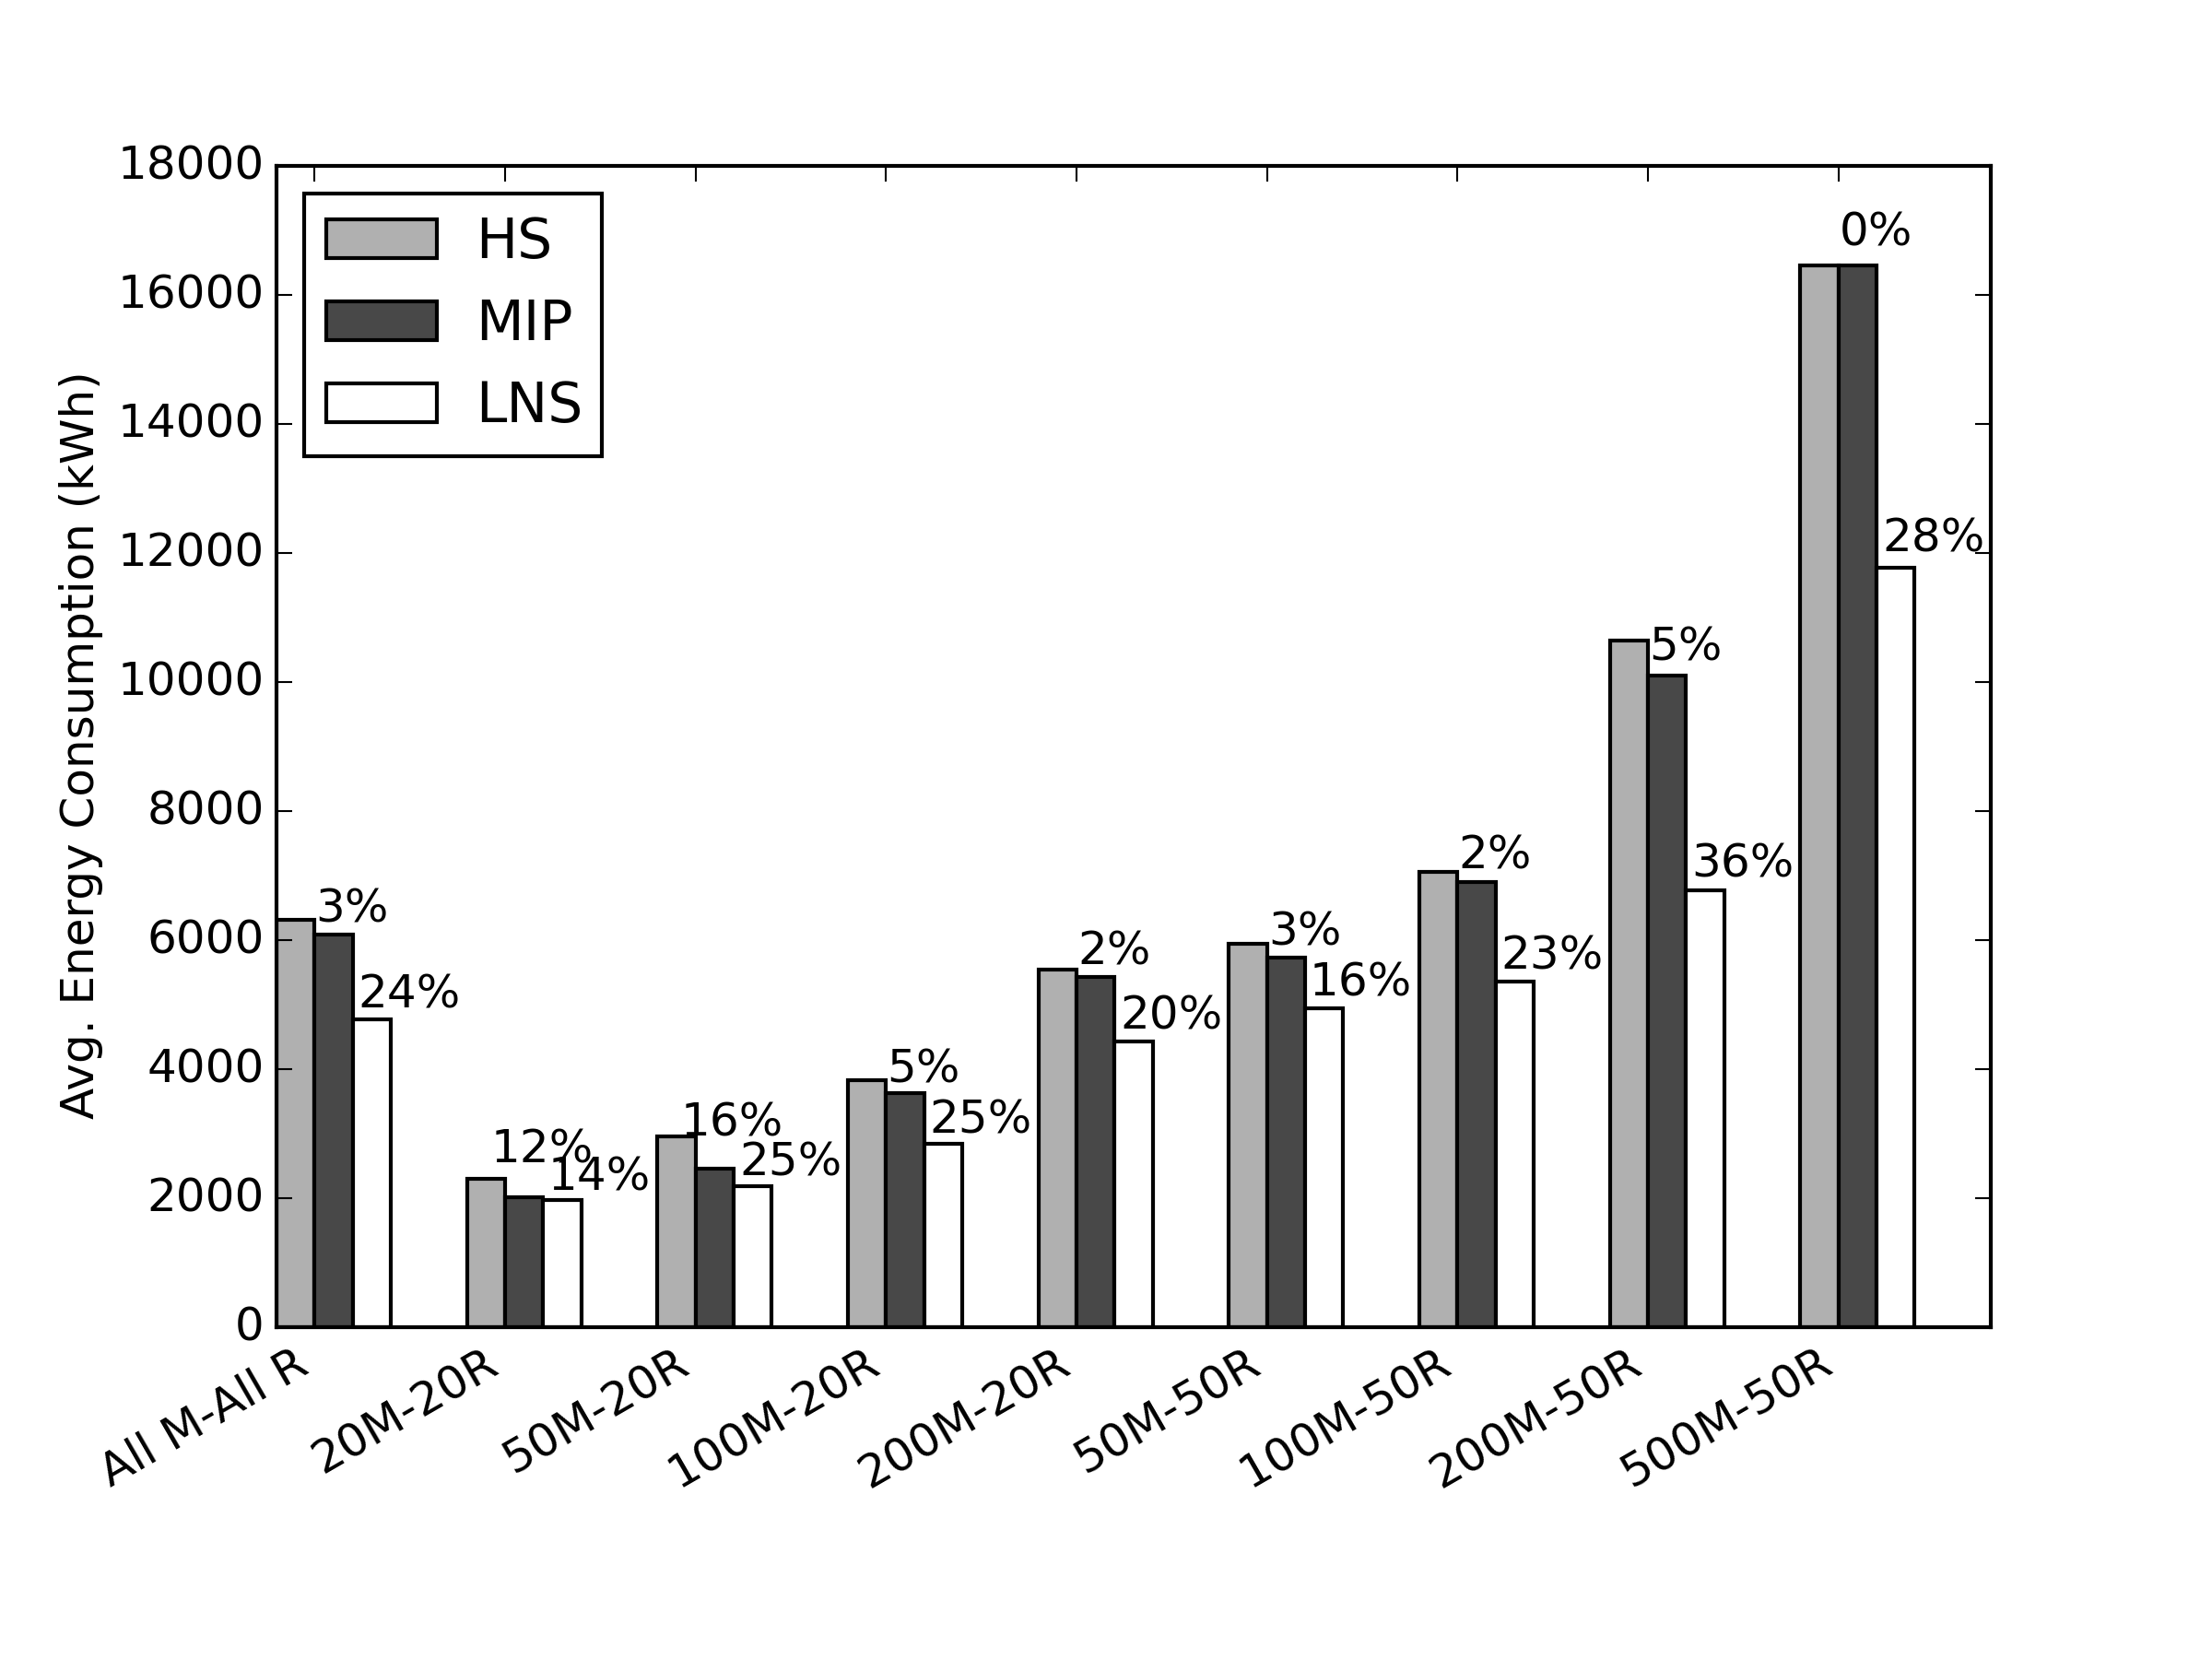
\includegraphics[width=0.9\linewidth]{figs/lnsmip_mspec_mspec900_shortHS_maxdata500.png}
	\caption{Performance improvement of MIP and LNS over heuristic solution (HS). MIP and LNS runtime 15 minutes.}
	\vspace*{-2ex}
\label{fig:mspec_mspec_900}
\end{figure}

First, we used SMAC to tune the parameters for all 80 instances. %It is, however, possible that the parameters of the LNS may have an impact on the performance of LNS when solving a problem instance.
However, it is possible that one set of parameter configurations might not produce best results across all problem sets.
For example, \cite{malitsky2013tuning} observed that instance specific algorithm configuration finds good quality solutions for large sized instances in limited time. Hence, second we independently tuned the parameters for the 8 problem sets. In each case, we used 0.33, 0.33, and 0.34 as the default destroy probabilities and 5 seconds for the default MIP runtime during each repair step. SMAC trains on 60\% of the instances and cross-validates with the remaining 40\%.

On average, SMAC generated 300 configurations for each problem set. Figure \ref{fig:mipdestroy_0907} shows the best parameter configurations as determined by SMAC for all 80 instances (AllM-AllR), and for the each of the 8 problem sets. In the end, a MIP runtime of 8.5 seconds, and probabilities of 0.64, 0.28, 0.08 to destroy 2, 3, and 4 rooms respectively were determined to be the best settings by SMAC for all 80 instances. However, the best parameter configurations do vary somewhat for the different problem sets.

\begin{figure}
	\centering
		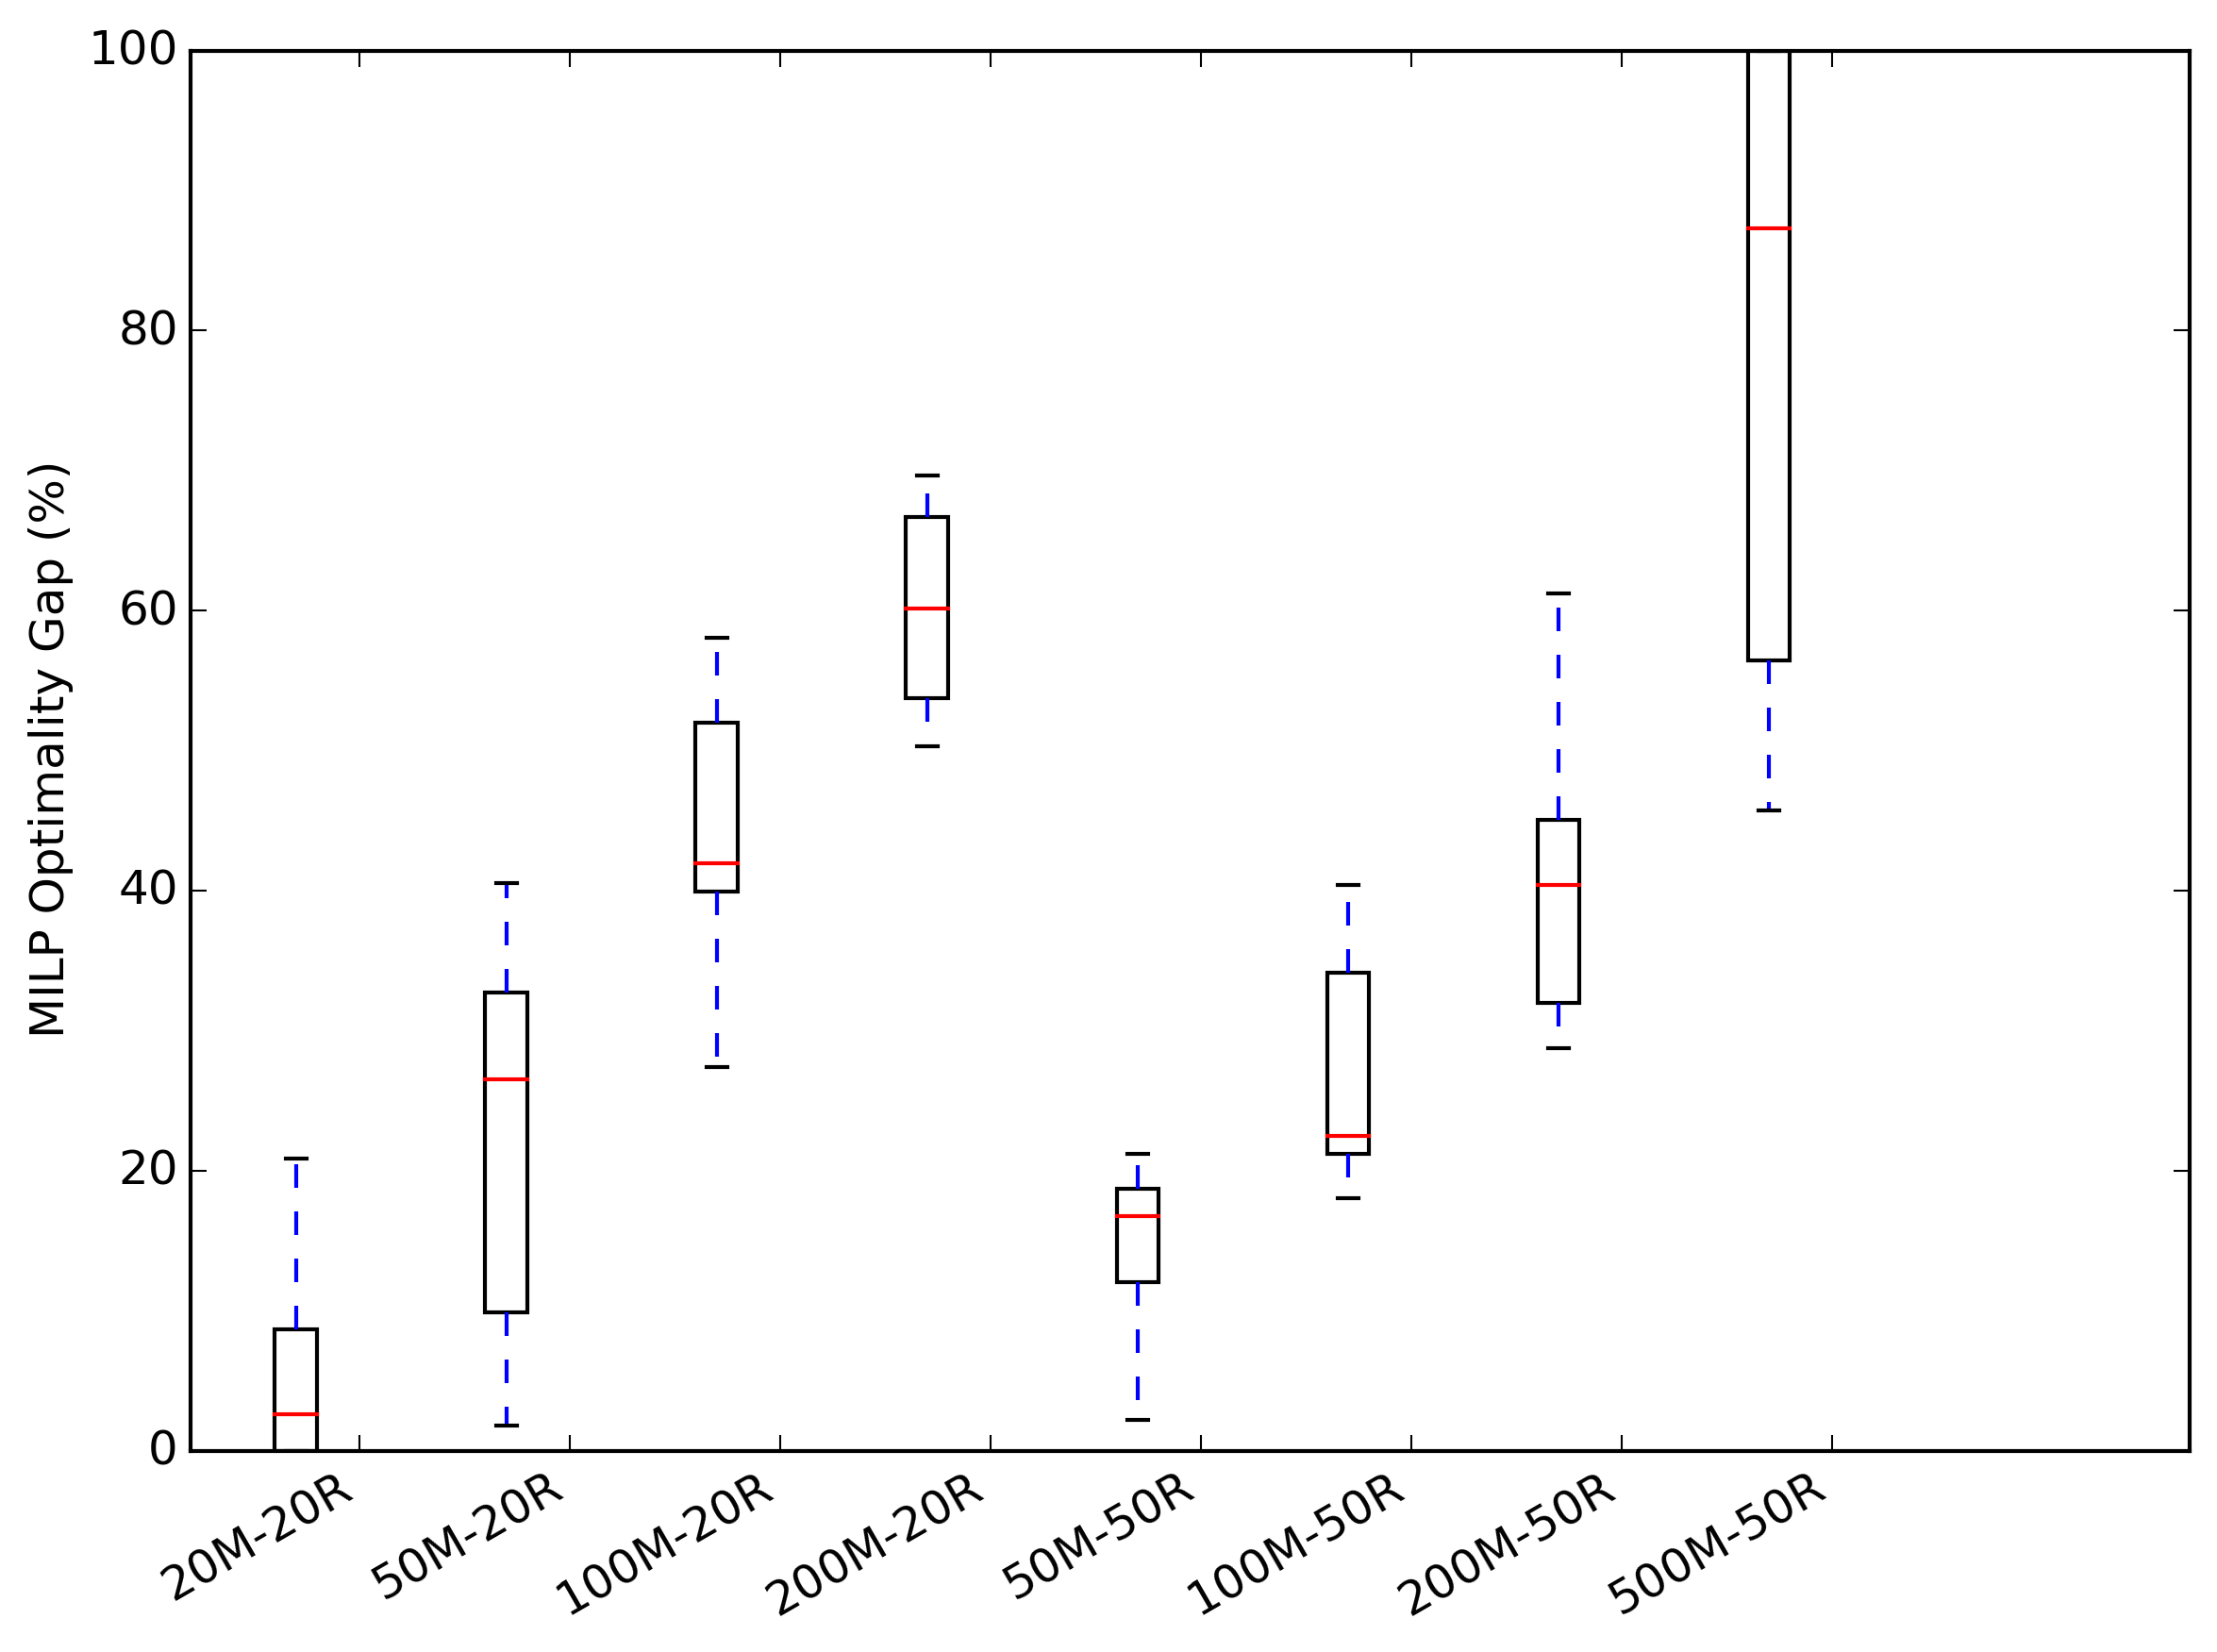
\includegraphics[width=0.9\linewidth]{figs/mip_optgap_maxdata500.png} \\
(a) MIP optimality gap \\[6pt]
		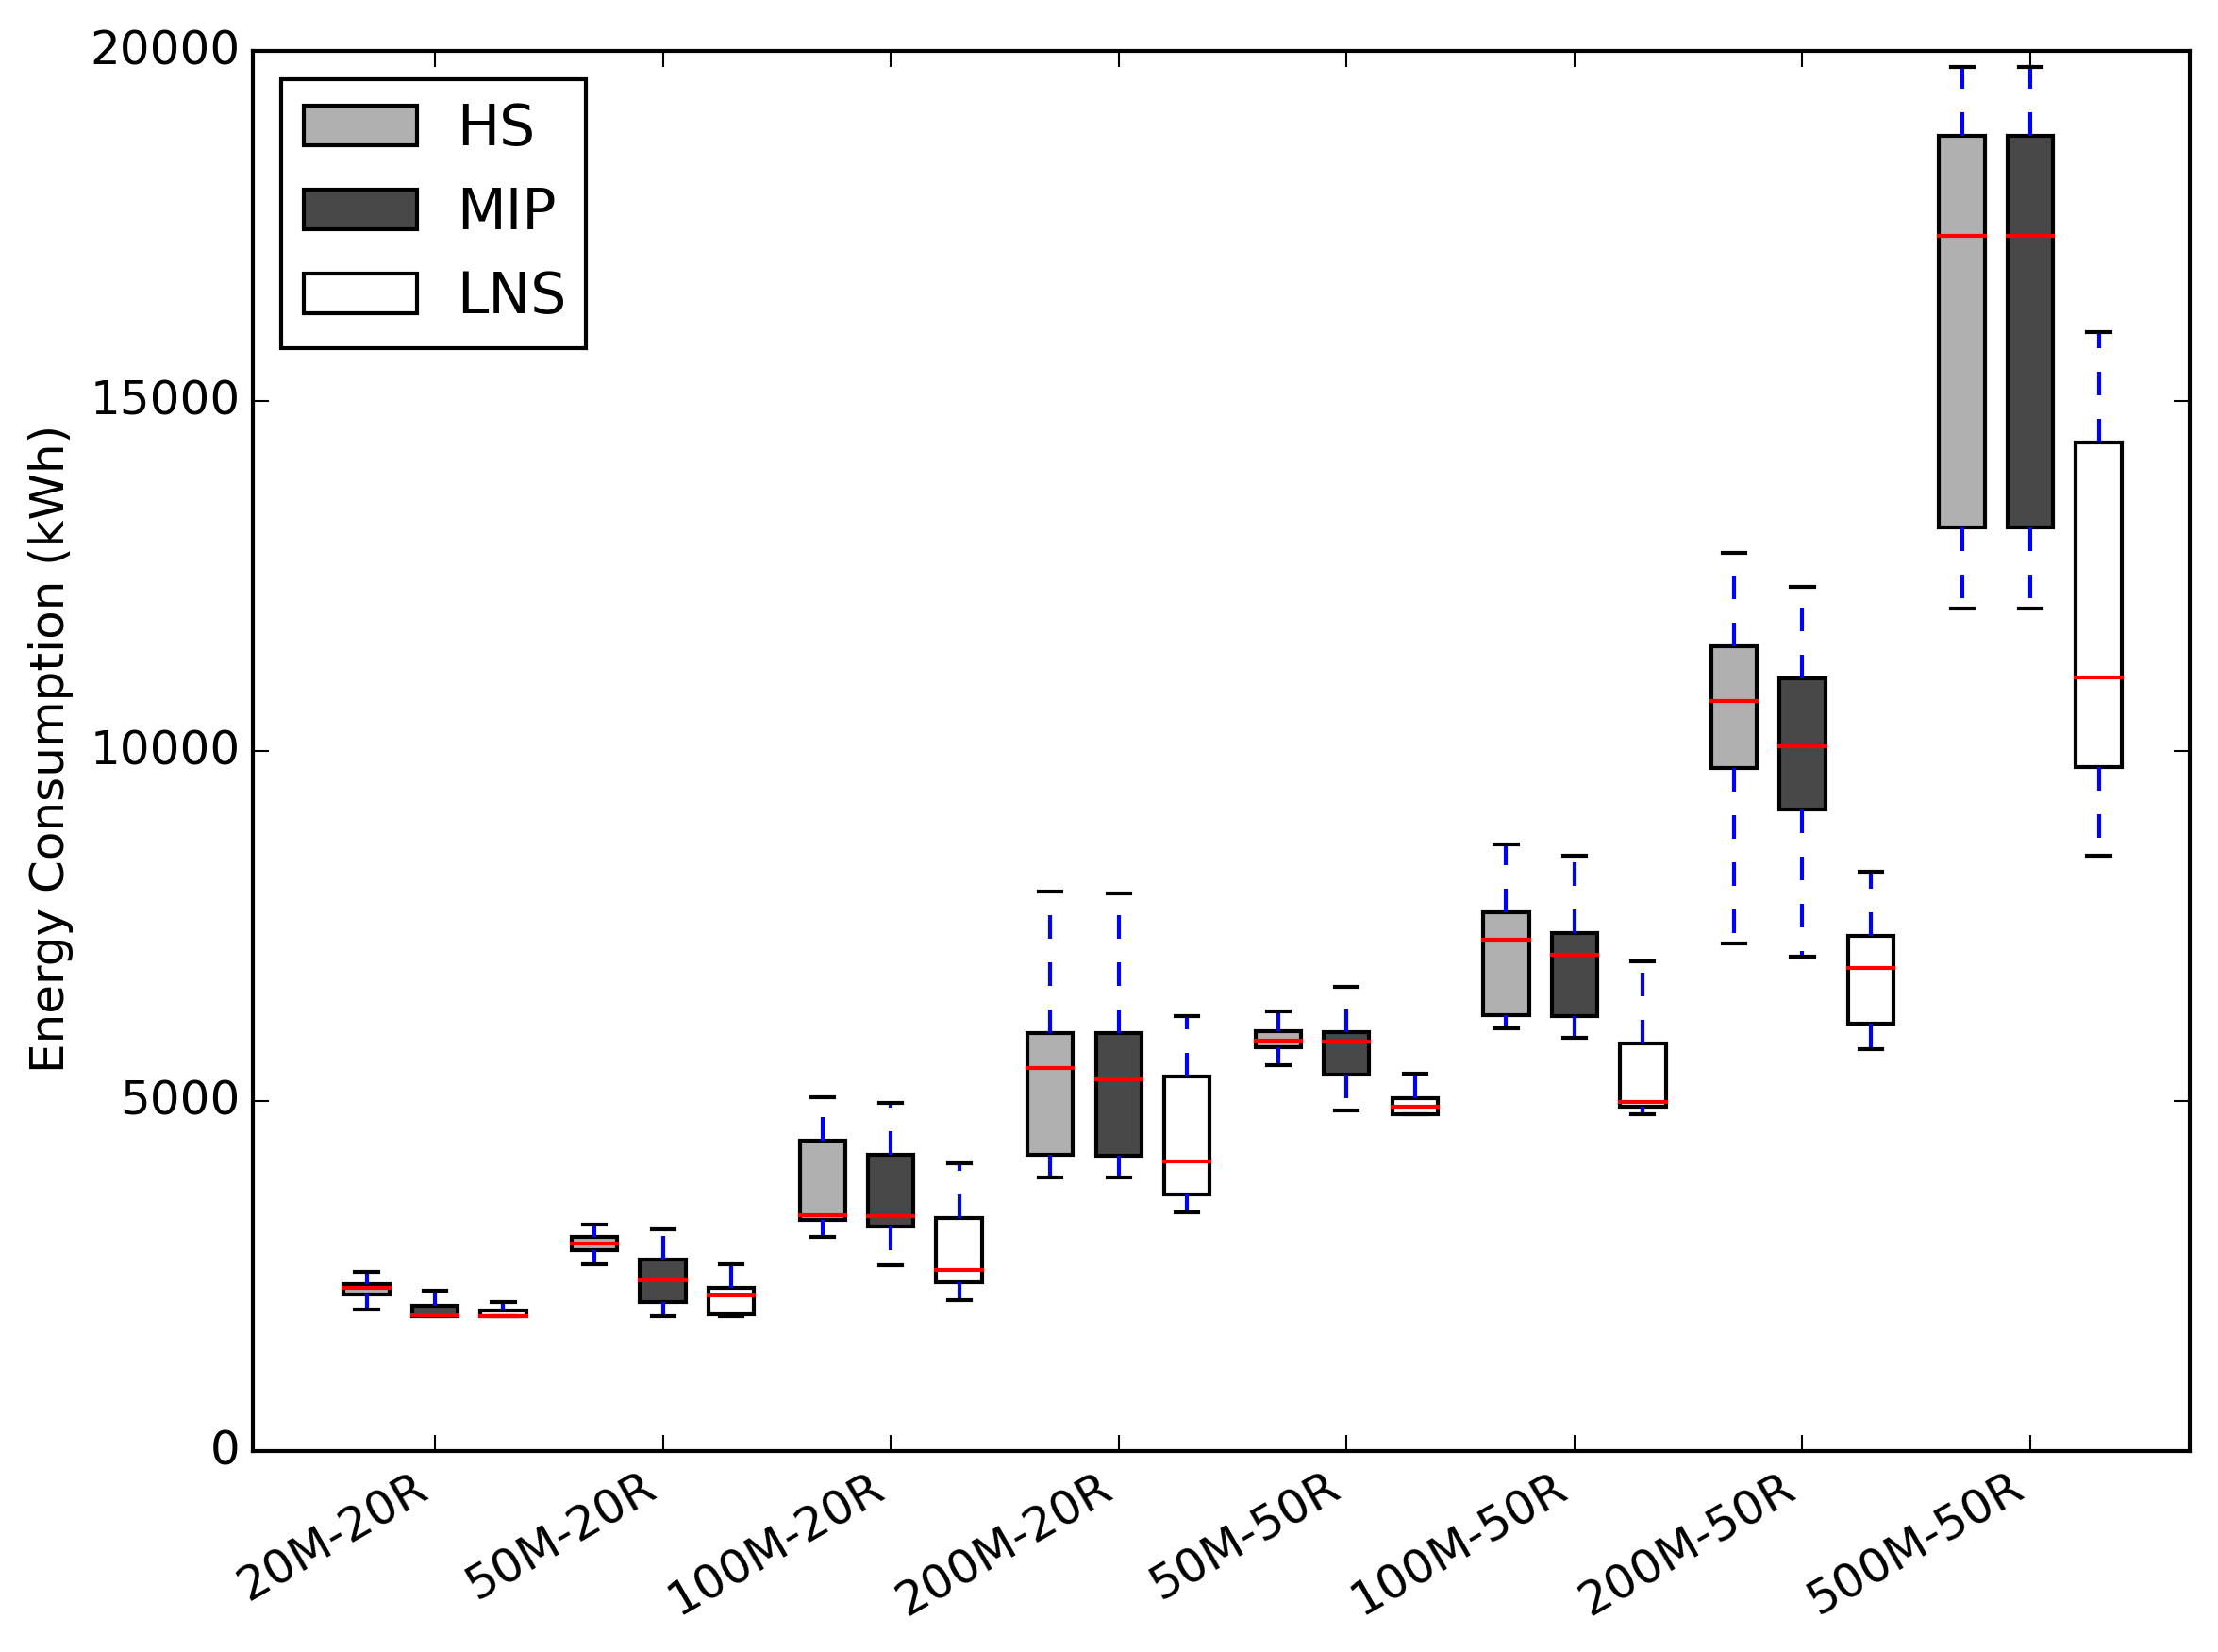
\includegraphics[width=0.9\linewidth]{figs/lnsmip_mspec_mspec900_shortHS_box_maxdata500.png}\\
(b) HS/LNS/MIP solution values \\[6pt]
	\caption{MIP optimality gap (top) and HS/LNS/MIP solution values (botton)}
	\label{fig:optgap}
\end{figure}

Figure \ref{fig:mspec_mspec_900} shows the performance improvement of MIP and LNS compared to the initial feasible solution, which is referred to as the heuristic solution (HS), over 500 runs. For each run, both the MIP and LNS approach were seeded with HS as an initial solution. Both MIP and LNS were given the same runtime limit of 15 minutes and HS was given 60 seconds. LNS was executed using the parameter configurations that were determined to be the best for each problem set. The results show that LNS significantly improves over MIP when given limited runtime. Overall, the improvement of LNS over MIP is between 14\% and 36\%. Note that in the largest problem instances, those in 500M-50R, MIP often fails to find even a slight improvement over the given initial solution HS in 15 minutes.

We reran all problem instances in Figure \ref{fig:mspec_mspec_900} using the AllM-AllR parameter settings. In this case, the performance of LNS decreased by 1 to 2\% for each problem set. Hence, instance specific algorithm configuration did have some impact, but even without it LNS performed significantly better than MIP.

Figure \ref{fig:optgap} provides insight into the optimality gap of the MIP approach and in the variation in solution quality. The MIP optimality gap after 15 minutes runtime is shown Figure \ref{fig:optgap}(a). Each box shows the median and the upper and lower quantiles of the optimality gap. The endpoints indicate the maximum and minimum. As observed previously the MIP approach fails to converge on the larger problem instances. Moreover, as can be seen from the figure, MIP's performance substantially degrades as problems become more constrained and exhibit a higher number of meetings to number of rooms ratio.

The variation in solution quality is shown on Figure \ref{fig:optgap}(b). The median of LNS always falls below the lower quantile of MIP. We note, however, that for the smallest problem instances in 20M-20R, MIP and LNS have almost similar performance. For even smaller problem instances MIP tends to be very effective, which is exactly why we have combined the two. We believe that the combination of LNS and MIP is especially good when considering highly constrained problems. LNS is used to destroy and repair the solution space and MIP is used to find a good local solution, possibly a locally optimal solution, in a short amount of time.



%\begin{figure}[h]
%\centering
%\begin{tabular}{cc}
%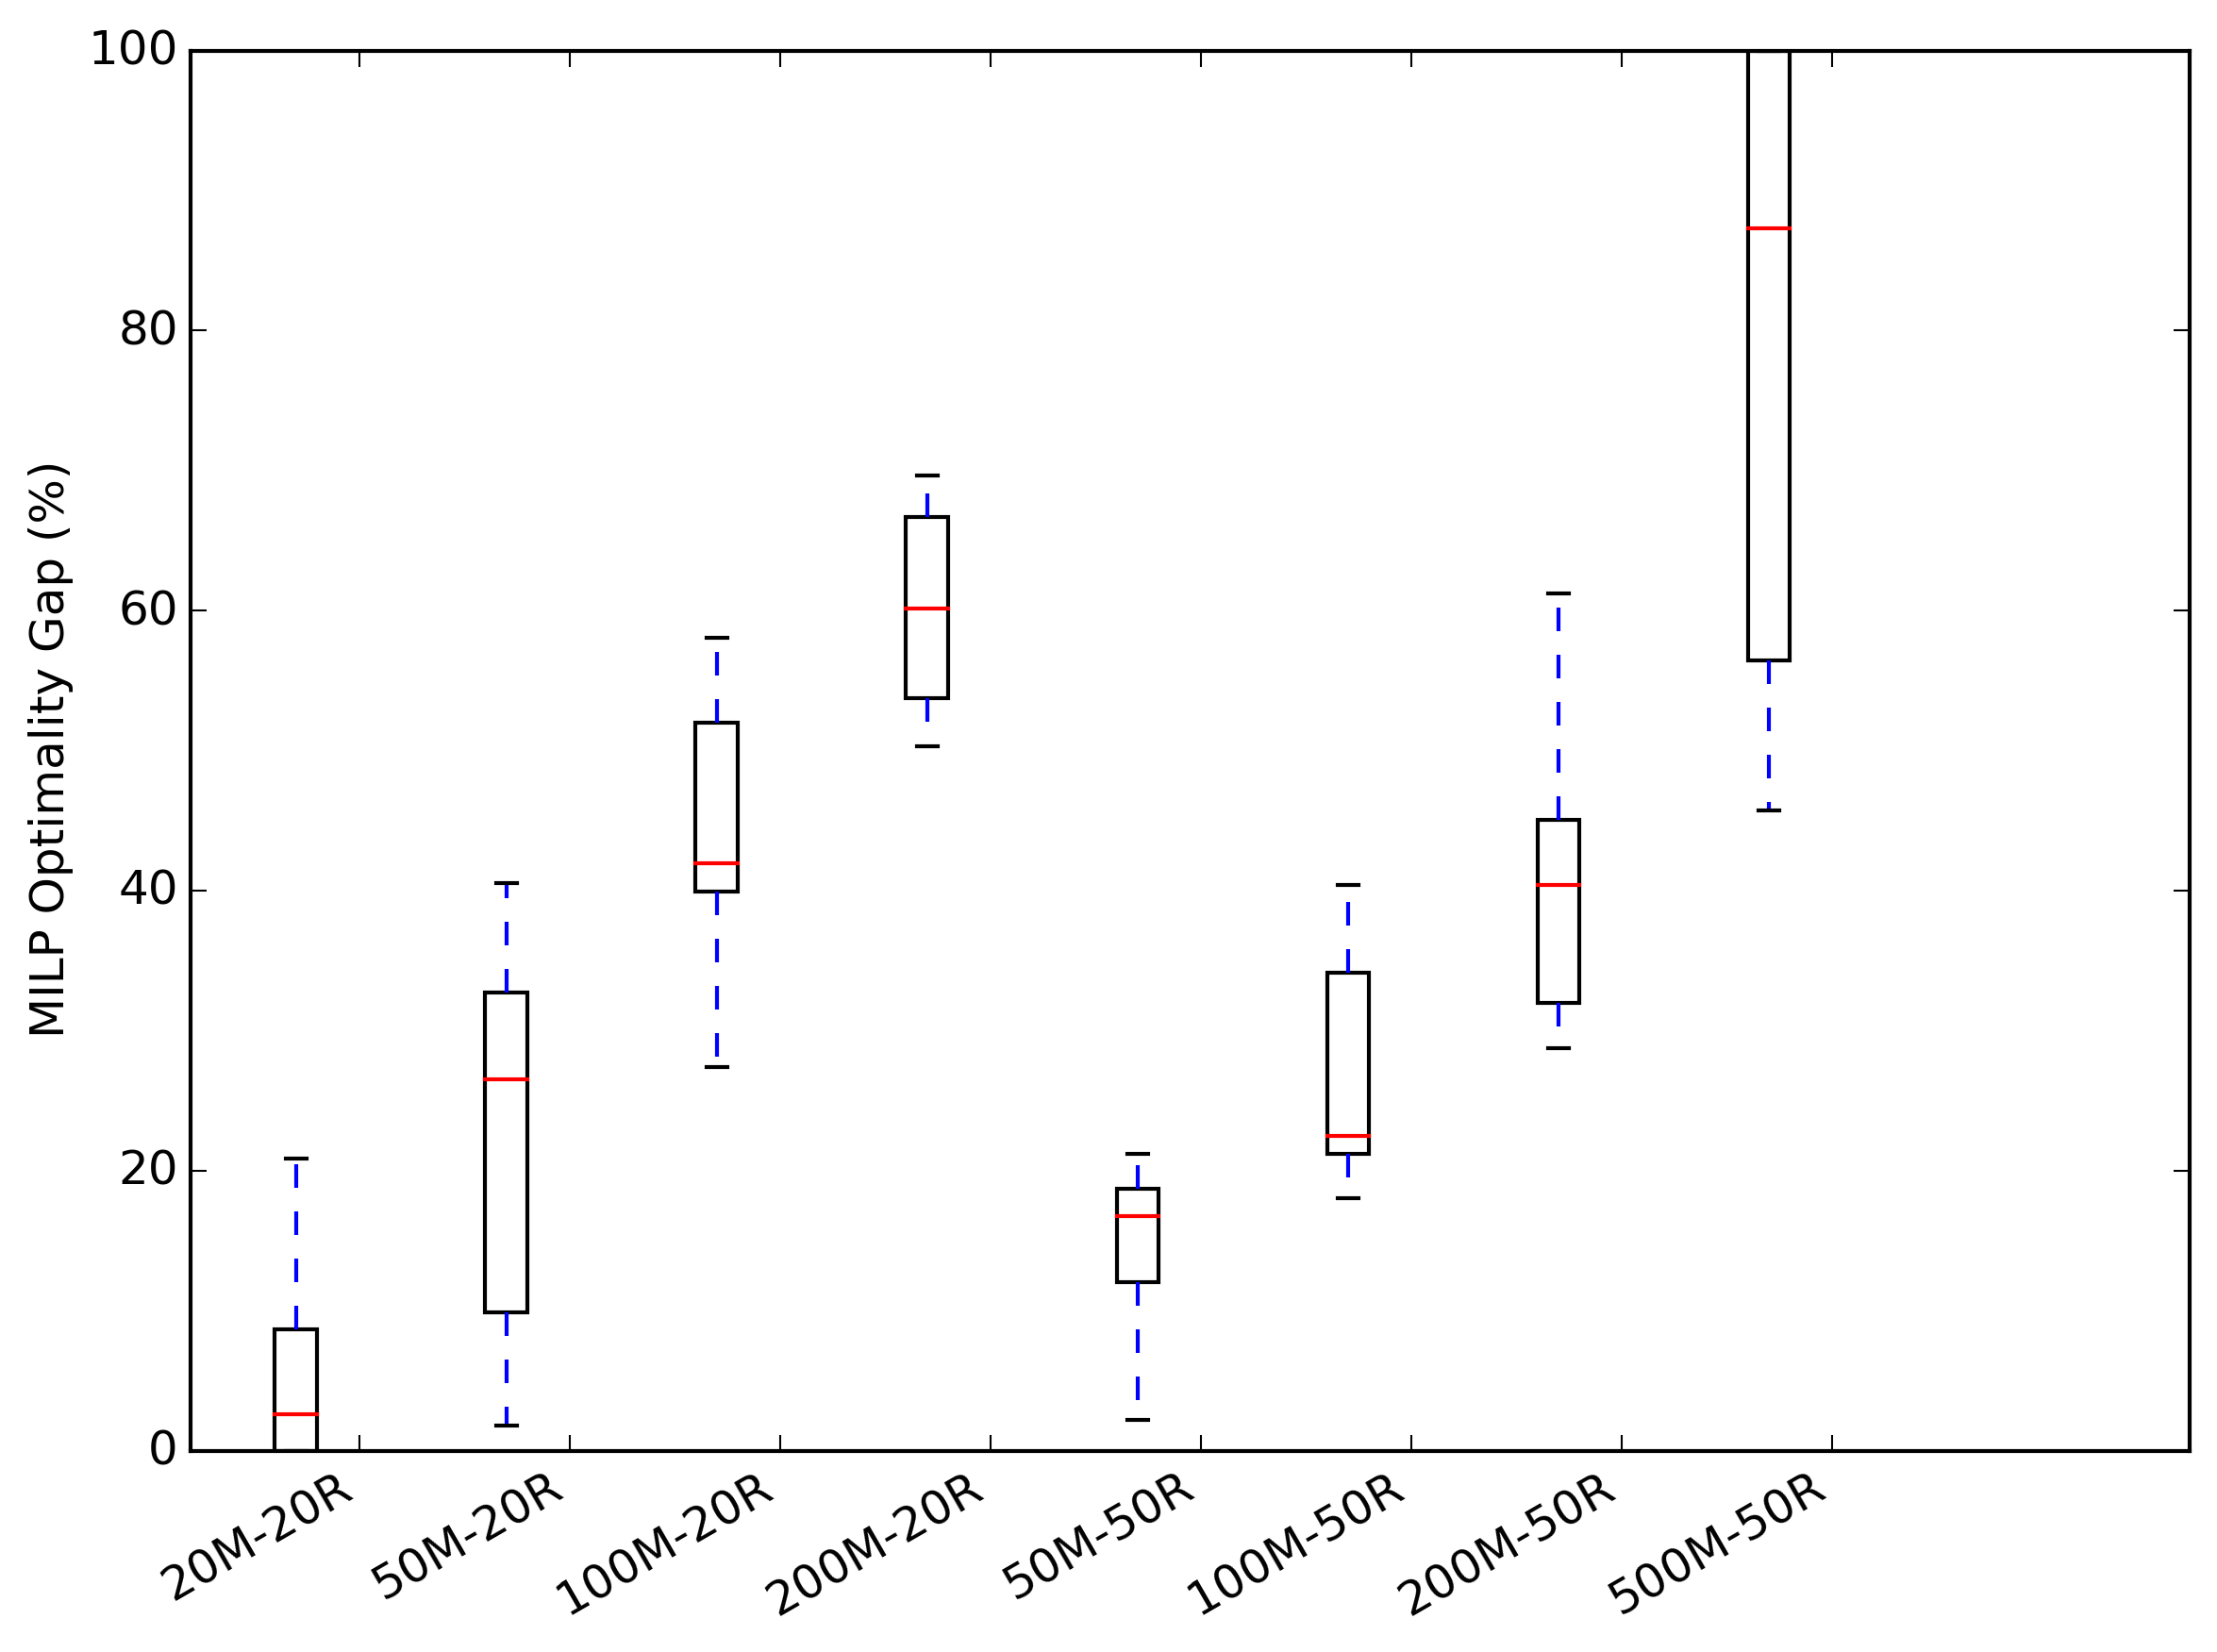
\includegraphics[width=2.3in,keepaspectratio]{figs/mip_optgap_maxdata500.png} &
%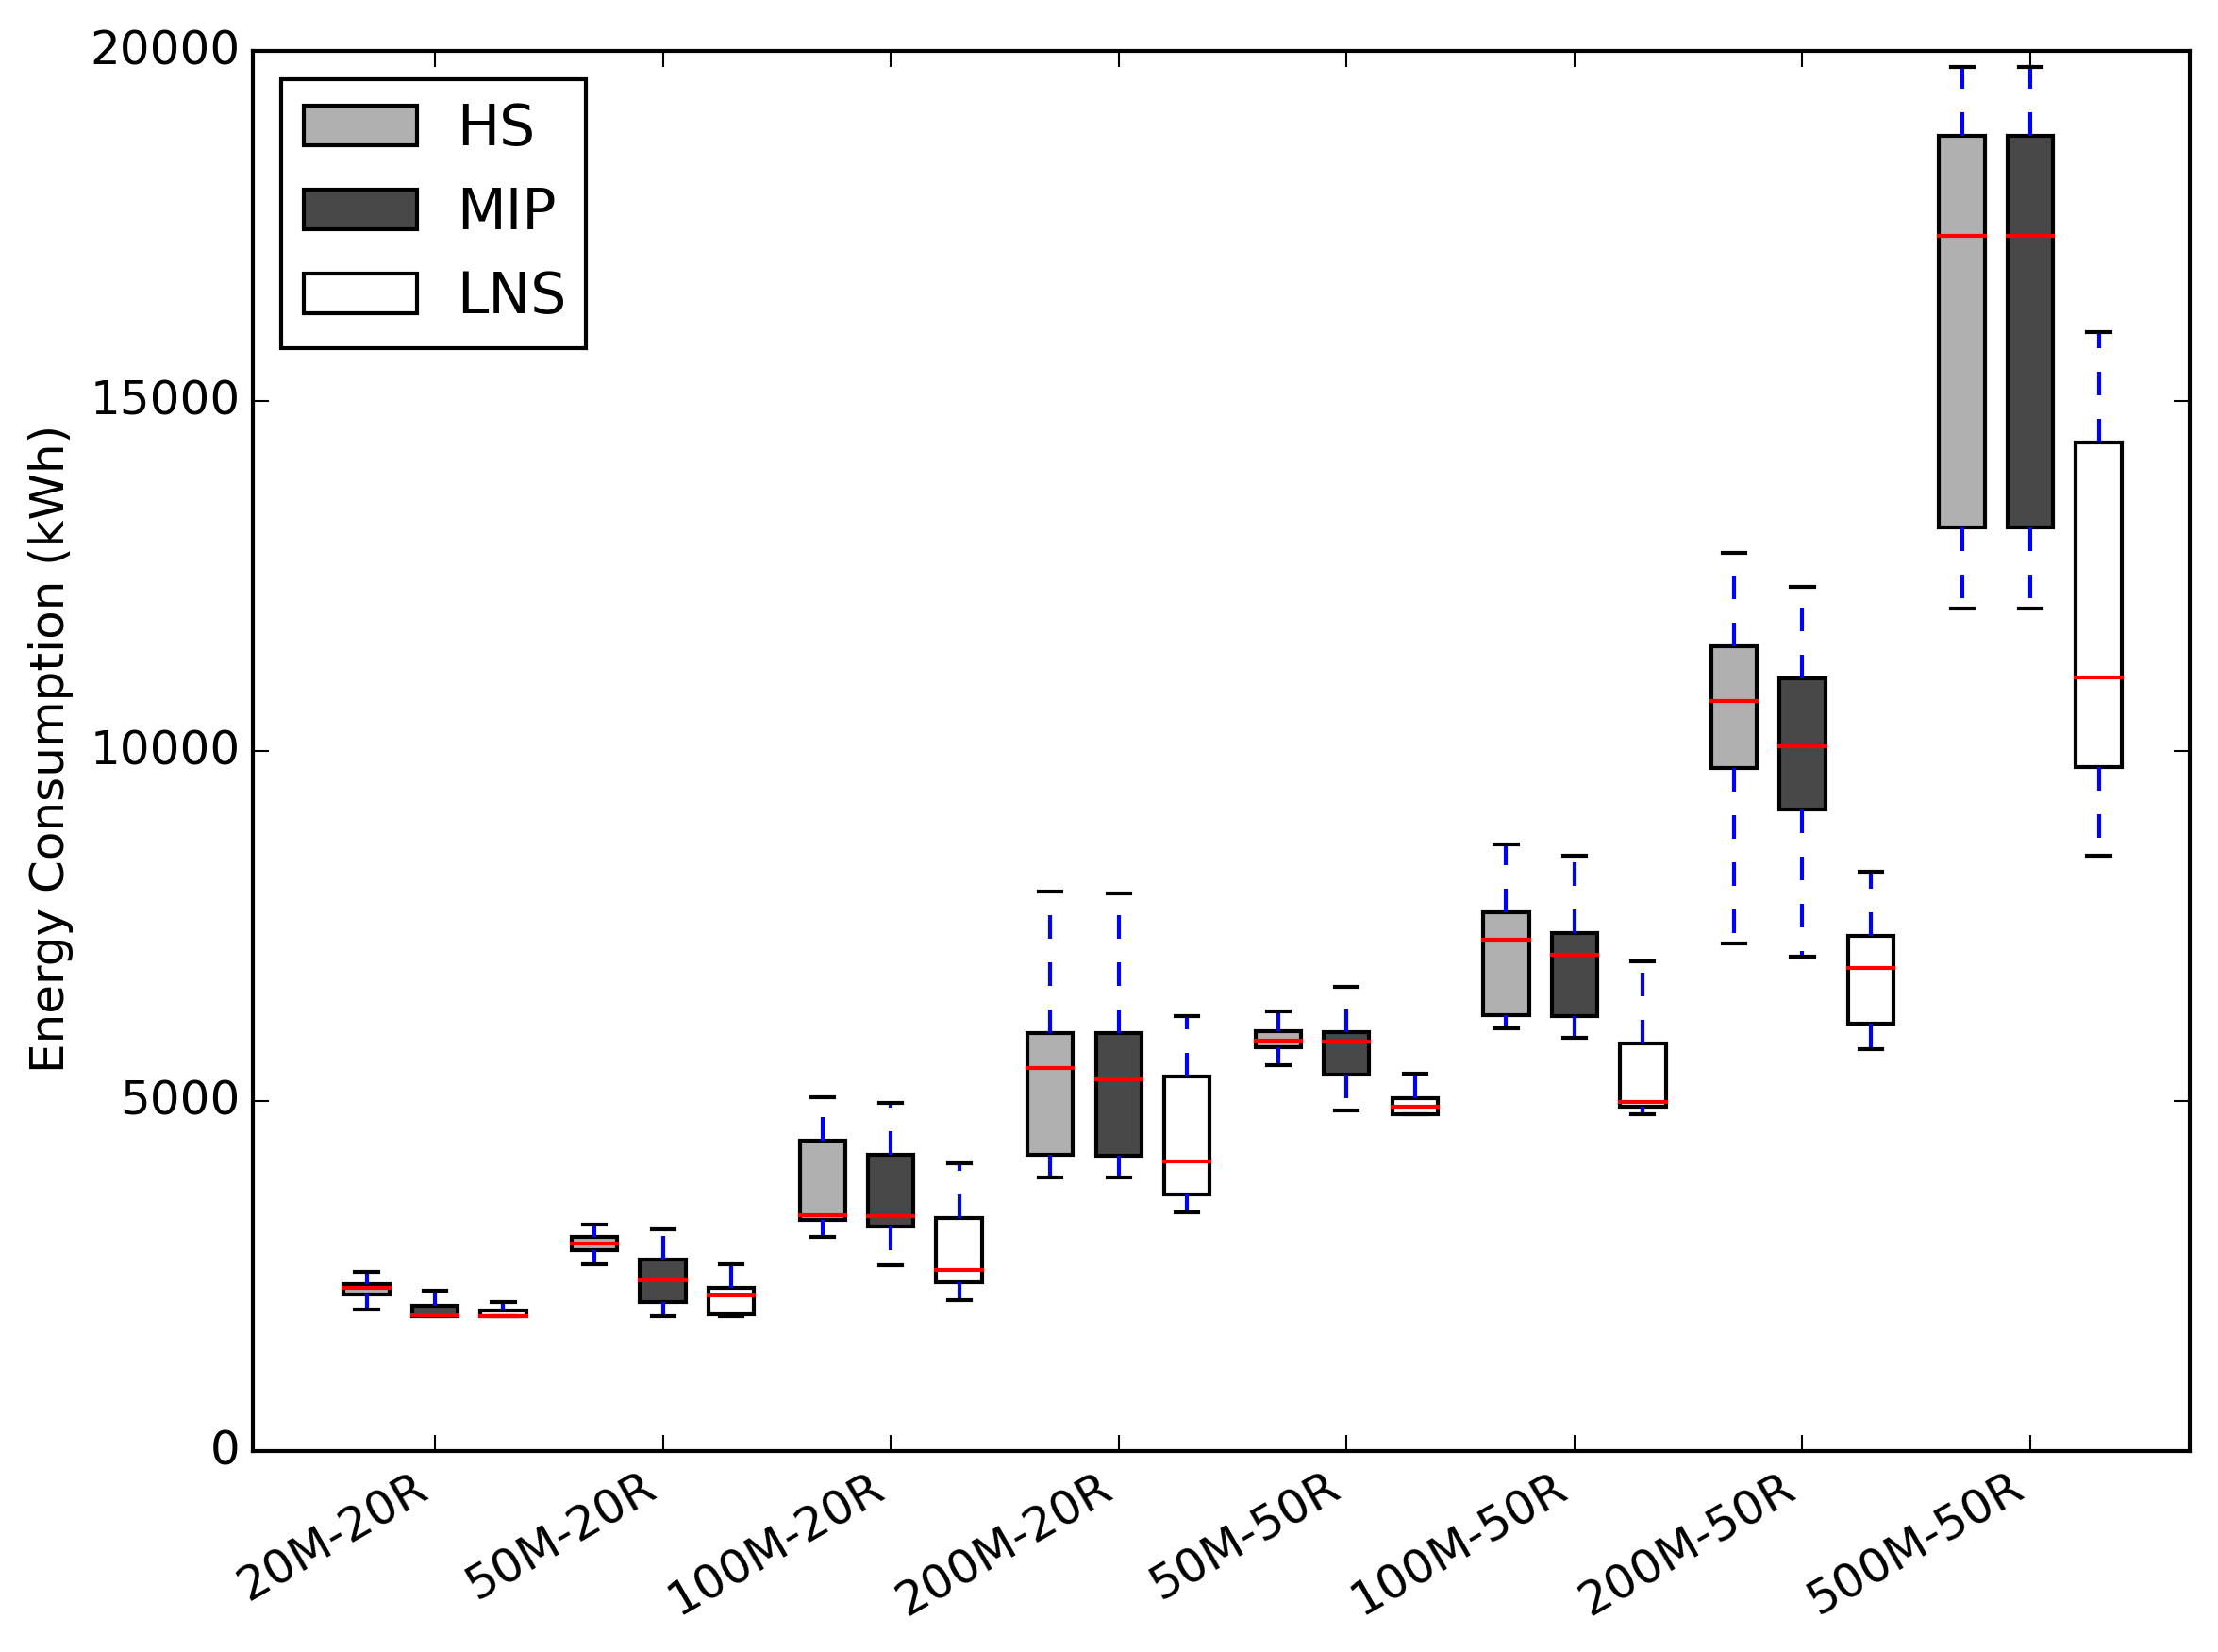
\includegraphics[width=2.3in,keepaspectratio]{figs/lnsmip_mspec_mspec900_shortHS_box_maxdata500.png} \\
%\end{tabular}
%\caption{MIP optimality gap (left) and HS/LNS/MIP solution values (right)}
%\label{fig:optgap}
%\end{figure}


\section{Related Work}\label{sec:related_work}

In Chapter \ref{cha:milp} we combine MPC with meeting scheduling and propose a MIP-based solution. This model achieves significant energy reduction when compared to approaches similar to those presented in \cite{goyal2013occupancy,kwak2013tesla,majumdar2012energy}. The drawback of this approach is that it does not scale well, which is why we developed a hybrid solution that combines MIP with LNS \citep{lim2015large}. %In \cite{lim15hvac}, we presented some of the initial results on applying LNS on this problem.  Here, we significantly expand on the details of the LNS algorithm, and present extensive results supporting the quality of the algorithm.

Also limited by the scalability of MIP, existing work on energy-aware scheduling only consider a small number of meetings or rooms. For example, \cite{chai2014minimizing} consider only 30 meetings in 9 rooms. \cite{kwak2013tesla} solves a total of 300 meetings per day in 35 rooms, but in an online manner where the MIP model needs to be solved at every session is relatively smaller. The other work resorts to heuristics-based approaches that generate a feasible solution in a reasonably short period of time but do not guarantee optimality. For instance, \cite{pan2013minimizing} examine up to 800 meetings in 150 rooms with their greedy scheduling algorithm. Likewise, \cite{majumdar2016characterising} only consider up to 12 meetings in 4 rooms due to the computational overhead incurred by feeding their schedules into building energy simulation software Energy+ \citep{crawley2000energyplus} for the calculation of HVAC consumption. Our work overcomes the limitations of these approaches by combining MIP with LNS, and by solving each sub-problem to optimality or near-optimality using a MIP-based integrated HVAC control and occupancy scheduling model. %scale well even for large instances.

There are techniques such as local branching or relaxation induced neigbourhood search (RINS) \citep{danna2005exploring,danna2003structured}, which apply local search to MIP. RINS forms a \textsl{domain-independent} neighbourhood in MIP. At every $n$th node of the MIP global branch-and-bound process, a MIP model is formed by fixing the value of the variables that have the same value in the current incumbent and the current continuous relaxation, and by solving on the remaining variables. The node limit $n$ is imposed to truncate the MIP optimisation when $n$ nodes have been explored in the search tree. 
% https://www.ibm.com/support/knowledgecenter/SS9UKU_12.5.0/com.ibm.cplex.zos.help/UsrMan/topics/discr_optim/mip/heuristics/45_rins.html
% Relaxation induced neighbourhood search (RINS) is a heuristic that explores a neighbourhood of the current incumbent solution to try to find a new, improved incumbent. It formulates the neighbourhood exploration as another MIP (known as the subMIP), and truncates the subMIP optimisation by limiting the number of nodes explored in the search tree.
In constrast, our model leverages a \textsl{domain-dependent} knowledge that forms a neighbourhood search strategy based on building zones and solves the joint HVAC control and occupancy scheduling sub-problem to optimality. The strength of our LNS model is that it allows a large neighbourhood to be explored using domain-dependent information whereas local branching or RINS explores a neighbourhood of the incumbent without using domain-dependent information. Moreover, RINS focuses on finding a good feasible solution instead of proving optimality. 
%   Note, we have not tried local branching on this problem, so this is something to test in future work.
% \cite{danna2003structured} --> In the literature, choosing related variables is most often achieved b taking advantage of the known high level structure of the specific problem at hand. Relaxation induced Neighborhood Search RINS) was introduced: it is a form of LNS that only relies on the continuous relaxation of the MIP model of the problem to define its neighbourhood. It can be used on any MIP model without any other input than the model itself. We want to investigate how a generic approach like RINS compares to a domain-dependent approach.
% combine structure and unstructured LNS (destroy room + RINS) - Use the LP relaxation to choose a neighbourhood Relaxation Induced Neighborhood Search (RINS) [Danna, Rothberg, Le Pape, 2003]

Parameter tuning is one important aspect of LNS. The values of the parameters of a LNS algorithm can impact the solution quality. These include the size of the neighbourhood, thresholds in terms of run time limit, node limit or solution limit etc. These parameters can be tuned based on knowledge of experts, or using an automated procedure. While we have only four configurable parameters in our LNS algorithm, it is impractical to examine all configurations. We resort to automated parameter tuning that adopt machine learning techniques.  Various parameter tuning software exist to automate the tuning process \citep{thornton2013auto,bergstra2012random, hutter2011sequential}. We use SMAC \citep{hutter2011sequential} to train our LNS parameters automatically and identify a global configuration that are optimum to tackle multiple instances of different features and properties. 
Note that SMAC has been used to train parameters in various applications such as kidney exchange matching \citep{dickerson2015futurematch}, medical imaging \citep{angermueller2016deep} and social network analysis \citep{vaswani2016adaptive} etc., but is first used here to train parameters in energy aware scheduling in smart buildings.

Combining constraint-based methods with neighbourhood search methods is not new. For example, \cite{lebras2013robust} use LNS with MIP in network design for a species conservation problem, \cite{gaspero2013constraint} use LNS with CP in balancing bike sharing systems, \cite{rendl2012hybrid} apply CP with variable neighbourhood search for home-care scheduling, \cite{mehta2012comparing} use both MIP and CP-based LNS approach for machine reassignment problem, \cite{bent2004two}, \cite{kilby2011flexible} use LNS with CP to solve vehicle routing problem, \cite{mitrovicminic09local} apply variable neighborhood search to the multi-resource generalized assignment problem. LNS is also widely used as a technique to solve complex timetabling problems \citep{meyers2006very,abdullah2007investigating,burke2010hybrid}, nurse rostering problems \citep{bilgin2012local} and shift-scheduling problems \citep{quimper2010large}. We are, however, unaware of its application in the space of energy aware scheduling in smart buildings.



\section{Conclusion and Future Work}\label{sec:lns:conclusion}

In this chapter we extend our work in Chapter \ref{cha:milp} which introduced a MIP model for energy aware meeting scheduling. The MIP model that is described previously only solves problem instances that involve a small number of meetings and rooms. We combine MIP with LNS % in order to scale to larger problems. 
and show that by embedding MIP model into a large neighbourhood search, we can scale to timetabling problems of practical relevance.

We developed a heuristic to generate an initial feasible solution quickly, which we use to warm start both the MIP and LNS approach. In our experiments, the most effective neighbourhood was one that destroys and repairs all meetings scheduled in 2 to 4 rooms. The resulting subproblem was small enough for MIP to solve to (near) optimality and, at the same time, large enough to explore alternate solutions. We studied the performance of MIP and LNS and demonstrated the potential of our LNS approach for effectively tackling large-scale HVAC control and meeting scheduling problems. The LNS achieves 14 to 36\% better energy savings than the MIP approach when both given a runtime of 15 minutes. 
%In order to provide an absolute sense of the solution quality, we plan to evaluate our schedules with the EnergyPlus simulator.

In future, we are interested in exploring new algorithmic approaches that allows us to scale even further. We are particularly interested in investigating symmetry breaking in MIP \citep{ostrowski2015modified}. Symmetries lead to a large number of equivalent solutions, which causes branch-and-bound to be ineffective. While we dealt with symmetries due to meetings with similar characteristics by introducing meeting types, symmetries still exists in our MIP formulation due to rooms with similar characteristics. Introducing room types, however, may not be possible because room temperature at time step $t$ is dependent on time step $t-1$. In future work, we aim to identify branching strategies that can better deal with symmetries in our MIP formulation, for example, by assigning different branching priority to variables $x_{m,l,k}$ such that rooms with different energy consumption are explored first. %On top of that, most of the existing optimisation solvers \citep{gurobi, cplex2009v12} provide a configurable symmetry breaking parameter that, once activated, automatically detect and remove symmetries. It might be interesting to activate this parameter while running the repair step.

We will also further investigate incorporating RINS-based local branching to our LNS model. This can be achieved by activating RINS  heuristics in MIP solvers such as \cite{gurobi}. It will be interesting to compare the solution quality of these approaches.
For the initialization stage of LNS, it might also be possible to formulate the initial schedule using different heuristics, modeling and solving technique such as CP. 



%Moreover, we are also interested in investigating an online stochastic approach to our HVAC control and meeting scheduling problem. Such an approach can deal with current requests, future requests, changes and cancelation of requests, but also with the uncertainty around outdoor air temperature and weather conditions.

%This approach may also be further enhanced to incorporate dynamic temperature bounds to adjust thermal comfort based on outdoor temperature. %It is expected to greatly reduce the energy consumption while improving the solution feasibility.


%TODO:
%   Experiments - Feas % x tf x cvs 
%		Add figure to illustrate online schedule with auto update HVAC
%		Add more experiments of online?  ---- impact of cvs and tf in online scenario 
%		Add online scheduling literature
%		Add stochastics as future or ??

%   The model should be able to handle impromptu scheduling request and response in time in an \emph{online} manner.

\chapter{Handling Online Requests}
\label{cha:online}

\section{Introduction}

In Chapter \ref{cha:lns}, we presented a scalable joint HVAC control and occupancy scheduling model by combining MIP and LNS. Within a short computational time, this model is capable of minimising HVAC utilisation by scheduling an extensive number of group activities to take place at a large number of building zones and time slots.
However, this approach was offline and assumes all activities to schedule and other parameters such as the weather forecast and solar gains are known in advance. Although the model generates energy-efficient schedules, its practicability is nevertheless limited in the real-world. In reality, scheduling requests can arrive at any time of the day using existing room booking systems. 
In a recent survey, \cite{kwak2013tesla} shows that 56\% of meeting requests were made within one day before the actual meeting day. Thus, the ability to handle dynamically arriving requests is crucial. Moreover, the ability to update HVAC control following a change in weather forecast is also important. 

In this chapter, we extend the HVAC-aware occupancy scheduling approach to process activity requests in an \textsl{online} manner. In more detail, we present an online approach that models and solves the joint HVAC control and occupancy scheduling problem. The model needs to be responsive to dynamic information such as new activity requests and weather updates. Our online algorithm greedily commits to the best schedule for the latest activity requests and notifies the occupants immediately, but revises the entire future HVAC control strategy each time it considers new requests and weather updates. This allows the integrated model to handle incoming requests in a prompt manner whilst continuously optimising the HVAC control reflecting updated weather forecast and activity schedules. In our experiments, the quality of the solution obtained by this approach is within 1\% of that of the clairvoyant solution. 

In the next section, we show how our integrated model is being transformed into an online model. We further elaborate on how the online model is scaled with the LNS method. In Section \ref{sec:online:experiments} we compare our model with the clairvoyant solution, showing the efficacy of this simple and effective online algorithm. We discuss about related work in Section \ref{sec:online:related_work}. We then conclude the chapter %and discuss potential future works 
in Section \ref{sec:online:conclusion}.


\section{Online HVAC-Aware Occupancy Scheduling} \label{sec:online:sche_model}

This section presents our online occupancy scheduling and HVAC control problem. We start by describing the online setting and our notations. We then cover the scheduling constraints and variables which, later on, will interact with the HVAC control model to form the complex joint scheduling and control model. Following our work from the previous chapters, we formulate our model as a MIP. It can be solved using a MIP solver, or when scaling up to problems of practical size, by combining MIP with LNS.

In our online setting, the scheduler runs recurrently and each run is called an \emph{online session}. Each online session $i\in I$ starts at time $\tau_i$ and ends before the next session starts at time $\tau_{i+1}$. The scheduling and control model discretizes time into a set $K$ of {\em time steps}. Each time step $k\in K$ starts at time $t_{k}$. Two consecutive time steps $k$ and $k+1$ are separated by a fixed duration $t_{k+1}-t_{k} = \bm{\Delta_t} \in \mathbb{R}^+$. Each online session $i$ considers a horizon of $\bm{n}$ time steps $K(i) = \{k(i), \ldots, k(i)+\bm{n}-1\}$ where $k(i)$, the first time step in that horizon, is the least time step in $K$ such that $t_{k(i)} \geq \tau_i$. 

\subsection{Scheduling Model}
Let $L$ be the set of locations (or, interchangeably, zones) in the building, and $P$ be a set of participants. An activity request $m$ is a tuple $\langle \bm{a}_m, K_m, L_m, P_m, \bm{d}_m \rangle$ where $\bm{a}_m \in \mathbb{R}^{+}$ is the request arrival time, $K_m\subseteq K$ is the set of time steps at which the activity is permitted to \underline{start} in the future (for each $k\in K_m, \bm{a}_m < t_k$), $L_m\subseteq L$ is the set of locations at which the activity is permitted to take place, $P_m\subseteq P$ is the set of attendees for the activity and $\bm{d}_m \in \mathbb{N}$ is the activity duration (number of time steps). As in the previous chapter, note that the sets $K_m$ and $L_m$ can be used to encode a variety of situations, such as room capacity requirements, availability of special equipment such as video conferencing, time deadlines for the activity, and attendee availability constraints. We write ${\cal C}(M)$ for the set of attendee conflicts w.r.t. a set of requests $M$; each conflict $C$ is a subset of requests, each pair of which has at least one attendee in common: ${\cal C}(M)=\{C\subseteq M \mid \forall m,m'\in C, P_m\cap P_{m'} \neq \emptyset \}$.

To account for all activities that have been scheduled so far, we maintain a master schedule $S$ as a set of triples $\langle m, l,k \rangle$ storing the activity request id $m$, the assigned location $l$, and the time step $k$ at which $m$ is scheduled to start. 
At each online session $i$, the scheduler schedules the new activity requests $N(i)$ which have been received since the start of session $i-1$, i.e, each $m\in N(i)$ satisfies $\tau_{i-1} < \bm{a}_m \leq \tau_{i}$. It also needs to consider, without modifying them, the set $Q(i)$ of ongoing activities and future activities that were scheduled during previous sessions: $Q(i) =\{m \mid \exists \langle m,l,k \rangle \in S\mbox{~such that~} k +\bm{d}_m -1 \geq k(i)\}$.
So overall, the set of activities to consider at session $i$ is $M(i) = N(i) \cup Q(i)$. To simplify the scheduling model below, we assume that for each pre-scheduled request $m \in Q(i)$ such that $\langle m,l,k \rangle \in S$, the set of permissible locations is reduced to $L_m =\{l\}$, and the set of permissible start time steps is reduced to the scheduled start time $k$ or the first time step $k(i)$ of the session, which ever occurs last, i.e. $K_m = \{\max(k,k(i))\}$. For consistency, the meeting duration $\bm{d}_m$ is decremented by $k(i)-k$.

\begin{figure}[t]
\centering
\includegraphics[width=5in,keepaspectratio]{figs/timeline.jpg}	
\caption{Online scenario}
\label{fig:timeline}
\end{figure}

Fig.~\ref{fig:timeline} shows a scenario example featuring three requests $m_1, m_2$ and $m_3$ with arrival times $\bm{a}_1$, $\bm{a}_2$ and $\bm{a}_3$, respectively. The set of locations is $L=\{{\bm l}_1,{\bm l}_2\}$. The dash vertical lines show the start of the sessions, and the dotted vertical lines delimit the time steps. In this instance, the scheduler runs every 10 minutes and the time steps are 30 minutes long. At the start of session $i=302$, requests $m_1$ and $m_2$ have already been scheduled and $m_3$ is a new request,
hence $N(302) = \{m_3\}$, $Q(302) = \{m_1,m_2\}$. The master schedule is $S=\{\langle m_1, {\bm l}_1, 102\rangle, \langle m_2, {\bm l}_1, 100\rangle\}$, and the first time step of the new session is $k(302) = 101$. The set of permissible locations and start time steps for the new request are $K_3=\{101,102\}$ and $L_3=\{{\bm l}_1,{\bm l}_2\}$ (${\bm l}_1$ will be ruled out by the scheduler).
Those of the pre-existing requests are reduced as follows: $L_1 =\{{\bm l}_1\}, K_1=\{102\}, L_2 = \{{\bm l}_1\}$ and $K_2 =\{101\}$. 

We are now ready to describe our scheduling constraints and variables for online session $i$. Similarly, as defined in the previous chapter, the main scheduling variable is the boolean decision variable $x_{m,l,k}$ which is true iff request $m\in M(i)$ is scheduled to take place at zone $l\in L_m$ starting at time slot $k\in K_m$. We also introduce the variables $y_{m,l,k}$ which is true iff activity $m$ is scheduled to occupy location $l$ at time step $k$, $z_{l,k}$ which is true iff zone $l$ is occupied at time step $k$, and $pp_{l,k}$ which indicates the number of people in zone $l$ at time step $k$. These variables will be used by the HVAC control part of the model in Section \ref{sec:online_hvac_model}.

%The scheduling constraints are similar to the model presented in chapter \ref{cha:milp}, with an exception that the scheduling horizon $k$ changes for each online session $i$. 
Constraints \eqref{eq:online_ms_everytype} ensure that all requests are scheduled exactly once within the allowable start times and locations. $\psi_m$ represents the number of meetings of type $m$ with similar time windows, the same number of attendees, and the same attendee conflicts.
Constraints \eqref{eq:online_ms_y} define the $y_{m,l,k}$ variables. Constraints \eqref{eq:online_ms_totalalloc} state that no more than one activity can occupy a location at any time and define the $z_{l,k}$ variables. 
Constraints \eqref{eq:online_ms_totalnum} determine the number ${pp}_{l,k}$ of occupants at each location and time step, and finally constraints \eqref{eq:online_ms_meeting} ensure that activities with at least one attendee in common cannot be scheduled in parallel. 
Once a new request $m\in N(i)$ has been scheduled, the master schedule $S$ is updated by adding the 3-tuple $\langle m,l,k\rangle$ for which $x_{m,l,k} =1$.

\begin{align}
\mathop{\sum \limits_{l\in L_m, k \in K_m}} \hspace{-12pt} x_{m,l,k} &= \psi_m \hspace{10pt} \forall m \in M(i)  \label{eq:online_ms_everytype}  \\
%\mathop{\sum \limits_{l\in L_m, k \in K_m}} \hspace{-12pt} x_{m,l,k} &= 1 \hspace{10pt} \forall m \in M(i) \label{eq:online_ms_every} \\
\mathop{\sum \limits_{\substack{k' \in K_m: \\
l\in L_m, \hspace{5pt} k-\bm{d}_m+1 \leq k' \leq k}}} \hspace{-12pt} x_{m,l,k'} & = y_{m,l,k} \hspace{10pt} \forall m \in M(i), l \in L, k \in K(i) \label{eq:online_ms_y} \\
\mathop{\sum \limits_{m \in M(i)}} \hspace{5pt} y_{m,l,k} &\leq z_{l,k} \hspace{10pt} \forall l \in L, k \in K(i) \label{eq:online_ms_totalalloc} \\
\mathop{\sum \limits_{m \in M(i)}} y_{m,l,k}\times \left| P_m\right| &= {pp}_{l,k} \hspace{10pt} \forall l \in L, k \in K(i) \label{eq:online_ms_totalnum} \\
\mathop{\sum \limits_{m \in \nu,l \in L_m}} y_{m,l,k} &\leq 1 \hspace{10pt} \forall k \in K(i), \nu \in {\cal C}(M(i)) \label{eq:online_ms_meeting}
\end{align}

%Note that to simplify the model, the scheduling constraints for all ongoing activities and future activities $m \in Q(i)$ that were scheduled during previous sessions can be omitted. We may remove constraints \eqref{eq:online_ms_everytype}-\eqref{eq:online_ms_y} for these meetings and set \eqref{eq:online_ms_totalalloc} and \eqref{eq:online_ms_totalnum} to
%\begin{align}
%z_{l,k} &= 1 \hspace{10pt} \forall m \in Q(i), l \in L_m, k \in K^o_m \label{eq:ms_totalalloc_occ} \\
%\left| P_m\right| &= {pp}_{l,k} \hspace{10pt} \forall m \in Q(i), l \in L_m, k \in K^o_m  \label{eq:ms_totalnum_occ}.
%\end{align}
%\noindent where $K^o_m = \left\{K^o_m \subseteq K | \forall k \in K^o_m, m \in Q(i), l \in L_m, x_{m,l,k'} = 1, k = \left\{k'\!,\!k'+1\!,\! \ldots\!,k'\!+\!d_m\!-\!1\right\} \right\}$. Note that Constraints \eqref{eq:online_ms_meeting} can also be omitted for pre-scheduled meetings. This is achieved by removing all slots that are pre-occupied by the conflicting attendees. %while generating $\nu \in {\cal C}(M(i))$ for new meetings. 
%These steps greatly reduced the number of variables and constraints, avoiding unnecessary search in MIP.
  
\subsection{HVAC Control Model} \label{sec:online_hvac_model}

The HVAC control model is similar to the model presented in Chapter \ref{cha:milp}, with an exception that the scheduling horizon $k$ changes for each online session $i$. We use the reduced model which considers only external walls in Equation \eqref{eq:roomtemperature_lns}. Our goal is to generate energy-efficient schedules that minimise the energy use of air-conditioning, re-heating and fan operations of the HVAC, considering all on-going, future and new meetings known upon the online session $i$ starts. Thus, similar to before, the objective function for each session $i$ is the following.

\begin{equation} 
\mbox{minimise} \sum_{k\in K(i)}  \left( p_{k}^{cond} + p_{k}^{fan} + \sum_{l \in L} p_{l,k}^{heat}\right) \times \bm{\Delta_t}
\end{equation}
where
\begin{align}
p_{k}^{fan} &= \bm{\beta} \sum_{l \in L} a_{l,k}^{SA} \quad  \forall k \in K(i) \label{eq:online:p_fan} \\
p_{k}^{cond} &= \bm{C^{pa}}\left(\bm{T_{k}^{OA}}(i) - \bm{T^{CA}}\right) \sum_{l \in L}  a_{l,k}^{SA} \quad \forall k \in K(i) \label{eq:online:p_cond} \\
p_{l,k}^{heat} &= \bm{C^{pa}} (T_{l,k}^{SA}- \bm{T^{CA}}) a_{l,k}^{SA} \quad \forall l \in L,k \in K(i) \label{eq:online:p_heat}
\end{align}

In Constraints~(\ref{eq:online:p_cond}), we assume that online session $i$ uses the latest update $T_{k}^{OA}(i)$ available for the outdoor temperature forecast at each time step $k$. 
The temperature at each zone and time step, and the effects of the HVAC control on this zone temperature is constrained by \eqref{eq:online:comfort}-\eqref{eq:online:aSA_bound}

\begin{align}
\undersl{\bm{T}}^{\emptyset} + \undersl{\bm{T}}^gz_{l,k} &\leq T_{l,k} \leq \oversl{\bm{T}}^{\emptyset} - \oversl{\bm{T}}^gz_{l,k} \quad \forall l\in L , k \in K(i) \label{eq:online:comfort} \\
\bm{T}^{CA} \leq T^{SA}_{l,k} &\leq \oversl{\bm{T}}^{SA} \quad \forall l \in L, k \in K(i) \label{eq:online:TSA_bound} \\
\undersl{\bm a}^{SA} \leq a^{SA}_{l,k} &\leq \oversl{\bm a}^{SA} \quad \forall l \in L, k \in K(i) \label{eq:online:aSA_bound}
\end{align}

The zone thermal dynamics is updated following the discrete-time linear model in Chapter \ref{cha:milp}, but we use the latest available forecast of the solar gain $Q^s_{l,k}(i)$and outdoor temperature $T_{k}^{OA}(i)$. 
\begin{align}
T_{l,k+1} = f_{l}(T_{l,k}, u_{l,k}, v_{l,k}) \quad \forall l \in L, k \in K(i) 
\end{align}  
where $u_{l,k} = [a^{SA}_{l,k}, T^{SA}_{l,k},pp_{l,k}]$ is the vector of controllable variables, and $v_{l,k} = [\bm{Q^s_{l,k}}(i), \\\bm{T^{OA}_k}(i)]$ is the vector of exogenous inputs. Given that $z_{l,k}$ links the scheduling model with the zone thermal dynamics model, the HVAC control is optimised over the entire horizon $K(i)$. For example, the HVAC control could be revised in each locations upon receiving new meetings, updated weather information and solar gains in each online session.


\subsection{Online LNS}

To solve this online model, we reformulate our MIP model with Large Neighborhood Search explained in Chapter \ref{cha:lns}. In brief, our online LNS approach works as outlined in Algorithm \ref{alg:online:lns}.

\begin{algorithm}[ht!]
\small
%\SetAlgoLined
\SetKwFunction{Return}{return}
\SetKwInput{Input}{Input}
\SetKwInput{Output}{Output}
\SetKwInput{Initialize}{Initialization}
\SetKwInput{Algorithm}{Destroy \& Repair}
\SetKwIF{If}{ElseIf}{Else}{if}{then}{else if}{else}{endif}
 \Indm
 \Input{Ongoing \& new requests $M(i)=Q(i) \cup N(i)$, Rooms $L$, time steps $K(i)$}
 \Output{Master Schedule $S$ }
 \Initialize{}
 \Indp{$S(i) \gets \emph{GenInitialMeetingSchedule}(M(i), K(i), L)$\\
$ J \gets \emph{GenHVACControl}(S(i))$
 }\;
 \Indm
 \Algorithm{}
 \Indp
 \While{not LnsTimeUp()}
 {
	$L' \gets \emph{SelectNeighborhood}\left(L\right)$ \\
	$\emph{DestroyNeighborhood}\left(S(i), N(i), L' \right)$ \\
	$\langle S'(i), J' \rangle \gets \emph{RepairNeighborhood}\left(S(i), N(i), L' \right)$\\
	\If{$J' < J$}	
	{
		$J \gets J' $\\
		$\emph{UpdateSchedule}\left(S'(i), S(i) \right)$
	}
 }
 \Return $S$
 \caption{LNS approach in each online session $i$}
 \label{alg:online:lns}
\end{algorithm}

In every online session $i$, we start by generating an initial feasible solution, in two steps. First, we find a feasible occupancy schedule that minimises the number of rooms used. Second, we determine the HVAC control settings (supply air flow rate and temperature) that minimise energy consumption for this schedule.

Our destroy step destroys part of the schedule by unscheduling the subset of new requests $N(i)$ that are allocated to two to four randomly selected locations. This forms an energy-aware meeting scheduling subproblem that is much smaller than the original problem and can be solved effectively using MIP. The repair step consists in repairing the schedule and re-optimising the entire HVAC control by solving this subproblem using our MIP model. If this leads to an improved solution, then the new schedule and control settings are accepted. Otherwise, we keep the solution that was just destroyed. Given that the LNS always start with a feasible solution, the solution remains feasible throughout the execution of the algorithm.


\subsection{Scenario Example}


%\begin{sidewaysfigure}[h]
    %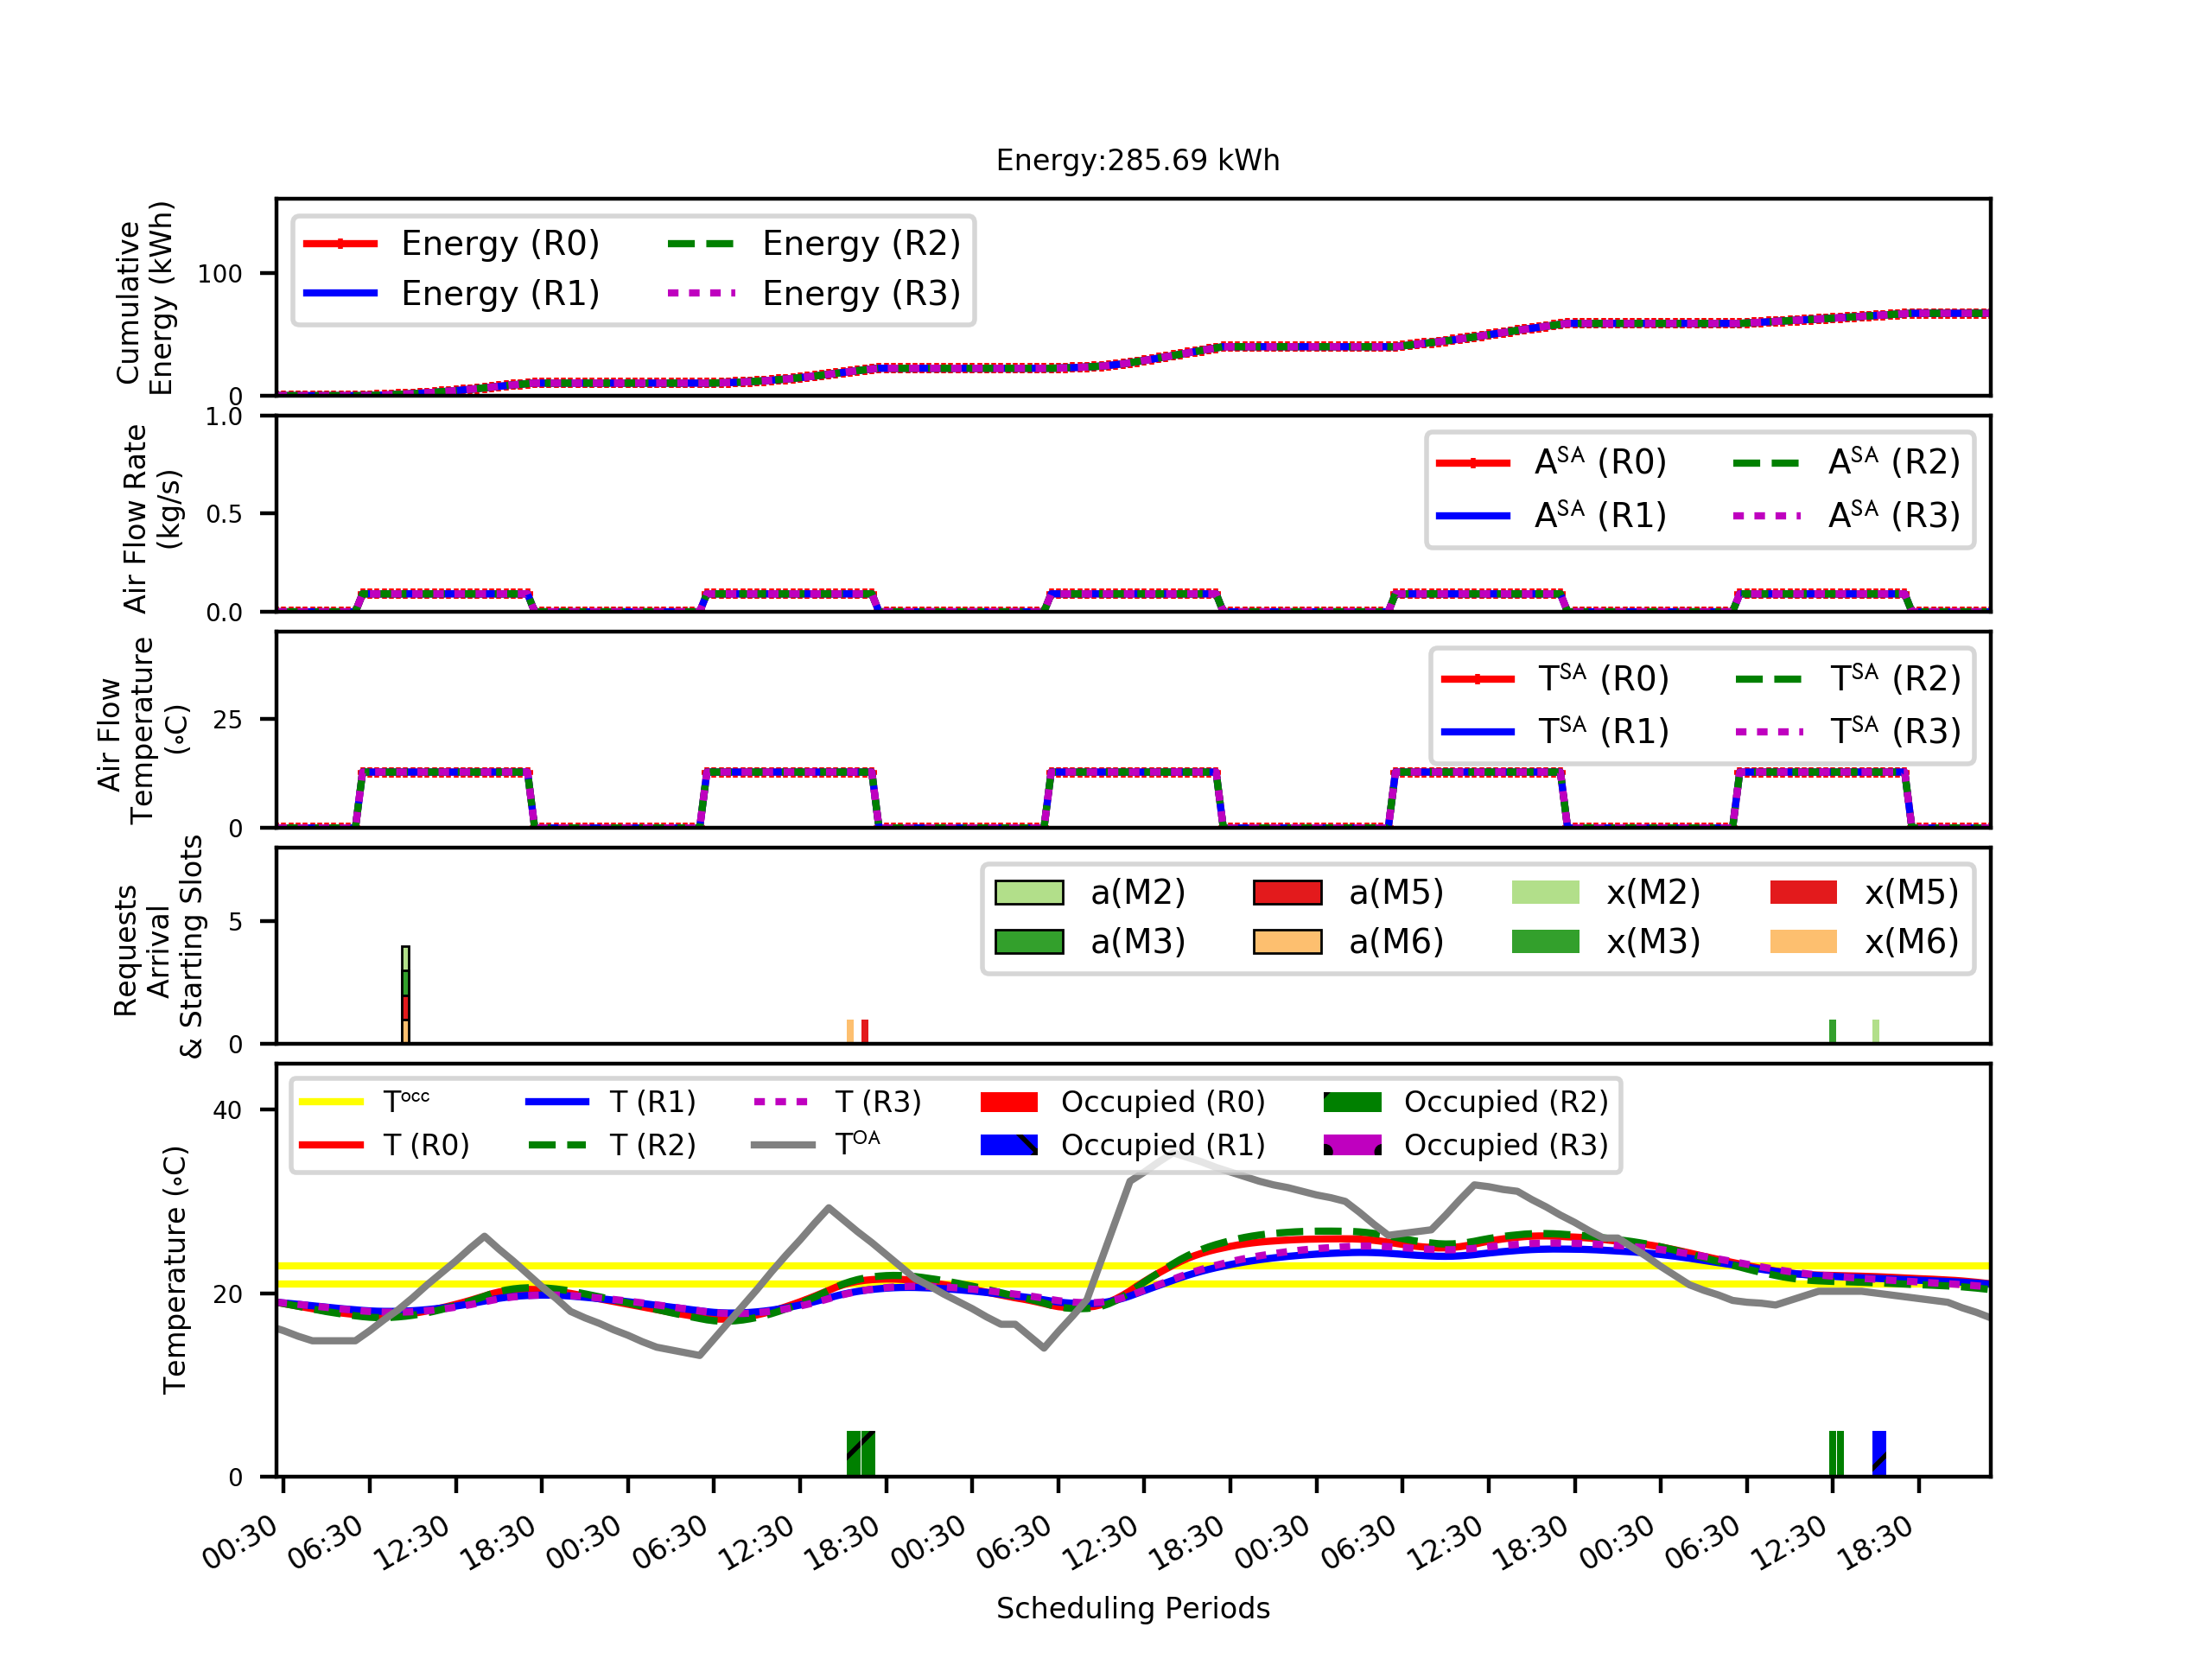
\includegraphics[width=0.9\linewidth]{figs/online_r0.png}
    %\caption{Online Scheduling - Session 1}
    %\label{fig:online_eg1}
%\end{sidewaysfigure}
%
%\begin{sidewaysfigure}[h]
    %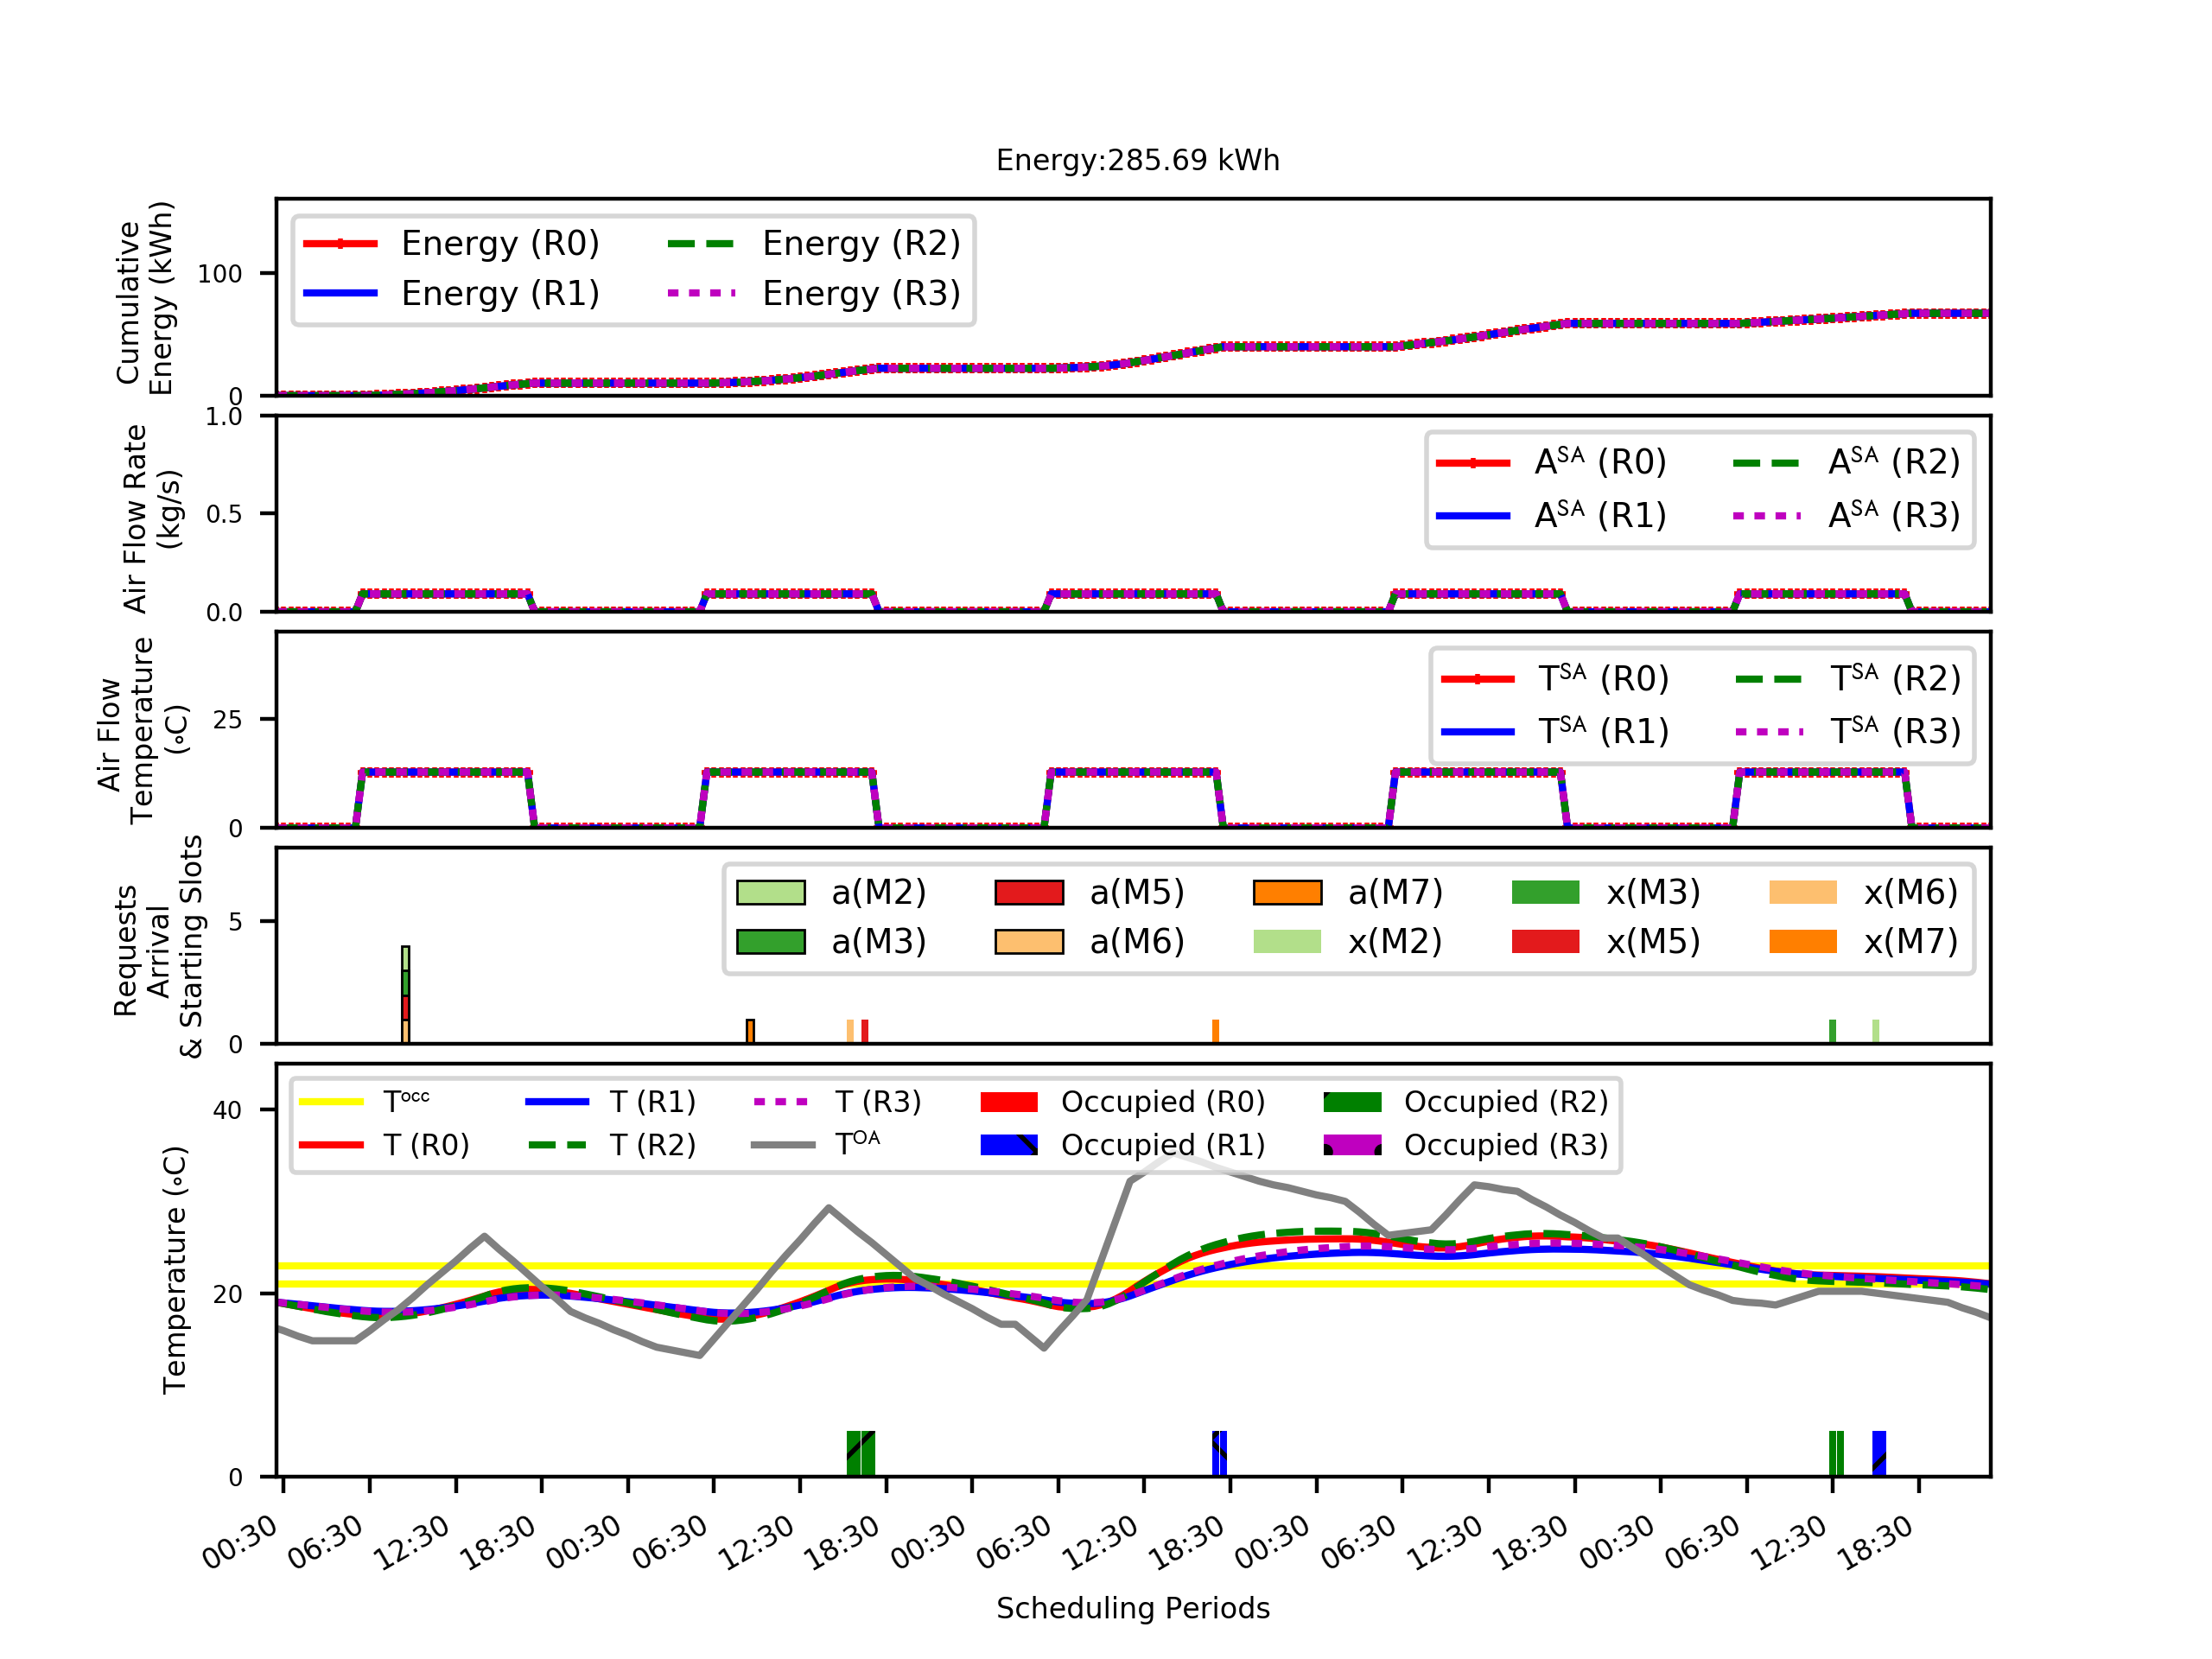
\includegraphics[width=0.9\linewidth]{figs/online_r1.png}
    %\caption{Online Scheduling - Session 2}
    %\label{fig:online_eg2}
%\end{sidewaysfigure}
%
%\begin{sidewaysfigure}[h]
    %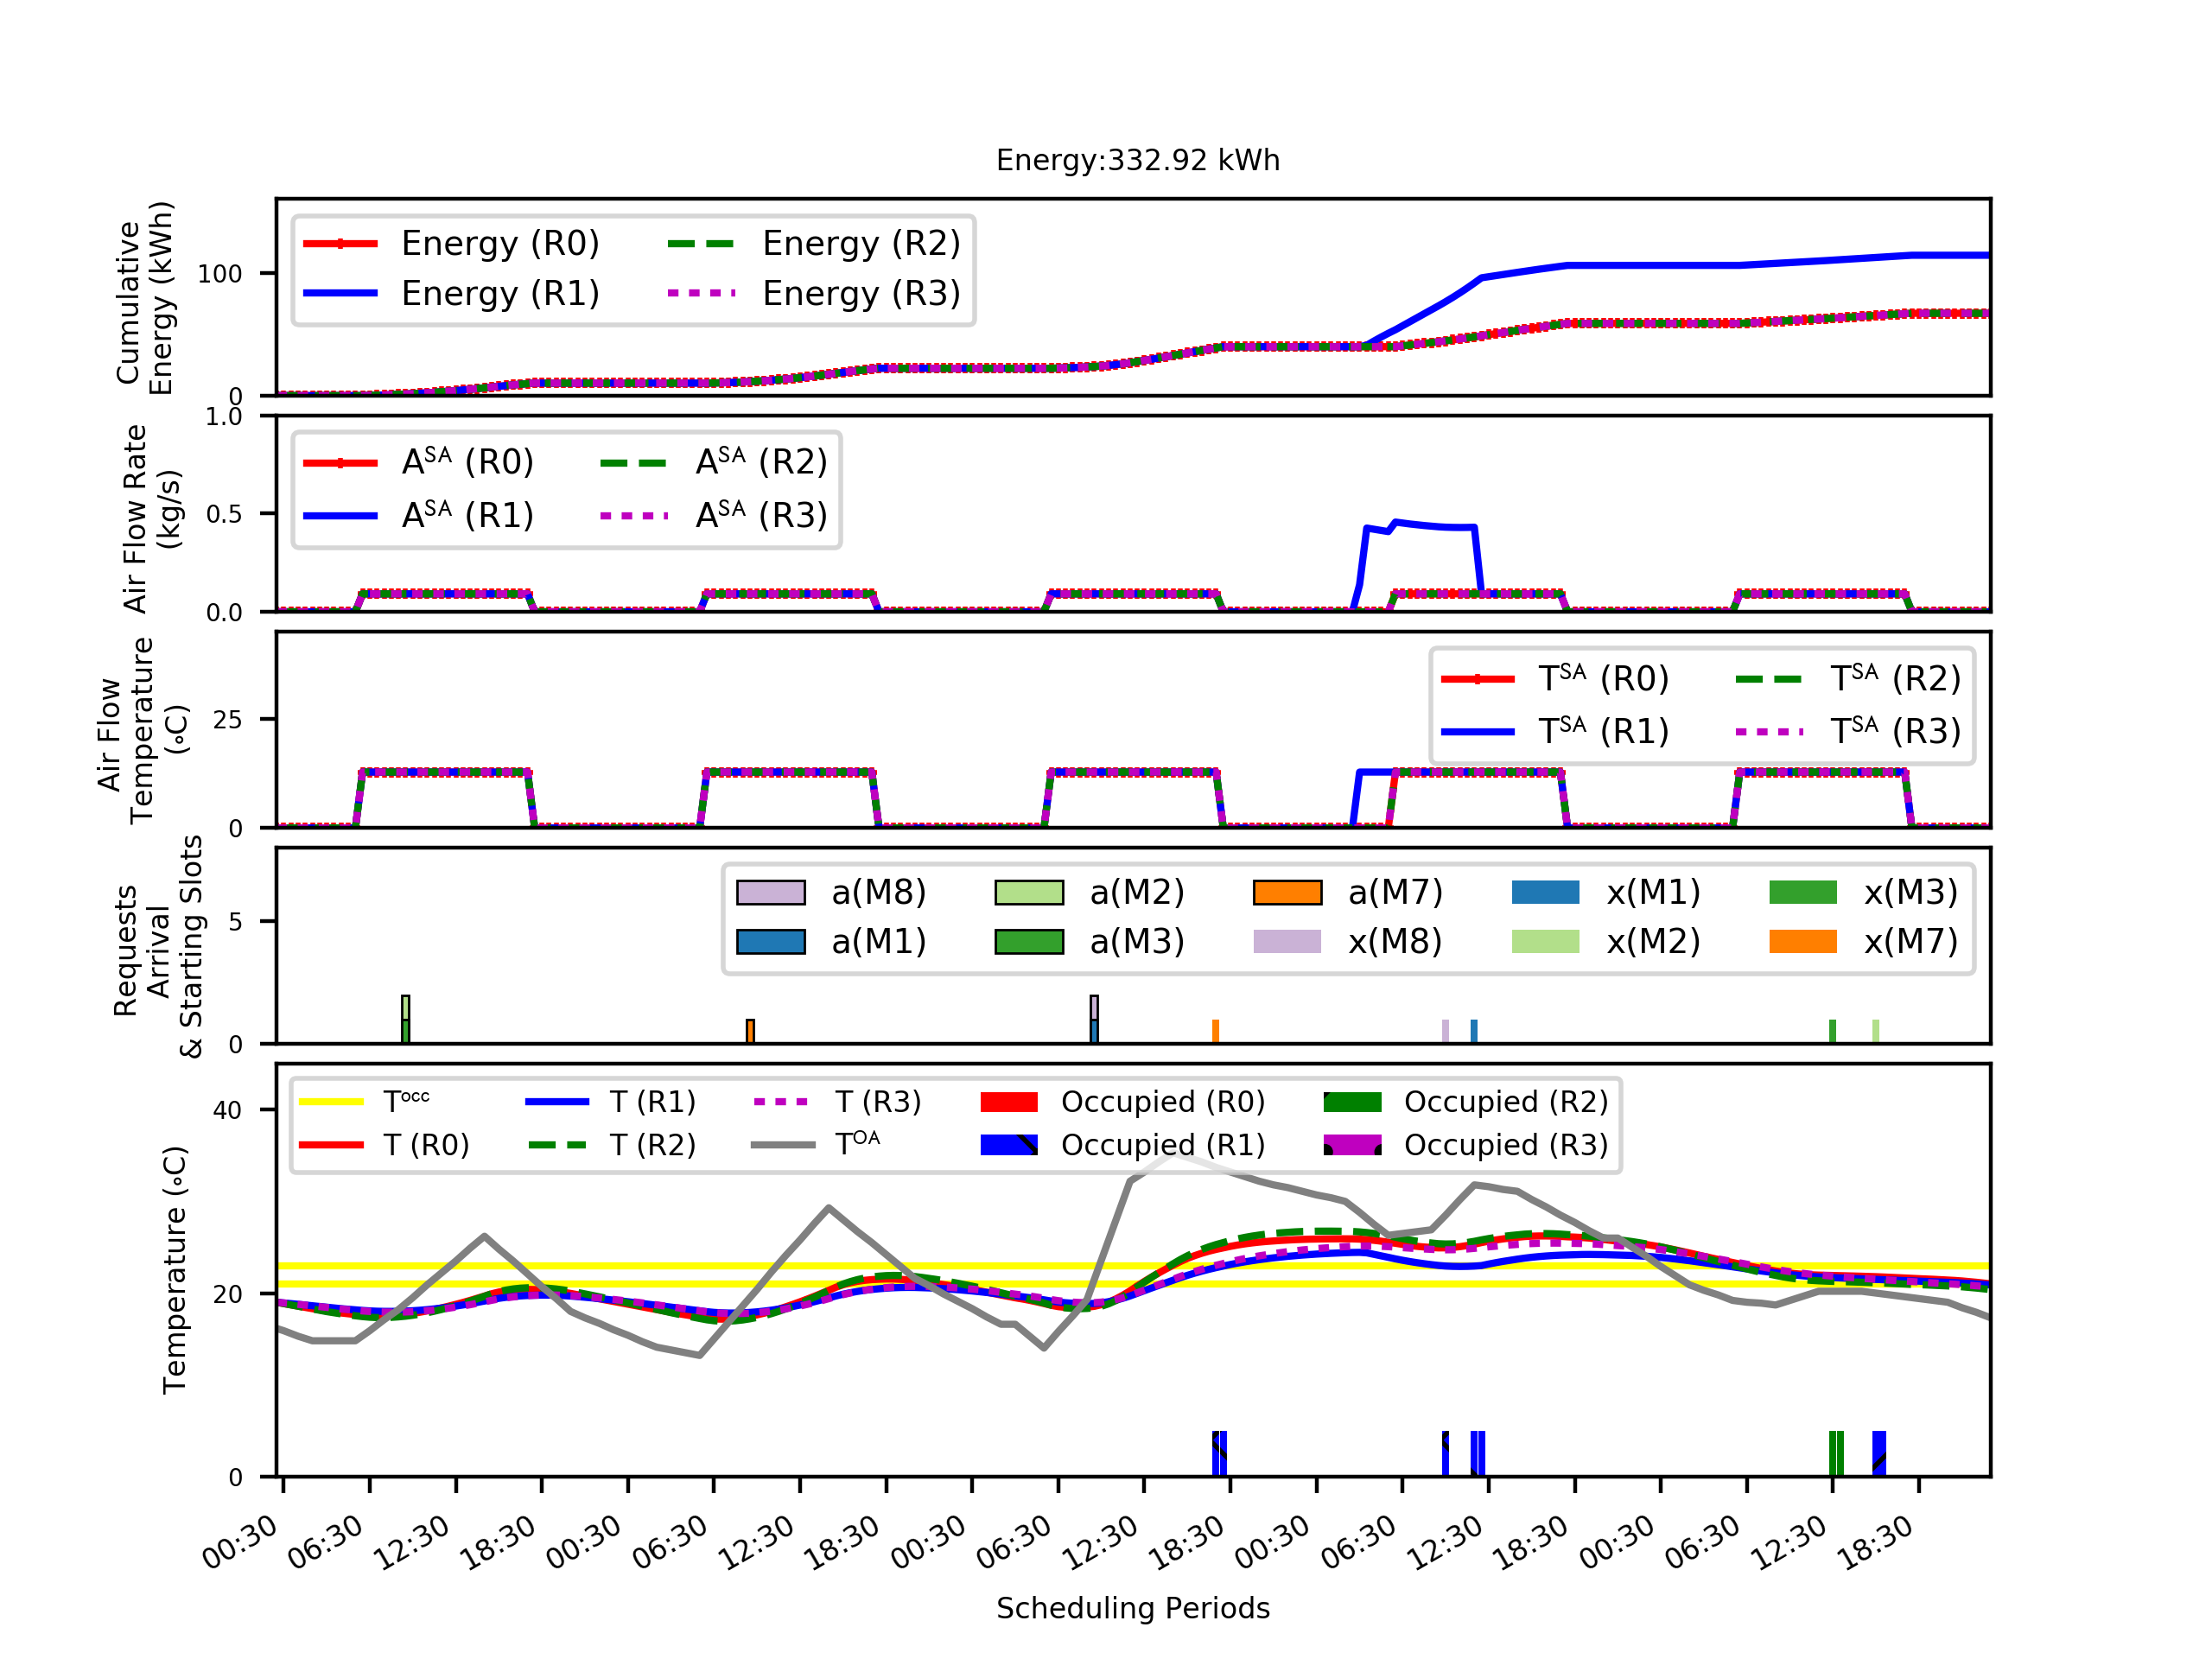
\includegraphics[width=0.9\linewidth]{figs/online_r2.png}
    %\caption{Online Scheduling - Session 3}
    %\label{fig:online_eg3}
%\end{sidewaysfigure}
%
%\begin{sidewaysfigure}[h]
    %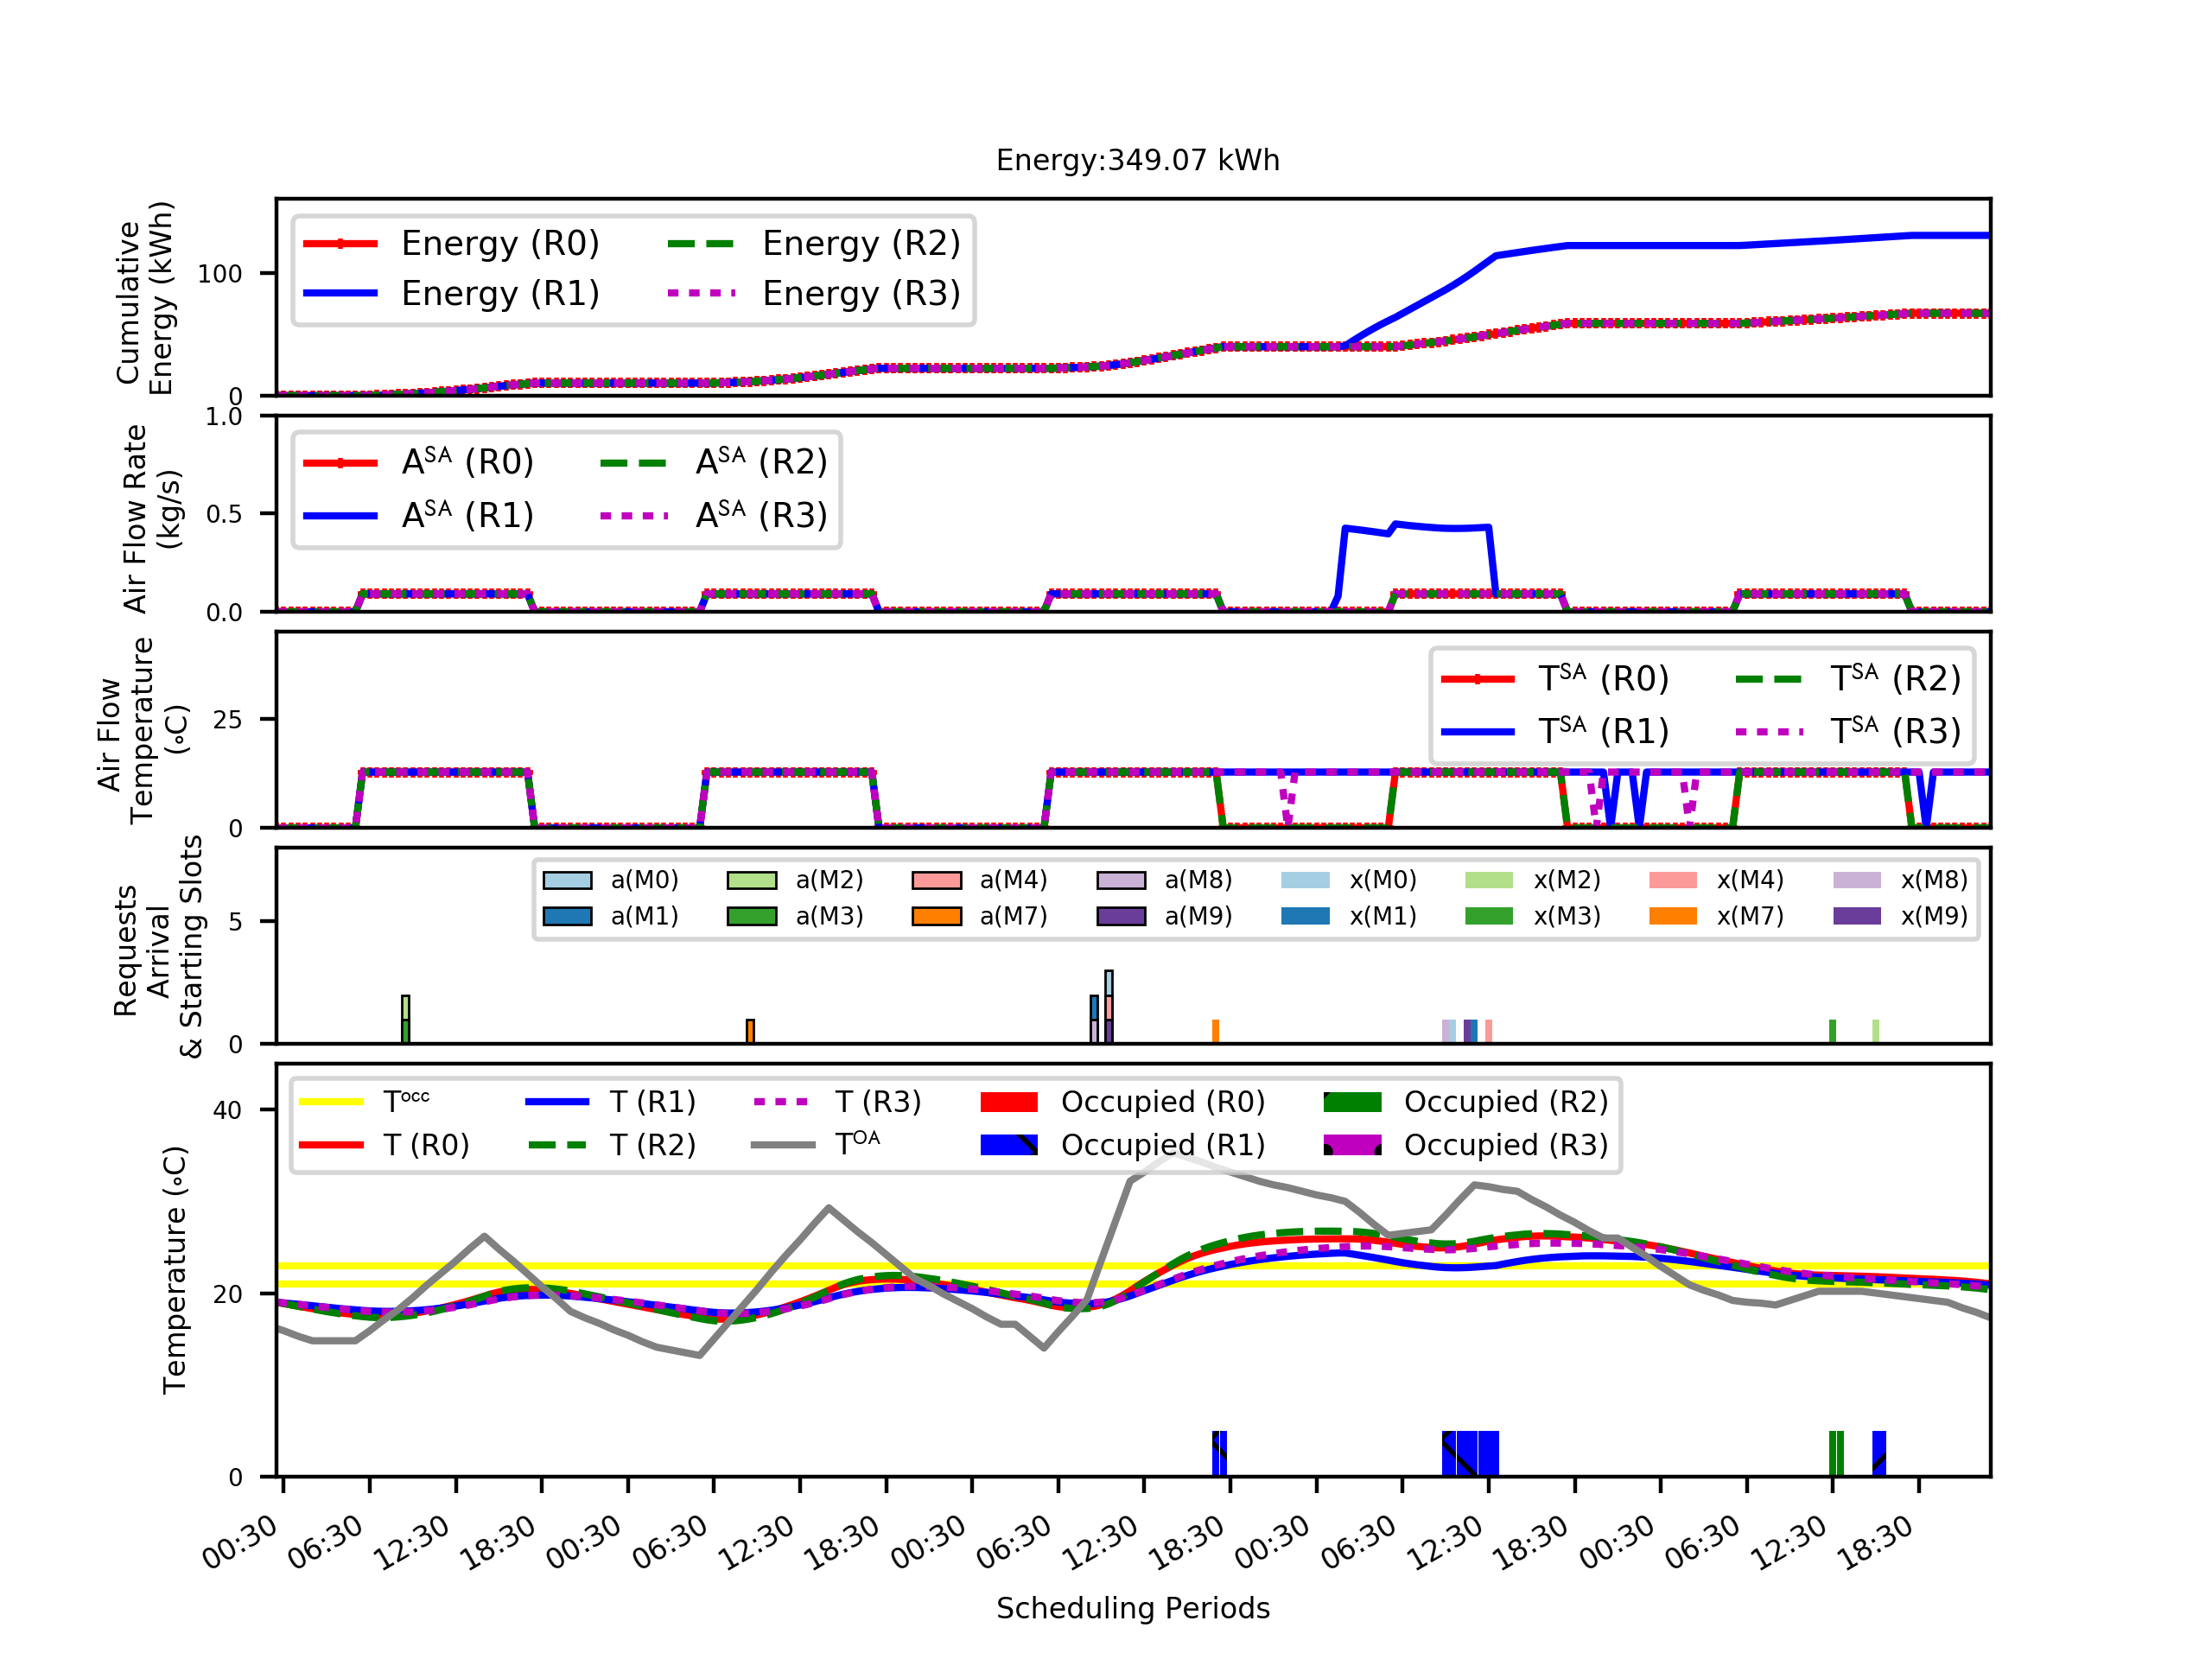
\includegraphics[width=0.9\linewidth]{figs/online_r3.png}
    %\caption{Online Scheduling - Session 4}
    %\label{fig:online_eg4}
%\end{sidewaysfigure}
%
%
%\begin{sidewaysfigure}[ht]
    %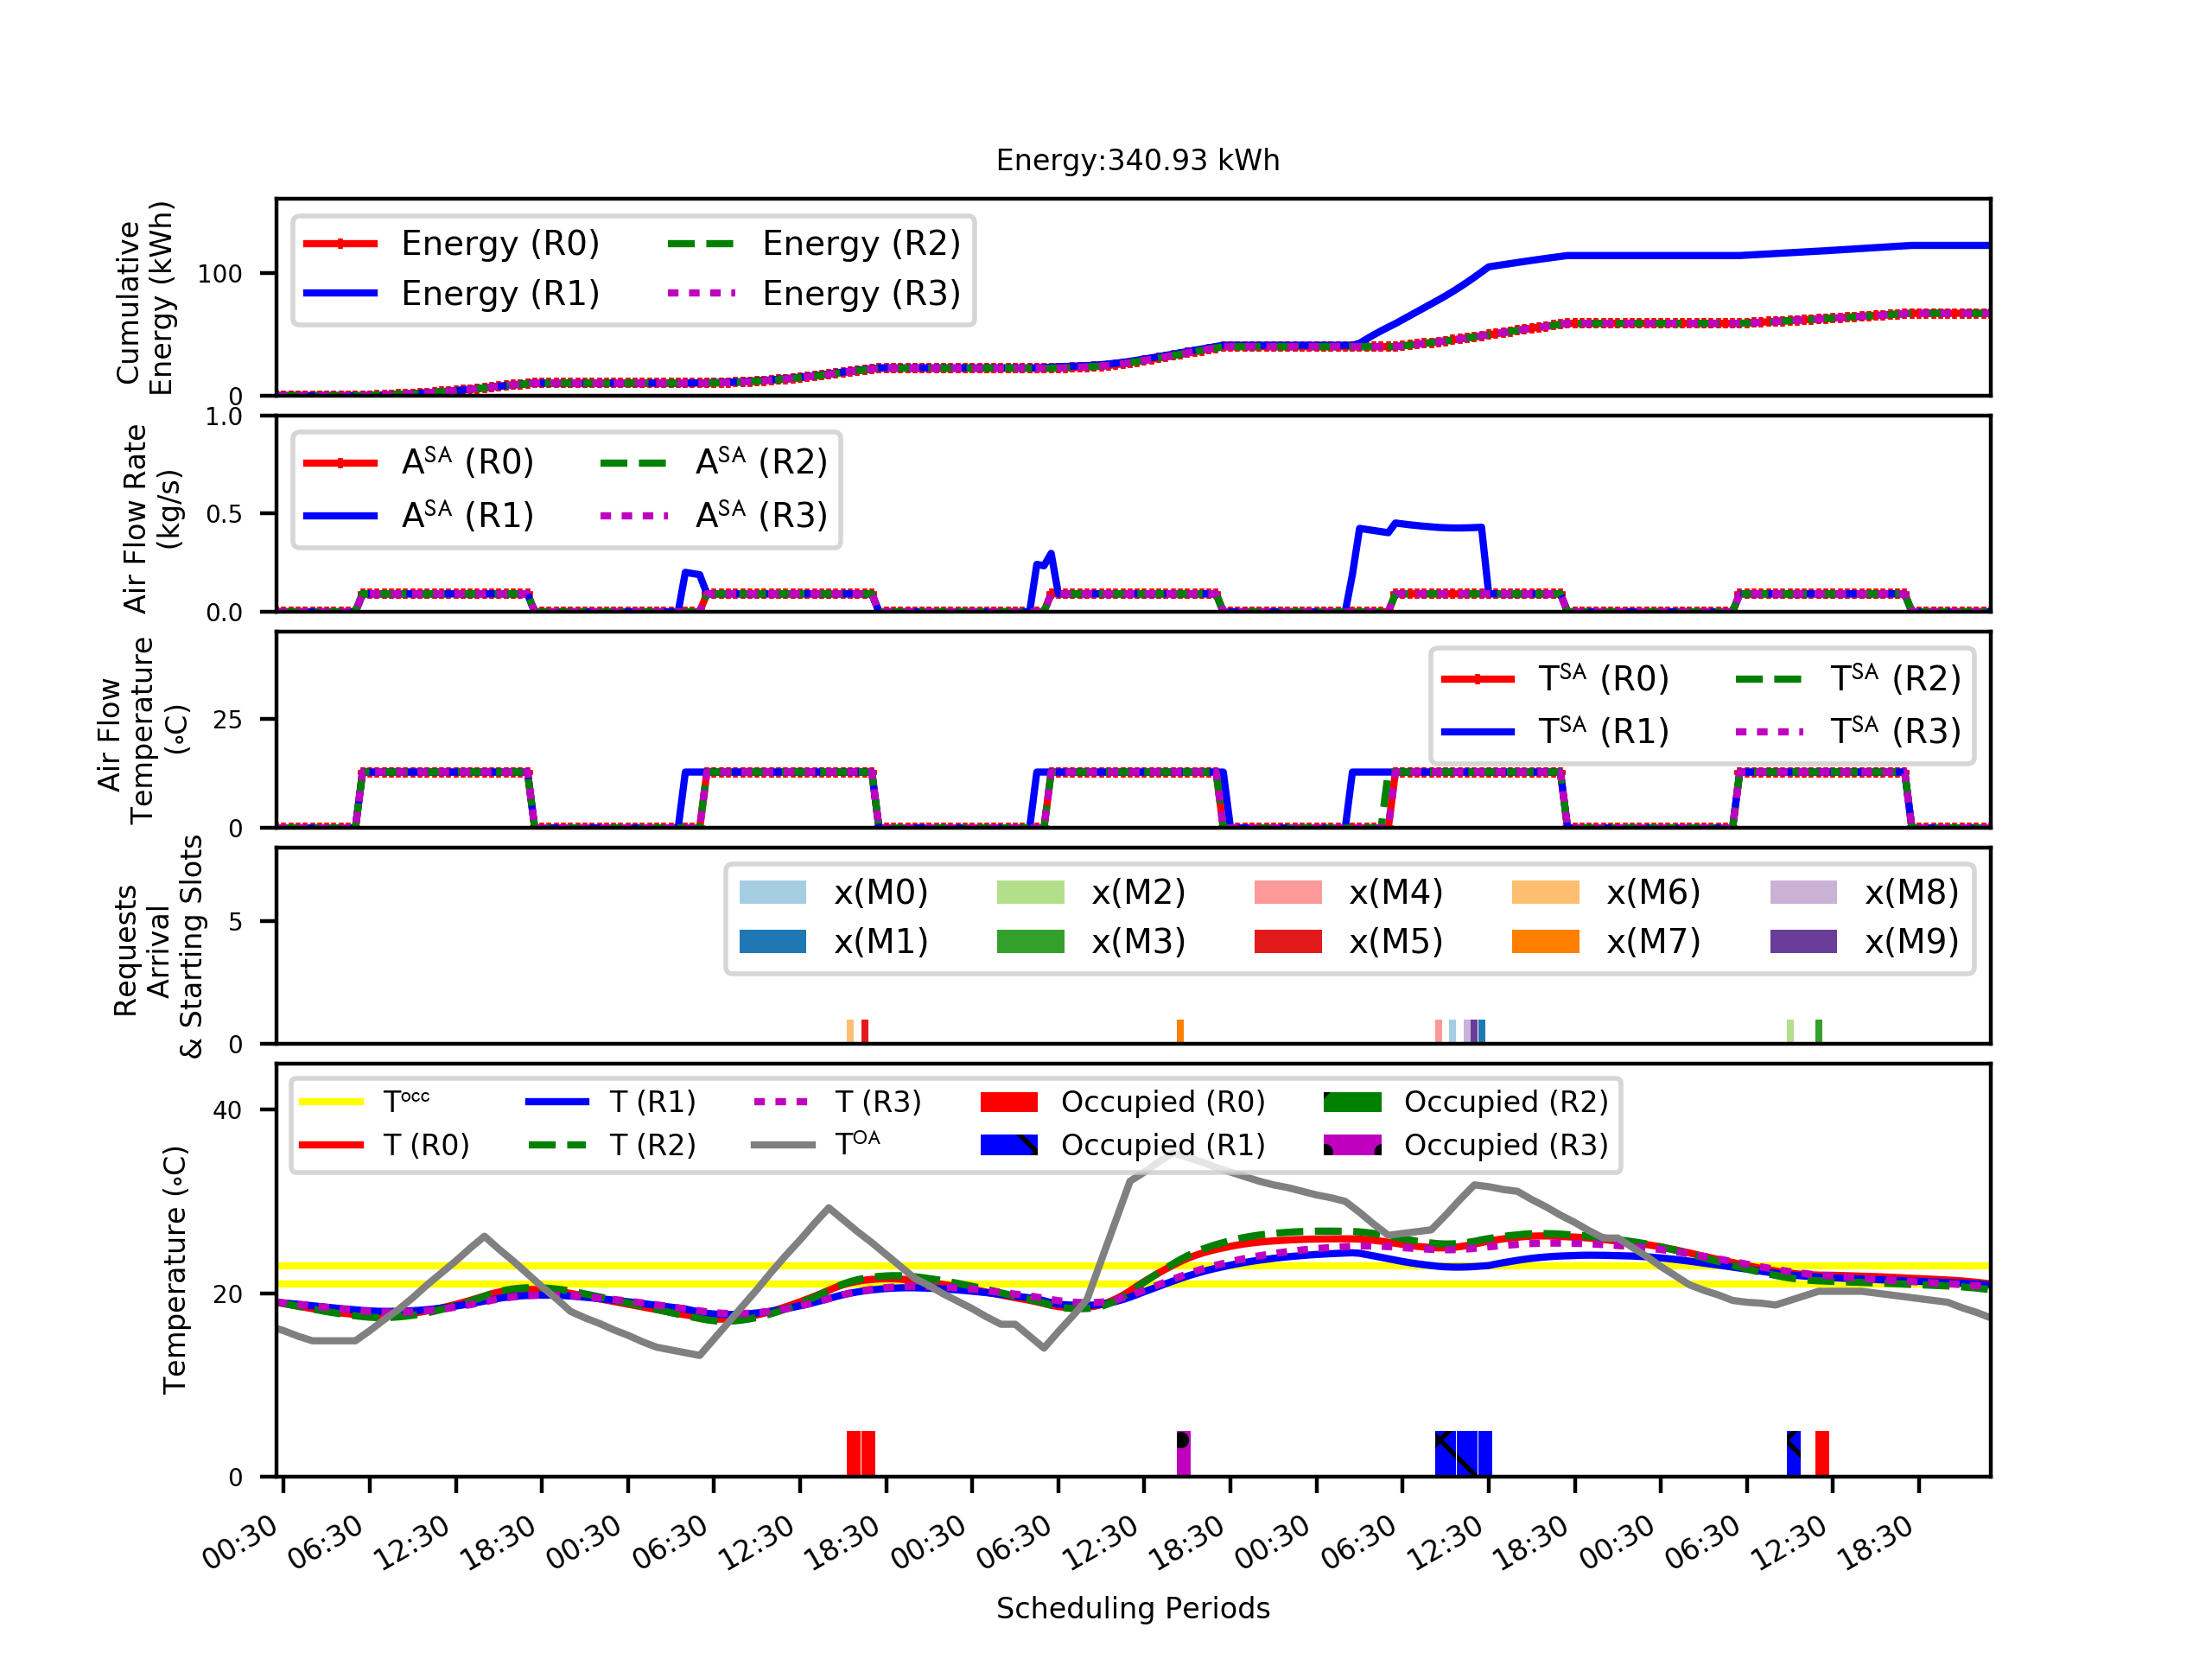
\includegraphics{figs/online_oracle.png}
    %\caption{Offline Scheduling}
    %\label{fig:online_offline}
%\end{sidewaysfigure}


\begin{figure}[t]
\centering
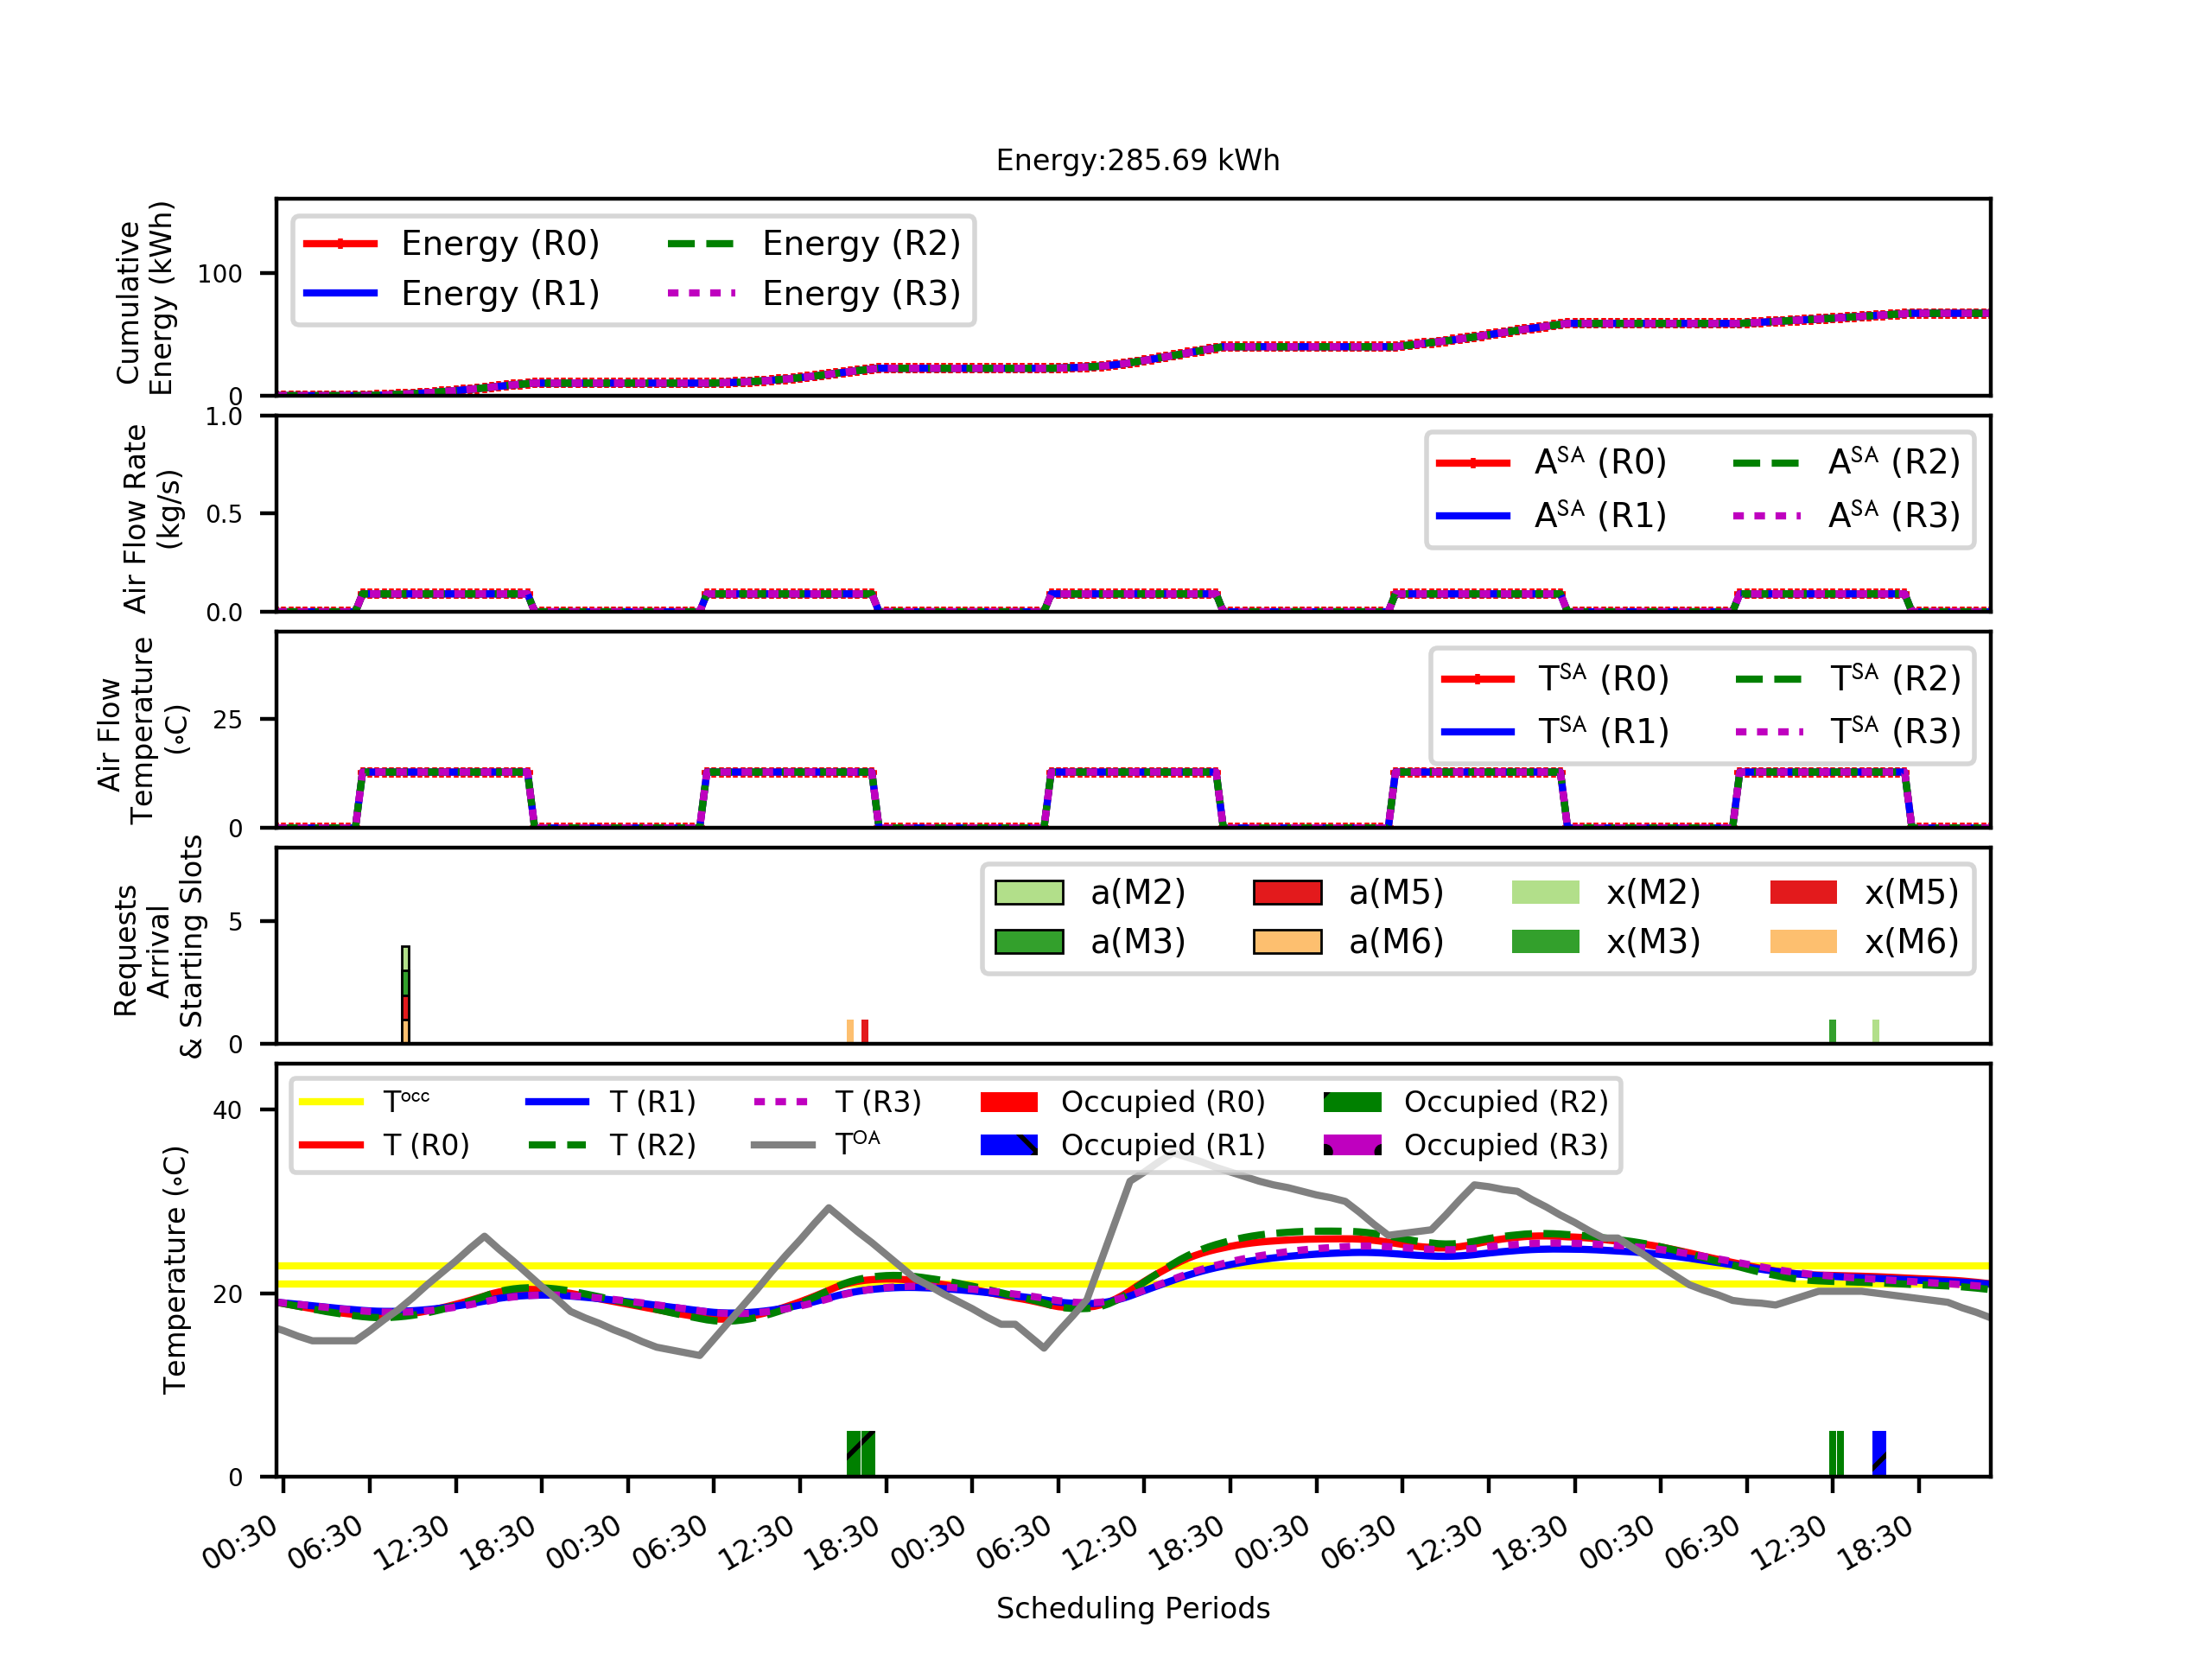
\includegraphics[width=1\linewidth]{figs/online_r0.png}	
\vspace*{-2ex}
\caption{Online scheduling scenario - Session 1}
\label{fig:online_eg1}
\end{figure}

\begin{figure}[t]
\centering
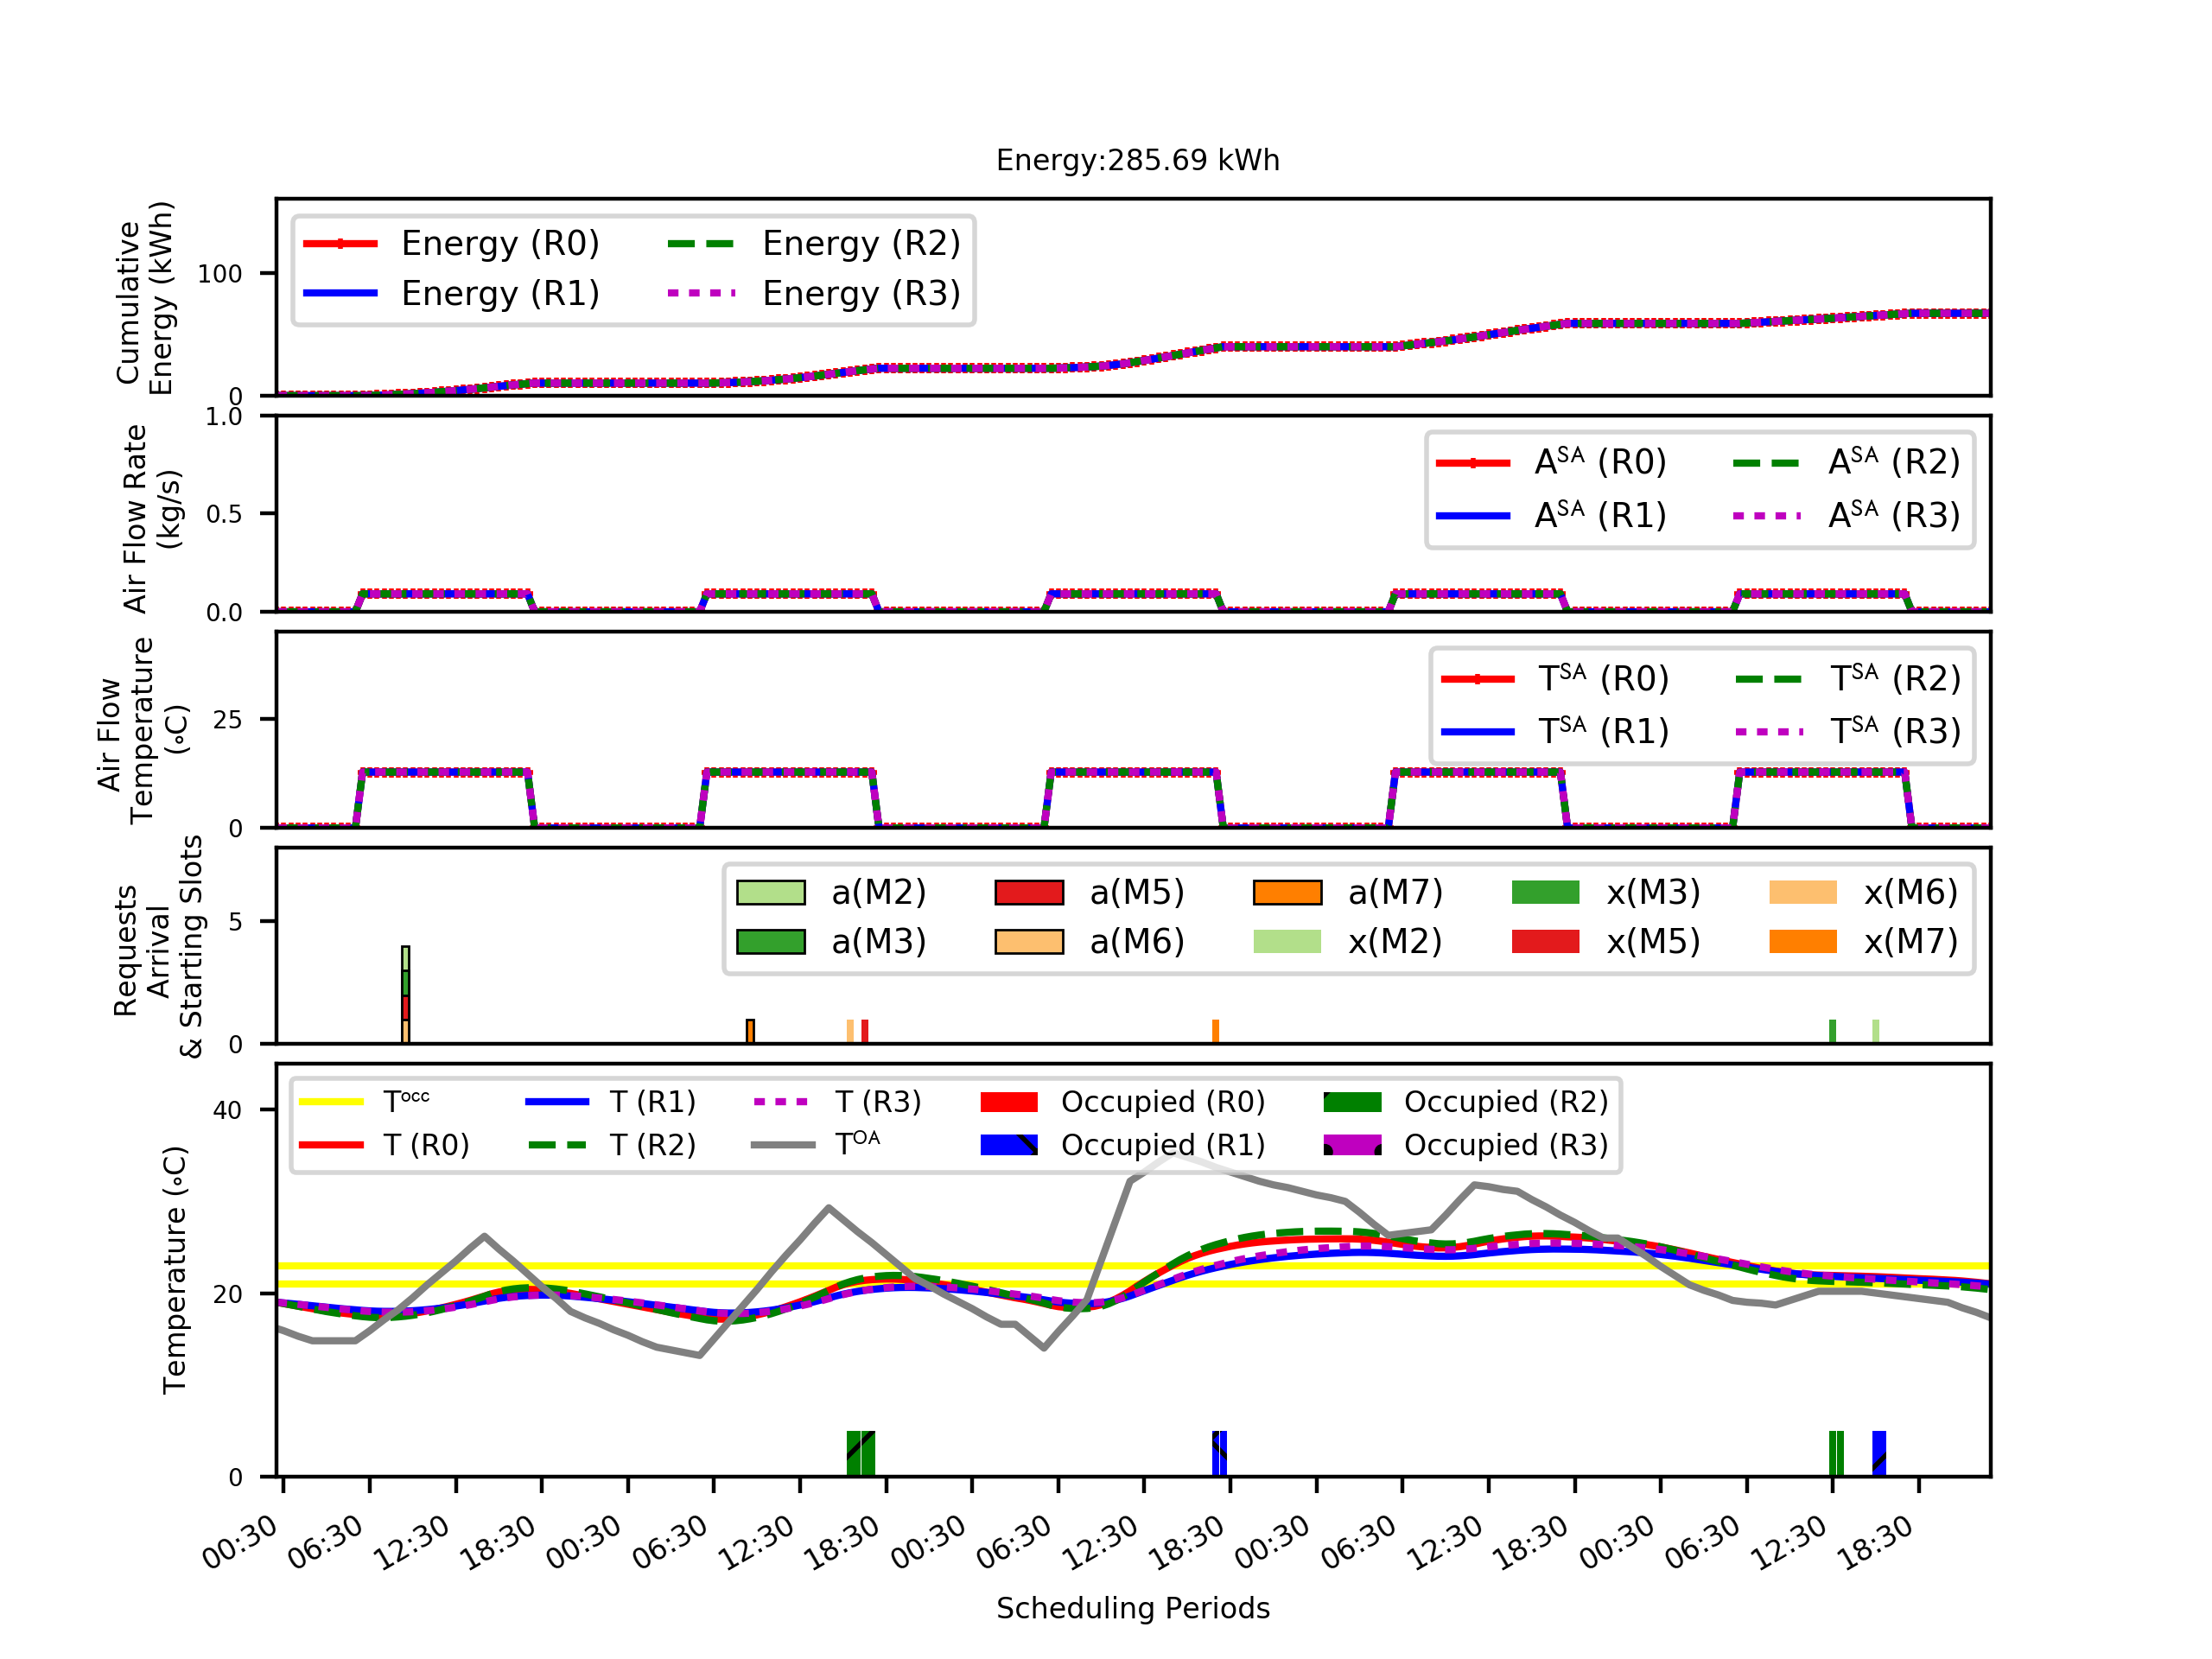
\includegraphics[width=1\linewidth]{figs/online_r1.png}	
\vspace*{-2ex}
\caption{Online scheduling scenario - Session 2}
\label{fig:online_eg2}
\end{figure}


\begin{figure}[t]
\centering
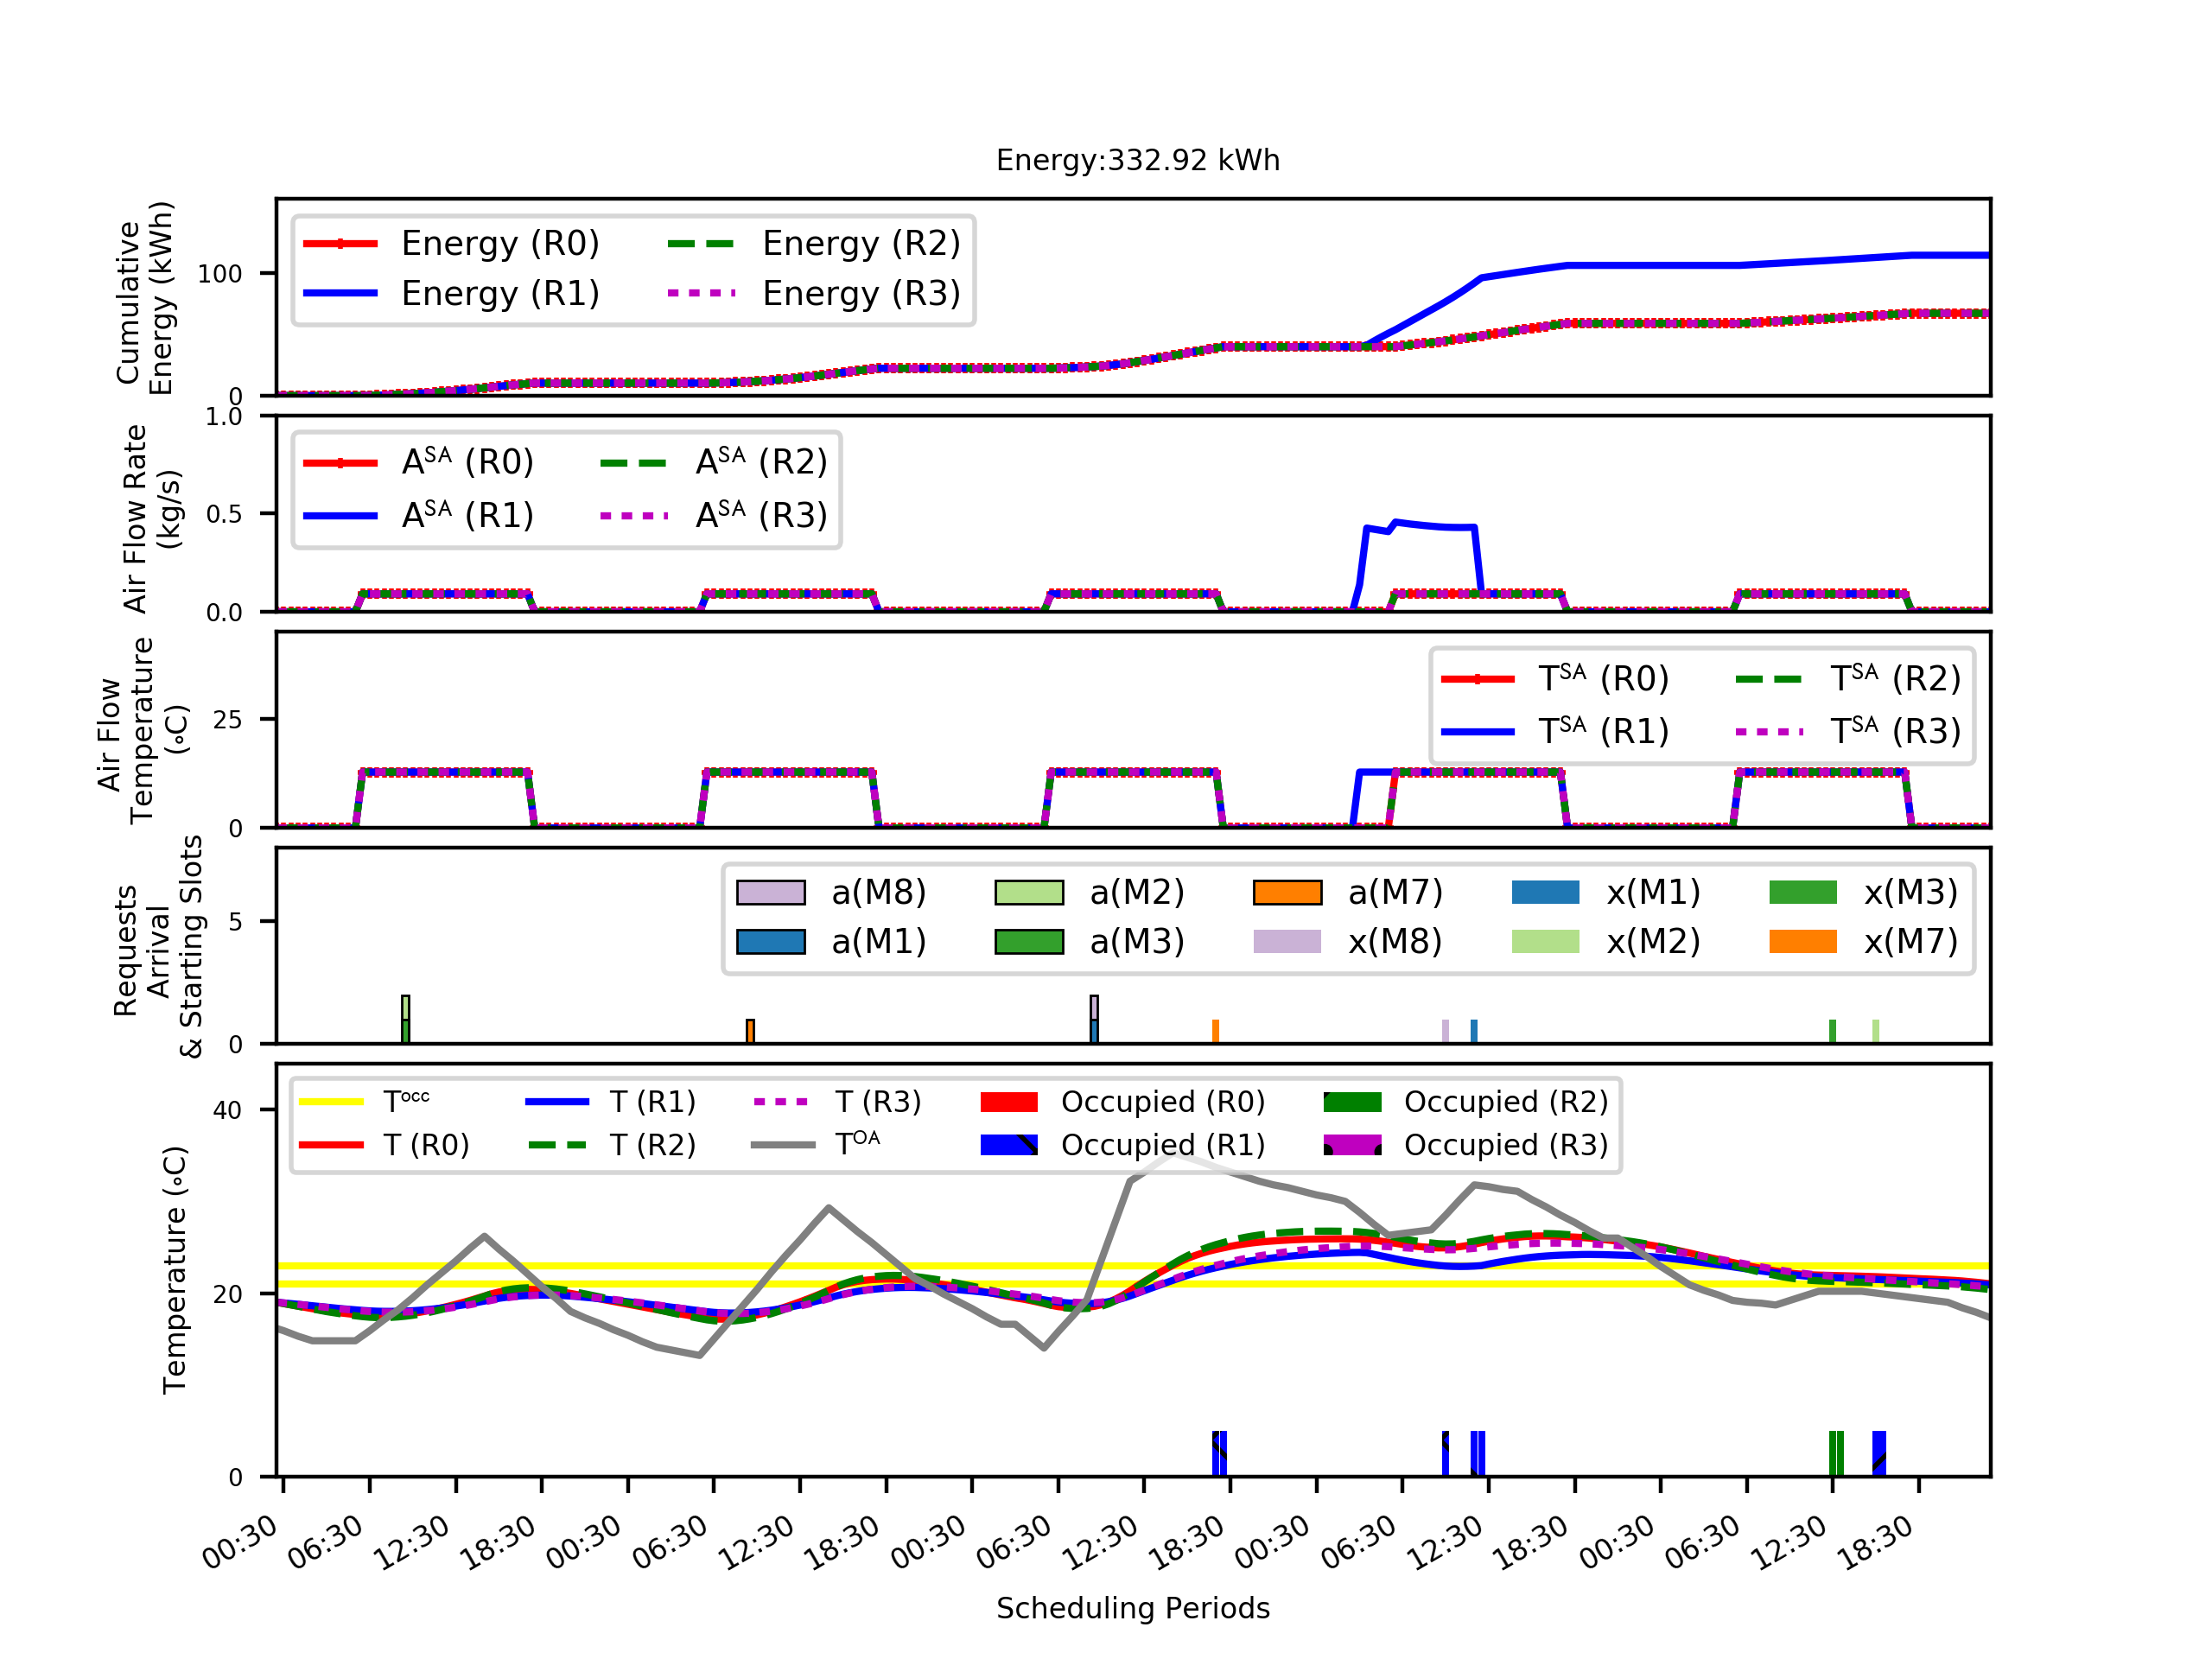
\includegraphics[width=1\linewidth]{figs/online_r2.png}	
\vspace*{-2ex}
\caption{Online scheduling scenario - Session 3}
\label{fig:online_eg3}
\end{figure}

\begin{figure}[t]
\centering
\includegraphics[width=1\linewidth]{figs/online_r3.png}	
\vspace*{-2ex}
\caption{Online scheduling scenario - Session 4}
\label{fig:online_eg4}
\end{figure}

\begin{figure}[t]
\centering
\includegraphics[width=1\linewidth]{figs/online_oracle.png}	
\vspace*{-2ex}
\caption{Offline scheduling scenario}
\label{fig:online_offline}
\end{figure}

Figures \ref{fig:online_eg1}-\ref{fig:online_eg4} show a scenario example of our online HVAC-aware occupancy scheduling. In each figure, from the top, the first sub-graph shows the cumulative energy consumption for each location over the scheduling horizon, the second and third sub-graphs depict the supply air flow rate and air flow temperature for each location, 
%the fourth sub-graph shows the time slots where requests arrive (bar with back stripe) and the time slots where the corresponding meetings start. The arrival time slot and the start time slot for the same meeting are assigned the same color.
the fourth sub-graph illustrates the time slots where requests arrive (bar with black border) and that of meetings start (bar with transparent border). The arrival time slot and the start time slot for the same meeting are assigned with the same color. 
Finally, the fifth sub-graph presents the rooms' temperatures and their occupied status.
For illustration purposes, we plot only the new meeting requests, as well as all ongoing and future activities that have been scheduled prior to the session. All meetings which had occurred prior to current session are removed. 

This scenario consists of 10 meetings $M \in \left\{M0, M1,\ldots, M9\right\}$, which are scheduled in 4 different online sessions. The set of locations is $L = \left\{R0, R1, R2, R3\right\}$. We set 5 minutes for the LNS runtime limit and 8.5 seconds for the MIP runtime during each repair step. For simplicity, we present the graphs in a finite horizon consisting of 240 steps, and use the same set of outdoor temperature and solar gain for each session.

Figure \ref{fig:online_eg1} illustrates the first online session. This session consists of 4 meeting requests $m \in \left\{M2, M3, M5, M6\right\}$. M2 and M3 are one hour meetings which need to be held 4 days after the meeting requests are made, and can be scheduled within any consecutive slots between 09:00 to 18:30. M5 and M6 have similar properties as M2 and M3, except that the meetings are to be held the next day after the meeting requests are made. In this scenario, M2 and M3 are scheduled at 15:30-16:30 in R1 and 12:30 to 13:30 in R2 respectively, whilst M5 an M6 are being scheduled back-to-back in R2 between 16:00 to 18:00.
The scheduler manages to find optimal times and locations that rely solely on minimum HVAC ventilation and the outdoor temperature to achieve a comfort temperature between 21$^\circ$C-23$^\circ$C.

Figure \ref{fig:online_eg2} shows the second online session with only one meeting request $M \in \left\{M7\right\}$. M7 is a 1-hour meeting which can be held between 09:00 to 18:30 on the next day after the request is made. We note that this meeting is being assigned to R1 on a late afternoon from 17:30 to 18:30. At that time, R1's room temperature is already within the occupied temperature bounds. The HVAC control is optimised, and hence does not need to be changed for all pre-scheduled meetings  $M \in \left\{M2, M3, M5, M6\right\}$ and the new meeting, M7.

Figure \ref{fig:online_eg3} depicts the third online session with 2 new meeting requests $M \in \left\{M1, M8\right\}$ and 3 pre-scheduled meetings $M \in \left\{M2, M3, M7\right\}$. M1 is a 1-hour meeting whilst M8 is a 30-minute meeting. Both can be scheduled between 09:00 to 18:30 on the next day after the requests are made. Note that the requests are made on the hottest day of the week, and the meetings are to be held on the next day when the outdoor temperature is still high. In this scenario, M8 is scheduled at 09:30 to 10:00 whilst M1 is scheduled between 11:30 to 12:30. The scheduler picks R1 as the meetings' location, as its room temperature is the closest to the occupied comfort bound (hence less energy is required for space cooling). The HVAC control strategy for R1 is revised such that the HVAC is activated at 04:00 to push in 0.14 \mbox{kg/s} to 0.45 \mbox{kg/s} of cold air into the room. This cooling operation continues up until 12:00 noon, right before M1 finishes. %No additional is cooling required for M1 which is held subsequently between 

Figure \ref{fig:online_eg4} shows the fourth online session with 3 new meetings requests $M \in \left\{M0, M4, M9\right\}$ and 5 pre-scheduled meetings $M \in \left\{M1, M2, M3, M7, M8\right\}$. $M0$ and $M4$ are 1-hour meeting whilst $M9$ is a 30-minutes meeting. All new meetings can be scheduled between 09:00 to 15:30 on the next day after the requests are made. In this scenario, $M0$ and $M9$ have been slotted in between $M8$ and $M1$ whilst $M4$ is scheduled right after $M1$ to leverage on thermal inertia. The HVAC control strategy for R1 is revised again by activating standby-mode and pushing in 0.08 \mbox{kg/s} to 0.45 \mbox{kg/s} of cold air into the room from 02:00.

Using our online algorithm, the total energy consumption for these 10 meetings is 349.07 kWh. We compare this solution quality with that of the offline approach used in Chapter \ref{cha:lns}. For the offline approach, we set LNS runtime limit to 2 hours and MIP runtime limit to 15 seconds. Figure \ref{fig:online_offline} presents the result of the offline approach. In this scenario, the offline approach achieves merely 8 kWh of energy savings compare to the online approach. 
Given that the schedules for meetings $M \in \left\{M0, M1, M4, M8, M9\right\}$ are known upfront in the offline approach, it is able to activate standby-mode for room R1 on 3 consecutive early mornings. This helps to bring down the room temperature to a state that lesser cooling load is required, and leads to 340.93 kWh of energy consumption. 
If we compare it with Figure \ref{fig:online_eg4}, albeit lacking of prior knowledge on future requests, the online approach, however, is capable of revising the HVAC control strategy to activate standby-mode on an earlier hour and slot in new requests in the room that have been pre-scheduled with meetings. 
It is worth noting that both offline and online approaches are capable of generating similar schedules that do not incur additional energy cost for $M \in \left\{M2, M3, M5, M6, M7\right\}$. 
%requests for $M \in \left\{M2, M3, M5, M6, M7\right\}$ arrive at least a day prior to their start time, and these meetings have a flexible time window of at least 18 starting slots. In this case, both offline and online approaches are capable of generating similar schedules that does not incur additional energy cost. 

The strengths of this online model are its capability to handle dynamic request and feedback to the user in a timely manner, its ability to re-optimise the HVAC control each time it considers new requests and the combinations of both that make this mechanism computationally efficient and practical for real-world trial.


\section{Experiments} \label{sec:online:experiments}
\subsection{Problem Sets}

We analyze our contributions using 9 problem sets with increasing numbers of activities (meetings) and locations (meeting rooms). The problem sets are labeled 10M-4R, 20M-20R, 50M-20R, 100M-20R, 200M-20R, 50M-50R, 100M-50R, 200M-50R, and 500M-50R, where $x$M-$y$R consists of problem instances with $x$ meetings and $y$ rooms. Each set contains 80 problem instances, giving a total of 720 instances, obtained as follows. 

We start from a set of real data from 32,065 unique meetings in a USC library collected by \cite{kwak2013tesla}. Each meeting request in this original data set includes the request arrival time, start time, duration, specified room and number of attendees. We first derive a probability distribution on meeting start times from this data set. To obtain a set of requests, we sample $x$ meetings from this distribution. We then create different instances with that set of requests by varying the time flexibility and the request-to-start time gap of the requests. The time flexibility of a request $m$ is its number $|K_m|\in \{1,2,4,8,32\}$ of permissible start time steps. The request-to-start time gap denotes the duration $\{\mbox{10 minutes, 1 hour, 4 hours, 24 hours}\}$ between the request's arrival time ${\bm a}_m$ and its first possible start time step. 

In all problem sets, we keep the meeting duration and number of attendees identical to that of the original meeting request from the USC data. The duration ${\bf d}_m$ of meetings ranges from 1 to 4 time steps (30 minutes to 2 hours). All meetings have between 2 and 30 attendees. The meetings must be scheduled over a period of 5 summer days. The available rooms are located in 5 buildings with a $1\times4$ zone layout (as in Chapter \ref{cha:lns}). We assume that the occupant is fully flexible in terms of location, that is, that the meeting can be allocated to any room. 
%The available rooms are located in 5 buildings and differ by their thermal resistance and capacitance (as in chapter \ref{cha:lns}). We use a $1\times4$ zone layout where each zone has the same thermal resistance and capacitance as its neighboring zones. Moreover, all rooms have the same geometric area of $6\times10\times3$ m$^3$ with a window surface area of $4\times2$ m$^2$ and a capacity of 30 people. The solar gain ranges from $50$ to $350$~W/m$^2$ during the day. 
All our experiments were run on a cluster consisting of a 2 $\times$ AMD 6-Core Opteron 4334, 3.1GHz with 64GB memory. 


\subsection{Online vs. Offline Scheduling}

We start by comparing the solution quality of our online approach with that of the offline approach using the above problem sets.
%a larger set of problems with different constrainedness. 
In the online approach, the scheduler runs LNS for 5 minutes in each session, with a MIP runtime limit of 8.5 seconds in each iteration. In the offline approach, the entire set of requests to schedule is given, and we compute the final schedule; The scheduler runs LNS for 2 hours, with a MIP runtime limit of 15 seconds in each iteration. To identify how much more improvement can be obtained, we warm start the offline schedule with the best online solution found (over all the possible request-to-start time gaps).

\begin{figure}
\centering
\begin{tabular}{c}
\includegraphics[width=.8\linewidth]{figs/perc_excess_energy_oracle_def_compile_mtd.png}
\end{tabular}
\caption{Online vs. offline scheduling}
\label{fig:oracle_vs}
\end{figure}

%0   1   1086.89   1054.6   32.29   3.06182438839
%0   2   1086.89   1046.84   40.05   3.82579954912
%0   3   1086.89   1034.17   52.72   5.09780790392
%0   4   1086.89   938.83   148.06   15.7706933098
%5   6   4934.22   4928.49   5.73   0.116262790429
%5   7   4934.22   4871.77   62.45   1.28187496536
%5   8   4934.22   4718.09   216.13   4.58087912693
%5   9   4934.22   4620.63   313.59   6.78673687354
%10   11   5197.34   5160.12   37.22   0.721301055014
%10   12   5197.34   5026.82   170.52   3.39220421658
%10   13   5197.34   4914.0   283.34   5.76597476597
%10   14   5197.34   4692.71   504.63   10.7534878567
%15   16   5497.76   5443.64   54.12   0.994187712633
%15   17   5497.76   5248.63   249.13   4.74657196259
%15   18   5497.76   5066.95   430.81   8.50235348681
%15   19   5497.76   4733.29   764.47   16.1509225084
%20   21   6258.15   6106.18   151.97   2.48879004549
%20   22   6258.15   5795.47   462.68   7.98347674994
%20   23   6258.15   5503.81   754.34   13.7057783608
%20   24   6258.15   4913.25   1344.9   27.3729201649
%25   26   12202.22   12150.95   51.27   0.421942317267
%25   27   12202.22   12033.22   169.0   1.40444536043
%25   28   12202.22   11927.74   274.48   2.30119033446
%25   29   12202.22   11629.3   572.92   4.92652180269
%30   31   12518.28   12475.19   43.09   0.345405560957
%30   32   12518.28   12268.26   250.02   2.03794181082
%30   33   12518.28   12082.84   435.44   3.6037885133
%30   34   12518.28   11774.85   743.43   6.31371100269
%35   36   13306.09   13160.57   145.52   1.10572718355
%35   37   13306.09   12858.53   447.56   3.48064669912
%35   38   13306.09   12563.96   742.13   5.90681600387
%35   39   13306.09   11919.53   1386.56   11.6326734359
%40   41   15801.01   15536.29   264.72   1.70388168604
%40   42   15801.01   14740.27   1060.74   7.19620468282
%40   43   15801.01   13782.34   2018.67   14.6467871203
%40   44   15801.01   12279.7   3521.31   28.6758634169
\begin{figure}[h]
\centering
\begin{tabular}{c}
  \includegraphics[width=0.8\linewidth]{figs/energy_tf_def_mtd_perc.png} 
\end{tabular}
\caption{Time flexibility vs. energy savings}
\label{fig:online_tf}
\end{figure}

The difference of solution quality, that is the excess consumption of the online scheduling as a percentage of the offline scheduling consumption, is shown in Fig.~\ref{fig:oracle_vs}. The results show that the offline solutions are merely 1\% better than the online solutions for tightly constrained problems (such as 200M-20R, 500M-50R). Note that in the online approach, at most 20 requests arrive in each online session and a maximum of 4 rooms are destroyed, thus the sub-problems formed are small enough for MIP to solve them to (near) optimality. The offline approach has many more meetings to deal with, but on the other hand, as problems become more constrained, it has more room to optimise than the greedy online approach. Altogether, even with a simple greedy approach, our online algorithm is able to perform effectively without prior knowledge of future requests. 

We also investigate the impact of energy savings with different time flexibility and request-to-start time gap. 
The amount of energy savings from meetings with 2 slots to 32 slots of permissible start time, as a percentage of the energy consumption incurred by meetings with strictly 1 permissible start time, is shown in Figure \ref{fig:online_tf}. We note that meetings with higher time flexibility achieve more energy savings than that of with lower time flexibility. The total savings can go up to 2.5\% with 2 flexible starting slots, and 28.7\% with 32 flexible starting slots. We also observe that, while a longer request-to-start time gap can lead to some savings on energy consumption, the influence of request-to-start time gap is relatively obvious when it comes to generating feasible solutions, which is covered in the next section.


\begin{figure}
\centering
\begin{tabular}{c}
  \includegraphics[width=0.8\linewidth]{figs/feasibility_tf_def_mtd.png} \\
(a) Time flexibility \\[6pt]
  \includegraphics[width=0.8\linewidth]{figs/feasibility_cvs_def_mtd.png} \\
(b) Request-to-Start time gap \\[6pt]
\end{tabular}
\caption{Solution feasibility}
\label{fig:def_feas}
\end{figure}


\subsection{Model Feasibility}

%From the experiments, we notice two important properties that constraint the solution feasibility of our online solution. These properties are: (1) time flexibility, i.e. the number of possible starting slot for a meeting; and (2) request-to-start time gap, i.e the time gap between the request arrival time and its start time. 
From the experiments, we notice that time flexibility and request-to-start time gap constrain the solution feasibility of our online solution. In this section, we investigate further how different settings of these properties impact the feasibility performance of our model. Figure \ref{fig:def_feas} depicts the percentage of problem instances which are solvable, given different time flexibility and request-to-start time gap. 

In terms of time flexibility, Figure \ref{fig:def_feas}(a) shows that the number of problem instances which is solvable  does not vary a lot for problems with less than 4 possible starting slots. However, time flexibility impacts loosely constrained problems such as 10M-4R and tightly constrained problems such as 500M-50R. In these problems, more feasible solutions are generated with more time flexibility granted. 

Meanwhile, from Figure \ref{fig:def_feas}(b), we observe that the we fail to generate feasible solutions in most cases when the requests arrive less than 1 hour prior to the earliest possible activity start time. This infeasibility issue mainly happens at the initialization stage, where the initial schedule generation is decoupled from the initial HVAC control generation. In order to quickly generate an initial feasible schedule, activities are packed into the minimum number of rooms possible. However, the room temperatures may be too far from the temperature setpoints to obtain an initial feasible HVAC control reaching the designated occupied temperature at short notice. From these observations, we discover that fixing temperature setpoints between 21$^\circ$C to 23$^\circ$C is one of the root cause for these infeasibility issues. This motivates us to further investigate adaptive temperature setpoints control (see Chapter \ref{cha:atc}).

Apart from constrainedness imposed on temperature setpoints, the model also stumbles into infeasibility when the scheduler fails to schedule all requests due to the lack of feasible locations or time slots. There are existing techniques which can be introduced to overcome these issues, for example, by re-scheduling meetings at a different location or time slots. However it is out of the scope of this work and may be integrated in future. 
 

\section{Related Work} \label{sec:online:related_work}

Much of the existing literature on energy-oriented online scheduling focuses on workload scheduling in data center \citep{wang2009towards,kliazovich2013dens} and residential load control with respect to real-time electricity pricing \citep{mohsenian2010optimal,scott2013residential}. 

Existing works on energy-aware occupancy scheduling \citep{chai2014minimizing,lim2015hvac,lim2015large,majumdar2016characterising,majumdar2012energy,pan2013minimizing,pan2012thermal} focus on offline scheduling, and assume that all activities to schedule and other parameters such as the weather forecast are known in advance.

The work that is closest to ours is that presented by \cite{kwak2013tesla}. They formulate their scheduling problem as a two-stage stochastic model with sample average approximation (SAA) method \citep{pagnoncelli2009sample}. The first stage minimises the energy consumption when new meeting requests are scheduled, together with the expected energy consumption that will be realized by future meeting requests. The second stage considers multiple sample sets of future meetings based on the likelihood of \emph{\textsl{k}} future requests that will arrive. They create 50 sample sets of future requests for every session. Each sample set possesses a likelihood that a particular set of future meeting requests will be realized. They derive this likelihood value based on a probability distribution over the possible range of total requests arrived per day at the USC library. 
The benefit of this stochastic modeling technique is that, if the future meetings are accurately anticipated, then it may reduce the energy consumption more than our greedy-based approach.
On the other hand, the drawback of this approach is that, if the future meetings turn out not being held, energy can be wasted by scheduling real meetings in rooms that are not energy-efficient simply because the other rooms are presumably occupied. 
In contrast, our greedy-based scheduling algorithm is computationally efficient by considering only real meeting requests, and is less complex to implement compare to their two-stage stochastic model. While we assume no prior knowledge of future meetings, the quality of our solution is within 1\% of that of the clairvoyant solution. This is achieved by the fact that our HVAC control is continuously optimised while the schedule is fixed. When a new request arrives, the scheduler identifies the best time and location, as well as the HVAC control settings that are optimised for both pre-scheduled and new meetings. In this scenario, the stochastic approach is over-kill compared to our greedy approach.

%% Their work calculates energy consumption based on historical data and exploits flexibility in the time and location at which a meeting can take place. However, it does not optimise HVAC control, nor does it take thermal comfort flexibility into account. 
%% Our results show that combining meeting scheduling with HVAC control, and enabling adaptive temperature control based on occupant thermal comfort flexibility, significantly impacts energy savings.

\cite{kwak2013tesla} have also considered deadline flexibility, where a deadline by which the time and location for the meeting should be notified to the user can be flexibly set. This allows the scheduler to reschedule existing requests when a more energy-efficient schedule can be found with the arrival of new meeting requests. However, in their experiments, they have shown that the advantage of having deadline flexibility is insignificant, instead time flexibility and location flexibility are able to produce more pronounced energy savings.
Whilst we assume zero deadline flexibility based on the fact that majority of the users would expect an immediate feedback upon submitting a meeting request, it might be interesting to find out if our joint model makes a difference with this feature being integrated in the future. 

%\cite{mady2011stochastic} consider a stochastic building occupancy model to improve on the energy efficiency while minimising expected discomfort.

\section{Conclusion and Future Work} \label{sec:online:conclusion}

%http://research.microsoft.com/en-us/um/people/sebubeck/BubeckLectureNotes.pdf

%Specifically, we present the online mechanism that adopt greedy-based scheduling method but revising the HVAC control strategy upon receiving new requests.

% a joint HVAC control and occupancy scheduling model which handles dynamically arriving scheduling requests


In this chapter we developed an online scheduling model for joint HVAC control and occupancy scheduling. Leveraging an explicit model of building occupancy-based HVAC control, our model adopts a greedy approach to schedule dynamically arriving requests to take place at locations and times that are favorable from energy standpoint. Our experiments show that, even without prior knowledge of future requests, our model is able to produce energy-efficient schedules which are less than 1\% away from the clairvoyant solution. Overall, the solution quality, in terms of energy savings and solution feasibility, improves as the request-to-start time gap and the time window flexibility increase. 

There are existing works that consider re-scheduling or re-locating meetings using multi-agent systems \citep{kwak2014building,klein2012coordinating}. However, they adopt a Markov decision process that suffers from scalability issues. We are interested in exploring efficient techniques that fit in our joint model to re-schedule meetings considering users' deadline flexibility and request cancellations. 

We are particularly interested in exploring alternative online scheduling algorithms, with the aim of further improving the solution quality under the circumstances when a lot of online requests arrive within a short notice. In the next chapter, we present one alternative which improves on the solution quality by introducing the concept of adaptive temperature control.

%Regarding uncertainty: for the purpose of generating good meeting schedules (as opposed to precise HVAC control plans), we speculate that using average seasonal temperatures (say month by month) as the forecast gives good results. This is because seasonal temperature variations are significant whilst within a few weeks, temperature patterns tend to be quite similar. However, our future work agenda includes testing this hypothesis and handling uncertainty using stochastic programming at two different scales: 
%1. to generate, days in advance, schedules with optimal expected costs over sampled scenarios for external temperature. In that case, there is one set of meeting scheduling decision variables, but the various scenarios give rise to different HVAC control decisions. 
%2. to re-optimise HVAC control, minutes to a day in advance for a given meeting schedule. In that case, we plan to use online stochastic programming over a receding horizon. This is similar to our work on residential energy management see [Scott et. al, CP 2013]. 


% Todo:

%   % Say HDHG and LDLG use different settings to bound temperature deviation, but still lead to the same result.
% 
%			if prob == 0.75:
%            delta = 1.414213562
%      elif prob== 0.5:
%            delta = 1   


% ---- explain the concept of robustness towards thermal comfort uncertainty
					% -- we don't the thermal comfort flexibility of each occupant, so we need to be robust against the uncertainty in the occupant comfort flexibility
					% -- to be robust against uncertainty, we offer probabilistics guarantee on constraint satisfaction.
%  Provide theorem, lemma and proof of how probability  99% ... bla bla bla
%  Add  For consistency, the meeting duration dm is decremented by k(i) - k (for ongoing meeting)
%
%  Conclude with we have achieved this, as a recap of what written in the intro --->  "`The model should enable flexible and robust control and scheduling by considering the dynamics of external weather and occupants' thermal comfort preferences. "`
					
% Notes:
	 %  there is no notion of probabilistics in the beginning.
	 % 	we have only uncertainty and random variables.
	 % 		by bounding the sum of random variables, or by bounding the norm of random vector, we set a probabilitics guarantee on the constraint satisfaction.




%%%%%
%%%  Uncertainties
%%%   Notation k(i) K
%%%   7.15 
%%%%%

\chapter{Enabling Adaptive Temperature Control}
\label{cha:atc}

\section{Introduction}

Indoor thermal conditions are crucial to ensure the productivity and health of occupants. Conventionally, the indoor climate temperature is maintained within strict comfort bounds, as defined in the ASHRAE Standard \citep{ashrae2013thermal}. According to the standard, the comfort bounds are calculated based on the predicted mean vote (PMV) and the predicted percentage of dissatisfied (PPD) model \citep{fanger1970thermal}. The PMV model defines the mean thermal preferences of a large group of people, influenced by a combination of environmental factors including air temperature, mean radiant temperature, relative humidity, air speed, and personal factors such as metabolic rate and clothing insulation. The model collects a number of inputs from either the occupants or a wide-range of sensors placed in the offices of a building. It then calculates the ranges of fixed comfort temperature and relative humidity given the inputs. The PPD model correlates with the PMV model to quantify whether or not the occupants are satisfied with the temperature setting.

The drawback of the PMV/PPD models are that they treat all occupants the same and disregard location and adaptation to the thermal environment \citep{mui2003adaptive,ye2006field}. Moreover, the PMV model produces a very narrow range of cooling and heating setpoints, keeping the allowable temperature of occupied locations strictly within narrow bounds. This narrowly-defined fixed temperature setpoints approach is not the most effective, since the HVAC system tries to achieve fixed temperature setpoints regardless of ambient conditions or the comfort levels of the individual occupants. There is potentially higher energy costs incurred in maintaining those strictly bounded thermal comfort conditions.

\cite{de1998developing} suggested that the indoor comfort temperature setpoints should not be fixed, and instead should be adaptively adjusted according to the outdoor climate conditions. They developed an adaptive comfort model which changes the cooling and heating setpoints based on outdoor temperature. Using this model, they examined thermal comfort acceptability and preferences, as a function of the indoor and outdoor temperature. Their results showed that the outdoor temperature influences the thermal sensation of the occupants. For example, occupants are tolerant to a slightly higher cooling setpoint on warmer days, and to a slightly lower heating setpoint on cooler days. This is contrary to the fixed setpoints assumption made by the PMV model. As the adaptive temperature control model provides an opportunity to optimise both energy use and thermal comfort, a number of studies have been further conducted to investigate the energy savings that can be delivered through the use of adaptive setpoints (a.k.a flexible temperature bounds) \citep{egan2010the,ward2010automate,west2014trial,yang2013development,chew2015adaptive}. These works further affirmed that significant energy reduction can be achieved through the adoption of adaptive setpoints control.

In this chapter, we investigate how to incorporate the concept of adaptive comfort temperature control into our integrated model, encouraging energy saving behaviors by allowing the occupants to indicate their thermal comfort flexibility. We devise methods that leverage occupants' thermal comfort flexibility and outdoor temperature, and use them in a principled way to decide occupants' schedules and optimise HVAC control. 

The challenges lie in that, enabling adaptive temperature control whilst assuring the occupants' thermal comfort are conflicting objectives. To minimise energy consumption, the scheduler is inclined to generate a HVAC control setting that fully exploits the temperature flexibility of the occupants. 
As a consequence, the scheduler will set the cooling setpoint to the highest level and the heating setpoint to the lowest level whenever possible.
On the other hand, each occupant has a different perception on thermal comfortness, in which he or she would be willing to let the temperature fluctuate in a given range. In this case, there exists an uncertainty on the thermal comfort flexibility of occupants in a meeting.
To cope with these conflicting objectives and the uncertainty over the thermal comfort flexibility of people, we resort to a robust optimisation approach. 

Specifically, we present a robust optimisation model that captures the uncertainty over the occupants' thermal comfort flexibility and derives a threshold limiting the \textsl{cumulative temperature violation} during the occupied periods. We let the occupants define a comfort tolerance level and calculate the threshold in two steps. 
In the first step, we calculate the \textsl{maximum cumulative temperature violation} allowed. 
We derive this maximum bounding value using two approaches: the \emph{\textsl{maximum temperature deviation aware}} (MTDA) approach and the \emph{\textsl{outdoor temperature aware}} (OATA) approach.
In the second step, we define a probability threshold indicating the expected level of robustness in terms of thermal comfort guarantee. 
%In the second step, we let the occupants define a comfort tolerance level. We then convert it to a probability threshold indicating the occupants' expected level of robustness in terms of thermal comfort guarantee. 
%In the second step, we let the occupants define a probability threshold indicating their expected level of robustness in terms of thermal comfort guarantee. 
Given the threshold, we tighten the maximum cumulative temperature violation to provide a probabilistic guarantee to the thermal comfort satisfaction, considering the uncertainty on the thermal comfort tolerance of occupants in a given meeting. 
Without the second step, the room temperature will be left to fluctuate within the maximum cumulative temperature violation allowed. %, which is a deterministic bound. 
By introducing the second step, we adjust the maximum cumulative temperature violation by tightening this bound to protect against thermal comfort dissatisfaction. 

%Enabling adaptive temperature control whilst assuring the occupants' thermal comfort are conflicting objectives. To minimise energy consumption, the scheduler is inclined to generate a HVAC control setting that fully exploits the temperature flexibility of the occupants. On the other hand, there exists uncertainty on the thermal flexibility of people in a meeting, in which the occupants would be willing to let the temperature fluctuates in a larger range, but want the temperature violation to remain within certain acceptable bounds. To cope with these conflicting objectives, we resort to robust optimisation approach. Specifically, we present a robust optimisation model that derives a threshold limiting the \textsl{cumulative temperature violation} during the occupied periods. This threshold is calculated in two steps. 

%In the first step, we calculate the \textsl{maximum cumulative temperature violation} allowed. 
%We derive this maximum bounding value using two approaches: the \emph{\textsl{maximum temperature deviation aware}} (MTDA) approach and the \emph{\textsl{outdoor temperature aware}} (OATA) approach.
%\begin{itemize}
	%\item In the \emph{\textsl{maximum temperature deviation aware}} approach, we allow the occupants to indicate their level of tolerance to temperature fluctuation in the form of 
%\begin{enumerate}
	%\item the maximum temperature deviation allowed at any time, and
	%\item the duration for which the occupant would be willing to let the temperature deviate from the standard cooling and heating setpoints.
	%%\item a threshold indicating the level of robustness in terms of thermal comfort guarantee.
%\end{enumerate}
%Given these inputs, we then derive the maximum cumulative temperature violation during the occupied periods. In this method, the maximum temperature deviation allowed and the maximum duration for which the occupant is willing to set a higher (resp. lower) cooling (resp. heating) setpoints are pre-defined. We denote this approach as \emph{\textsl{maximum temperature deviation aware}} as this method allows the occupants to anticipate the maximum temperature deviation they would experience throughout the activity period. However, it does not consider outdoor temperature. 
%
	%\item In the \emph{\textsl{outdoor temperature aware}} approach, we use outdoor temperature to derive the maximum cumulative temperature violation. This model takes in 
%\begin{enumerate}
	%\item the duration and time windows for which activity can be scheduled, and
	%\item the temperature gap between the forecast outdoor temperature and the standard cooling/heating setpoints within the time windows.
	%%\item a threshold indicating the level of robustness in terms of thermal comfort guarantee.
%\end{enumerate}
%This method is \emph{\textsl{outdoor temperature aware}} as it considers the findings of \cite{de1998developing} which indicate that the occupants' thermal acceptability and comfort are correlated to the outdoor temperature. It automatically obtains the maximum cumulative temperature deviation allowed based on the outdoor temperature. In this method, the maximum temperature deviation is adjusted according to the outdoor temperature.
%\end{itemize}
%
%In the second step, we let the occupants define a probability threshold indicating their expected level of robustness in terms of thermal comfort guarantee. 
%We then tighten the maximum cumulative temperature violation to provide a probabilistic guarantee to the thermal comfort satisfaction, considering the uncertainty on the thermal comfort tolerance of occupants in a meeting. 
%Without the second step, the room temperature will be left fluctuated within the maximum cumulative temperature violation allowed. %, which is a deterministic bound. 
%By introducing the second step, we adjust the maximum cumulative temperature violation by tightening this bound to protect against thermal comfort dissatisfaction. 

With our two-step model, we can dynamically configure the comfort temperature setpoints and guarantee a level of robustness in terms of occupants' thermal comfort. 
%While it is also possible to define the maximum cumulative temperature violation in one step, for instance, by simply using deterministic constraints and tighter bounds for each meeting based on the occupant's input, our two-steps model provides a natural characterisation of comfort flexibility guarantees while enabling adaptive temperature control. 
While it is also possible to define the maximum cumulative temperature violation in one step, for instance, by defining $N$ comfort tolerance levels and assigning an arbitrary value of maximum cumulative temperature violation for each level, our two-steps model provides a robust formulation that can adaptively adjust the comfort bounds whilst providing a mathematically guaranteed to the thermal comfort satisfaction.

% Could that be replicated (exactly or approximately) by simply using deterministic constraints and tighter bounds on the comfort requirements?

% The probabilistic model provides a much more natural characterisation of comfort flexibility guarantees. As you noted, results from robust optimisation enable us to reformulate the probabilistic constraints into equivalent deterministic constraints which are much less natural, but provide the same guarantees and lead to a more efficient implementation (used in our experiments). 


We show in our experiments that, when flexible temperature setpoints are given, the adaptive temperature control models surpass the fixed temperature control approach with higher energy savings and produce higher number of feasible solutions.
Our results show that the MTDA approach can achieve up to 16\% of cooling and heating loads reduction, whilst the OATA can achieve up to 14\%. The adaptive model also outperforms the fixed temperature setpoints model in Chapter \ref{cha:online} in terms of finding feasible solutions. Given some thermal comfort flexibility, the adaptive models are able to schedule requests arriving 10 minutes prior to the start time, and produce 68\% to 76\% more feasible solutions using OATA and MTDA approaches, respectively.

Section \ref{sec:atc} presents our adaptive temperature control approaches. We start by providing a robust formulation that is generic for both approaches. We then elaborate further on MTDA-specific and OATA-specific formulations. This is followed by experiments showing these methods working in Section \ref{sec:atc_exp}. The chapter finishes with related work and a conclusion in Section \ref{sec:atc_related} and \ref{sec:atc_conclusion}, respectively.


%--------------------
\section{Adaptive Temperature Control} \label{sec:atc}

In the previous chapters, we model the effect of the HVAC control on the zone temperatures $T_{l,k}$ using the fixed comfort bound model. The HVAC fulfills its main role of keeping these zone temperatures within appropriate comfort bounds. In the fixed comfort bound model, when a zone is occupied, the zone temperature must lie within a specified comfort interval $[\undersl{\bm{T}}, \oversl{\bm T}]$ ($[21\,^{\circ}\mathrm{C}$, $23\,^{\circ}\mathrm{C}]$).
When the zone is empty, its temperature can fluctuate more freely within $[\undersl{\bm{T}}^{\emptyset}, \oversl{\bm{T}}^{\emptyset}]$  $(16\,^{\circ}\mathrm{C}$, $28\,^{\circ}\mathrm{C}]$). These bounds can be set to reflect individual building guidelines. Following the online model in Chapter \ref{cha:online}, maintaining temperature within these fixed bounds can be achieved by adding constraints~(\ref{eq:atc_comfort}). In these constraints, the HVAC model interacts with the scheduling model via the variables $z_{l,k}$ that indicate whether or not location $l$ is occupied at time step $k$.
The constants $\undersl{\bm{T}}^{g} = \undersl{\bm{T}}-\undersl{\bm{T}}^{\emptyset}$ and $\oversl{\bm{T}}^{g}=\oversl{\bm{T}}^{\emptyset}-\oversl{\bm T}$ denote the gap between the occupied and unoccupied temperature bounds. %lower and upper bounds. 
\begin{align}
\undersl{\bm{T}}^{\emptyset} + \undersl{\bm{T}}^gz_{l,k} &\leq T_{l,k} \leq \oversl{\bm{T}}^{\emptyset} - \oversl{\bm{T}}^gz_{l,k} \quad \forall l\in L , k \in K(i) \label{eq:atc_comfort}
\end{align}

In this chapter, we introduce the notion of thermal comfort flexibility %and generate additional energy savings 
by departing from these fixed comfort bounds. We adopt a flexible temperature bound model, in which the comfort interval is dynamically configured through input parameters reflecting the flexibility of occupants. Specifically, these input parameters govern the cumulative temperature deviation allowed throughout the activity's duration. 

\begin{figure}[t]
\centering
\includegraphics[height=1.6in,keepaspectratio]{figs/adaptivetemp.jpg}	
\caption{Adaptive temperature control}
\label{fig:adaptive}
\end{figure}

Fig.~\ref{fig:adaptive} illustrates the underlying concepts. In this example, activity $m$ occupies location $l$ for 3 times steps. Instead of keeping the room temperature between 21 to 23 celcius, the occupants are prepared to accept some temperature deviation from the default comfort bounds. The room temperature can deviate to $[\oversl{\bm T} + \oversl{T}^{s}]$ %, but is limited to $[\undersl{\bm T} - {\bm T}^u_m]$ 
at each time step $k$. However, the sum of $\oversl{T}^{s}$ over the 3 time steps must be kept below the cumulative temperature deviation allowed by the occupants. 

Let $m$ be a meeting scheduled to start at time step $j\in K_m$ in location $l$. To formalise these concepts, we introduce the following slack variables in the model $\undersl{T}^{s}_{m,k} \in [0, {\bm T}^u_{m,k}]$ and $\oversl{T}^{s}_{m,k} \in [0, {\bm T}^u_{m,k}]$, for $k\in K(i)$. ${\bm T}^u_{m,k}$ denotes the maximum allowable temperature deviation at time step $k$ of meeting $m$. These variables represent our unknown temperature violations above and below the default bounds $[\undersl{\bm{T}}, \oversl{\bm T}]$.
Based on these variables, the first guarantee we want to provide can be written as the adaptive counterpart of the fixed temperature bound constraints~\eqref{eq:atc_comfort}.
\begin{equation}\label{eq:rob:comfort}
\undersl{\bm{T}}^{\emptyset} + \undersl{\bm{T}}^{g}z_{l,k} - \undersl{T}^{s}_{m,k} \leq T_{l,k} \leq \oversl{\bm T}^{\emptyset} - \oversl{\bm{T}}^{g}z_{l,k} + \oversl{T}^{s}_{m,k}
\end{equation} 
%
The second guarantee is about bounding the cumulative temperature violation. First, we constrain the maximum cumulative temperature violation to a constant value $\bm{B}$. This can be formulated as follows,
\begin{equation}
\sum\limits_{k=j}^{j+{\bm d}_m -1}\left(\undersl{T}^{s}_{m,k}   +  \oversl{T}^{s}_{m,k} \right) \leq {\bm B} \label{eq:cum}
\end{equation}

We assume that $\bm{B}$ is certain, and can be derived based on the inputs from the occupants (refer to Section \ref{atc:mtd}) or from the outdoor temperature (refer to Section \ref{atc:oat}). To provide a probabilistic guarantee to the thermal comfort satisfaction, we implement a probabilistic version of Constraints \eqref{eq:cum}. We introduce random variables $\tilde{a}_{m,k}$, which represent the uncertainty over thermal comfort flexibility of the occupants, transforming these constraints into,
\begin{equation}
\sum\limits_{k=j}^{j+{\bm d}_m -1}\left(\undersl{T}^{s}_{m,k}   +  \oversl{T}^{s}_{m,k} + \tilde{a}_{m,k} \right) \leq {\bm B} \label{eq:cum_rand}
\end{equation}

\noindent The random variables $\tilde{a}_{m,k}$ reflect the uncertainty at each time step $k$ of meeting $m$, and take their values in the range $\left[\bar{a}_{m,k}-\hat{a}_{m,k}, \-\bar{a}_{m,k}+\hat{a}_{m,k}\right]$ uniformly and independently. These parameters are independent from the model variables, $\undersl{T}^{s}_{m,k}$ and $\oversl{T}^{s}_{m,k}$. Hence, we can consider additive functions \citep{hijazi2013robust}, in which the sum of all random variables $\tilde{a}_{m,k}$ corresponding to a meeting %  that is, $\sum\limits_{k=j}^{j+{\bm d}_m -1}{\tilde{a}_{m,k}}$ 
denotes the total disturbance to the constraint satisfaction.

Let $\tilde{a}_{m,k} = \bar{a}_{m,k} + \hat{a}_{m,k} \xi_{m,k}$, where $\xi_{m,k}$ are independent and uniformly distributed random variables in $\left[-1, 1\right]$. We re-write constraints \eqref{eq:cum_rand} to 

\begin{equation}
\sum\limits_{k=j}^{j+{\bm d}_m -1}\left(\undersl{T}^{s}_{m,k}   +  \oversl{T}^{s}_{m,k} + \bar{a}_{m,k} + \hat{a}_{m,k} \xi_{m,k}  \right)  \leq {\bm B} \label{eq:cum_rand_expand}
\end{equation}

We then resort to results from the Robust optimisation literature \citep{Elgh97,BenT98,BenT99,babonneau2009robust,hijazi2013robust} to be able to offer the following probabilistic guarantee,
\begin{equation}
\sc{Pr}\left(\sum\limits_{k=j}^{j+{\bm d}_m -1}\left(\undersl{T}^{s}_{m,k} + \oversl{T}^{s}_{m,k}  + \bar{a}_{m,k} + \hat{a}_{m,k} \xi_{m,k} \right)  \leq {\bm B} \right) \ge {\bm p}_m \label{eq:cum_bound_prob}
\end{equation}
where $\sc{Pr}\left(f_{\bm \xi}(x) \le 0\right)$ denotes the probability of satisfying constraint $f_{\bm \xi}(x) \le 0$ given the uncertainty created by the random vector $\xi_m$. In particular, based on \cite[Theorem 3.]{babonneau2009robust}, we can offer the above probabilistic guarantee by considering ellipsoidal uncertainty sets and enforcing the following constraint
 \begin{equation}\label{eq:radius}
 \sum\limits_{k=j}^{j+{\bm d}_m -1} {\xi}_{m,k}^2 \le \bm{\delta}_m^2,
 \end{equation}
where the the ellipsoid radius $\bm{\delta}_m$ is linked to the constraint satisfaction probability ${\bm p}_m$ as follows:
\begin{equation}
\label{eq:pm_delta_link}
\bm{p}_m \ge 1 - exp(-\bm{\delta}_m^2/1.5).
\end{equation}
For instance, a radius of $\bm{\delta}_m = 2.63$  leads to a constraint satisfaction probability $\bm{p}_m \ge 0.99$. 
Furthermore, based on \cite[Corollary 1.]{hijazi2013robust}, we can write the following deterministic equivalent of \eqref{eq:cum_bound_prob} without having to explicitly enforce \eqref{eq:radius},
\begin{equation}
\sum\limits_{k=j}^{j+{\bm d}_m -1}\left(\undersl{T}^{s}_{m,k}   +  \oversl{T}^{s}_{m,k} \right) + \sum\limits_{k=j}^{j+{\bm d}_m -1} \bar{a}_{m,k}  + \sum\limits_{i \in \mathcal{S}} \hat{a}_{m,i} + \sqrt{\left({\bm \delta}_m^2 - |\mathcal{S}|\right) \sum\limits_{i \notin \mathcal{S}} \hat{a}^2_{m,i}  } \leq {\bm B}
\label{eq:cum_bound_det}
\end{equation}

Constraints \eqref{eq:cum_bound_det} assure that the probability of temperature deviation being kept under its upper bound is always larger than ${\bm p}_m$. In other words, for any realization of the uncertain data $\tilde{a}_{m,k}$, these constraints impose the tightest right-hand side value, thus providing the highest protection (a.k.a upper bound) against uncertainty. This leads to a guarantee of constraint satisfaction given the probability ${\bm p}_m$. 

The set $\mathcal{S}$ is described in \cite[Proposition 1.]{hijazi2013robust}. 
For clarity, we repeat the procedure of generating set $\mathcal{S}$. 
%Let $\mathcal{S}$ be a set of indices defined as follow:
%
%\vspace{10pt}
%$\forall \hat{a}_m \in \left(\mathbb{R}^\ast\right)^{d_m}, \delta \in [0, \sqrt{d_m}]: \exists \mathcal{S}\subset\left\{1, 2, \ldots,d_m\right\} \textsl{s.t.}
%\left\{
%\begin{array}{lll}
%\!|\mathcal{S}| \leq \delta^2 \\
%\!\frac{\sqrt{\delta_2 - |\mathcal{S}|}|\hat{a}_{m,i}|}{\sqrt{\sum\limits_{i \notin \mathcal{S}}\hat{a}^2_{m,i}}} > 1, \forall i \in \mathcal{S} \\
%\!\frac{\sqrt{\delta_2 - |\mathcal{S}|}|\hat{a}_{m,i}|}{\sqrt{\sum\limits_{i \notin \mathcal{S}}\hat{a}^2_{m,i}}} \leq 1, \forall i \notin \mathcal{S} \\
%\end{array}
%\right.$
%\vspace{10pt}
Assume the elements of vector $\hat{a}$ are sorted in descending order of their absolute values, i.e. $|\hat{a}_{m,i}| \geq \left|\hat{a}_{m,i+1}\right|, \forall i \in \left\{j, j+1, \ldots, j+d_m-1\right\}$ and consider the following procedure:

\vspace{10pt}
\begin{algorithm}[H]
\KwData{$\hat{a}_m; \mathcal{S} := \emptyset; k := 1;$}
\While{$k < n-1$}{
\eIf{$ \frac{\sqrt{\delta^2-\left|S\right|}\left|\hat{a}_{m,k}\right|}{\sqrt{\sum_{i \geq k}{\hat{a}_{m,i}^2}}} \leq 1$}{\Return $\mathcal{S}$}
{$\mathcal{S} := \mathcal{S}\cup{k}; k := k+1;$}
}
\Return {$\mathcal{S}$}
\end{algorithm}
\vspace{10pt}




%--------------------------------------
Since activity locations and start times are not known in advance, we introduce variables $\undersl{T}^{\xi}_{l,k}$ (resp. $\oversl{T}^{\xi}_{l,k}$) such that $\undersl{T}^{\xi}_{l,k} = \undersl{T}^{s}_{m,k}$ and $\oversl{T}^{\xi}_{l,k} = \oversl{T}^{s}_{m,k}$ when activity $m\in M$ occupies location $l\in L$ at time slot $k \in K$, i.e., when $y_{m,l,k} = 1$.

For online scheduling, in order to accommodate activities that span multiple scheduling horizons, we also introduce the inputs ${\bm T}^{prev}_{m} = \mathop{\sum \limits_{k \in K: k< k(i)}} (\undersl{\bm T}^s_{m,k} + \oversl{\bm T}^s_{m,k})$, which accounts for the amount of cumulative violation consumed before the start of the current session. Recall also from Section~\ref{sec:online:sche_model} that meetings that have been scheduled in previous sessions have their start time set ${\bm K}_m$, location set ${\bm  L}_m$ and duration ${\bm d}_m$ reduced accordingly when the current session starts. 

With these notations, the overall adaptive temperature control constraints replacing the fixed temperature constraints~\eqref{eq:atc_comfort} in the HVAC control model are the following.
\begingroup
\begin{align}
&\undersl{\bm{T}}^{\emptyset} + \undersl{\bm{T}}^{g}z_{l,k} - \undersl{T}^{\xi}_{l,k} \leq T_{l,k} \leq \oversl{\bm T}^{\emptyset} - \oversl{\bm{T}}^{g}z_{l,k} + \oversl{T}^{\xi}_{l,k}\quad \forall l \in L, k \in K(i) \label{eq:ad:comfort}\\ 
&\undersl{T}^{s}_{m,k} - \hat{{\bm T}}\left(1 - y_{m,l,k}\right) \le \undersl{T}^{\xi}_{l,k}  \leq  \undersl{T}^{s}_{m,k} +\hat{{\bm T}} \left(1 - y_{m,l,k}\right) ~ \forall m \in M, l \in L, k \in K(i) \label{eq:xi_lb_leq}  \\
& \oversl{T}^{s}_{m,k} - \hat{{\bm T}}\left(1 - y_{m,l,k}\right) \le \oversl{T}^{\xi}_{l,k} \leq   \oversl{T}^{s}_{m,k} + \hat{{\bm T}}\left(1 - y_{m,l,k}\right) ~ \forall m \in M, l \in L, k \in K(i) \label{eq:xi_ub_leq}
\end{align}

Constraints~\eqref{eq:ad:comfort}\ are the adaptive bound constraints.
Constraints~(\ref{eq:xi_lb_leq}-\ref{eq:xi_ub_leq}) are the on-off constraints defining the variables $\undersl{T}^{\xi}_{l,k}$ and $\oversl{T}^{\xi}_{l,k}$ with $\hat{{\bm T}} = \max\limits_{m \in M, k \in K_m}\{{\bm T}^u_{m,k}\}$.  %$\hat{{\bm T}} = \max\limits_{m \in M}\{{\bm T}^u_m\}$. 


\section{Cumulative Temperature Violation}

The challenge we face here is \textsl{how to determine the cumulative temperature violation}. In the following section, we present two methods that define this input from different perspectives. 


\subsection{Maximum Temperature Deviation Aware (MTDA) Approach} \label{atc:mtd}

In the \emph{\textsl{maximum temperature deviation aware}} approach, we allow the occupants to indicate their level of tolerance to temperature fluctuation in the form of [high, medium, low] comfort tolerance level. Given these inputs, we then derive the following parameters to calculate the cumulative temperature violation during the occupied periods:
\begin{enumerate}	
	\item the maximum temperature deviation allowed at any time, 
	\item the duration for which the occupant would be willing to let the temperature deviate from the standard cooling and heating setpoints, and
	\item a probability threshold indicating the level of robustness in terms of thermal comfort guarantee.
\end{enumerate}
From an implementation point-of-view, the parameters that are linked to each comfort tolerance level can either be made known to the users or kept hidden. In either way, these parameters can be tuned periodically based on different operational conditions such as changes in outdoor temperature, building load and/or occupants' perceptions on thermal comfortness.

In this method, the maximum temperature deviation allowed and the maximum duration for which the occupant is willing to set a higher (resp. lower) cooling (resp. heating) setpoints are pre-defined. We denote this approach as \emph{\textsl{maximum temperature deviation aware}} as this method allows the occupants to anticipate the maximum temperature deviation they would experience throughout the activity period. In other words, the occupants explicitly decide the highest temperature violation allowed during the activity through input parameters. However, it does not consider outdoor temperature. 

%The first method is \textsl{maximum temperature deviation aware}, where occupants explicitly decide the highest temperature violation allowed during the activity through input parameters.
%In this approach, we calculate the cumulative temperature violation based on the occupants' inputs. 
Specifically, the input parameters we consider for a meeting request $m$ are $F_m=\langle \bm{T^u_m}, \bm{\alpha_m}, \bm{p_m}\rangle$. 
With these inputs, the HVAC control will guarantee: a) that the zone temperature will never exceed $[\undersl{\bm T} - \bm{T^u_m}, \oversl{\bm T}+\bm{T^u_m}]$ at any point during the activity, that is $\bm{T^u_{m,k}}$ is equivalent to $\bm{T^u_m}$ for all time step $k$ throughout the activity period, b) that the maximum cumulative temperature deviation ${\bm B} = \bm{\alpha_m} \bm{T^u_m} $, that is ${\bm B}$ is equivalent to the maximum duration $\bm{\alpha_m}$ during which the occupants would be willing to accept the maximum temperature duration $\bm{T^u_m}$, and c) that with probability at least $\bm{p_m}$, the thermal comfort of the occupants should be protected.
To achieve this, we re-write constraints \eqref{eq:cum_bound_det} to 
\begin{equation}
\begin{split}
\sum\limits_{k=j}^{j+\bm{d_m} -1}\left(\undersl{T}^{s}_{m,k} + \oversl{T}^{s}_{m,k} \right) 
& + \sum\limits_{k=j}^{j+\bm{d_m} -1} \bar{a}_{m,k} + \sum\limits_{i \in \mathcal{S}} \hat{a}_{m,i} + \sqrt{\left(\bm{\delta_m^2} - |\mathcal{S}|\right) \sum\limits_{i \notin \mathcal{S}} \hat{a}^2_{m,i}} \\
& \leq \frac{\bm{\alpha_m} \bm{T^u_m}}{\bm{\Delta_t}} - \bm{T^{prev}_m} \quad  \forall m \in M(i), j \in K_m 
%\sum\limits_{k=j}^{j+\bm{d_m}-1} \left(\undersl{T}^{s}_{m,k} + \oversl{T}^{s}_{m,k} \right) + \sum\limits_{k=j}^{j+\bm{d_m}-1} \bar{a}_{m,k} &+ \sum\limits_{i \in \mathcal{S}} \hat{a}_{m,i} + \sqrt{\left(\bm{\delta_m^2} - |\mathcal{S}|\right) \sum\limits_{i \notin \mathcal{S}} \hat{a}^2_{m,i}  }  \\ 
%& \leq \frac{\bm{\alpha_m} \bm{T^u_m}}\bm{\Delta_t} - \bm{T^{prev}_m} \quad  \forall m \in M(i), j \in K_m 
\end{split}
\label{eq:cum_bound_det_mtd}
\end{equation}

The random variables $\tilde{a}_{m,k}$ which reflect the uncertainty of thermal comfort at time step $k$ of meeting $m$ have a value within $\left[\bar{a}_{m,k}\!-\!\hat{a}_{m,k}, \bar{a}_{m,k}\!+\!\hat{a}_{m,k}\right]$. 
For simplicity, the nominal factor $\bar{a}_{m,k}$ is set to 0, and $\hat{a}_{m,k}$ is 0.5.
$\bm{\delta_m}$ is pre-calculated based on Equations \eqref{eq:cum_bound_prob}-\eqref{eq:pm_delta_link}. For instance, a constraint satisfaction probability of $p_m = [0.99, 0.75, 0.5]$ is equivalent to $\bm{\delta_m} = [2.63, 1.41, 1]$

Constraints~\eqref{eq:slack_lb_x} and ~\eqref{eq:slack_ub_x} bound the maximum temperature deviation to ${\bm T}^u_m$ when a location is occupied and force the corresponding slack to zero when a location is unoccupied. 
\begingroup
\begin{align}
&\undersl{T}^{\xi}_{l,k}  \leq \sum\limits_{m \in M(i)}\bm{T^u_m} y_{m,l,k} \quad  \forall l \in L, k \in K(i) \label{eq:slack_lb_x}  \\
&\oversl{T}^{\xi}_{l,k}   \leq \sum\limits_{m \in M(i)}\bm{T^u_m} y_{m,l,k} \quad  \forall l \in L, k \in K (i) \label{eq:slack_ub_x}
\end{align}

The overall adaptive temperature constraints using this approach is simply obtained by replacing the fixed temperature constraint \eqref{eq:atc_comfort} with equations \eqref{eq:ad:comfort}-\eqref{eq:slack_ub_x} in the HVAC control model.



\subsection{Outdoor Temperature Aware (OATA) Approach} \label{atc:oat}

In the \emph{\textsl{outdoor temperature aware}} approach, we use outdoor weather forecast to derive the maximum cumulative temperature violation ${\bm B}$. Similar to the MTDA approach, the occupants shall indicate their level of tolerance to temperature fluctuation in the form of [high, medium, low] comfort tolerance level. Given these inputs, we then calculate the cumulative temperature violation during the occupied periods using:
\begin{enumerate}
	\item the duration and time windows for which the activity can be scheduled, 
	\item the temperature gap between the forecast outdoor temperature and the standard cooling/heating setpoints within the time windows, and
	\item a probability threshold indicating the level of robustness in terms of thermal comfort guarantee.
\end{enumerate}
This method is \emph{\textsl{outdoor temperature aware}} as it considers the findings of \cite{de1998developing} which indicate that the occupants' thermal acceptability and comfort are correlated to the outdoor temperature. In this method, the maximum temperature deviation is adjusted according to the outdoor temperature. %It automatically obtains the maximum cumulative temperature deviation allowed based on the outdoor temperature.

%The second method is \textsl{outdoor temperature aware}, where outdoor weather forecast is used to derive the cumulative temperature violation. 
%In this approach, we calculate the cumulative temperature violation based on outdoor weather forecast. 
The input parameters we consider for a meeting request $m$ are $F_m=\langle \bm{d_m},\bm{K_m}, \bm{p_m}\rangle$. $\bm{d_m}$ denotes the duration of activity, $\bm{K_m}$ consists of all possible start time slots for meeting $m$ and $\bm{p_m}$ denotes the probability of constraint satisfaction guarantee towards the occupants' thermal comfort.
We identify the temperature gap $g_{m,k}$ between the forecast outdoor temperature and the standard cooling/heating setpoints for each time step $k$ within the scheduling time window of activity $m$ as follows:

\vspace{10pt}
$g_{m,k} = 
\left\{
\begin{array}{lll}
\!(\bm{T^{OA}_k} - \oversl{T} + \bm{c}) & \mbox{for $\bm{T^{OA}_k} > \oversl{T}$}\\
\!(\undersl{T} - \bm{T^{OA}_k} - \bm{c}) & \mbox{for $\undersl{T} > \bm{T^{OA}_k}$}\\
\!\bm{c} & \mbox{for $\undersl{T} \leq \bm{T^{OA}_k} \leq \oversl{T}$}\\
\end{array}
\right.$
\vspace{10pt}

$c$ denotes the minimum allowable temperature deviation at each time step. We then re-write constraints \eqref{eq:cum_bound_det} to 
%based on the sum of these temperature gap normalized to the duration of the activity over the number of possible scheduling slots. To achieve this, we re-write constraints \eqref{eq:cum_bound_det} to 
\begin{equation}
\begin{split}
%\sum\limits_{k=j}^{j+{\bm d}_m -1}\left(\undersl{T}^{s}_{m,k} \!+\! \oversl{T}^{s}_{m,k} \right) \!+\! \sum\limits_{k=j}^{j+{\bm d}_m -1} \bar{a}_{m,k} \!+\! \sum\limits_{i \in \mathcal{S}} \hat{a}_{m,i} \!+\! \sqrt{\left({\bm \delta}_m^2 - |\mathcal{S}|\right) \sum\limits_{i \notin \mathcal{S}} \hat{a}^2_{m,i}}\!\leq \!\sum\limits_{k=j}^{j+{\bm d}_m -1}\!\!g_{m,k}\!\times\!\frac{\bm d_m}{\left|K_m\right|+d_m}\!-\!{\bm T}^{prev}_{m} 
\sum\limits_{k=j}^{j+\bm{d_m} -1}\left(\undersl{T}^{s}_{m,k} + \oversl{T}^{s}_{m,k} \right) 
& + \sum\limits_{k=j}^{j+\bm{d_m} -1} \bar{a}_{m,k} + \sum\limits_{i \in \mathcal{S}} \hat{a}_{m,i} + \sqrt{\left(\bm{\delta_m^2} - |\mathcal{S}|\right) \sum\limits_{i \notin \mathcal{S}} \hat{a}^2_{m,i}} \\
& \leq \sum\limits_{k=inf(K_m)}^{sup(K_m)+\bm{d_m}-1} g_{m,k} \times \frac{\bm{d_m}}{\left|K_m\right|+\bm{d_m-1}} - \bm{T^{prev}_{m}}  \quad  \forall m \in M(i), j \in K_m
\end{split}
\label{eq:cum_bound_det_oat}
\end{equation}

The random variables $\tilde{a}_{m,k}$ which reflect the uncertainty over thermal comfort flexibility at time step $k$ of meeting $m$ has a value within $\left[\bar{a}_{m,k}\!-\!\hat{a}_{m,k}, \bar{a}_{m,k}\!+\!\hat{a}_{m,k}\right]$. The nominal factor $\bar{a}_{m,k}$ is set to 0, and $\hat{a}_{m,k}$ is equivalent to $g_{m,k}$. ${\bm \delta}_m$ is pre-calculated based on Equations \eqref{eq:cum_bound_prob}-\eqref{eq:pm_delta_link}. Note that $\sum\limits_{k=inf(K_m)}^{sup(K_m)+{\bm d}_m -1}g_{m,k}$ denotes the sum of temperature gaps throughout all possible scheduling slots of activity $m$. This implies that an activity with a flexible scheduling window (i.e. a large number of possible scheduling slots) would allow large cumulative temperature violation. 
However, as a complement to the scheduling flexibility given, this is avoided by normalising the constraints using the number of possible start time slots, $bm{\left|K_m\right|}$.
%However, as a compliment to the scheduling flexibility given, constraints \eqref{eq:cum_bound_det_oat} normalize it with the duration of the activity over the number of possible scheduling slots allowed. This means that, for two activities with similar duration $\bm{d_m}$, the activity with more flexibility on scheduling time window is prone to have a relatively lower cumulative temperature violation compares to the activity with lesser flexibility on scheduling time window.

In this approach, the maximum temperature deviation at each time step $k$ of a meeting $m$ is outdoor weather dependent. 
Constraints~\eqref{eq:oata_slack_lb_x} and ~\eqref{eq:oata_slack_ub_x} bound the maximum temperature deviation to ${\bm T}^u_{m,k}$ when a location is occupied and force the corresponding slack to zero when a location is unoccupied. Specifically, ${\bm T}^u_{m,k}$ is the difference between outdoor temperature and the setpoints. However, to assure that the comfort deviation is within a reasonable bound, we limit the temperature gap to an interval of $\left[0.5, 3.0\right]^{\circ}\mathrm{C}$. 

\begingroup
\begin{align}
&\undersl{T}^{\xi}_{l,k}  \leq \sum\limits_{m \in M}{\bm T}^u_{m,k} y_{m,l,k} \quad  \forall l \in L, k \in K \label{eq:oata_slack_lb_x}  \\
&\oversl{T}^{\xi}_{l,k}   \leq \sum\limits_{m \in M}{\bm T}^u_{m,k} y_{m,l,k} \quad  \forall l \in L, k \in K \label{eq:oata_slack_ub_x}
\end{align}
\endgroup

The overall adaptive temperature constraints using this approach is simply obtained by replacing the fixed temperature constraint \eqref{eq:atc_comfort} with equations \eqref{eq:ad:comfort}-\eqref{eq:xi_ub_leq} and \eqref{eq:cum_bound_det_oat}-\eqref{eq:oata_slack_ub_x} in the HVAC control model.


\section{Experiments} \label{sec:atc_exp}

We implement our MTDA-based and OATA-based adaptive temperature control approaches on the online model in Chapter \ref{cha:online}. To examine the effectiveness of these flexible temperature control approaches, we conduct empirical studies using the same buildings and meetings datasets for fixed temperature control. % in chapter \ref{cha:online} as well. 
These datasets are grouped into \textsl{x} number of activities (M) and \textsl{y} locations (R): [10M-4R, 20M-20R, 50M-20R, 100M-20R, 200M-20R, 50M-50R, 100M-50R, 200M-50R, 500M-50R]. 
The instances within each dataset contain varying settings of time flexibility $\left|K_m\right| \in \left\{1,2,4,8,32\right\}$ and request-to-start time $\left\{\mbox{10 minutes, 1 hour, 4 hours, 24 hours}\right\}$.
% similar to the datasets used in fixed setpoints control approach, but 
We then configure these instances with different temperature flexibility as follows.
% We define different flexibility settings that indicates the level of tolerance for the room temperature deviation from the standard heating (21$^{\circ}\mathrm{C}$) and cooling (23$^{\circ}\mathrm{C}$) setpoints. 

For the MTDA approach, 7 settings of $F_m=\langle {\bm T}^{u}_m, {\bm \alpha}_m, {\bm p}_m\rangle$ are defined based on the maximum temperature deviation (D) allowed and the expected level of thermal comfort guarantee (G):
\begin{itemize}	
	\item High Deviation, High Robustness (HDHG) : $F_m=\left\langle 2.5, 40, 0.75\right\rangle$,
	\item High Deviation, Medium Robustness (HDMG) : $F_m=\left\langle 2.5, 40, 0.50\right\rangle$,
	\item High Deviation, Low Robustness (HDLG) : $F_m=\left\langle 2.5, 40, 0\right\rangle$,
	\item Medium Deviation, High Robustness (MDHG) : $F_m=\left\langle 1.5, 35, 0.75\right\rangle$,
	\item Medium Deviation, Medium Robustness (MDMG) : $F_m=\left\langle 1.5, 35, 0.50\right\rangle$,
	\item Medium Deviation, Low Robustness (MDLG) : $F_m=\left\langle 1.5, 35, 0\right\rangle$, and
	\item Low Deviation, Low Robustness (LDLG) : $F_m=\left\langle 0.5, 30, 0\right\rangle$.	
\end{itemize}
Note that we omit the settings for high and medium level thermal comfort guarantee for \textsl{Low Deviation} as the temperature violation allowed is already very low. Each dataset contains 560 problem instances, giving a total of 5040 instances for the MTDA approach.

For OATA approach, we define 3 settings that vary on the thermal comfort guarantee, i.e. ${\bm p}_m = 0.75 \mbox{ (HG)}, 0.5 \mbox{ (MG)}, 0 \mbox{ (LG)}$. The temperature deviation for each instance is dependent on the outdoor temperature, the meeting duration $\bm{d_m}$, and the possible start time slots $\bm{K_m}$. We set $c$=0.5. Each dataset contains 240 problem instances, giving a total of 2160 instances for the OATA approach. %obtained with the following configurations.
All our experiments were run on a cluster consisting of a 2 $\times$ AMD 6-Core Opteron 4334, 3.1GHz with 64GB memory using \cite{gurobi} solver version 6.5.


\subsection{Impacts of Adaptive Temperature Control} \label{sec:atc_impacts}

\begin{figure}
\centering
\begin{tabular}{c}
  \includegraphics[width=1\linewidth]{figs/atc_mtda.png} \\
(a) Maximum temperature deviation aware approach \\[6pt]
  \includegraphics[width=1\linewidth]{figs/atc_oata.png} \\
(b) Outdoor temperature aware approach \\[6pt]
\end{tabular}
\caption{Solution examples}
\label{fig:atc_impacteg}
\end{figure}

We start by examining the impact of adaptive temperature control on energy savings and occupants' thermal comfort. In the conventional approach, the temperature setpoints are configured within a fixed bound. Our adaptive temperature control approaches adjust the temperature setpoints based on the occupants' thermal comfort flexibility. Figure \ref{fig:atc_impacteg} compares the occupied room temperatures using MTDA and OATA approaches. For this experiment, a room is being occupied from 09:00 to 17:00 for 2 days. 

Observe that in Figure \ref{fig:atc_impacteg}(a), the room temperature is kept within the maximum temperature deviation allowed when the HVAC is running with the MTDA approach. For the fixed temperature approach, the occupied room temperature is always within 21$^{\circ}C$ to 23$^{\circ}C$. Whilst the deviation of occupied room temperature from the standard setpoints will never exceed 0.5$^{\circ}C$ for LDLG approach, 1.5$^{\circ}C$ for MDLG  approach and 2.5$^{\circ}C$ for HDLG, HDMG and HDHG approaches. 
%445.750583427
%312.44219608
%364.233705337
%398.3531414
%350.886041277
%398.441687509
The experiment shows that with a small deviation from the fixed temperature setpoints, the HDLG approach generates a 30\% (133 kWh) of energy savings compared to the conventional approach. With better thermal comfort guarantees, the HDHG and LDLG approaches still lead to about 10\% (47 kWh) of energy savings. 
Note that to improve readability, the MDMG and MDLG are omitted in this figure. %the MTDA approach.

Figure \ref{fig:atc_impacteg}(b) illustrates the results of adaptive temperature control using OATA approach. Observe that the room temperature fluctuates according to the outdoor temperature, with a deviation up to 3$^{\circ}\mathrm{C}$ (i.e. 26$^{\circ}\mathrm{C}$) during occupied. Following the findings of \cite{de1998developing}, the HVAC operates in such as a way that the room temperature is slightly higher in a hotter day, and slightly lower in a cooler day. This leads to only half of the energy consumption required by the conventional fixed temperature setpoints control, which brings significant energy savings. Observe that the  LG and HG approaches have a difference of 0.3$^{\circ}\mathrm{C}$ to 1$^{\circ}\mathrm{C}$ in terms of room temperature, with varying level of thermal comfort guarantee. Thus, whilst the OATA approach sets the maximum cumulative temperature violation according to the outdoor temperature, it also offers some kind of comfort guarantee to the occupants with a configurable parameter.


\subsection{Energy Savings of Adaptive Temperature Control} \label{sec:atc_energy}

Next we examine the benefits of our adaptive temperature control in terms of energy savings. Because HVAC consumption is highly dependent on the occupied temperature setpoint, we show that even a small variation from the original setpoints can lead to large energy savings.

Figure \ref{fig:atc_eg} shows the energy savings obtained with MTDA-based and OATA-based adaptive temperature control as a percentage of the fixed temperature control consumption. Considering the MTDA-based approach with least comfort guarantee (LG), it achieves up to [5.7\%, 12.5\%, 16.04\%] depending on the [low (LDLG), medium (MDLG), high (HDLG)] temperature deviation allowed by the occupants. The OATA-based approach shows a savings up to [10.1\%, 13.05\%, 14.4\%] for [low (LG), medium (MG), high (HG)] settings. 

%Observe that the temperature flexibility settings have obvious energy savings impact on the MTDA approach in Figure \ref{fig:atc_eg}(a) than the OATA approach in Figure \ref{fig:atc_eg}(b). 
If we compare Figure \ref{fig:atc_eg}(a) with Figure \ref{fig:atc_eg}(b), we notice that in terms of energy savings, the MTDA approach is impacted by the temperature flexibility more than the OATA approach. 
This is due to the cumulative temperature deviation in the MTDA approach being bounded by the maximum temperature deviation allowed for each flexibility setting. The LDLG configuration with a maximum deviation of 0.5$^\circ$C over a period of 30 minutes imposes tighter constraints than that of the HDLG setting with a maximum of 2.5$^\circ$C over 40 minutes. This results in a difference of energy savings of about 5\% on average.

In contrast, for the OATA approach, the cumulative deviation is bounded by the outdoor temperature, which is similar for all settings. Thus the difference of energy savings amongst various thermal comfort guarantee levels for this approach is merely 2\% on average. A similar trend is also shown in Figure \ref{fig:atc_memr} and Figure \ref{fig:atc_mehr}, where the energy savings of the MTDA approach with the same maximum temperature deviation but different level of thermal comfort guarantee are depicted. 

From our observations, ensuring thermal comfort comes at a price. Having less constrained temperature violation bounds leads to a significant reduction of energy consumption. For example, allowing a higher maximum temperature deviation or imposing lesser thermal comfort guarantee shows relatively higher energy savings. Overall, increasing temperature flexibility reduces HVAC consumption and cost for both approaches. Taking an energy rate of \$0.24/kWh and the MTDA approach's 500M-50R problem set in Figure \ref{fig:atc_eg}(a) as example, this corresponds to annual savings of about [\$7882, \$18639, \$24641] for [low (LDLG), medium (MDLG), high (HDLG)] temperature deviation with low thermal comfort guarantee.


% MTD
%[   25.54056122    59.69232313    79.06680864    45.07409091    94.85306626
   %134.53116477   131.81656268   256.22409756   302.02851692   129.81708479
   %331.32429174   449.57078678   327.889        711.93804762   916.90629508
   %143.79122532   235.7897653    284.13228309   197.52333537   345.71066304
   %471.03871721   338.17275      731.36820122   961.99058333   684.19645161
  %1617.978348    2138.9962836 ]
%[  2.48791614   5.81465274   7.70192901   0.93876335   1.97551589
   %2.80189628   2.64121957   5.13398383   6.05177084   2.50287553
   %6.3879378    8.66773217   5.7369649   12.45654348  16.04280481
   %1.20026851   1.96820794   2.37173744   1.61587995   2.82815663
   %3.85342835   2.64989609   5.73094591   7.53808545   4.85326332
  %11.47693026  15.17270686]
	
% OAT
	%[45.964666666666666, 60.167346938775516, 76.36999999999999, 79.485555555555564, 109.26674418604654, 129.7832558139535, 164.34961538461536, 229.25761904761899, 261.78119047619049, 254.59916666666666, 350.69925000000001, 396.08624999999995, 549.21759999999995, 762.83487804878052, 843.90170731707315, 173.28239999999994, 235.99097560975602, 266.01073170731701, 272.56440000000009, 371.36317073170733, 411.21414634146339, 579.77875000000006, 817.41399999999999, 894.80675000000008, 1398.2966666666669, 1782.3115625000003, 1956.7071875000001]
%[4.5316441723238032, 5.730529541875887, 7.2587332996840033, 
  %1.6817491946167655, 2.2673643180233642, 2.6901130979013943, 
	%3.4107849810980868, 4.6144840475535434, 5.252037432736377, 
	%5.0161474713448717, 6.6470859559051618, 7.5059867112681182, 
	%9.9719886272903029, 13.056693211184259, 14.417928629479682, 
	%.4836781455823127, 1.9931945329726104, 2.2417506856500835, 
	%2.2703814575732433, 3.0375725758216183, 3.3633083678604585, 
	%4.662548495143132, 6.3796579437716332, 6.979226830701478, 
	%10.140082988550569, 12.319006845580077, 13.487432106030054]
\begin{figure}
\centering
\begin{tabular}{c}
  \includegraphics[width=0.9\linewidth]{figs/perc_energy_diff_temp_flex_def_vs_oarb_mtd.png} \\
(a) Maximum temperature deviation aware approach \\[6pt]
  \includegraphics[width=0.9\linewidth]{figs/perc_energy_diff_temp_flex_def_vs_oarb_oat.png} \\
(b) Outdoor temperature aware approach \\[6pt]
\end{tabular}
\caption{Energy savings from adaptive temperature control}
\label{fig:atc_eg}
\end{figure}

\begin{figure}
\centering
%[   44.47609694    51.07362773    59.69232313    56.26772727    46.89050505
    %94.85306626   205.17049756   210.85962697   256.22409756   303.85022764
   %303.44908271   331.32429174   664.61328571   681.7675       711.93804762
   %199.65863733   143.6149328    235.7897653    340.69581977   324.27152273
   %345.71066304   662.44982143   707.63025      731.36820122  1510.82742944
  %1545.13683284  1617.978348  ]
%[  4.33243414   4.97510222   5.81465274   1.17189453   0.97659402
   %1.97551589   4.11101854   4.22501211   5.13398383   5.85823739
   %5.85050331   6.3879378   11.62851785  11.92865944  12.45654348
   %1.66661057   1.19879695   1.96820794   2.78713168   2.65276936
   %2.82815663   5.1909067    5.54493712   5.73094591  10.71686841
  %10.96023794  11.47693026]
\includegraphics[width=0.9\linewidth]{figs/perc_energy_diff_temp_flex_def_vs_oarb_medium_mtd.png}	
\caption{MTDA approach - energy savings (Medium Deviation)}
\label{fig:atc_memr}
\end{figure}

\begin{figure}
\centering
%[   69.64202826    71.84756672    79.06680864   105.85977645   121.69272727
   %134.53116477   280.12787175   280.90855658   302.02851692   396.06496838
   %405.90309669   449.57078678   852.79995745   832.23765385   916.90629508
   %218.07404962   205.60479675   284.13228309   332.21576961   342.75882547
   %471.03871721   847.64491667   776.96237245   961.99058333  2085.35333017
  %2127.82956012  2138.9962836 ]
%[  6.78385744   6.99869981   7.70192901   2.20475392   2.53450864
   %2.80189628   5.61294577   5.62858841   6.05177084   7.63613911
   %7.82581839   8.66773217  14.92115752  14.56138573  16.04280481
   %1.82032954   1.71624495   2.37173744   2.7177589    2.80400852
   %3.85342835   6.64208145   6.08821838   7.53808545  14.79219717
  %15.09349708  15.17270686]
\includegraphics[width=0.9\linewidth]{figs/perc_energy_diff_temp_flex_def_vs_oarb_high_mtd.png}	
\caption{MTDA approach - energy savings (High Deviation)}
\label{fig:atc_mehr}
\end{figure}


\subsection{Effects to Thermal Comfort} \label{sec:atc_comfort}

\begin{figure}
\centering
\begin{tabular}{c}
  \includegraphics[width=0.6\linewidth]{figs/max_thermal_violation_diff_temp_flex_def_vs_oarb_boxplot_mtd.png} \\
(a) Maximum \\[6pt]
  \includegraphics[width=0.6\linewidth]{figs/avg_thermal_violation_diff_temp_flex_def_vs_oarb_boxplot_mtd.png} \\
(b) Average \\[6pt]
	\includegraphics[width=0.6\linewidth]{figs/total_thermal_violation_diff_temp_flex_def_vs_oarb_mtd.png} \\
(c) Total 
\end{tabular}
\caption{Effects to thermal comfort with adaptive temperature control - MTDA approach}
\label{fig:atc_mt}
\end{figure}

\begin{figure}
\centering
\begin{tabular}{c}
  \includegraphics[width=0.6\linewidth]{figs/max_thermal_violation_diff_temp_flex_def_vs_oarb_boxplot_oat.png} \\
(a) Maximum \\[6pt]
  \includegraphics[width=0.6\linewidth]{figs/avg_thermal_violation_diff_temp_flex_def_vs_oarb_boxplot_oat.png} \\
(b) Average \\[6pt]
	\includegraphics[width=0.6\linewidth]{figs/total_thermal_violation_diff_temp_flex_def_vs_oarb_oat.png} \\
(c) Total 
\end{tabular}
\caption{Effects to thermal comfort with adaptive temperature control - OATA approach}
\label{fig:atc_ot}
\end{figure}

\begin{figure}
\centering
\begin{tabular}{c}
  \includegraphics[width=0.9\linewidth]{figs/avg_thermal_violation_diff_temp_flex_def_vs_oarb_medium_boxplot_mtd.png} \\
(a) MD \\[6pt]
  \includegraphics[width=0.9\linewidth]{figs/avg_thermal_violation_diff_temp_flex_def_vs_oarb_high_boxplot_mtd.png} \\
(b) HD \\[6pt]	
\end{tabular}
\caption{MTDA approach - temperature deviation vs robustness to thermal comfort}
\label{fig:atc_mtrb}
\end{figure}

%\begin{figure}
%\centering
%\begin{tabular}{c}
  %\includegraphics[width=0.6\linewidth]{figs/max_thermal_violation_diff_temp_flex_def_vs_oarb_high_boxplot_mtd.png} \\
%(a) Maximum \\[6pt]
  %\includegraphics[width=0.6\linewidth]{figs/avg_thermal_violation_diff_temp_flex_def_vs_oarb_high_boxplot_mtd.png} \\
%(b) Average \\[6pt]
	%\includegraphics[width=0.6\linewidth]{figs/total_thermal_violation_diff_temp_flex_def_vs_oarb_high_mtd.png} \\
%(c) Total 
%\end{tabular}
%\caption{MTDA approach - Temperature Deviation vs Robustness to Thermal Comfort (High Deviation)}
%\label{fig:atc_mthr}
%\end{figure}

%\begin{figure}
%\centering
%\begin{tabular}{c}
  %\includegraphics[width=0.6\linewidth]{figs/max_thermal_violation_diff_temp_flex_def_vs_oarb_medium_boxplot_mtd.png} \\
%(a) Maximum \\[6pt]
  %\includegraphics[width=0.6\linewidth]{figs/avg_thermal_violation_diff_temp_flex_def_vs_oarb_medium_boxplot_mtd.png} \\
%(b) Average \\[6pt]
	%\includegraphics[width=0.6\linewidth]{figs/total_thermal_violation_diff_temp_flex_def_vs_oarb_medium_mtd.png} \\
%(c) Total 
%\end{tabular}
%\caption{MTDA approach - Temperature Deviation vs Robustness to Thermal Comfort (Medium Deviation)}
%\label{fig:atc_mtmr}
%\end{figure}

One important question regarding adaptive temperature control is that of how much thermal comfort is being sacrificed in order to achieve energy savings. While we strive to minimise energy consumption, our model ensures that the occupied temperature bounds are within acceptable range. 
Figure \ref{fig:atc_mt} shows the effects of thermal comfort with the MTDA approach and Figure \ref{fig:atc_ot} depicts the effects with OATA approach. Observe from Figure \ref{fig:atc_mt}(a) that, for the MTDA approach, the maximum temperature deviation is kept below [0.5, 1.5, 2.5]$^\circ$C for [LDLG, MDLG, HDLG] flexibility settings. This is aligned with the occupant's input where the highest temperature violation allowed during the activity is explicitly defined. 

For the OATA-approach, recall that the maximum temperature deviation is linked to the difference between outdoor temperature and the comfort setpoints at each time step. When the gap exceeds or falls below a reasonable comfort bound, it is kept to a minimum of 0.5$^\circ$C and a maximum of 3$^\circ$C. With that setting, we notice from \ref{fig:atc_ot}(a) that the maximum deviation for this approach is always kept to the highest temperature gap allowed in order to optimise energy savings.

As maximum temperature deviation only reflects the violation at some time slot(s) during the activity, we further investigate on the average thermal violation throughout the entire occupied periods. Figure \ref{fig:atc_mt}(b) and \ref{fig:atc_ot}(b) illustrate the average temperature violation. %The MTDA approach shows an average deviation of [0.20,	0.46,	0.72]$^\circ$C for [low, medium, high] settings, whilst the OATA approach depicts [0.46, 0.51, 0.6]$^\circ$C. %Overall the occupied temperature is kept below 1$^\circ$C deviation. %, with a trend of higher deviation if the time flexibility is lesser and the request-to-start time is shorter. 
%However 
The MTDA approach depicts a relatively small gap. On the contrary, the OATA model shows a larger fluctuation between the minimum and the maximum average thermal violation. Overall, the thermal comfort of occupants are not neglected and are kept within reasonable bounds during the entire activity periods. 

We also observe that different level of thermal comfort guarantees lead to varying average temperature violation. In \ref{fig:atc_ot}(b),  the OATA-based HG approach achieves a lower average temperature violation compared to its LG approach. Similar trends are seen from Figure \ref{fig:atc_mtrb} where the MTDA-based MDHG and HDHG approaches also achieve a lower average temperature violation than its respective MDLG and HDLG approaches. Also note that the average thermal violation for the MD approach in Figure \ref{fig:atc_mtrb}(a) is lower than its counterpart in the HD approach in Figure \ref{fig:atc_mtrb}(b). 

Figure \ref{fig:atc_mt}(c) and \ref{fig:atc_ot}(c) show the total thermal violation for activities in each group. Observe that the gap between low and high flexibility for the MTDA-approach is larger than that of the OATA-approach. This further affirms that the energy savings is directly proportional to the cumulative temperature deviation allowed, and that both graphs show similar pattern with that of in Figure \ref{fig:atc_eg}.


\subsection{Model Feasibility} \label{sec:feasibility}

Finally, we study the feasibility of online scheduling with fixed and adaptive temperature control, respectively. As highlighted in Chapter \ref{cha:online}, many instances are infeasible when the request-to-start time less than 1 hour with fixed temperature control (see Figure \ref{fig:def_feas}). In this section, we investigate the impact of adaptive temperature control on solution feasibility in our online approach.

Figure~\ref{fig:mtd_deviate}-\ref{fig:mtd_mfhr} show the percentage of feasible solutions generated by different MTDA and OATA configurations. 
Altogether, the MTDA-approach in Figure ~\ref{fig:mtd_deviate} solves 76\% of the instances whilst the OATA-approach in Figure \ref{fig:atc_of} solves 68\% of the instances that are deemed unsolvable under the fixed temperature control regime. 

Figure \ref{fig:mtd_mfmr} and \ref{fig:mtd_mfhr} show an obvious trend that more feasible solutions are generated when the comfort guarantee reduces, and vice versa. In contrast to the fixed setpoints approach, the model with adaptive temperature control is able to solve many of these problem instances, and even generates some feasible solutions when the requests arrive just 10 minutes prior to the earliest activity start time. This is mainly due to the relaxation of the temperature setpoints. Overall, The number of feasible solutions increases proportionally to the temperature flexibility. 


\begin{figure}
\begin{tabular}{ccc}
\includegraphics[width=.30\linewidth,keepaspectratio]{figs/feasibility_cvs_oarb_ld_mtd.png} &
\includegraphics[width=.30\linewidth,keepaspectratio]{figs/feasibility_cvs_oarb_md_mtd.png} &
\includegraphics[width=.30\linewidth,keepaspectratio]{figs/feasibility_cvs_oarb_hd_mtd.png} \\
(a) LDLG & (b) MDLG & (c) HDLG
\end{tabular}
\caption{MTDA approach - solution feasibility}
\label{fig:mtd_deviate}
\end{figure}

\begin{figure}
\begin{tabular}{ccc}
\includegraphics[width=.30\linewidth,keepaspectratio]{figs/feasibility_cvs_oarb_high_oat.png} &
\includegraphics[width=.30\linewidth,keepaspectratio]{figs/feasibility_cvs_oarb_medium_oat.png} &
\includegraphics[width=.30\linewidth,keepaspectratio]{figs/feasibility_cvs_oarb_low_oat.png} \\
(a) HG & (b) MG & (c) LG
\end{tabular}
\caption{OATA approach - solution feasibility}
\label{fig:atc_of}
\end{figure}

\begin{figure}
\begin{tabular}{ccc}
\includegraphics[width=.30\linewidth,keepaspectratio]{figs/feasibility_cvs_oarb_medium_highr_mtd.png} &
\includegraphics[width=.30\linewidth,keepaspectratio]{figs/feasibility_cvs_oarb_medium_mediumr_mtd.png} &
\includegraphics[width=.30\linewidth,keepaspectratio]{figs/feasibility_cvs_oarb_medium_lowr_mtd.png} \\
(a) MDHG & (b) MDMG & (c) MDLG
\end{tabular}
\caption{MTDA approach - solution feasibility (Medium Deviation)}
\label{fig:mtd_mfmr}
\end{figure}


\begin{figure}
\begin{tabular}{ccc}
\includegraphics[width=.30\linewidth,keepaspectratio]{figs/feasibility_cvs_oarb_high_highr_mtd.png} &
\includegraphics[width=.30\linewidth,keepaspectratio]{figs/feasibility_cvs_oarb_high_mediumr_mtd.png} &
\includegraphics[width=.30\linewidth,keepaspectratio]{figs/feasibility_cvs_oarb_high_lowr_mtd.png} \\
(a) HDHG & (b) HDMG & (c) HDLG
\end{tabular}
\caption{MTDA approach - solution feasibility (High Deviation)}
\label{fig:mtd_mfhr}
\end{figure}






% \subsection{Online vs. Offline Adaptive Control} \label{sec:atc_online}

\section{Related Work}\label{sec:atc_related}

\cite{de1998developing} first proposed the idea of variable indoor temperature standard upon an extensive field experiment conducted worldwide to examine the occupants' perception of thermal comfort. Their statistical results show that occupants were tolerant for a significantly wider range of temperatures, explained by a combination of both behavioral adjustment and psychological adaptation. More recently there have been more work on enabling adaptive thermal comfort control to conserve energy in commercial buildings \citep{egan2010the,chew2015adaptive,klein2012coordinating,ward2010automate,yang2013development}.

\cite{egan2010the,chew2015adaptive,mui2003adaptive} build on \cite{de1998developing}'s adaptive temperature control approach. They focus on designing linear regression models that take outdoor air temperature, occupants' clothing insulation, activity level and indoor velocity into account, and calibrated the temperature setpoints based on these models. Field experiments were conducted in fully air-conditioned buildings in Australia, Malaysia and Hong Kong. They have provided more evidence of the advantage of adaptive thermal comfort control in terms of energy savings. 

\cite{ward2010automate} and \cite{west2014trial} consider occupant feedback in their adaptive control approach. They show that when occupants have some form of control over their local environment, for example operable windows, their subjective view of comfort changes, and they are more willing to accept wider operating conditions than those mandated by traditional comfort models. More research has been conducted to predict comfort setpoints based on historical data input by the occupants, for example, \cite{schumann2010learning} propose methods to learn and predict user comfort preferences.

Inspired by this line of work, we introduce the notion of thermal comfort flexibility into our scheduling model. We incorporate occupants' tolerance level as an input, allowing the scheduler to identify the best location and time slots that optimise energy savings while satisfying occupant thermal comfort. Existing work on energy-aware occupancy scheduling \citep{chai2014minimizing,lim2015hvac,lim2015large,majumdar2016characterising,majumdar2012energy,pan2013minimizing,pan2012thermal} assume fixed comfort temperature setpoints and do not consider adaptive setpoints control. 

The work that is closest to ours is that presented by \cite{ono2012risk}. Their work focuses on generating optimal schedules for resident's daily activities (such as time to leave home and when to go to bed) while controlling the emissivity of dynamic windows to reduce HVAC consumption in a smart home. Their model allows for temperature bound violations, but limits the probability of violation using chance constraints with occupant-specified thresholds. It uniformly distributes a percentage of how much risk can be taken at each time step, and calculates the safety margin (i.e. the temperature violation allowed) based on the allocated risk. The risk allocation for each step is computed using a rule-based approach, independently from the optimisation model and therefore is not optimised. In our work, we assign a cumulative thermal violation allowed for each meeting, and the temperature violation for each step is optimised by the model. We also consider a larger scale of occupancy scheduling in commercial buildings, which is more complex than scheduling activities in a single residential household.
%The safety margin is derived from an inverse CDF of a zero mean gaussian distribution with 0.5$^\circ$C deviation, given the allocated risk. 

Robust optimisation has been used extensively in MPC-based HVAC control as a technique to counter uncertainties caused by varying conditions in buildings. This strategy deals with the associated dynamic variations and constraints by changing the boundary conditions over the receding horizon. Examples of robust MPC control include conditioned air temperature control \citep{huang2009robust}, supply air temperature control \citep{anderson2008mimo}, supply air flow rate control \citep{anderson2008mimo}, zone temperature control \citep{al2004robust,huang2011Model} and damper position control \citep{huang2011Model}. These techniques yield consistent control performance in the presence of disturbances and over different operating conditions, hence are widely explored by the HVAC community. 

To the best our knowledge, we are the first to incorporate discrete scheduling decisions into a robust adaptive temperature control approach in  commercial buildings. We explore the novel idea of allowing occupants to specify some degree of acceptable flexibility in temperature regulation and demonstrate that significant benefits stand to be gained in terms of energy savings and scheduling flexibility. This is appealing because it contributes to the stated goal of improving energy efficiency as well as the implicit goal of designing practical approaches that yield reasonable scheduling solutions under a wide range of conditions. %In this case, online scheduling with last minute scheduling requests. 


\section{Conclusion and Future Work}\label{sec:atc_conclusion}

In this chapter, we extend the joint HVAC control and occpancy scheduling model to enable adaptive temperature control, moving away from the conventional fixed comfort temperature setting. The occupant is allowed to indicate their level of tolerance for the room temperature to deviate from the standard heating and cooling setpoints. We have presented two adaptive control approaches: a maximum temperature deviation-aware (MTDA) method, and an outdoor temperature aware (OATA) method. The first method constrains the occupant thermal discomfort to the maximum temperature deviation allowed over a specified period of time during the activity, whilst the second method limits the temperature deviation based on outdoor temperature. 

We show that thermal comfort flexibility significantly impacts energy consumption. Compared to the existing fixed temperature control,  our MTDA approach achieves an energy saving up to 6\% with low temperature flexibility, with a maximum deviation of $0.5^{\circ}\mathrm{C}$ from the original setpoints, and up to 16\% with high temperature flexibility with a maximum of $2.5^{\circ}\mathrm{C}$ deviation from the standard setpoints. For the OATA approach, the energy savings reach up to 14\% throughout the scheduling horizon. Our results indicate that dynamically adjusting temperature setpoints based on occupants' thermal acceptance level can lead to significant energy reduction. We have also shown that given some thermal comfort flexibility, our model is able to schedule requests arriving 10 minutes prior to the start time, and produces substantially more feasible solutions than the conventional fixed temperature setpoints approach. This is accomplished using a robust optimisation approach, and we demonstrate that solution quality and feasibility improve with temperature flexibility.

One problem in our approach is the selection of the control parameters, that is, the input variables that are used to derive cumulative temperature deviation for both MTDA and OATA approaches. % For eg, in OATA approach, p_m={0.5, 0.75, 0.99} does not show significant difference.
In the future we will develop a parameter-tuning method that automatically generate these inputs for different level of temperature flexibility. These parameters can be optimised inline with the energy savings target for each flexibility level, based on the given temperature deviation allowed and historical data from outdoor temperature and activities duration. 

We are also interested in investigating alternative robust optimisation techniques with the aim of further improving the number of feasible solutions for last minute scheduling requests. This can be achieved by revisiting the connection between robust optimisation and stochastic optimisation.%, for example, by formulating a robust model that allows us to control both the probability and the expected value of constraint violations. We also need further experiments to investigate if our adaptive temperature control approaches carry over to various climate conditions. 


%Robust control design may be the selection of the control parameters, including model uncertainty weights and optimisation criteria weights, which is the major part of the controller design.

% In our experiments, the integration of adaptive temperature control further generates up to 12\% of energy savings when a reasonable thermal comfort flexibility is provided.

% this needs to preserve occupants' thermal comfort 
% create an occupied space that is more in tune with the occupants' thermal acceptance level.
% underpinning the work in this chapter is the expectation that the use of adaptive temperature control forms part of the likely pathway to future zero emission commercial buildings.

\chapter{Conclusion}
\label{cha:conc}

The objective of this thesis is to develop optimisation techniques for controlling HVAC systems and scheduling occupant activities in commercial and educational buildings, so as to maximise the benefits to both building owners and occupants.
%minimise energy savings whilst maximise occupants thermal comfort. 
Four key parts of the problem are investigated in Chapters \ref{cha:milp}, \ref{cha:lns}, \ref{cha:online} and \ref{cha:atc}, with the techniques developed in these chapters combining to form an overall solution to the problem. This solution increases the energy efficiency of the HVAC systems in buildings without compromising the thermal comfort needs of occupants. %whilst addressing the thermal comfort needs of occupants.

The results can be viewed as the development of a novel mechanism that is efficient, scalable, responsive and robust for energy-aware occupancy scheduling in commercial buildings. The method has a large number of advantages, as discussed throughout this thesis, the most significant of which are:

\begin{itemize}
	\item An \textsl{efficient} integrated HVAC control and occupancy scheduling model whose performance exceeds the existing arts which solve the problems in isolation or via a na\"{\i}ve superposition of both of its parts.
	\item A \textsl{scalable} model that is capable of providing instantaneous and near-optimal results for large-scale problems.
	\item A \textsl{responsive} online model that is capable of handling impromptu scheduling requests and producing energy-efficient schedules even without prior knowledge of future requests.
	\item A \textsl{robust} adaptive temperature control approach that enables flexible comfort setpoints configuration, pushing further on energy reduction by leveraging occupants' thermal comfort flexibility and outdoor temperature.
\end{itemize}

This holistic approach brings a new perspective on how optimisation techniques can be deployed to improve building efficiency and sustainability. Facilitated by seamlessly integrating building's HVAC operations with room booking and meeting appointment system, it drives an innovative way of energy conservation in buildings, without compromising various constraints of the occupants' activity scheduling and thermal comfort needs.

\section{Key Learnings}

The four parts of the problem that are investigated in this thesis produced their own key learnings.

Chapter \ref{cha:milp} develops an integrated HVAC control and occupancy scheduling model using MILP and compares several state-of-the-art approaches to optimising HVAC consumption based on occupancy scheduling in commercial buildings. Despite the challenges of computational complexity, our technique which jointly optimises HVAC control and occupancy scheduling was found to provide higher energy savings than that of the existing methods. The technique developed is efficient enough and can be used in a range of applications, either by adopting the schedule and deploying the optimised HVAC control in buildings equipped with occupancy-based HVAC control, or by constraining the temperature setpoint bounds on HVAC in buildings with conventional HVAC control based on the optimal solution found in solving the joint problem.

Chapter \ref{cha:lns} investigates the use of LNS and MIP to solve problems of realistic size. Destroying the schedule of a small number of rooms using LNS, and repairing the schedule using MILP is found to be an effective combination. Removing all schedules in the selected rooms means that the schedule can be re-optimised to any time at the selected subset of rooms. This allows the model to optimise HVAC control over the entire receding horizon. The resulting sub-problem is small enough for MIP to solve it to near-optimality. The hybrid technique is found to produce significantly better solutions within a short runtime.

Chapter \ref{cha:online} extends the joint model to handle online requests. It is found that our online mechanism can produce solutions with quality close to a clairvoyant solution, by greedily committing to the best times and locations for the latest requests, keeping the current schedule but revising the entire future HVAC control strategy. The solution quality, in terms of energy savings and solution feasibility, is found to be improved as the occupants' scheduling flexibility increases. This allows us to produce energy-efficient schedules even without prior knowledge of future requests and avoid scalability issues which exist in stochastic techniques.

Chapter \ref{cha:atc} incorporates the concept of adaptive temperature control into our joint model. Based on the occupants' thermal comfort flexibility, the comfort setpoints are dynamically adjusted, moving away from the standard cooling and heating setpoints configurations. Our robust model which considers an ellipsoidal uncertainty set is computationally tractable and provides a probabilistic guarantee of occupants' thermal comfort satisfaction. We find that, given some thermal comfort flexibility, we can achieve substantially more energy reduction and produce more feasible solutions in an online setting than the conventional fixed setpoints approach.

The buildings' HVAC consumption is largely influenced by the occupants' activities, this thesis closes the research gap by looking into the aspects combining HVAC control with occupancy scheduling. Most of the current research on HVAC control in commercial buildings focuses on green building design or energy-efficient HVAC systems. Our approach looks into building operations wise problem, by determining the occupancy flow and optimising the building load distribution. This can be served as an alternative input and perspective to the building designers. While it is possible to reduce energy consumption by retrofitting buildings with more efficient HVAC systems, it is far more cost effective to improve their control algorithms. 

\section{Future Research}

This thesis has raised a number of important questions that can form the basis of future research.

One major challenge in modeling complex systems in a computational framework is determining the abstractions which allow for reasonable computational performance without compromising model accuracy. In this thesis, we strive to strike a balance between both. A series of abstractions have been applied in modeling the HVAC control operations and the building thermal dynamics. Such abstractions include the abstraction of the supply side of the HVAC system, the adoption of a reduced lumped RC model, the approximation that ignores humidity, infiltration and heat transmission through internal walls in the thermal dynamics model and the McCormick relaxations that linearise the HVAC control. It is essential to study the impacts of these abstractions have on the feasible and optimal solutions of the models compared to the real-world scenarios. In Appendix \ref{cha:ep}, we elucidate the impacts of these abstractions, undertake a preliminary experiment to investigate the impacts and suggest a series of potential future work. 

Passive buildings, or more commonly denoted as passive houses \citep{henze2004evaluation,sadineni2011passive}, are gaining popularity due to their promise of huge cuts in energy use. These buildings usually have higher thermal capacitance, with minimal space cooling and heating requirement. Different locations of the buildings may have different temperature throughout the day, thus selecting the best locations and times is important to ensure the occupants' thermal comfort. It might be interesting to explore if our model is helpful to schedule activities in such buildings, with an aim to balance the building load and conserve more energy. 

Another potential research area includes mixed-initiative planning, where an agent-based approach is adopted to provide feedback or interact with the building occupants on HVAC control and schedule optimization. \cite{klein2012coordinating} and \cite{kwak2014building} have explored this area from the perspective of scheduling and incentivising occupants based on their flexibility for meeting re-scheduling. With our joint control and scheduling model, it is interesting to study the impact of automated constraint-based planning, scheduling and control by manipulating the HVAC operations, the occupants' schedules or both, whilst allowing the occupants to feedback and interact in the entire process.

It is also worth pursuing research on finding efficient optimisation models that work on the joint model we developed. In fact we have experimented with MINLP and CP without much success. 

Existing MINLP models tend to be computationally expensive, that is why we resort to a MILP model. Our experiments, using the IPOPT solver, could not solve the smallest HVAC control instance consists of 1 room and 240 time steps to its optimal. The solver even fails to find a feasible solution for some instances (given a time limit of 24 hours).
Future work could develop a MINLP model that is efficient in producing near-optimal results for HVAC control whilst considering occupancy scheduling. Whilst it is possible to tackle the problem using a bender decomposition approach, we conjecture that it is not going to be effective as there is only a single binary variable, $z_{l,k}$, which links between the HVAC control model and the scheduling model (refer Constraints \eqref{eq:temp_cstr} and \eqref{eq:ms_totalalloc}).
%Existing MINLP models tend to be computationally expensive, that is why we resort to a MILP model. Future work could develop a joint MINLP that is efficient in producing near-optimal results for HVAC control whilst considering occupancy scheduling. 

It might also be interesting to consider exploring a CP-based joint model, since there is no notion of non-linearity in CP. With the recent advancement of CP technologies in learning \citep{chu2011improving,schutt2011improving} and continuous CP \citep{feydy2016interval}, this can be accomplished by either discretizing the HVAC control variables using time steps with very fine-granularity, or by solving the model as it is using state-of-the-art CP techniques. 

Future research would also investigate various algorithmic approaches and open challenges in the optimisation paradigm, such as RINS-based LNS, adaptive LNS and symmetry breaking in MIP, which can be potentially applied and improved for the joint problem we are tackling. Learning techniques can also be developed to build a profile of occupant thermal comfort tolerance level, and use to tune different level of thermal comfort flexibility options in our model.

%
%%Further research is needed to investigate the application of multi-objective optimisation to over-constrained problems where, additionally, violation of scheduling constraints needs to be minimised. In our case, 
%%eg. continuous meeting scheduling? consider meeting overspill?

\section{Summary}

To summarise, this thesis has addressed the question of how computational models, methods and tools can be designed and developed to integrate occupancy scheduling with HVAC control, in such a way that the building energy consumption is conserved whilst the occupant's thermal comfort and scheduling requirements are preserved. It has expanded the knowledge of various optimisation techniques using MILP, LNS, online scheduling and control optimisation, and robust optimisation, and shown their applicability in real-world applications. It has discovered a range of interesting future research topics, and will continue to be developed and demonstrated in real-world trial.

Constructing and maintaining energy-efficient and sustainable buildings in worldwide still presents a formidable challenge, but one that is becoming ever more achievable due to advances such as those presented in this thesis. This challenge, along with the rapid pace of technological developments, make it an exciting time to work in the research of computational sustainability in built environment.












%
%
%The outlook schedule does not perform well because meetings are often either shorter than scheduled or even cancelled, leaving the HVAC system running with no one present.
%
%this comes with a sacrifice in occupant comfort because of times when occupants are present little or no motion, causing the HVAC system revert to the higher, less comfortable daily setback temperature.
%
%
%Combine with sensor-based system to perform occupancy prediction + proactive scheduling
%
%considering different pricing schemes for buildings which are connected to smart grid.
%%connecting to smart grid and minimise peak load
%\cite{chai2014minimizing} and \cite{pan2013minimising} consider minimising building HVAC cost in smart grid with optimal meeting scheduling, but they assume a black-box modeling of HVAC control where each room is pre-characterised by its energy consumption. On the other hand, \cite{ma2014distributed} and \cite{avci2013model} try to optimise HVAC control strategy by avoiding peak load on smart grid under dynamic real-time pricing, however, they do not consider the potential of occupancy scheduling in buildings. With our model, it is possible to combine occupancy scheduling with HVAC load control to minimise peak load demand on smart grid. For example, we can jointly minimise energy consumption and HVAC cost by binding temperature setpoints to price ranges. 
%% Why jointly optimise, not just minimise hvac cost?  Because for eg, in the morning, we may achieve lower cooling load because of cold outdoor temperature, but meanwhile the real-time pricing is high as everybody has turned on their hvac. So it is a multiobjective optimisation problem that try to minimise energy consumption (carbon footprint) and minimise energy cost (bill)
%
%
%
%Further research is needed to investigate the application of multi-objective optimisation to over-constrained problems where, additionally, violation of scheduling constraints needs to be minimised. In our case, 
%eg. continuous meeting scheduling? consider meeting overspill?


% refer paper which do model comparisons
\appendix
\chapter{HVAC Model Comparison}
\label{cha:ep}

\section{Overview}

An attempt to model all relevant physical phenomena of the building's thermal dynamics and the HVAC control will lead to an overly complicated model, which is too computationally demanding for a real-time control system such as model predictive control.
This thesis adopts a reduced-order model for the simulation of the transient thermal dynamics of building zones and the HVAC control. 
We use RC networks to construct a low-order model of the transient heat flow through a solid surface, such as wall or window. The resistances and capacitances are carefully chosen to model the combined effect of thermal conduction, radiation and convection between the solid surfaces and the air masses. A RC network model of a solid surface is a set of linear differential equations whose order is equal to the number of capacitors. In our case, it is a first order linear differential equation for the window and a second order linear differential equation for the walls. The heat exchanged (a.k.a enthalpy) between all zones and the air supplied by the HVAC system are modeled with a set of ordinary differential equations (ODE). These are non-linear ODEs as the temperatures of the supply air and the air in a zone are taken into account. Our simplified model is then constructed by linking the linear ODEs corresponding to the RC networks for all walls and windows, and the non-linear ODEs corresponding to the enthalpy dynamics. Finally, we linearise the model to address the challenge caused by the presence of these non-linear equations. We relax the model in a principled way to obtain a solution guaranteed to provide a lower bound on the objective function.

One question arises from adopting this simplified model is that, with these various assumptions and approximations, how accurate is the mathematical model compared to reality? 

\begin{figure}
	\centering
		\includegraphics[width=0.9\linewidth,keepaspectratio]{./figs/app_flow.png}		
	\caption{Energy+'s VAV-based HVAC system}
	\label{fig:epflow}
\end{figure}

To answer this question whilst lacking real-world building simulation data, we resort to comparing our model with that of in the state-of-the-art building energy simulation software, Energy+ \citep{crawley2000energyplus}. We compare our model using the following steps in Figure \ref{fig:epflow}. First we retrieve a set of ground truth data and results from the building energy simulation software Energy+. This is achieved by first constructing a building model, and assigning meetings in the building zones. Next, we learn and synchronize the building thermal model, specifically the R and C parameters in our joint model. Then we run our joint model with the trained building thermal model, as well as the same meeting schedules. Lastly, we compare and rank the energy consumption generated by both the Energy+ and our joint model. The following sections discuss each step in more details.


\section{Simulation Using Energy+} \label{app:ep}

We first construct a simple building model using Energy+. This building consists of two adjacent rooms. Both rooms have a window with different orientation (see Figure \ref{fig:ep}). A VAV-based system is selected to model the HVAC operations in both rooms. Figure \ref{fig:epvav} shows the schematic diagram of the VAV-based model in Energy+. This diagram illustrates the supply side and the demand side of the VAV system. The demand side consists of two zones, with a VAV box and a zone temperature controller installed in each zone. The supply side consists of a more complicated setting. An outdoor damper (OAD-1) is modeled to retrieve fresh air into the building. This fresh air is mixed with the return air, that is recycled within the building via a return damper (RD-1), and being pulled towards the supply fan (VSF-1). To cool down or heat up the mixed air, a chiller (CC2T-1) and a boiler (HC2T-1) are installed at the upstream of the supply fan (VSF-1). A supply air (in this thesis, we use the term ``conditioned air'') temperature controller (SAT-1) is used to control the conditioned air temperature, which is a constant temperature around 13$^\circ$C. Note that this model is similar to Figure \ref{fig:hvac}, but includes a more complicated supply side modeling with a chiller and boiler. 

\begin{figure}[h]
\centering
\begin{tabular}{cc}
\includegraphics[width=2.3in,keepaspectratio]{figs/app_buildings.png} &
\includegraphics[width=2.3in,keepaspectratio]{figs/app_layout.png} \\
\end{tabular}
\caption{Building (left) and room layout (right)}
\label{fig:ep}
\end{figure}

\begin{figure}
	\centering
		\includegraphics[width=0.9\linewidth,keepaspectratio]{./figs/app_hvac.png}		
	\caption{Energy+'s VAV-based HVAC system}
	\label{fig:epvav}
\end{figure}

We then simulate various occupant activities in the building by configuring IDF scripts in Energy+. This script allows us to set different temperature setpoints of each hour at each zone. For example, by setting the temperature setpoints of Zone HVAC Group 1 (see Figure \ref{fig:epvav}) to fall within 21$^\circ$C to 23$^\circ$C between 0900 to 1300 on Friday, we indicate that the zone is being occupied at the specified timeframe, and that space cooling or heating is required to keep the zone within the indicated comfort temperature. The script also allows us to indicate number of people in each zone at each hour. Using this method, we design 7 occupant schedules and identify the energy consumption of these schedules, as follows:

\begin{table}[t]
\centering
\begin{tabular}{p{0.2\linewidth} p{0.7\linewidth}}
\hline \centering{Schedule Types} & {\centering{Schedule Description}} \tabularnewline       
\hline \centering{S1} & Zone HVAC Group 1 is occupied from 0900-1700 for 5 days, Zone HVAC Group 2 is vacant. \tabularnewline
\hline \centering{S2} & Zone HVAC Group 2 is occupied from 0900-1700 for 5 days, Zone HVAC Group 1 is vacant. \tabularnewline
\hline \centering{S3} & Zone HVAC Group 1 and Zone HVAC Group 2 is occupied from 0900-1300 for 5 days, and are vacant otherwise. \tabularnewline
\hline \centering{S4} & Zone HVAC Group 1 and Zone HVAC Group 2 is occupied from 1100-1500 for 5 days, and are vacant otherwise. \tabularnewline
\hline \centering{S5} & Zone HVAC Group 1 and Zone HVAC Group 2 is occupied from 1300-1700 for 5 days, and are vacant otherwise. \tabularnewline
\hline \centering{S6} & Zone HVAC Group 1 is occupied from 0900-1300 for 5 days, Zone HVAC Group 2 is occupied from 1300-1700 for 5 days, and are vacant otherwise. \tabularnewline
\hline \centering{S7} & Zone HVAC Group 2 is occupied from 0900-1300 for 5 days, Zone HVAC Group 1 is occupied from 1300-1700 for 5 days, and are vacant otherwise. \tabularnewline
\end{tabular}
	\caption{Occupancy schedules}
	\label{tab:app_sche}
\end{table}

%\begin{enumerate}
	%\item Schedule 1 - Zone HVAC Group 1 is occupied from 0900-1700 for 5 days, Zone HVAC Group 2 is vacant.
	%\item Schedule 2 - Zone HVAC Group 2 is occupied from 0900-1700 for 5 days, Zone HVAC Group 1 is vacant.
	%\item Schedule 3 - Zone HVAC Group 1 and Zone HVAC Group 2 is occupied from 0900-1300 for 5 days, and are vacant otherwise.
	%\item Schedule 4 - Zone HVAC Group 1 and Zone HVAC Group 2 is occupied from 1100-1500 for 5 days, and are vacant otherwise.
	%\item Schedule 5 - Zone HVAC Group 1 and Zone HVAC Group 2 is occupied from 1300-1700 for 5 days, and are vacant otherwise.
	%\item Schedule 6 - Zone HVAC Group 1 is occupied from 0900-1300 for 5 days, Zone HVAC Group 2 is occupied from 1300-1700 for 5 days, and are vacant otherwise.
	%\item Schedule 7 - Zone HVAC Group 2 is occupied from 0900-1300 for 5 days, Zone HVAC Group 1 is occupied from 1300-1700 for 5 days, and are vacant otherwise.
%\end{enumerate}
As a baseline, we also run the simulation when both zone are vacant.
All together, 8 sets of data are collected from these simulations. This data consists of the following information (for each 30 minutes time step over 5 days):
\begin{itemize}
	\item the fan/heating/cooling energy used by each zone,
	\item the zones' temperatures,
	\item the zones' supply air flow rates and temperatures,
	\item the zones' occupant heat gains,
	\item the zones' solar gains, and
	\item the outdoor temperature.
\end{itemize}


\section{Learning RC Model}

One important prerequisite of the model comparison is to synchronize the building thermal dynamics between the simulations run on Energy+ and our model. To model the same thermal dynamics, we learn the RC configurations in our model using the room temperature generated by Energy+. This is crucial as we need to compensate the discrepancy of the model.
This is achieved by tuning the R and C parameters in our model, in such a way that the temperature gap between room temperatures generated by Energy+ and our model is minimised. 

\begin{figure}[h]
	\centering
		\includegraphics[width=0.9\linewidth,keepaspectratio]{./figs/app_learnrc.png}		
	\caption{Learning RC model}
	\label{fig:rc}
\end{figure}

Figure \ref{fig:rc} shows the steps of learning the building thermal model. Firstly, we compute the initial range of R and C parameters using the building's walls and windows construction materials. These initial ranges can be derived using the wall/window dimension, thickness, conductivity, density and specific heat of the materials. Next, we use automated parameter tuning tool SMAC \citep{hutter2011sequential} to find the best configurations of these parameters. To achieve this, we run the following MILP model 100,000 times over 3 weeks of outdoor weather temperature data and solar gain data. The HVAC is switched off, hence the room temperature is impacted solely by heat propagation from an adjacent room and outdoor such as weather temperature and solar gain. In this model, $T^{EP}_{l,k}$, $T^{OA}_{l,k}$ and $Q^{s}_{l,k}$ are exogenous inputs retrieved from Energy+ for each zone $l$ at time step $k$. We learn ${C_l}$, ${R^z_l}$, ${C_l^z}$, ${R^l_z}$, ${R^{mid,z}_l}$ and ${C_z^l}$ with an objective to minimise gap between $T^{EP}_{l,k}$ and $T_{l,k}$. Finally, once the R and C parameters are synchronized, we rerun the same schedules defined in Section \ref{app:ep} using our model. 

\begin{equation}
min \sum_{k\in K} \left|T^{EP}_{l,k} - T_{l,k}\right|
\end{equation}

\begin{equation}
{T}_{l,0} = T^{z}_{l,0} = T^{l}_{z,0} = T^{f}_{l,0} = T^{c}_{l,0} = T^{EP}_{l,0}
\end{equation}

\begin{equation}\label{eq:app_t}
\begin{split}
{T}_{l,k} = 
\left[ 1 - \frac{\Delta t}{C_l} (\sum_{z\in Z} \frac{1}{{R}^{z}_l} + \frac{1}{{R}^{w}_l})  \right] T_{l,k-1} + 
\sum_{z\in Z} \frac{\Delta t}{{C_l}{R^{z}_l}} T^{z}_{l,k-1} + 
\frac{\Delta t}{{C_l}{R^{w}_l}} T^{OA}_{k-1} 
\end{split}
\end{equation}

\begin{equation}\label{eq:app_tlz}
T^{z}_{l,k} = 
\left[ 1 - \frac{\Delta t}{C_l^{z}} (\frac{1}{{R}^{z}_l} +  \frac{1}{R^{mid,z}_l} )  \right] T^{z}_{l,k-1} + 
\frac{\Delta t}{{C_l^{z}}{R^{z}_l}} T_{l,k-1} + 
\frac{\Delta t}{{C_l^{z}}{R^{mid,z}_l}} T^{l}_{z,k-1} 
\end{equation}

\begin{equation}\label{eq:app_tzl}
T^{l}_{z,k} = 
\left[ 1 - \frac{\Delta t}{C_z^{l}} (\frac{1}{{R}^{l}_z} +  \frac{1}{R^{mid,z}_l} )  \right] T^{l}_{z,k-1} + 
\frac{\Delta t}{{C_z^{l}}{R^{l}_z}} T^{OA}_{k-1} + 
\frac{\Delta t}{{C_z^{l}}{R^{mid,z}_l}} T^{z}_{l,k-1} 
\end{equation}

\begin{equation}\label{eq:app_tlf}
T^{f}_{l,k} = 
\left[ 1 - \frac{\Delta t}{C_l^{f}} (\frac{1}{{R}^{f}_l} +  \frac{1}{R^{l}_f} )  \right] T^{f}_{l,k-1} + 
\frac{\Delta t}{{C_l^{f}}{R^{f}_l}} T_{l,k-1} + 
\frac{\Delta t}{{C_l^{f}}{R^{l}_f}} T^{OA}_{k-1} +
\frac{\Delta t}{{C_l^{f}}} Q^{s}_{l,k-1}
\end{equation}

\begin{equation}\label{eq:app_tlc}
T^{c}_{l,k} = 
\left[ 1 - \frac{\Delta t}{C_l^{c}} (\frac{1}{{R}^{c}_l} +  \frac{1}{R^{l}_c})  \right] T^{c}_{l,k-1} + 
\frac{\Delta t}{{C_l^{c}}{R^{c}_l}} T_{l,k-1} + 
\frac{\Delta t}{{C_l^{c}}{R^{l}_c}} T^{OA}_{k-1} 
\end{equation}


\section{Results}

\subsection{Room Temperature Gap during HVAC Off}

\begin{figure} [h]
\vspace*{-2ex}
\centering
\begin{tabular}{c}
  \includegraphics[width=0.65\linewidth]{figs/app_2R_hvac_off_D7-12_2R_R0.png} \\
(a) Zone 1 \\[2pt]
  \includegraphics[width=0.65\linewidth]{figs/app_2R_hvac_off_D7-12_2R_R1.png} \\
(b) Zone 2 \\[2pt]
\end{tabular}
\vspace*{-2ex}
\caption{Room temperature during HVAC off}
\label{fig:compare_rt}
\vspace*{-2ex}
\end{figure}

We first examine the room temperature fluctuation in our model based on the R and C parameters learnt. Figure \ref{fig:compare_rt} shows the temperatures generated by our model (MILP) and Energy+ (EP) at zone 1 and zone 2 over a selected 5 days. Observe that the electricity consumption (first subgraph) and air flow rate (third subgraph) are zero. Note that zone 1 is facing west and zone 2 is facing east, hence the solar gain for both zones vary at different time of the days. 

From the results, we notice that there are temperature gaps between the MILP model and the EP model in both zones at each time step. Using our MILP model, the zones thermal dynamics react in a slower rate compare to the EP model. Also note that in EP model, the temperature at zone 2 is higher in the morning compared to that of the afternoon, as it has more solar gain in the early time of the day. This is opposite for zone 1 which faces west. Overall, the room temperatures in the EP model are highly impacted by the solar gain and also outdoor temperature, whilst our MILP model also considers solar gain in each zone, it is more impacted by the outdoor temperature.
This implies that our trained RC model using the temperature results from Energy+ may be too simplistic to capture all complex thermal dynamics behaviors that are being simulated in Energy+. This gap can possibly be closed by modifying the model to capture the differences, or by fitting our simplified RC model to the Energy+ model with a longer training time. %In the next section, we further examine the difference between energy consumption and HVAC control settings of both models.


\subsection{HVAC Control: Our model vs. Energy+ model}

\begin{figure} [h]
\centering
  \includegraphics[width=0.8\linewidth]{figs/app_2R_hvac_13-17_R1R2_D7-12_2R_R0.png} \\
\caption{HVAC control: our model vs. Energy+ model - Zone 1}
\label{fig:compare_ctrl_z1}
\end{figure}

\begin{figure} [h]
\centering
\includegraphics[width=0.8\linewidth]{figs/app_2R_hvac_13-17_R1R2_D7-12_2R_R1.png} \\
\caption{HVAC control: our model vs. Energy+ model - Zone 2}
\label{fig:compare_ctrl_z2}
\end{figure}

In this section, we look into the difference of energy consumption and HVAC control using our model and the Energy+ model. Figure \ref{fig:compare_ctrl_z1} and \ref{fig:compare_ctrl_z2} illustrate a scenario of the HVAC control. In this scenario, zone 1 and zone 2 are being occupied between 1300 to 1700 for 5 days. From the results, we observe that the Energy+ model uses reactive strategy, that is, space cooling operation is started only when the room is being occupied. Whilst in our model, pre-cooling is performed few hours prior to the zones are being occupied. Therefore, although both models apply exactly similar settings for supply air temperature in both zones, our MILP model uses less supply air flow rate to cool down the zones as the outdoor temperature is cooler during the pre-cooling periods. Overall, the Energy+ model consumes about 156 kWh and the MILP model consumes about 120 kWh of energy, which is 36 kWh lesser. 
%The room temperatures in the MILP model has higher fluctuation than that of the Energy+. 


\subsection{Energy Consumption \& Schedule Ranking}

Finally, 
%to examine the solution quality of schedules produced, 
we compare the energy consumption of different meeting schedules and their ranking generated by our model and that of the Energy+. Our goal is to determine if the most energy-efficient schedule according to our model also ranks as the most efficient schedule according to Energy+. In that case, whilst our model provides a set of HVAC control parameters and schedules as output, the occupancy-based HVAC controller need only use the optimal schedules and the bounds on room temperature produced in order to maximise energy savings. 

In the following experiments, we run 7 schedules defined in Table \ref{tab:app_sche} over 3 different sets of outdoor temperature. Since the schedules are fixed, our model optimises the HVAC control and calculates the energy consumption of each schedule. Figure \ref{fig:compare_sche} shows the energy consumption of our HVAC control model and the Energy+ model. Results show that the our MILP model always generate HVAC control settings that consume less energy than the Energy+ model. However, if we rank the energy consumption of all 7 schedules, their respective ranking under our model and Energy+ are almost identical. We measure the rank correlation of these schedules using Kendall's Tau ranking method \citep{daniel1990applied}. The Kendall $\tau$ coefficient for the 3 sets of schedules ranking in Figure \ref{fig:compare_sche} (a), (b) and (c) are [0.9, 1, 0.81] respectively. This implies that the energy-efficiency ranking of the schedules are very similar for both Energy+ model and our model. With that, even though the modeling of building thermal dynamics and HVAC control in our model are differs from that of Energy+, the similarity in their energy-efficiency ranking on different schedules ensures that the most energy savings schedule will be generated by our model. 

\begin{figure} [h]
\vspace*{-2ex}
\centering
\begin{tabular}{c}
  \includegraphics[width=0.47\linewidth]{figs/app_sche_D7-12.png} \\
(a) Temperature Set 1 \\
  \includegraphics[width=0.47\linewidth]{figs/app_sche_D14-19.png} \\
(b) Temperature Set 2 \\
	\includegraphics[width=0.47\linewidth]{figs/app_sche_D21-26.png} \\
(c) Temperature Set 3 \\
\end{tabular}
\caption{Energy consumption: our model vs. Energy+ model}
\label{fig:compare_sche}
\vspace*{-2ex}
\end{figure}

\section{Conclusion and Future Work}

In this experiment we compared the accuracy of our model with Energy+. Various comparisons have been performed to determine the differences between the modeling of the building thermal dynamics, the HVAC control in terms of supply air flow rate and temperature configurations for each zone in the building, the energy consumptions of different occupancy schedules and their energy-efficiency ranking.

We conclude that our MILP model is a simplified HVAC \& building thermal model, compared to Energy+'s model. However, by comparing the ranking of energy consumption from different schedules, the MILP model produces similar schedule ranking as Energy+ model, which means that the optimal schedule identified, by both models, is the same. The accuracy of HVAC control (supply air flow rate and temperature)  and the energy consumption of MILP model might be improved by integrating a more complicated model.
The gap of energy consumption between EP vs MILP can be explained with the fact that Energy+ uses reactive strategy, whilst MILP uses MPC which takes advantage of the knowledge of the schedules to optimise control. On top of this, for Energy+, the objective is to achieve the occupant thermal comfort temperature, regardless the energy consumption. On the other hand, for MILP, the objective is to achieve both.










%%%%%%%%%%%%%%%%%%%%%%%%%%%%%%%%%%%%%%%%%%%%%%%%%%%%%%%%%%%%%%%%%%%%%%
% Here begins the end matter


\backmatter

\bibliographystyle{anuthesis}
\bibliography{thesis}

\printindex
%%------------- BP End here 


\end{document}
